% ==========================================================================================
% Dissertation template and document class for Princeton University
% Author  : Jeffrey Scott Dwoskin <jdwoskin@princeton.edu>
% Adapted from: http://www.math.princeton.edu/graduate/tex/puthesis.html
% ==========================================================================================

%%-- For print copies
%% set 'singlespace' option to set entire thesis to single space, and define "\printmode" to remove all hyperlinks for printed copies of the thesis. Delete all output files before changing this mode -- it will turn hyperref package on and off
%\documentclass[12pt,lot, lof, singlespace]{puthesis}
%\newcommand{\printmode}{}

%%-- For the electronic copy, use doublespacing, define "\proquestmode" to use outlined links, instead of colored links.
\documentclass[12pt,lot, lof]{puthesis}
\newcommand{\proquestmode}{}
% I prefer proquestmode to be off for electronic copies for normal use, since the colored links are less distracting. However when printed in black and white, the colored links are difficult to read.

%%-- For early drafts without some of the frontmatter
% Also see the "ifodd" command below to disable more frontmatter
%\documentclass[12pt]{puthesis}

%%---- Author & title page info ----%%
\title{Chemistry-transport coupling in flame dynamics and emissions}

\submitted{September 2016}  % degree conferral date (January, April, June, September, or November)
\copyrightyear{2016}  % year in which the copyright is secured by publication of the dissertation.
\author{Sili Deng}
\adviser{Professor Chung K. Law\\~~~~~~~~~~~~~~~~~~~~~~Professor Michael E. Mueller}%replace with the full name of your adviser

%\departmentprefix{Program in}  % defaults to "Department of", but programs need to change this.
\department{Mechanical and Aerospace Engineering}

%%---- Tweak float placements ----%%
% From: http://mintaka.sdsu.edu/GF/bibliog/latex/floats.html "Controlling LaTeX Floats"
% and based on: http://www.tex.ac.uk/cgi-bin/texfaq2html?label=floats
% LaTeX defaults listed at: http://people.cs.uu.nl/piet/floats/node1.html

%%-- Alter some LaTeX defaults for better treatment of figures:
%% See p.105 of "TeX Unbound" for suggested values.
%% See pp. 199-200 of Lamport's "LaTeX" book for details.
%% General parameters, for ALL pages:
    \renewcommand{\topfraction}{0.85}	% max fraction of floats at top
    \renewcommand{\bottomfraction}{0.6}	% max fraction of floats at bottom
%% Parameters for TEXT pages (not float pages):
    \setcounter{topnumber}{2}
    \setcounter{bottomnumber}{2}
    \setcounter{totalnumber}{4}     % 2 may work better
    \setcounter{dbltopnumber}{2}    % for 2-column pages
    \renewcommand{\dbltopfraction}{0.66}	% fit big float above 2-col. text
    \renewcommand{\textfraction}{0.15}	% allow minimal text w. figs
%% Parameters for FLOAT pages (not text pages):
    \renewcommand{\floatpagefraction}{0.66}	% require fuller float pages
	% N.B.: floatpagefraction MUST be less than topfraction !!
    \renewcommand{\dblfloatpagefraction}{0.66}	% require fuller float pages

%% The documentclass already sets parameters to make a high penalty for widows and orphans.


%%---- Use packages ----%%
%\usepackage{amsfonts}
\usepackage{amssymb}
\usepackage{amsmath}
\usepackage{xcolor}
\usepackage{enumitem}

%%-- For figures
\usepackage{graphicx}
%\usepackage{subfig,rotate}

%%-- For comments
\usepackage{verbatim}

%%-- For tables
\usepackage{multirow}
%% Longtable lets you have tables that span multiple pages.
\usepackage{longtable}

%% Booktabs produces far nicer tables than the standard LaTeX tables.
%% See: http://en.wikibooks.org/wiki/LaTeX/Tables
\usepackage{booktabs}

%% Define some functions
\def\pp#1#2{\frac{\partial #1}{\partial #2}}
\def\dd#1#2{\frac{\mathrm{d} #1}{\mathrm{d} #2}}

%% Set parameters for longtable:
%% default caption width is 4in for longtable, but wider for normal tables
\setlength{\LTcapwidth}{\textwidth}


%%---- Printed vs. online formatting ----%%
\ifdefined\printmode        % Printed copy

%% Url package understands urls (with proper line-breaks)
%% but without hyperlinking them.
\usepackage{url}

\else

\ifdefined\proquestmode        %ProQuest copy

%% Proquest requirements: http://www.princeton.edu/~mudd/thesis/Submissionguide.pdf
%% ProQuest requires a double spaced version (set previously).
%% They will take an electronic copy, so we want links in the pdf.
%% But also copies may be printed or made into microfilm in black and white,
%% so we want outlined links instead of colored links.
\usepackage{hyperref}
\hypersetup{bookmarksnumbered}

%% copy the already-set title and author to use in the pdf properties
\makeatletter
\hypersetup{pdftitle=\@title,pdfauthor=\@author}
\makeatother

\else        %Online copy

%% Adds internal linked references, pdf bookmarks, etc.
%% Turn all references and citations into hyperlinks:
%% - Not for printed copies.
%% - Automatically includes url package.
%% Options:
%%  colorlinks makes links by coloring the text instead of putting a rectangle around the text.
\usepackage{hyperref}
\hypersetup{colorlinks,bookmarksnumbered}

%% Copy the already-set title and author to use in the pdf properties
\makeatletter
\hypersetup{pdftitle=\@title,pdfauthor=\@author}
\makeatother

%% Make the page number rather than the text be the link for ToC entries
%\hypersetup{linktocpage}
\fi %Proquest or online formatting
\fi %Printed or online formatting


%%---- Define commands ----%%

%% Define any custom commands that you want to use.
%% For example, highlight notes for future edits to the thesis:
%% \newcommand{\todo}[1]{\textbf{\emph{TODO:}#1}}

%% Create an environment that will indent text.
%% See: http://latex.computersci.org/Reference/ListEnvironments
%%   \raggedright makes them left aligned instead of justified
\newenvironment{indenttext}{
    \begin{list}{}{ \itemsep 0in \itemindent 0in
    \labelsep 0in \labelwidth 0in
    \listparindent 0in
    \topsep 0in \partopsep 0in \parskip 0in \parsep 0in
    \leftmargin 1em \rightmargin 0in
    \raggedright
    }
    \item
  }
  {\end{list}}

%% Another environment that's an indented list, with no spaces between items
%% -- if we want multiple items/lines. Useful in tables.
%%  Use \item inside the environment.
%%  \raggedright makes them left aligned instead of justified
\newenvironment{indentlist}{
    \begin{list}{}{ \itemsep 0in \itemindent 0in
    \labelsep 0in \labelwidth 0in
    \listparindent 0in
    \topsep 0in \partopsep 0in \parskip 0in \parsep 0in
    \leftmargin 1em \rightmargin 0in
    \raggedright
    }

  }
  {\end{list}}

%%---- Front-matter ----%%
%% For early drafts, you may want to disable some of the frontmatter.
%% Simply change this to "\ifodd 1" to do so.
\ifodd 0

%% Front-matter disabled while writing chapters.
\renewcommand{\maketitlepage}{}
\renewcommand*{\makecopyrightpage}{}
\renewcommand*{\makeabstract}{}

%% you can just skip the \acknowledgements and \dedication commands to leave out these sections.

\else
%\abstract{
%% Abstract can be any length, but should be max 350 words for a Dissertation
%% for ProQuest's print indicies (150 words for a Master's Thesis)
%% or it will be truncated for those uses.
%\abstract{Chemical kinetics and fluid dynamics are crucial components of combustion, governing the efficiency, stability, and emissions of many practical combustion devices.  Particularly, this dissertation advances the understanding of the coupling effects between chemical kinetics and transport in flame dynamics (Chapters~\ref{ch:NTC} and~\ref{ch:dynamics}) and soot emissions (Chapters~\ref{ch:biofuel} and~\ref{ch:bluff}) at engine relevant conditions.  For both topics, foundational studies on chemical kinetics were first carried out in relatively simple, laminar, low-dimensional configurations with well characterized flow fields to understand low-temperature cool flame chemistry and soot chemistry.  Complexities from flows were then considered, and chemistry-transport coupling was investigated at engine relevant conditions to elucidate the role of low-temperature chemistry in autoignition-affected flame dynamics and the role of hydrogen addition in soot evolution in bluff body flames, leveraging the understanding obtained in the chemical kinetics studies.  

The first half of this dissertation focuses on low-temperature chemistry and its role in flame dynamics.  Specifically, in Chapter~\ref{ch:NTC}, experimental studies, supported by computations, were conducted on the coupling of low-temperature chemistry and transport in the ignition, extinction, and associated steady burning in nonpremixed DME/air counterflow flames.  The presence of low-temperature chemical reactivity was detected nonintrusively, and the ignition temperature was determined subsequently.  At elevated pressures, which promote low-temperature chemistry, the hysteresis in ignition and extinction behavior of nonpremixed cool flames was observed and quantified for the first time.  The thermal and chemical structure of the cool flame was computationally analyzed to elucidate the dominant chemical pathways during the ignition and extinction processes.  Effects of strain rate, fuel and oxygen concentration, and ambient pressure on the cool flame were investigated.  Possible reasons for the discrepancies between experiments and computations were discussed to facilitate further cool flame studies and the development of low-temperature chemical models.

The role of low-temperature chemistry in autoignition-affected flame dynamics was then computationally investigated in Chapter~\ref{ch:dynamics}.  Laminar nonpremixed DME/air coflow flames were investigated at elevated temperatures and pressures with various boundary temperatures and velocities.  The stabilization mechanism for steady flames and the flame dynamics for the forced oscillating cases were analyzed.  Besides the tribrachial structure typically observed at nonautoignitive conditions, a multibrachial thermal structure was observed due to autoignition.  Consequently, a stabilization regime diagram was proposed, including frozen flow, kinetically stabilized (autoignition), autoignition-propagation-coupled stabilized, kinematically stabilized (tribrachial flame), and burner stabilized regimes.  The transition of the combustion mode was elucidated through the computational investigations of sinusoidally forced oscillating cases.  Transition between a multibrachial autoignition front and a tribrachial flame occurs periodically and exhibited a hysteresis.  First-stage low-temperature chemistry is less affected by flow dynamics with only second-stage autoignition and flame chemistry, which accounts for the majority of the heat release, coupled with flow oscillation.  The understanding of the role of low-temperature chemistry in flame dynamics under laminar autoignitive conditions lays the foundation for future studies at turbulent conditions in practical engines. 

The second half of this dissertation focuses on soot emissions.  To understand the fuel effects on soot chemistry, in Chapter~\ref{ch:biofuel}, the sooting limits of nonpremixed $n$-heptane, $n$-butanol, and methyl butanoate flames were determined experimentally in a liquid pool stagnation-flow configuration.  In addition, complementary simulations with detailed polycyclic aromatic hydrocarbon (PAH) chemistry and a detailed soot model, based on the Hybrid Method of Moments (HMOM), were performed and compared with the experimental critical strain rates for the sooting flames.  Argon dilution was used to keep the thermal environment for the three fuel cases nearly the same to elucidate the chemical effects.  Both experiment and simulation showed that $n$-heptane and $n$-butanol had similar sooting characteristics, while methyl butanoate had the least sooting propensity.  Further sensitivity and reaction pathway analysis demonstrated that the three fuels share similar PAH chemical pathways, and C$_5$ and C$_6$ ring formation from the intermediate chain species was found to be the rate-limiting step.  The differences in sooting propensity were due to the role of fuel bounded oxygen and the fuel breakdown processes.  The findings in this chapter provide guidance to the design of diesel/biofuel blendings to reduce soot emissions.

Finally, in Chapter~\ref{ch:bluff}, the evolution of soot in a turbulent nonpremixed bluff body ethylene/hydrogen flame was investigated using a combination of experiments and Large Eddy Simulations and compared with a neat ethylene counterpart.  With hydrogen addition, the maximum soot volume fractions in the recirculation zone and jet-like region significantly decreased.  Flamelet calculations demonstrated that hydrogen addition suppressed soot formation due to the reduction of the C/H ratio, resulting in an estimated fourfold reduction in soot volume fraction due to chemical effects.  Soot reduction in the downstream jet-like region of the flame was quantitatively consistent with this chemical effect.  However, soot reduction in the recirculation zone was substantially larger than this analysis suggests, indicating an additional hydrodynamic effect.  Large Eddy Simulation was used to further investigate soot evolution in the recirculation zone and to elucidate the role of hydrogen addition.  For the same heat release rate and similar jet Reynolds number as the neat ethylene case, the addition of hydrogen required a higher jet velocity, and this led to a leaner recirculation zone that inhibited soot formation and promoted soot oxidation.  The findings in this chapter further validated the comprehensive soot model for turbulent sooting flames and advanced the understanding of soot evolution in recirculating flows.} 


%Abstract can be any length, but should be max 350 words for a Dissertation.
%}
\abstract{Chemical kinetics and fluid dynamics are crucial components of combustion, governing the efficiency, stability, and emissions of many practical combustion devices.  Particularly, this dissertation advances the understanding of the coupling effects between chemical kinetics and transport in flame dynamics (Chapters~\ref{ch:NTC} and~\ref{ch:dynamics}) and soot emissions (Chapters~\ref{ch:biofuel} and~\ref{ch:bluff}) at engine relevant conditions.  For both topics, foundational studies on chemical kinetics were first carried out in relatively simple, laminar, low-dimensional configurations with well characterized flow fields to understand low-temperature cool flame chemistry and soot chemistry.  Complexities from flows were then considered, and chemistry-transport coupling was investigated at engine relevant conditions to elucidate the role of low-temperature chemistry in autoignition-affected flame dynamics and the role of hydrogen addition in soot evolution in bluff body flames, leveraging the understanding obtained in the chemical kinetics studies.  

The first half of this dissertation focuses on low-temperature chemistry and its role in flame dynamics.  Specifically, in Chapter~\ref{ch:NTC}, experimental studies, supported by computations, were conducted on the coupling of low-temperature chemistry and transport in the ignition, extinction, and associated steady burning in nonpremixed DME/air counterflow flames.  The presence of low-temperature chemical reactivity was detected nonintrusively, and the ignition temperature was determined subsequently.  At elevated pressures, which promote low-temperature chemistry, the hysteresis in ignition and extinction behavior of nonpremixed cool flames was observed and quantified for the first time.  The thermal and chemical structure of the cool flame was computationally analyzed to elucidate the dominant chemical pathways during the ignition and extinction processes.  Effects of strain rate, fuel and oxygen concentration, and ambient pressure on the cool flame were investigated.  Possible reasons for the discrepancies between experiments and computations were discussed to facilitate further cool flame studies and the development of low-temperature chemical models.

The role of low-temperature chemistry in autoignition-affected flame dynamics was then computationally investigated in Chapter~\ref{ch:dynamics}.  Laminar nonpremixed DME/air coflow flames were investigated at elevated temperatures and pressures with various boundary temperatures and velocities.  The stabilization mechanism for steady flames and the flame dynamics for the forced oscillating cases were analyzed.  Besides the tribrachial structure typically observed at nonautoignitive conditions, a multibrachial thermal structure was observed due to autoignition.  Consequently, a stabilization regime diagram was proposed, including frozen flow, kinetically stabilized (autoignition), autoignition-propagation-coupled stabilized, kinematically stabilized (tribrachial flame), and burner stabilized regimes.  The transition of the combustion mode was elucidated through the computational investigations of sinusoidally forced oscillating cases.  Transition between a multibrachial autoignition front and a tribrachial flame occurs periodically and exhibited a hysteresis.  First-stage low-temperature chemistry is less affected by flow dynamics with only second-stage autoignition and flame chemistry, which accounts for the majority of the heat release, coupled with flow oscillation.  The understanding of the role of low-temperature chemistry in flame dynamics under laminar autoignitive conditions lays the foundation for future studies at turbulent conditions in practical engines. 

The second half of this dissertation focuses on soot emissions.  To understand the fuel effects on soot chemistry, in Chapter~\ref{ch:biofuel}, the sooting limits of nonpremixed $n$-heptane, $n$-butanol, and methyl butanoate flames were determined experimentally in a liquid pool stagnation-flow configuration.  In addition, complementary simulations with detailed polycyclic aromatic hydrocarbon (PAH) chemistry and a detailed soot model, based on the Hybrid Method of Moments (HMOM), were performed and compared with the experimental critical strain rates for the sooting flames.  Argon dilution was used to keep the thermal environment for the three fuel cases nearly the same to elucidate the chemical effects.  Both experiment and simulation showed that $n$-heptane and $n$-butanol had similar sooting characteristics, while methyl butanoate had the least sooting propensity.  Further sensitivity and reaction pathway analysis demonstrated that the three fuels share similar PAH chemical pathways, and C$_5$ and C$_6$ ring formation from the intermediate chain species was found to be the rate-limiting step.  The differences in sooting propensity were due to the role of fuel bounded oxygen and the fuel breakdown processes.  The findings in this chapter provide guidance to the design of diesel/biofuel blendings to reduce soot emissions.

Finally, in Chapter~\ref{ch:bluff}, the evolution of soot in a turbulent nonpremixed bluff body ethylene/hydrogen flame was investigated using a combination of experiments and Large Eddy Simulations and compared with a neat ethylene counterpart.  With hydrogen addition, the maximum soot volume fractions in the recirculation zone and jet-like region significantly decreased.  Flamelet calculations demonstrated that hydrogen addition suppressed soot formation due to the reduction of the C/H ratio, resulting in an estimated fourfold reduction in soot volume fraction due to chemical effects.  Soot reduction in the downstream jet-like region of the flame was quantitatively consistent with this chemical effect.  However, soot reduction in the recirculation zone was substantially larger than this analysis suggests, indicating an additional hydrodynamic effect.  Large Eddy Simulation was used to further investigate soot evolution in the recirculation zone and to elucidate the role of hydrogen addition.  For the same heat release rate and similar jet Reynolds number as the neat ethylene case, the addition of hydrogen required a higher jet velocity, and this led to a leaner recirculation zone that inhibited soot formation and promoted soot oxidation.  The findings in this chapter further validated the comprehensive soot model for turbulent sooting flames and advanced the understanding of soot evolution in recirculating flows.} 


I would like to thank the Math department for providing the original documentclass file that this class is based upon. I would like to thank my parents, without whom my life would not be possible. I would also like to thank my advisor, my dissertation committee, and my research collaborators because every graduate student needs to do so. And finally, I thank the members of my research group, to whom I leave this template to save you some of the trouble I had to go through getting my dissertation to compile in \LaTeX{}.  

Don't forget to ask your advisor if your work was sponsored by a grant that needs to be acknowledged in this section.  

%\acknowledgements{
%I would like to thank...
%I would like to thank the Math department for providing the original documentclass file that this class is based upon. I would like to thank my parents, without whom my life would not be possible. I would also like to thank my advisor, my dissertation committee, and my research collaborators because every graduate student needs to do so. And finally, I thank the members of my research group, to whom I leave this template to save you some of the trouble I had to go through getting my dissertation to compile in \LaTeX{}.  

Don't forget to ask your advisor if your work was sponsored by a grant that needs to be acknowledged in this section.  
%}

%\dedication{To my parents.}

\fi  %disable frontmatter


%%-- Hide some chapters

%% If you want to produce a pdf that includes only certain chapters, specify them with includeonly,
%% in addition to including all chapters below.
%\includeonly{ch-intro/chapter-intro}

%% You can also specify multiple chapters.
%\includeonly{ch-intro/chapter-intro,ch-usage/chapter-usage}
%\includeonly{chap1,chap2,chap3}


%%-- Notes:
%% Footnotes should be placed after punctuation.\footnote{place here.}
%% Generally, place citations before the period~\cite{anotherauthor}.
%% The proper usage for i.e., and e.g., include commas ``(e.g., option A, option B)''

%%---- Text ----%%
\begin{document}
\makefrontmatter

%% If you've disabled frontmatter, you can insert the toc manually.
%\tableofcontents\clearpage

%% \include lets us split up the document (and each include starts a new page):
\chapter{Introduction\label{ch:intro}}

The utilization of combustion has been a crucial part of civilization.  From an engineering point of view, the efficiency, reliablity, and emissions of combustion processes are still to be further improved.  The combustion processes in a gas turbine engine, for example, involve fuel and air mixing, stabilization of the flame, and emissions of imcomplete combustion products and nitrogen oxides.  From a fundamental research point of view, understanding and optimizing each of these processes to achieve high-efficiency low-emission combustion is not trivial.  This is due to the fact that combustion is interdisciplinary: it is a scientific discipline that studies the coupling between chemical kinetics and fluid dynamics, both of which are challenging by themselves.  

On chemical kinetics, due to the large number of intermediate species and elementary reactions during the thermal pyrolysis and oxidation of fuels, the development and validations of chemical models are very challenging.  As shown in the Lu-Law diagram~\cite{lu09}, the size of the chemical model grows significantly with increasing size of fuel molecules.  To date, some large chemical models contain as many as a few thousand species and tens of thousand reactions~\cite{lu09}.  

On fluid dynamics, complexities lie in turbulence, multi-time and multi-length scale transport, and the nonlinear nature of the Navier-Stokes equations.  Especially in turbulent reacting flows, temporally and spatially well resolved measurements are only available for certain quantities, while detailed numerical simulations that can capture the unsteadiness and fine structures in the flow field can be computationally intensive due to the broad range of length/time scales that requires many orders of magnitude in resolution.

However, as already mentioned, in practical combustion systems, where realistic fuel mixtures react in turbulent flows, chemical kinetics and fluid dynamics are strongly coupled, which brings in further complexities.  Therefore, simplifications of chemistry or flow are often made to reduce ambiguities in such systems to unravel the coupling effects.  For example, the role of chemical kinetics are often studied in homogeneous systems, where transport is negligible.  Conversely, in turbulent combustion studies, simple fuels are often used to minimize the uncertainty in chemistry.  

The overall objective of this dissertation is to elucidate the chemistry-transport couplings in combustion and emission at practical engine relevant conditions.  Specifically, flame dynamics (ignition/extinction/stabilization) and soot emissions are invesigated.  For both topics, the complexity of the coupling effect is gradually increased by first studying detailed chemical kinetics in one-dimensional laminar flows and then advancing to multi-dimensional (turbulent) configurations.  

\section{Chemistry-Transport Coupling in Flame Dynamics}

The first half of this dissertation focuses on the coupling effects of chemical kinetics and transport in flame dynamics.  An overarching issue here is the potential role of low-temperature chemistry in constituting a flame structure, the interaction of such a low-temperature flame with flow, and their relevance in practical engine combustion.  To approach this question, a general overview on low-temperature chemistry and resulting cool flames is presented first.  Evidence showing that low-temperature chemistry can be important for flame dynamics (ignition/extinction/stabilization) are then provided to further motivate this part of work.

\subsection{Low-Temperature Chemistry and Cool Flames}\label{sec:intro-NTC-generic}

Cool flames, first reported in 1817~\cite{davy17}, are controlled by low-temperature chemical kinetics that have been extensively studied ever since~\cite{griffiths87}.  Such low-temperature chemistry (LTC) is ubiquitous for most hydrocarbon fuels and has been shown to be closely related to the negative temperature coefficient (NTC) phenomenon observed in autoignition processes~\cite{ciezki93,hwang08} and engine knock~\cite{griffiths02}.  Practical hydrocarbon-based fuels generally have two-stage ignition processes, in which the first stage ignition is governed by low-temperature chemistry and the second stage ignition by high-temperature chemistry.  In both low- and high-temperature regimes, the ignition delay time decreases as the initial temperature increases.  However, in the intermediate-temperature regime, the transition of the ignition chemistry results in increased overall ignition delay time as the initial temperature increases.  Negative temperature coefficient refers to the phenomenon that the ignition delay time of a fuel/air mixture increases with increasing initial temperature within a certain low-to-intermediate temperature range in relation to its adiabatic flame temperature.  This range is typically between $600$ and $800$ K at $1$ atm, which is relatively low compared to a typical flame temperature of 2000 K.  Therefore, the terminologies of low-temperature chemistry, NTC chemistry, and cool flame chemistry are often used interchangeably.  

The fundamental understanding of low-temperature chemistry and cool flame dynamics can be important for combustion phasing control in the recent development of homogeneous charge compression ignition (HCCI) engines~\cite{lu11} and reactivity controlled compression ignition (RCCI) engines~\cite{kokjohn11}.  For example, cool flames and NTC phenomena have been mostly observed in homogeneous systems such as rapid compression machines~\cite{silke05,mittal08,di14}, shock tubes~\cite{ciezki93,herzler05,vasu08}, flow reactors\cite{koert94,curran00} and stirred reactors~\cite{dagaut95,veloo13,kikui15}.  Without the complexity of inhomogeneity and transport, low-temperature chemical kinetics can be studied in these systems for chemical model development.  However, in practical combustors such as diesel and gasoline direct injection (GDI) engines, combustion processes are governed by both transport and chemical kinetics.  At such conditions, the characteristic mixing time scales are comparable to the chemical reaction time scales, and the convective-diffusive processes may affect the initiation and development of cool flames.  It is reasonable to expect that, in chemically reacting flow, when the characteristic transport time becomes comparable to the NTC chemical time, the two processes will be strongly coupled to affect the local response.  By the same reasoning, when the characteristic mixing time becomes relatively long, NTC chemistry will be decoupled from the transport processes, and the system response will recover to that of the homogeneous mixture.

\subsection{LTC in Nonpremixed Flames}\label{sec:intro-NTC-nonpremixed}

\begin{figure}[t]
  \centering
  \scriptsize
  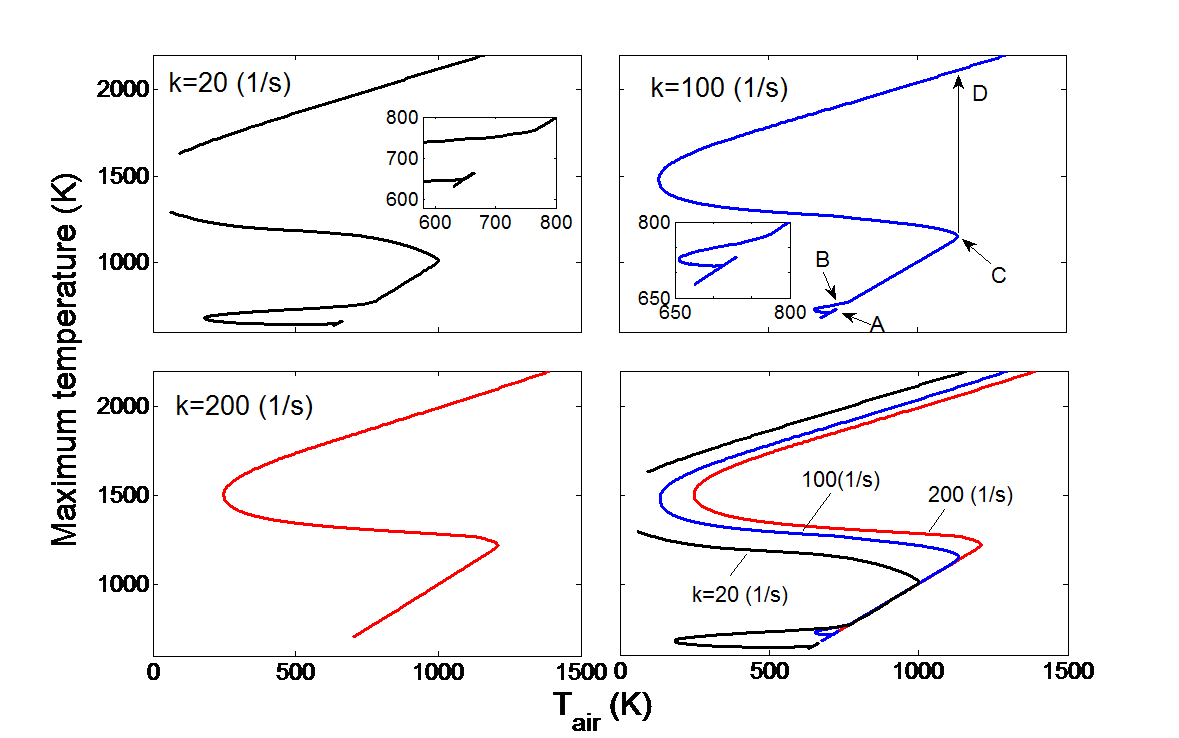
\includegraphics[width=1.0\textwidth]{ch-intro/scurve-zhao.png}
  \normalsize
  \caption{Figure 8 in Law and Zhao~\cite{law12}.  The global response S-curve plotted as maximum temperature versus air-side boundary temperature.  The strain rate varies from 20 to 100 to 200 /s, and the pressure is 1 atm.}
  \label{fig:scurve-zhao}
\end{figure}

Cool flames in nonpremixed systems have been recently studied in counterflow flames~\cite{law12,zhao13,won15,ju16} and microgravity droplet combustion~\cite{nayagam12,farouk15,nayagam15}.  Specifically, Law and Zhao~\cite{law12} and Zhao and Law~\cite{zhao13} computationally investigated nonpremixed counterflow cool flames of $n$-heptane and identified the existence of a secondary S-curve dominated by low-temperature chemistry at low strain rates or high pressures, as shown in Fig.~\ref{fig:scurve-zhao}.  The steady-state response of a one-dimensional reactive system subjected to heat loss can be studied via the S-curve analysis~\cite{lawbook}.  In such an analysis, a system response such as the maximum temperature or radical concentration is monitored for variations of an imposed parameter such as the air temperature, for a given strain rate of the flow, or the system Damk\"ohler number.  For a global one-step overall reaction with large activation energy, the intrinsically nonlinear Arrhenius kinetics frequently yields multiple solutions characterized by an S-shaped response curve, with the lower and upper turning points respectively designate the ignition and extinction states of the system.  Such triple-branch S-curves also frequently emerge for simulations using detailed reaction mechanisms, while more complex response curves with additional turning points have also been obtained, for example for hydrogen oxidation~\cite{kreutz94,fotache98} and methane oxidation~\cite{liu09}.  However, as shown in Fig.~\ref{fig:scurve-zhao}, the secondary S-curve, computationally obtained by Law and Zhao, has its own ignition and extinction turning points and grafts on the lower branch of the primary S-curve. This secondary S-curve predicts the existence of  nonpremixed cool flames at certain conditions.    

Moreover, in microgravity droplet combustion, it was found that the visible flame of large $n$-heptane, $n$-octane, and $n$-decane droplets could transit to a quasi-steady low-temperature-burning mode after extinction of the hot flame due to radiation, suggesting the existence of steady droplet burning sustained by a cool flame~\cite{nayagam15}.   

In Chapter~\ref{ch:NTC} of the dissertation, the computationally predicted nonpremixed counterflow cool flames were experimentally explored.  Ignition and extinction states of nonpremixed cool flames were quantified to provide validation data for further development of low-temperature chemical models.  Computations with detailed chemistry and transport were then conducted to elucidate the thermal and chemical structure of the nonpremixed cool flames, which lays the foundation for understanding the coupling effects of low-temperature chemistry and transport in more complex flows and flame stabilization.

\subsection{Nonpremixed Flame Stabilization and Oscillation}\label{sec:intro-stabilization}

\begin{figure}[t]
  \centering
  \scriptsize
  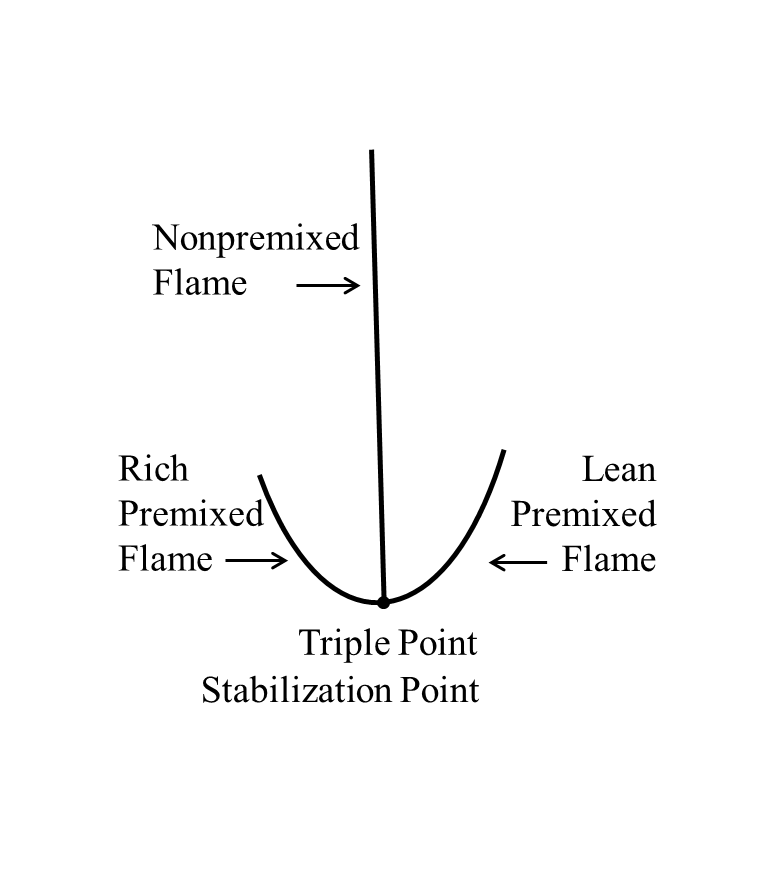
\includegraphics[trim=20mm 24mm 20mm 20mm, clip=true, width=0.5\textwidth]{ch-intro/triple_flame.png}
  \normalsize
  \caption{A schematic plot of the tribrachial flame structure in a coflow mixing layer.}
  \label{fig:triple_flame}
\end{figure}

Nonpremixed jet flames have been extensively studied to understand combustion processes in rocket and diesel engines.  The stabilization and structure of jet flames determine the lift-off height of the flame and are therefore integral to engine design.  Due to the mixing process of the fuel and oxidizer streams in lifted flames at nonautoignitive conditions, the combustion mode is partially premixed, leading to the observation of a two-dimensional tribrachial flame (also known as triple flame)~\cite{buckmaster02}; specifically, a lean and a rich premixed flame wings with a trailing diffusion flame branch, as shown in the schematic plot in Fig.~\ref{fig:triple_flame}.  The point where the three branches intersect is called the triple point and is generally considered to be the stabilization point for nonautoignitive situations. The dynamic balance between the local flame propagation speed and the incoming flow speed is characterized as the stabilization mechanism.  A recent review by Chung~\cite{chung07} discussed the stabilization, propagation, and instability of tribrachial flames, including the effects of concentration gradient~\cite{dold89,hartley91,ghosal00}, velocity gradient~\cite{kim07}, and burned gas expansion~\cite{ruetsch95,lee97,plessing98,kioni99}.  These studies, however, were limited to nonautoignitive conditions, while real engines operate at elevated pressures and temperatures, where autoignition is activated and could interact with the tribrachial flame.

Chung and co-workers~\cite{choi09,choi10,choi12} further conducted a series of experiments to investigate the autoignition characteristics of laminar C$_1$ to C$_4$ fuel jets in a heated air coflow and found that, above certain coflow temperatures, lifted flames could be established through autoignition.  In these studies, both the tribrachial structure for most autoignited cases and a repetitive behavior of extinction and reignition at the critical condition near blowout were observed.  It has been found that the ignition delay time plays an important role for the stabilization of autoignited lifted flames, in such a way that the autoignited liftoff height was correlated with the square of the ignition delay time in some of the investigated cases.

Besides the elevated temperature and pressure effects that initiate autoignition, unsteady flow motion can also modify the flame structure in nonpremixed coflows.  For example, in the experimental investigation of Strawa and Cantwell~\cite{strawa89}, flow instability and flame breakup was achieved by imposing a small-amplitude, periodic velocity fluctuation to nonpremixed jet flames at elevated pressures and low Reynolds numbers.  Later, in the computational study of S\'{a}nchez-Sanz~\emph{et al.}~\cite{sanchezsanz10}, perturbation frequency effects on the thermal and chemical properties of the flame in such periodically time-varying flows were evaluated.  Three regimes were found depending on the flame's Strouhal number, $S = Df/2U$, with $D$ and $f$ denoting the fuel jet diameter and perturbation frequency, respectively.  For small Strouhal numbers ($S = 0.1$), perturbations can travel far downstream, resulting in an oscillating flame.  Flame surface flickering was observed when $S\simeq 0.2$, and vigorous flame pinch-off was observed at $S = 0.5$.  Larger values of $S$ confine the oscillation to the jet's near-exit region with the pulsation having minimal effects on temperature and concentration values.  The unsteadiness in flickering flames also increases pollutant formation, such as soot~\cite{shaddix94} and carbon monoxide~\cite{skaggs96}.  Mohammed~\emph{et al.}~\cite{mohammed98} followed by Dworkin~\emph{et al.}~\cite{dworkin07} conducted computational and experimental studies of $20$ Hz periodically-forced methane/air coflow diffusion flames.  Acetylene production increased~\cite{mohammed98} and the oxidation of CO to CO$_2$ was inhibited~\cite{dworkin07} in the downstream region of the flame at certain times during the flame's cyclic history. 

\subsection{LTC in Flame Stabilization}\label{sec:intro-NTC-stabilization}

As reviewed in previous sections, low-temperature chemistry can induce two-stage ignition and is promoted at elevated pressures.  Consequently, NTC-affected stabilization of nonpremixed lifted jet flames can be potentially important, yet few studies have performed any detailed analysis.  Krisman \emph{et al.}~\cite{krisman15} recently conducted a numerical study of dimethyl ether (DME)/air mixing layer at $40$ atmospheres and air coflow temperatures ranging from $700$ to $1500$ K and observed multibrachial structures in the heat release rate profiles.  The mixture fractions (local composition states) corresponding to the stabilization points defined based on the hydroxyl radical (OH) mass fraction, and the first stage autoignition kernels based on the methoxymethylperoxy radical (CH$_3$OCH$_2$O$_2$), were compared with the most reactive mixture fractions computed from homogeneous autoignition under the same initial conditions.  A transport budget analysis based on selected species was performed to differentiate deflagration from autoignition.

In light of the reported multibrachial structure, showing a modified flame shape from autoignition in the mixing layer, further investigation is warranted to identify the detailed chemical structure and stabilization mechanism of the multibrachial flame.  For example, tools for computational diagnostics, especially for identifying locally dominant chemical reactions, can be employed to understand the controlling chemistry.  Moreover, a direct comparison to homogeneous autoignition is insufficient to understand the transport processes in the current configuration.  In the two-dimensional mixing layer, transport processes in two directions are important: parallel and normal to the mixture fraction gradient, which are due to the transverse stratification of temperature and species and streamwise flow and (flame back) diffusion, respectively.  These considerations would significantly improve the understanding of the role of autoignition upstream of the flame structure and quantitatively identify the controlling kinetics and stabilization mechanism.

In Chapter~\ref{ch:dynamics} of this dissertation, nonpremixed coflow flame dynamics under autoignitive conditions were computationally investigated.  Leveraging the understanding of low-temperature chemistry obtained from nonpremixed counterflow cool flame studies in Chapter~\ref{ch:NTC}, the role of NTC chemistry in flame stabilization at engine relevant conditions will be elucidated.  Moreover, the dominant stabilization mechanism at various flow conditions and the effect of unsteadiness on flame dynamics will be investigated to demonstrate the coupling of fluid dynamics and chemical kinetics to further facilitate future turbulent studies.

\section{Chemistry-Transport Coupling in Soot Emissions}

The second half of this dissertation focuses on the coupling effects of chemical kinetics and transport in sooting flames.  A general question that governs the subsequent investigations is how soot evolution happens in practical engine combustion.  To approach this question, a general overview on soot formation and emission is presented first.  Fuel and flow effects on soot evolution are then reviewed to further motivate this part of work.

\subsection{Soot Mechanisms and Emissions}\label{sec:intro-soot-generic}

In addition to flame dynamics, emissions from combustion processes are also subject to the coupling effects of chemical kinetics and flow dynamics.  One of the dominant pollutants that appears in the form of particulate matter (PM) is carbon black or soot.  Soot particles are undesired products of rich combustion in a wide variety of engineering and natural systems, including transportation and propulsion engines, power generation devices, and fires.  Significant exposure to these black nanoparticles is known to cause heart diseases or lung cancer~\cite{donaldson05}.  In addition, particles emitted from aircraft engines enhance nucleation in the formation of contrails and other atmospheric aerosols~\cite{jensen97,seinfeldbook98}.  Because of the adverse effects on human health and the environment, stringent regulations on emissions from automotive and aircraft engines have been proposed by governments worldwide.

\begin{figure}[t]
  \centering
  \scriptsize
  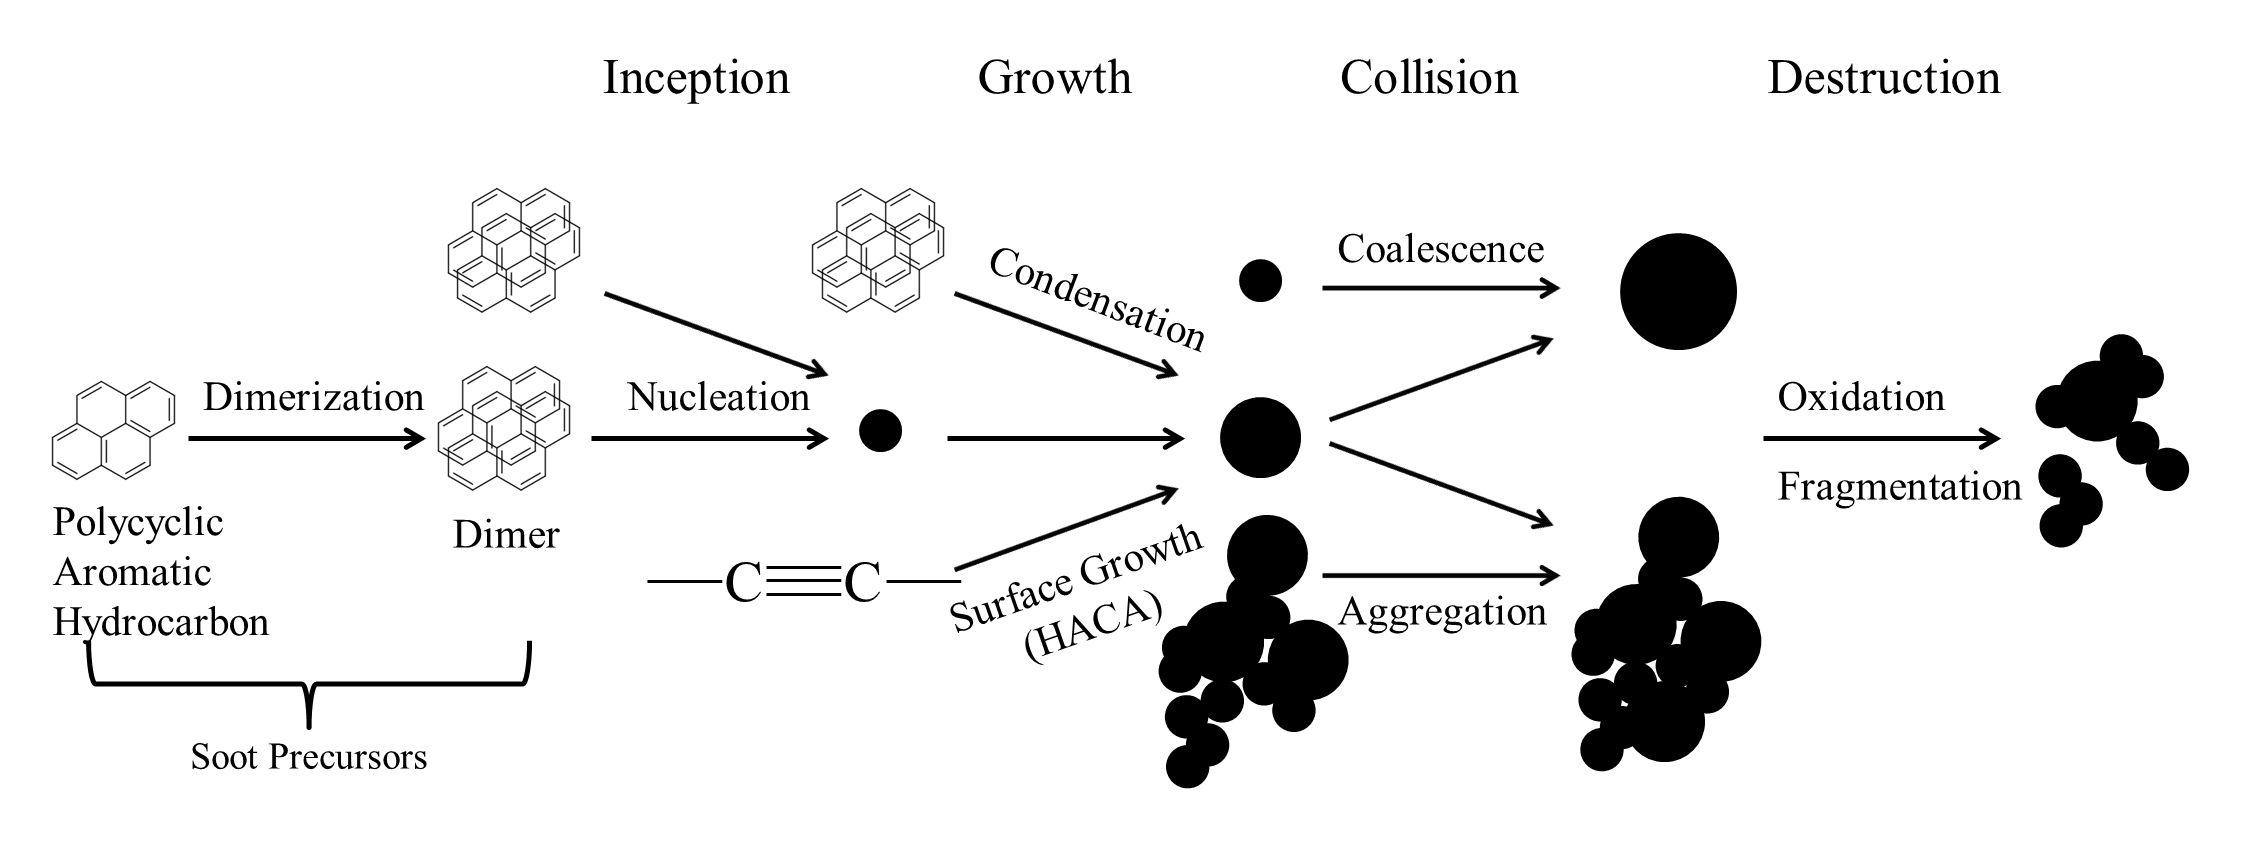
\includegraphics[width=1.0\textwidth]{ch-intro/soot.png}
  \normalsize
  \caption{A schematic drawing of the physical and chemical processes that govern soot evolution.}
  \label{fig:soot}
\end{figure}

The evolution of soot particles is governed by both physical and chemical processes, and the exact mechanisms of soot evolution remain open questions in varying degrees.  A general soot model includes inception, growth, collision, and destruction of soot particles, as shown in the schematic drawing in Fig.~\ref{fig:soot}.  During the inception process, gaseous soot precursors nucleate to form the first soot particle~\cite{schuetz02,wong09,blanquart09c}.  Most soot models consider that these precursors originate in benzene and grow by addition of carbon atoms following the H-abstraction C$_2$H$_2$-addition (HACA) mechanism~\cite{frenklach91}.  Large hydrocarbon molecules are formed from the continuing growth of carbon atoms and appear in ring structures, generally referred as polycyclic aromatic hydrocarbons (PAH)~\cite{schuetz02}.  The subsequent soot growth processes are also closely related to PAH and acetylene, through physical condensation~\cite{park03,mitchell98,mitchell03} and chemical surface growth with the HACA mechanism~\cite{frenklach91}, respectively.  The collision between soot particles also modifies soot morphology.  Two extreme cases are demonstrated in Fig.~\ref{fig:soot}: two small soot particles completely merge to a big spherical particle, or they just barely stick to each other, preserving the total surface area.  Experimentally, soot particles have been found to be both spheres~\cite{zhao05} and fractal aggregates~\cite{jensen07}, as shown in Fig.~\ref{fig:TEM}.  Finally, if the soot particles are exposed to oxidizers such as oxygen and hydroxyl radical, soot fragmentation and oxidation may occur~\cite{kazakov95,neoh81}, resulting in the destruction of soot particles.

\begin{figure}[t]
  \centering
  \scriptsize
  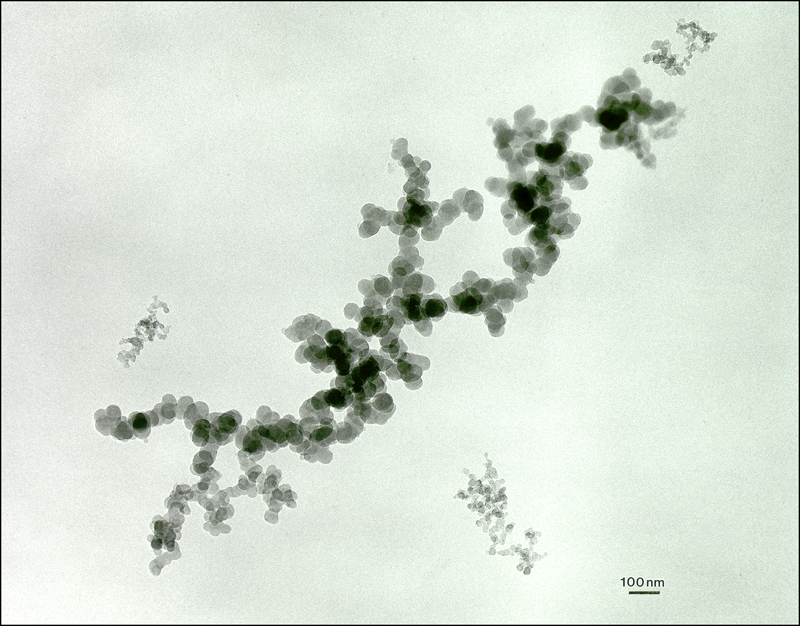
\includegraphics[width=0.6\textwidth]{ch-intro/TEM.jpg}
  \normalsize
  \caption{Transmission electron microscopy (TEM) images of soot aggregate from Jensen \emph{et al.}~\cite{jensen07}.}
  \label{fig:TEM}
\end{figure}

Understanding of soot mechanism has been acquired through experiment and modeling.  While experiments provide data to guide model development and validation, modeling provides insights to help design experiments, improve experimental techniques and understand some of the mechanisms inaccessible in experiments.  However, large uncertainties are still associated with soot models in both the gas phase PAH chemistry and soot dynamics.  Due to limited optical access in sooting flames for online species measurement, validation data for PAH chemical model development is limited.  Therefore, how these large PAH species are formed from smaller species during the fuel breakdown processes needs to be investigated in well-controlled laminar experiments to obtain fundamental understanding of PAH chemical kinetics.  This will then allow the development of relatively high-fidelity soot models to be utilized in, for example, turbulent sooting flame computations to investigate soot evolution in practical engines, for detailed characterization of the flow field and soot would not be available due to experimental limitations.

\subsection{Role of Fuel Structure in PAH Chemistry and Soot Emissions}\label{sec:intro-biofuel}

The utilization of biofuels, which are potential partial replacements for liquid fuels derived from fossil fuels, is garnering wide attention not only because these fuels are renewable, locally producible, and carbon neutral~\cite{liu11} but they also hold potential for positive impacts on particulate matter emission control. Biofuels, including bioalcohols and biodiesels, mainly consist of oxygenated hydrocarbons, such as ethers, alcohols, and esters. When used as additives in conventional diesel fuels, PM emissions have been found to decrease as oxygenated additive concentrations increase~\cite{graboski98}.

However, the precise role of oxygenated additives on the reduction of soot emission has not yet come to a scientific consensus. For example, Frijters and Baert~\cite{frijters06} attributed the PM reduction to the fuel oxygen content, which reduced the local equivalence ratio and, by implication, the flame temperature.  However, even with the same oxygen content, the oxygenates have different efficiencies in the reduction of soot precursor, as Westbrook \emph{et al.}~\cite{westbrook06} found through simulations of premixed $n$-heptane and oxygenates flames.  Furthermore, Pepiot \emph{et al.}~\cite{pepiot08} proposed a structural group contribution approach to interpret diesel engine experimental data and quantify the soot reduction tendency of oxygenated fuels.  As noted by the authors, the aromatics contained in the conventional diesel fuels have very strong sooting tendencies, which are moderated through substitution by the clean-burning oxygenated additives; this replacement effect should be identified and quantified to reveal the role of the oxygen moieties. 

Conversely, a number of studies show that oxygenated fuels do not necessarily have lower sooting tendencies than regular hydrocarbons.  McEnally and Pfefferle~\cite{mcenally05,mcenally11} found that methane coflow nonpremixed flames doped with butanol isomer produce more soot than the undoped ones.  As only $1000$ ppm of each test compound was added to the methane stream, the study was able to identify the direct chemical effects of the addtives.  It was subsequently found that the effect of carbon chain length on soot formation is often larger than the direct chemical effects of oxygen and branches in the carbon chain in promoting soot formation.  Similar conclusions were reached by Camacho \emph{et al.}~\cite{camacho13} by probing the evolution of the detailed particle size distribution function in a set of laminar premixed flames of $n$- and $i$-butane/butanol with fixed C/O ratio and maximum temperature. 

To further explore the sooting characteristics of oxygenated fuels and understand the chemical pathways for soot formation processes, additional well-controlled fundamental experiments and detailed chemical kinetic analyses need to be performed.  In particular, it is recognized that, besides the thermal and replacement effects of oxygenated additives, the residence times of soot precursors are also expected to influence the sooting propensities~\cite{tsuji71,wang14} since soot formation is a kinetically controlled process~\cite{vandsburger85}.

In Chapter~\ref{ch:biofuel} of the dissertation, to investigate the important pathways of soot formation, experimental and computational study first focused on the sooting limits (a residence time effect) of three neat liquid diesel/biofuel components in a stagnation-flow liquid pool system.  With the knowledge on the chemical kinetics of laminar sooting flames, the chemistry-transport coupling effect on soot evolution in turbulent flows was further investigated in Chapter~\ref{ch:bluff}. 

\subsection{Combined Role of Fuel and Turbulence in Soot Emissions}\label{sec:intro-bluff}

Soot formation, growth, and oxidation have been extensively studied in laminar configurations, since flow conditions are better controlled and characterized, which enables detailed analysis of soot evolution~\cite{wang11}.  However, most practical devices operate under turbulent conditions.  The understanding of soot evolution in turbulent reacting flows and the small-scale interactions among soot, turbulence, and chemistry has been aided by Direct Numerical Simulation (DNS).  In the past, these studies have been limited to two-dimensional configurations and/or empirical soot models to limit the computational cost~\cite{yoo07,lignell07,lignell08,bisetti12}, but, recently, Attili~\emph{et al.}~\cite{attili14} performed the first three-dimensional DNS of turbulent nonpremixed jet flames employing a high-order statistical model of soot and a detailed chemical mechanism, which includes the soot precursor naphthalene, and investigated Damk\"{o}hler number effects on soot formation and growth~\cite{attili15}.  Nevertheless, similar to all combustion DNS studies, the Reynolds number was limited to $15,000$, which is lower than most practical combustion systems.

To investigate jet flames at high Reynolds numbers, a combination of experiments~\cite{qamar05,qamar09,lee09,zhang11} and Large Eddy Simulation (LES)~\cite{eiasrag09,mueller12,xuan15} has been used.  However, the jet flame configuration does not contain the more complex fluid dynamics found in practical combustion systems such as recirculating flow.  To bridge this gap, recent experiments and LES have been used to understand the role of recirculating flow on soot evolution in simple, canonical geometries.  Mueller~\emph{et al.}~\cite{mueller13} experimentally and computationally investigated a turbulent nonpremixed bluff body ethylene flame.  Unlike jet flames, surface growth with HACA mechanism was found to dominate in the recirculation zone, highlighting the significance of hydrodynamics on soot evolution.

It is further noted that during the thermal decomposition of hydrocarbon fuels, addition of hydrogen slows down soot formation~\cite{tesner58}.  Extensive laminar studies have been conducted with simplified flow conditions to understand the overall suppression of soot formation in hydrogen-enriched diffusion flames and have attributed such suppression to both dilution and chemistry effects, through the change of the flame temperature and the shift of the balance of the C$_2$H$_2$-addition reactions~\cite{dearden68,du95,gulder96,guo06,zhao14}.  It would be interesting to investigate whether such chemical effects will couple with turbulence in turbulent sooting flames.

In Chapter~\ref{ch:bluff} of the dissertation, a combination of experiments and computations will be utilized to investigate chemical and hydrodynamic effects of fuel composition on the soot evolution in nonpremixed turbulent bluff body flames.  The comparisons between experiments and computations will further validate the LES model and elucidate the important role of chemistry-transport couping in soot evolution in turbulent flow with complex geometry.

\section{Organization of the Dissertation}

This dissertation is aimed to advance the understanding on the coupling effects of chemistry and transport on flame dynamcis and emissions for practical applications.  The first part of the dissertation focuses on flame dynamics at engine relevant conditions.  Specifically, in Chapter~\ref{ch:NTC}, cool flames and low-temperature chemistry in nonpremixed counterflows are investigated both experimentally and computationally.  Leveraging the understanding of low-temperature chemical kinetics in relatively simple flows, in Chapter~\ref{ch:dynamics}, flame dynamics in laminar nonpremixed coflow flames under elevated temperatures and pressures are investigated, and the role of low-temperature chemistry in flame stabilization and oscillation is explored.  The second part of the dissertation focuses on soot emissions with engine relevant fuels in complex flows.  Similar to the structure in flame dynamics studies, in Chapter~\ref{ch:biofuel}, experimental and computational investigations of sooting limits of liquid diesel, bioalcohol, and biodiesel fuels in stagnation-flows are presented.  The same soot model is used to investigate soot evolution in nonpremixed turbulent bluff body flames and compared with experiments, in Chapter~\ref{ch:bluff}.  Finally, in Chapter~\ref{ch:conclusions}, the conclusions of this dissertation are drawn, and suggestions are made for the direction of future work. 

During the preparation of this dissertation, the following work has been compiled for peer-reviewed journal publication.  

\begin{itemize}
  \item \textbf{Chapter~\ref{ch:NTC}:}
    \begin{enumerate}
    \item S. Deng, P. Zhao, D. Zhu, C.K. Law, NTC-affected ignition and low-temperature flames in nonpremixed DME/air counterflow, \textit{Combustion and Flame} \textbf{161} (2014) 1993-1997.
    \item S. Deng, D. Han, C.K. Law, Ignition and extinction of strained nonpremixed cool flames at elevated pressures, \textit{Combustion and Flame} (2016) under review.
    \end{enumerate}
  \item \textbf{Chapter~\ref{ch:dynamics}:}
    \begin{enumerate}[resume]
    \item S. Deng, P. Zhao, M.E. Mueller, C.K. Law, Autoignition-affected stabilization of laminar nonpremixed DME/air coflow flames, \textit{Combustion and Flame} \textbf{162} (2016) 4471-4478.
    \item S. Deng, P. Zhao, M.E. Mueller, C.K. Law, Stabilization of laminar nonpremixed DME/air coflow flames at elevated temperatures and pressures, \textit{Combustion and Flame} \textbf{162} (2016) 4471-4478.
    \item S. Deng, P. Zhao, M.E. Mueller, C.K. Law, Flame dynamics in oscillating flows under autoignitive conditions, \textit{Combustion and Flame} \textbf{168} (2016) 75-82.
    \end{enumerate}
  \item \textbf{Chapter~\ref{ch:biofuel}:}
    \begin{enumerate}[resume]
    \item S. Deng, J.A. Koch, M.E. Mueller, C.K. Law, Sooting limits of nonpremixed $n$-heptane, $n$-butanol, and methyl butanoate flames: Experimental determination and mechanistic analysis, \textit{Fuel} \textbf{136} (2014) 122-129.
    \end{enumerate}
  \item \textbf{Chapter~\ref{ch:bluff}:}
    \begin{enumerate}[resume]
    \item S. Deng, M.E. Mueller, Q.N. Chan, N.H. Qamar, B.B. Dally, Z.T. Alwahabi, G.J. Nathan, Hydrodynamic and chemical effects of hydrogen addition on soot evolution in turbulent nonpremixed bluff body ethylene flames, \textit{Proceedings of the Combustion Institute} \textbf{36} (2017) under review.
    \end{enumerate}
  \item \textbf{Not included in this dissertation:}
    \begin{enumerate}[resume]
    \item P. Zhao, W. Liang, S. Deng, C.K. Law, Initiation and propagation of laminar premixed cool flames, \textit{Fuel} \textbf{166} (2015) 477-487.
    \item D. Han, S. Deng, W. Liang, P. Zhao, F. Wu, Z. Huang, C.K. Law, Laminar flame propagation and nonpremixed stagnation ignition of toluene and xylenes, \textit{Proceedings of the Combustion Institute} \textbf{36} (2017), in press.
    \end{enumerate}
\end{itemize}


%\documentclass[preprint,3p,times,twocolumn]{elsarticleUS}
\documentclass[review,3p,times]{elsarticleUS}
\usepackage{amssymb}
\usepackage{amsmath}
\usepackage{graphicx}
\usepackage{bm}
\usepackage{yhmath}
\usepackage{subfigure}
\usepackage{multirow}
\usepackage{color}
\usepackage{xcolor}
\usepackage{subdepth}
\usepackage[nomarkers,lists]{endfloat}

\def\pp#1#2{\frac{\partial #1}{\partial #2}}

\biboptions{comma,sort&compress}

\journal{Combustion and Flame}

\makeatletter
\def\@author#1{\g@addto@macro\elsauthors{\normalsize%
    \def\baselinestretch{1}%
    \upshape\authorsep#1\unskip\textsuperscript{%
      \ifx\@fnmark\@empty\else\unskip\sep\@fnmark\let\sep=,\fi
      \ifx\@corref\@empty\else\unskip\sep\@corref\let\sep=,\fi
      }%
    \def\authorsep{\unskip,\space}%
    \global\let\@fnmark\@empty
    \global\let\@corref\@empty  %% Added
    \global\let\sep\@empty}%
    \@eadauthor={#1}
}
\makeatother

\begin{document}

\begin{frontmatter}

\title{NTC-affected ignition and low-temperature flames in nonpremixed DME/air counterflow}

\author[Princeton]{Sili~Deng}
\author[Princeton]{Peng~Zhao}
\author[Princeton]{Delin~Zhu}
\author[Princeton,Tsinghua]{Chung K.~Law\corref{cor}}
\cortext[cor]{Corresponding Author: cklaw@princeton.edu}

\address[Princeton]{Department of Mechanical and Aerospace Engineering, Princeton University, Princeton, NJ 08544, USA}
\address[Tsinghua]{Center for Combustion Energy, Tsinghua University, Beijing 100084, China}

\begin{abstract}
An experimental study, supported by computation, was conducted on the coupling of NTC-chemistry and transport in the low-temperature ignition and the associated steady burning in nonpremixed DME/air counterflow.  In particular, the presence of low-temperature chemical reactivity was detected nonintrusively by using a photomultiplier tube combined with a filter to capture the chemiluminescence of HCHO, which is a characteristic intermediate species formed in low-temperature chemistry.  Furthermore, the ignition temperature was determined through high-sensitivity infrared imaging with proper discrimination of the background signal. Experimental results show that the transport-coupled low-temperature, NTC chemical reactivity is enhanced with smaller strain rate, higher air boundary temperature, and is insensitive to the fuel concentration.  These findings agree well with those obtained from computation using detailed chemistry, leading to further identification of the controlling chemistry.
\end{abstract}

\begin{keyword} 
Negative Temperature Coefficient (NTC) \sep Dimethyl Ether (DME) \sep
Nonpremixed Counterflow \sep Low-temperature Chemistry \sep Chemiluminescence
\end{keyword}

\end{frontmatter}

%\clearpage % For word count
\section{Introduction}

Negative temperature coefficient (NTC) refers to the phenomenon that the ignition delay time of a hydrocarbon/air mixture increases with increasing initial temperature within a certain low- to intermediate-temperature range in relation to its adiabatic flame temperature.  This range is typically between $600$ and $800$ K at $1$ atm.  This phenomenon has been extensively studied since it is essential to the combustion of many hydrocarbon fuels, especially for processes associated with engine knock. However, most of these studies and the understanding gained therein are based on homogenous systems, such as those employing shock tubes~\cite{ciezki93}, flow reactors~\cite{wada11}, jet stirred reactors~\cite{veloo13}, and rapid compression machines~\cite{mittal08}.  Since nonuniformities invariably exist in practical combustion systems, the coupling between the NTC chemistry and convective-diffusive transport processes needs to be considered.  It is reasonable to expect that in a chemically reacting flow, when the characteristic transport time becomes comparable to that of the NTC chemical time, the two processes will be strongly coupled to affect the local response.  By the same reasoning, when the characteristic residence time becomes relatively long, the NTC chemistry will be decoupled from the transport processes and the system response will recover to that of the homogeneous mixture.  Indeed, recently Law and Zhao~\cite{law12} and Zhao and Law~\cite{zhao13} have computationally identified the presence of distinctive NTC-affected chemical reactivity and an associated weakly burning flame in the steady counterflow system, showing the existence of a secondary ignition-extinction S-curve grafted onto the lower branch of the primary S-curve. Furthermore this secondary S-curve becomes more pronounced at lower strain rates and higher pressures.

The primary objective of the present investigation is to experimentally explore if the computationally predicted subject phenomenon indeed exists, and to characterize its response if the exploration is affirmative.  The investigation is a challenging one because of the weak reactivity and the correspondingly weak exothermicity involved.

Dimethyl ether (DME) was selected as the fuel for the present study because it is gaseous and is one of the simplest hydrocarbons exhibiting the NTC behavior.  Furthermore, detailed reaction mechanisms for low- and high-temperature DME oxidation~\cite{curran98,fischer00,curran00,zhao08} have been developed and validated for burner stabilized flames~\cite{kaiser00}, nonpremixed counterflow flame ignition~\cite{zheng05}, laminar flame speeds~\cite{qin05}, and studies using rapid compression machines~\cite{mittal08}.  This allows the computational simulation and thereby guidance and verification of the experimentation with moderate confidence. In particular, the present computation was conducted using a skeletal mechanism of $39$ species~\cite{bansal11} reduced from the detailed mechanism of Zhao \emph{et al.}~\cite{zhao08}.

In the following, we shall systematically present the experimental and numerical identification of the NTC-affected ignition and the associated low-temperature flame in the nonpremixed counterflow.  A conference version of the present work was presented in~\cite{deng13}.

\section{Experimental Investigation}

A schematic of the experimental setup is shown in Fig.~\ref{fig:setup}; detailed descriptions of the counterflow experimental apparatus are given in~\cite{fotache95,liu10a}.  Briefly, the apparatus consists of two vertically oriented opposing quartz nozzles with diameters of $20$ mm and separated by $20$ mm.  A heated air or N$_2$ stream is issued from the upper nozzle and impinges against a room-temperature N$_2$-diluted DME steam issued from the lower nozzle.  Both upper and lower streams are shielded by coflowing N$_2$ to minimize disturbance from the environment.  In a typical counterflow ignition experiment, ignition is achieved by gradually increasing the air boundary temperature until a visible flame appears. The exit temperature, measured by a thermocouple with radiation correction~\cite{zheng06}, is then defined as the ignition temperature. Single-point laser Doppler velocimetry (LDV) is used to measure the axial flow velocity along the centerline to determine the local strain rate of the flow.

While the above procedure has been successfully used in previous studies of ignition and the diagnosis of the resulting flame for strongly burning flames, for which the instant of ignition can be observed visually, no bright flame or visually-detectable reaction front could be observed for the present NTC-affected ignition within the temperature range of interests ($600$-$800$ K).  Furthermore, no discernable heat release was detected by using a thermocouple, ostensibly due to the small amount of heat release from the low-temperature chemistry.  In the absence of a flame, it was also not clear the extent of the disturbance introduced by the thermocouple to the flow field as well as the ignition kernel.

In view of the above limitations, we have resorted to optical detection and measurement. A photomultiplier tube (PMT) was subsequently applied to detect any NTC-related chemiluminescence, noting that experimental studies in homogeneous systems have shown that the NTC-induced chemistry have characteristic chemiluminescence spectra, with a small amount of heat release~\cite{sheinson73,ohta91}.  These studies further showed that a large amount of formaldehyde (HCHO) is formed from the low-temperature chemistry and the pale blue chemiluminescence from HCHO characterizes the associated low-temperature reaction~\cite{gaydonbook}.  Based on these characteristics, we designed our experiment as shown in Fig.~\ref{fig:setup}. Here a Hamamatsu 931B PMT combined with focusing lens system and a Newport filter (10BPF10-400) was used to detect the chemiluminescence corresponding to the characteristic wavelength of formaldehyde (peaks around $400$ nm) and to reduce noise light signals from the counterflow chamber. The PMT signal was then collected and processed with a SR510 lock-in amplifier to further diminish the noise.  Results based on this experimentation to demonstrate the existence of the low-temperature chemistry in the counterflow are discussed in Sec.~\ref{sec:4.1}.  This is followed by an investigation based on infrared imaging to identify the state of ignition, in Sec.~\ref{sec:4.2}. 

\begin{figure}[t]
  \centering
  \scriptsize
%  \vspace{-0.1in}
  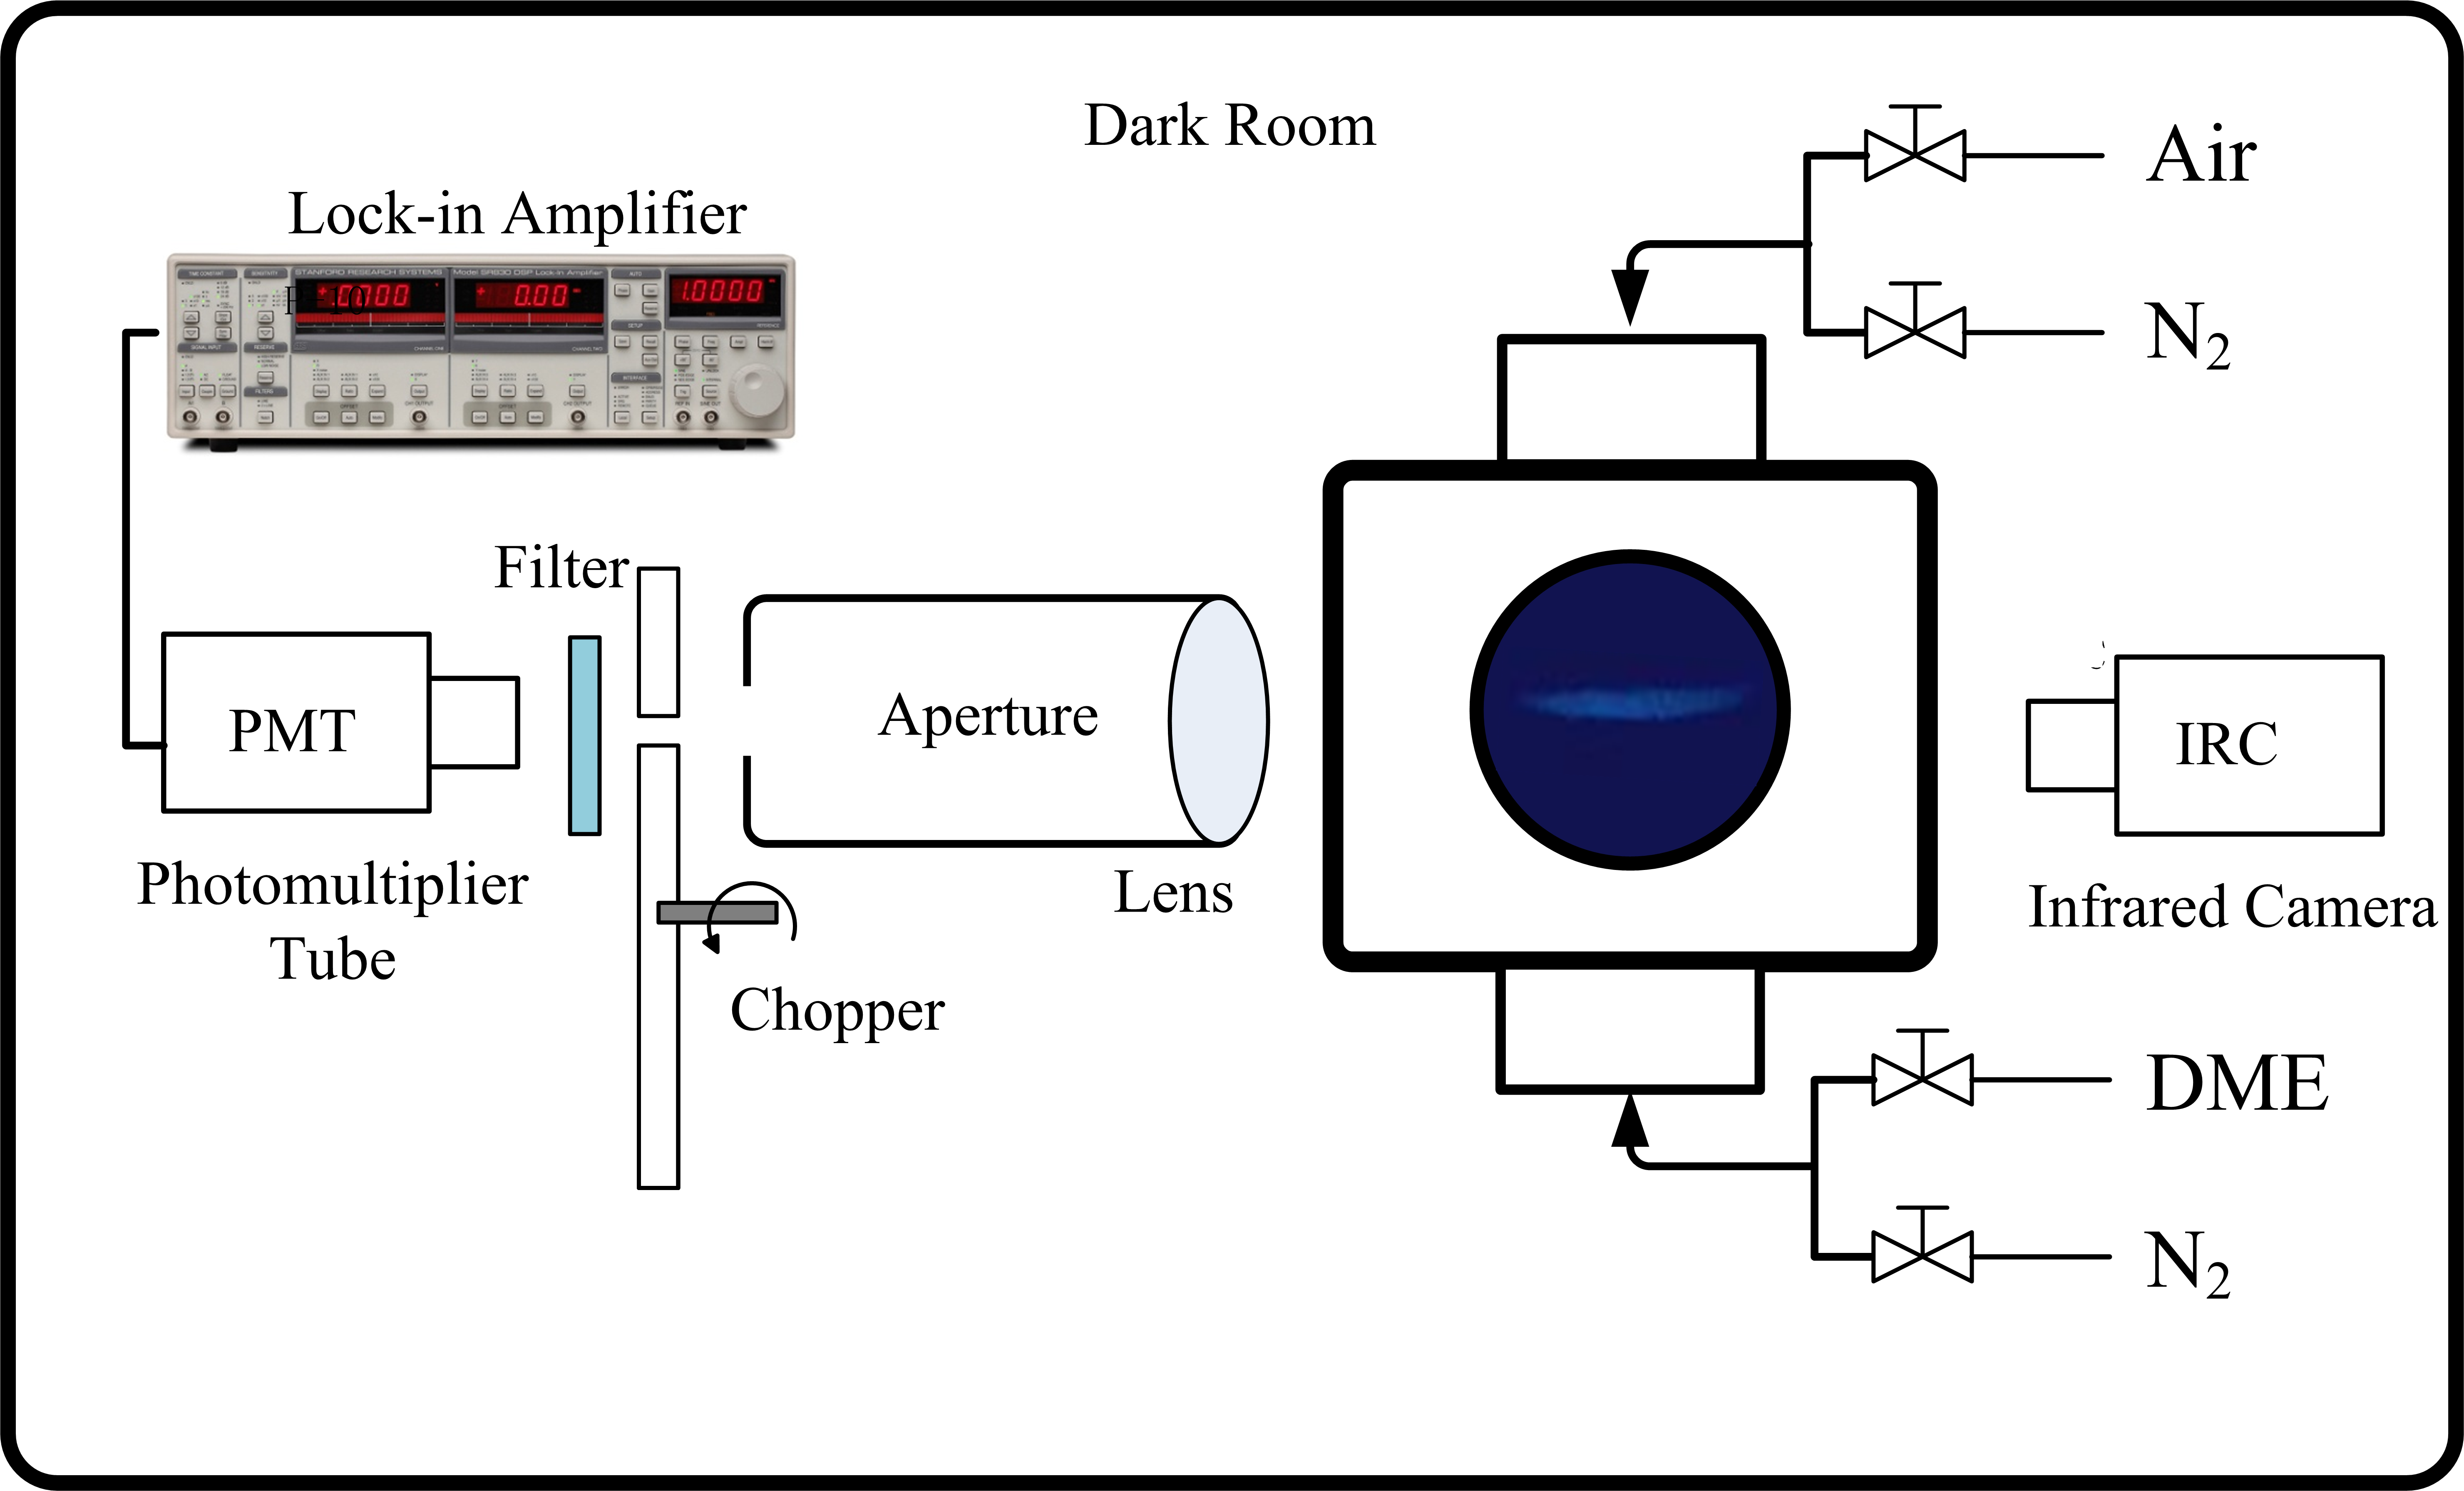
\includegraphics[width=0.8\textwidth]{Experimental_Setup.png}
  \normalsize
%  \vspace{-0.1in}
  \caption{Schematic of the experimental system.}
  \label{fig:setup}
\end{figure}

\section{Computational Investigation}

The steady-state response of a one-dimensional reactive system subjected to heat loss can be studied via the S-curve analysis~\cite{lawbook}. In such an analysis, a system response such as the maximum temperature or radical concentration is monitored for variations of an imposed parameter such as the air temperature, for a given strain rate of the flow, or the system Damk\"ohler number.  For a global one-step overall reaction with large activation energy, the intrinsically nonlinear Arrhenius kinetics frequently yields multiple solutions characterized by an S-shaped response curve, with the lower and upper turning points respectively designate the ignition and extinction states of the system.  Such triple-branch S-curves also frequently emerge for simulations using detailed reaction mechanisms, while more complex response curves with additional turning points have also been obtained, for example for hydrogen oxidation~\cite{kreutz94,fotache98} and methane oxidation~\cite{liu09}. 

The governing equations for the counterflow nonpremixed flame are presented in Giovangigli \emph{et al.}~\cite{giovangigli87}. The numerical code adopted to solve them~\cite{smooke86} employs the damped Newton method and time integration solution scheme, with boundary conditions specified on both sides of the potential flow.  The S-curve marching is performed using the flame-controlling method of Nishioka \emph{et al.}~\cite{nishioka96} with detailed chemistry~\cite{kee89} and transport database~\cite{kee83}.

The critical state of ignition is assessed through the lower turning point of the S-curve.  The simulation conditions are as follows: the fuel-side mixture consists of DME and nitrogen with a fixed temperature of $300$ K, and the oxidizer side is standard air at a high temperature.  The separation distance between the two nozzle exits is $20$ mm, with the origin being fixed at the fuel exit.  To generate an S-curve, marching is performed by either changing the air-side boundary temperature with fixed strain rate or equivalently the strain rate with fixed air-side boundary temperature.  Following Law and Zhao~\cite{law12} and Zhao and Law~\cite{zhao13}, the distinct turning points of the NTC S-curves of DME are captured, and the calculated ignition temperature at different strain rates as well as different boundary fuel concentrations are compared with the experimental results.

\section{Results and Discussion}
\subsection{Identification of the low-temperature, NTC, flame} \label{sec:4.1}

Validation results for the experimental system are shown in Fig.~\ref{fig:M}.  Specifically, when the PMT captures the photons corresponding to the characteristic wavelength of HCHO (peaks around $400$ nm), it outputs negative impulses to the oscilloscope, with the amplitudes of these impulses represent the light intensity.  Figure~\ref{fig:M} shows that such signal intensity drops after replacing either N$_2$-diluted DME with pure N$_2$ issued from the lower nozzle (at point a), or air with N$_2$ issued from the upper nozzle (at point c), hence demonstrating that the signal is due to the simultaneous presence of air and DME.  Since replacing air with the same flow rate of N$_2$ barely affects the temperature profile and the flow field, the signal difference between the air/DME and N$_2$/DME cases indicates the existence of NTC chemical activities.  It is noted that the signal from N$_2$/DME thermal pyrolysis is minimal in the present study, such that the difference in the chemically reactive and non-reactive cases can be completely attributed to the low-temperature oxidation chemistry.  


\begin{figure}[t]
  \centering
  \scriptsize
  \vspace{-0.1in}
  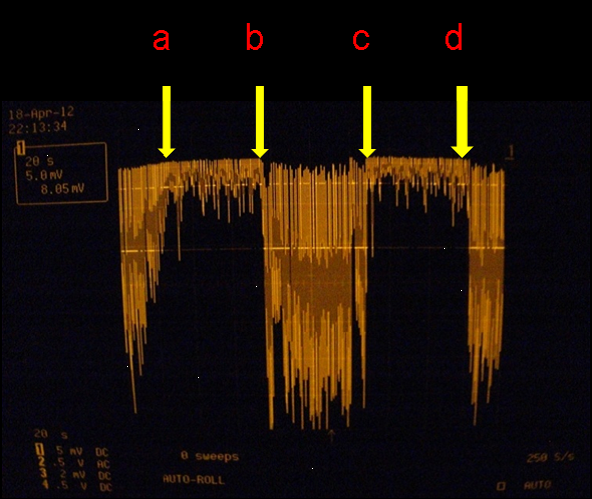
\includegraphics[width=0.5\textwidth]{M.png}
  \normalsize
%  \vspace{-0.1in}
  \caption{"M" shaped signal. a.~Switch Air/DME to Air/N$_2$; b.~Switch Air/N$_2$ to Air/DME; c.~Switch Air/DME to N$_2$/DME; d.~Switch N$_2$/DME to Air/DME.}
  \label{fig:M}
\end{figure}

In Fig.~\ref{fig:PMT}, the chemiluminescence intensity from the HCHO under the strain rates of $40$, $60$, and $100$ /s were measured as a function of the air boundary temperature.  The time-averaged signal were acquired by the lock-in amplifier with an integration time of three seconds to minimize the noise, and the error bars show the standard deviation of the signals based on $1000$ samplings. The results clearly show that the low-temperature chemistry becomes more pronounced at higher air temperatures and lower strain rates, with more HCHO produced and therefore stronger chemiluminescence from it.

\begin{figure}[t]
  \centering
  \scriptsize
  \vspace{-0.1in}
  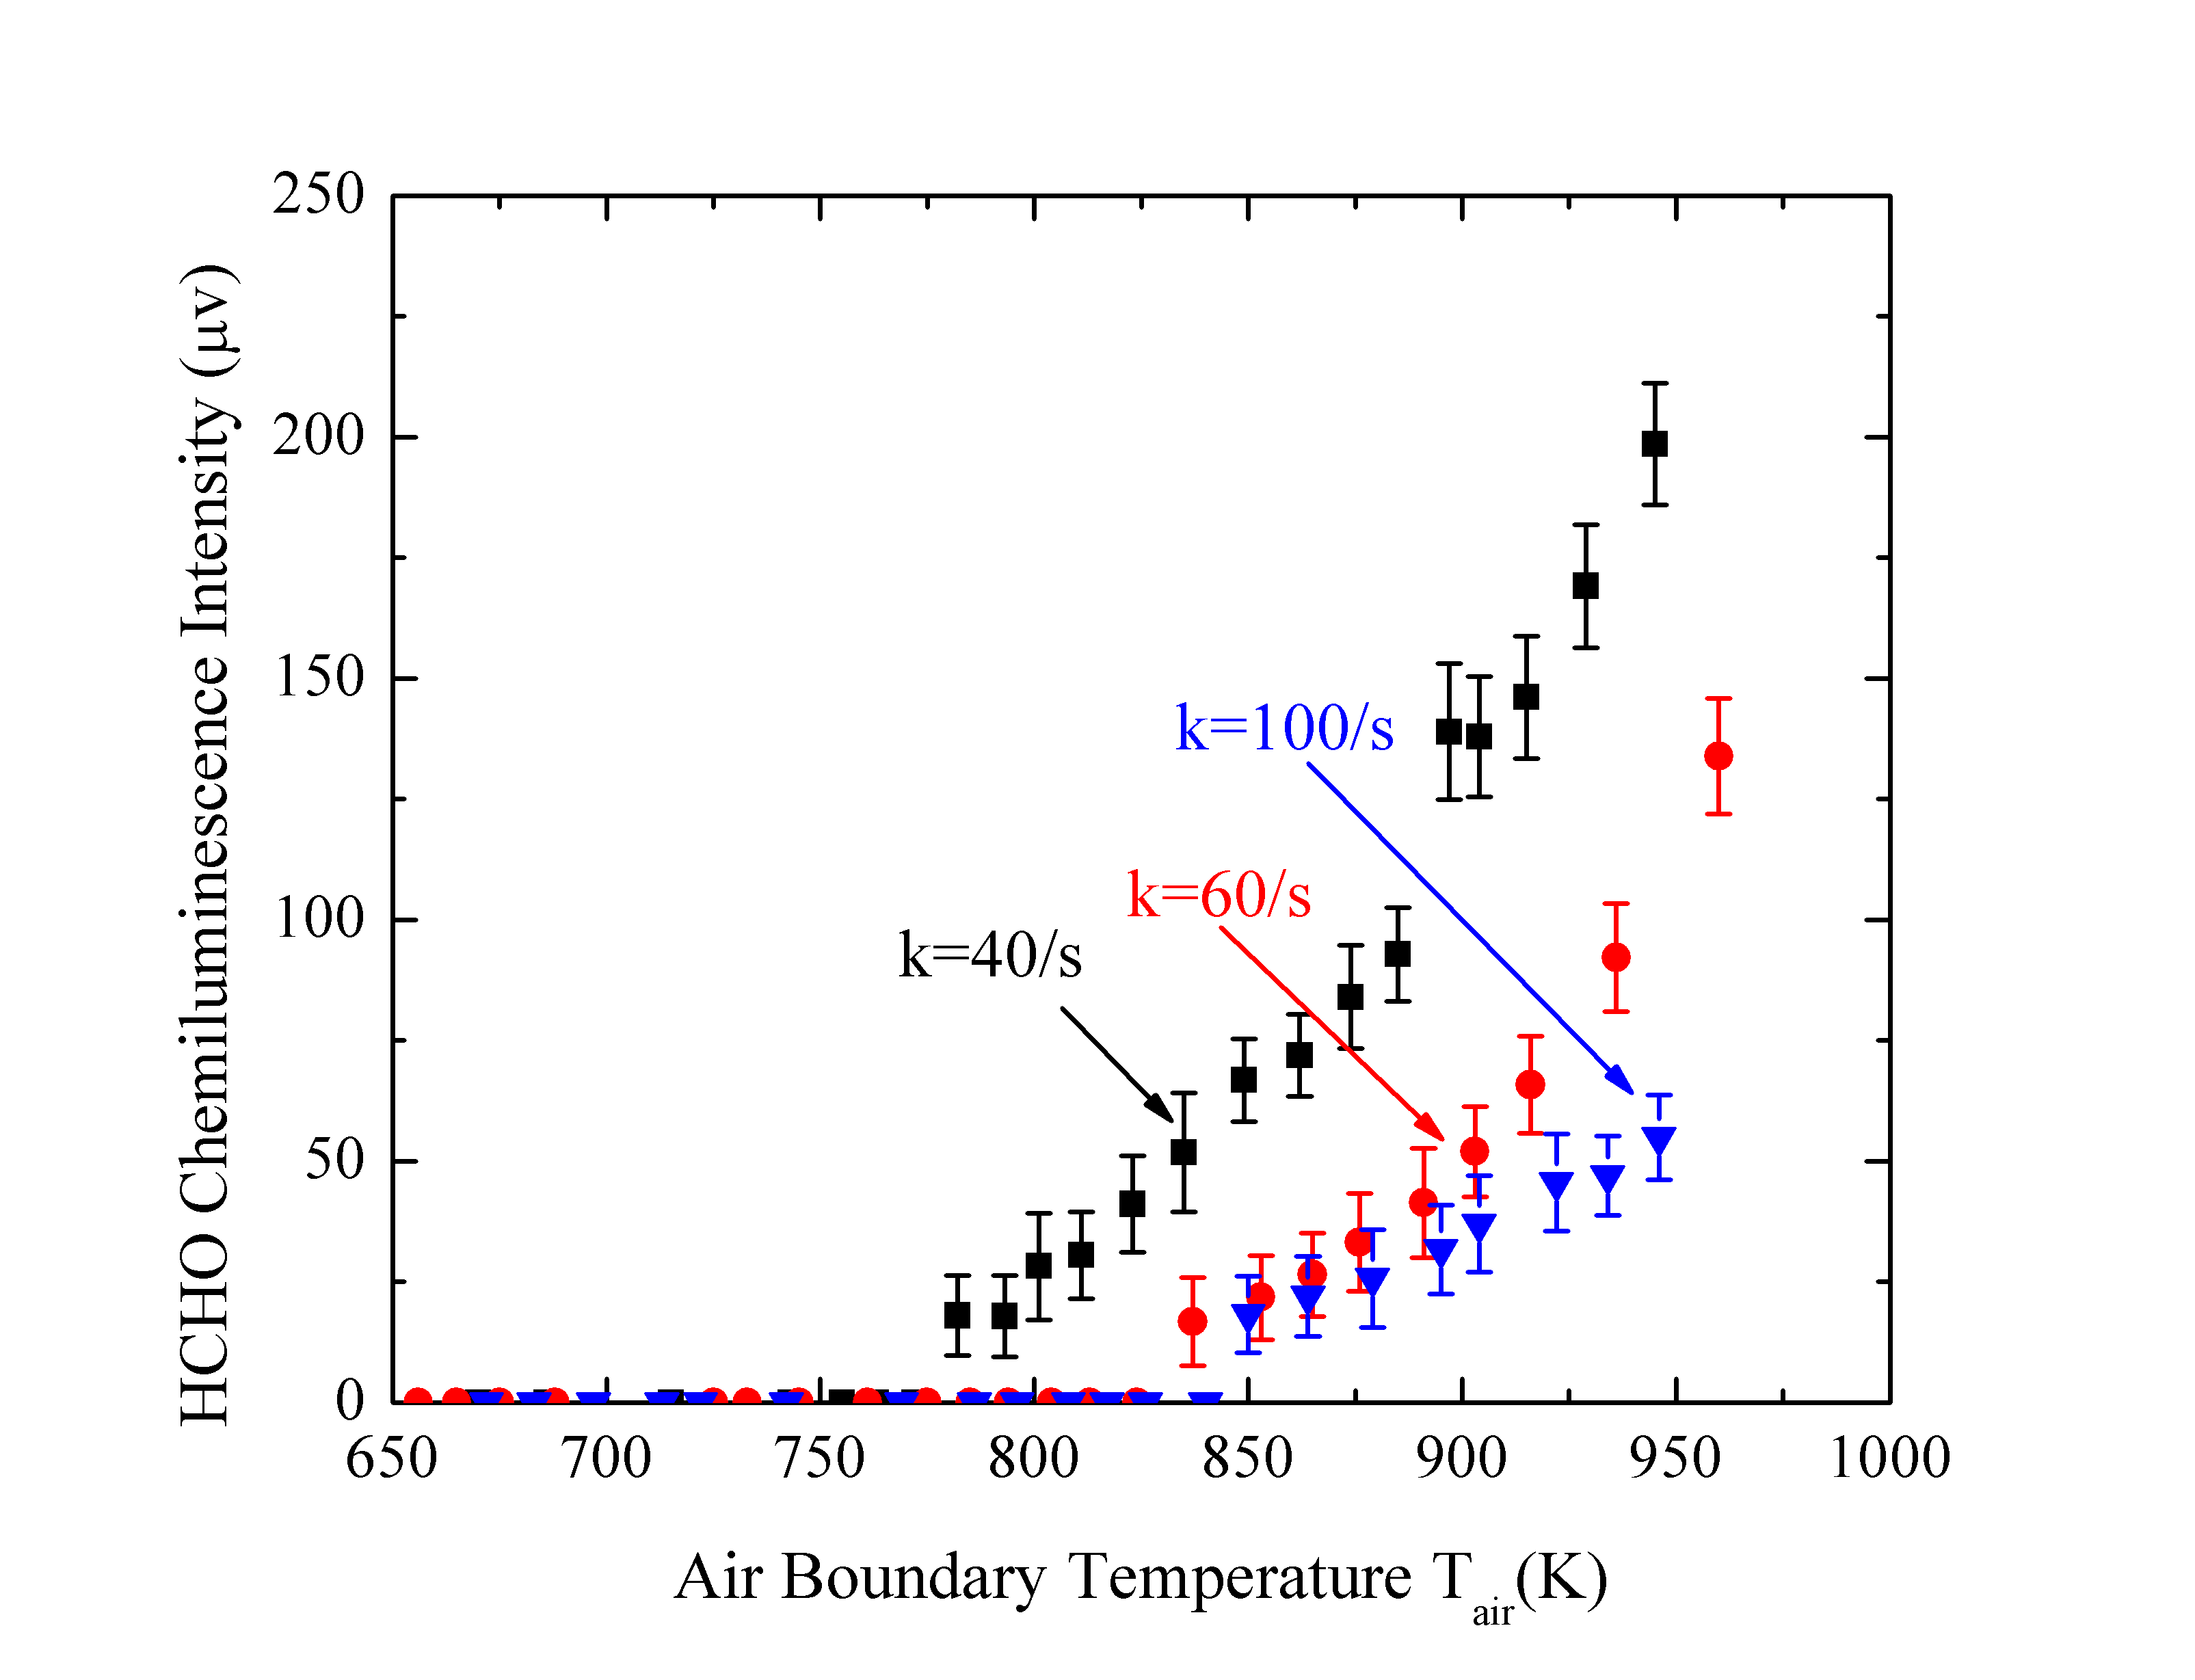
\includegraphics[width=0.6\textwidth]{PMT.png}
  \normalsize
  \vspace{-0.1in}
  \caption{HCHO chemiluminescence intensity at different air boundary temperatures under various strain rates.}
  \label{fig:PMT}
\end{figure}

The above experimental observations are further corroborated by the calculated results of the maximum formaldehyde (HCHO) mole fraction versus the air temperature for $30\%$ DME in nitrogen, for different strain rates.  Figure~\ref{fig:Scurve-SR} shows the calculated secondary S-curve characterized by the low-temperature chemistry.  It is seen that the upper branch solution, designating the state of the low-temperature flame, shows the same experimental trend of increasing HCHO concentration with increasing air temperature and decreasing strain rate.  We have therefore identified the presence of NTC-related chemical reactivity in the strongly transport-affected, nonpremixed counterflow.  The fact that this chemical reactivity is localized in a thin “flame” region is demonstrated in the next section.

\begin{figure}[t]
  \centering
  \scriptsize
  \vspace{-0.1in}
  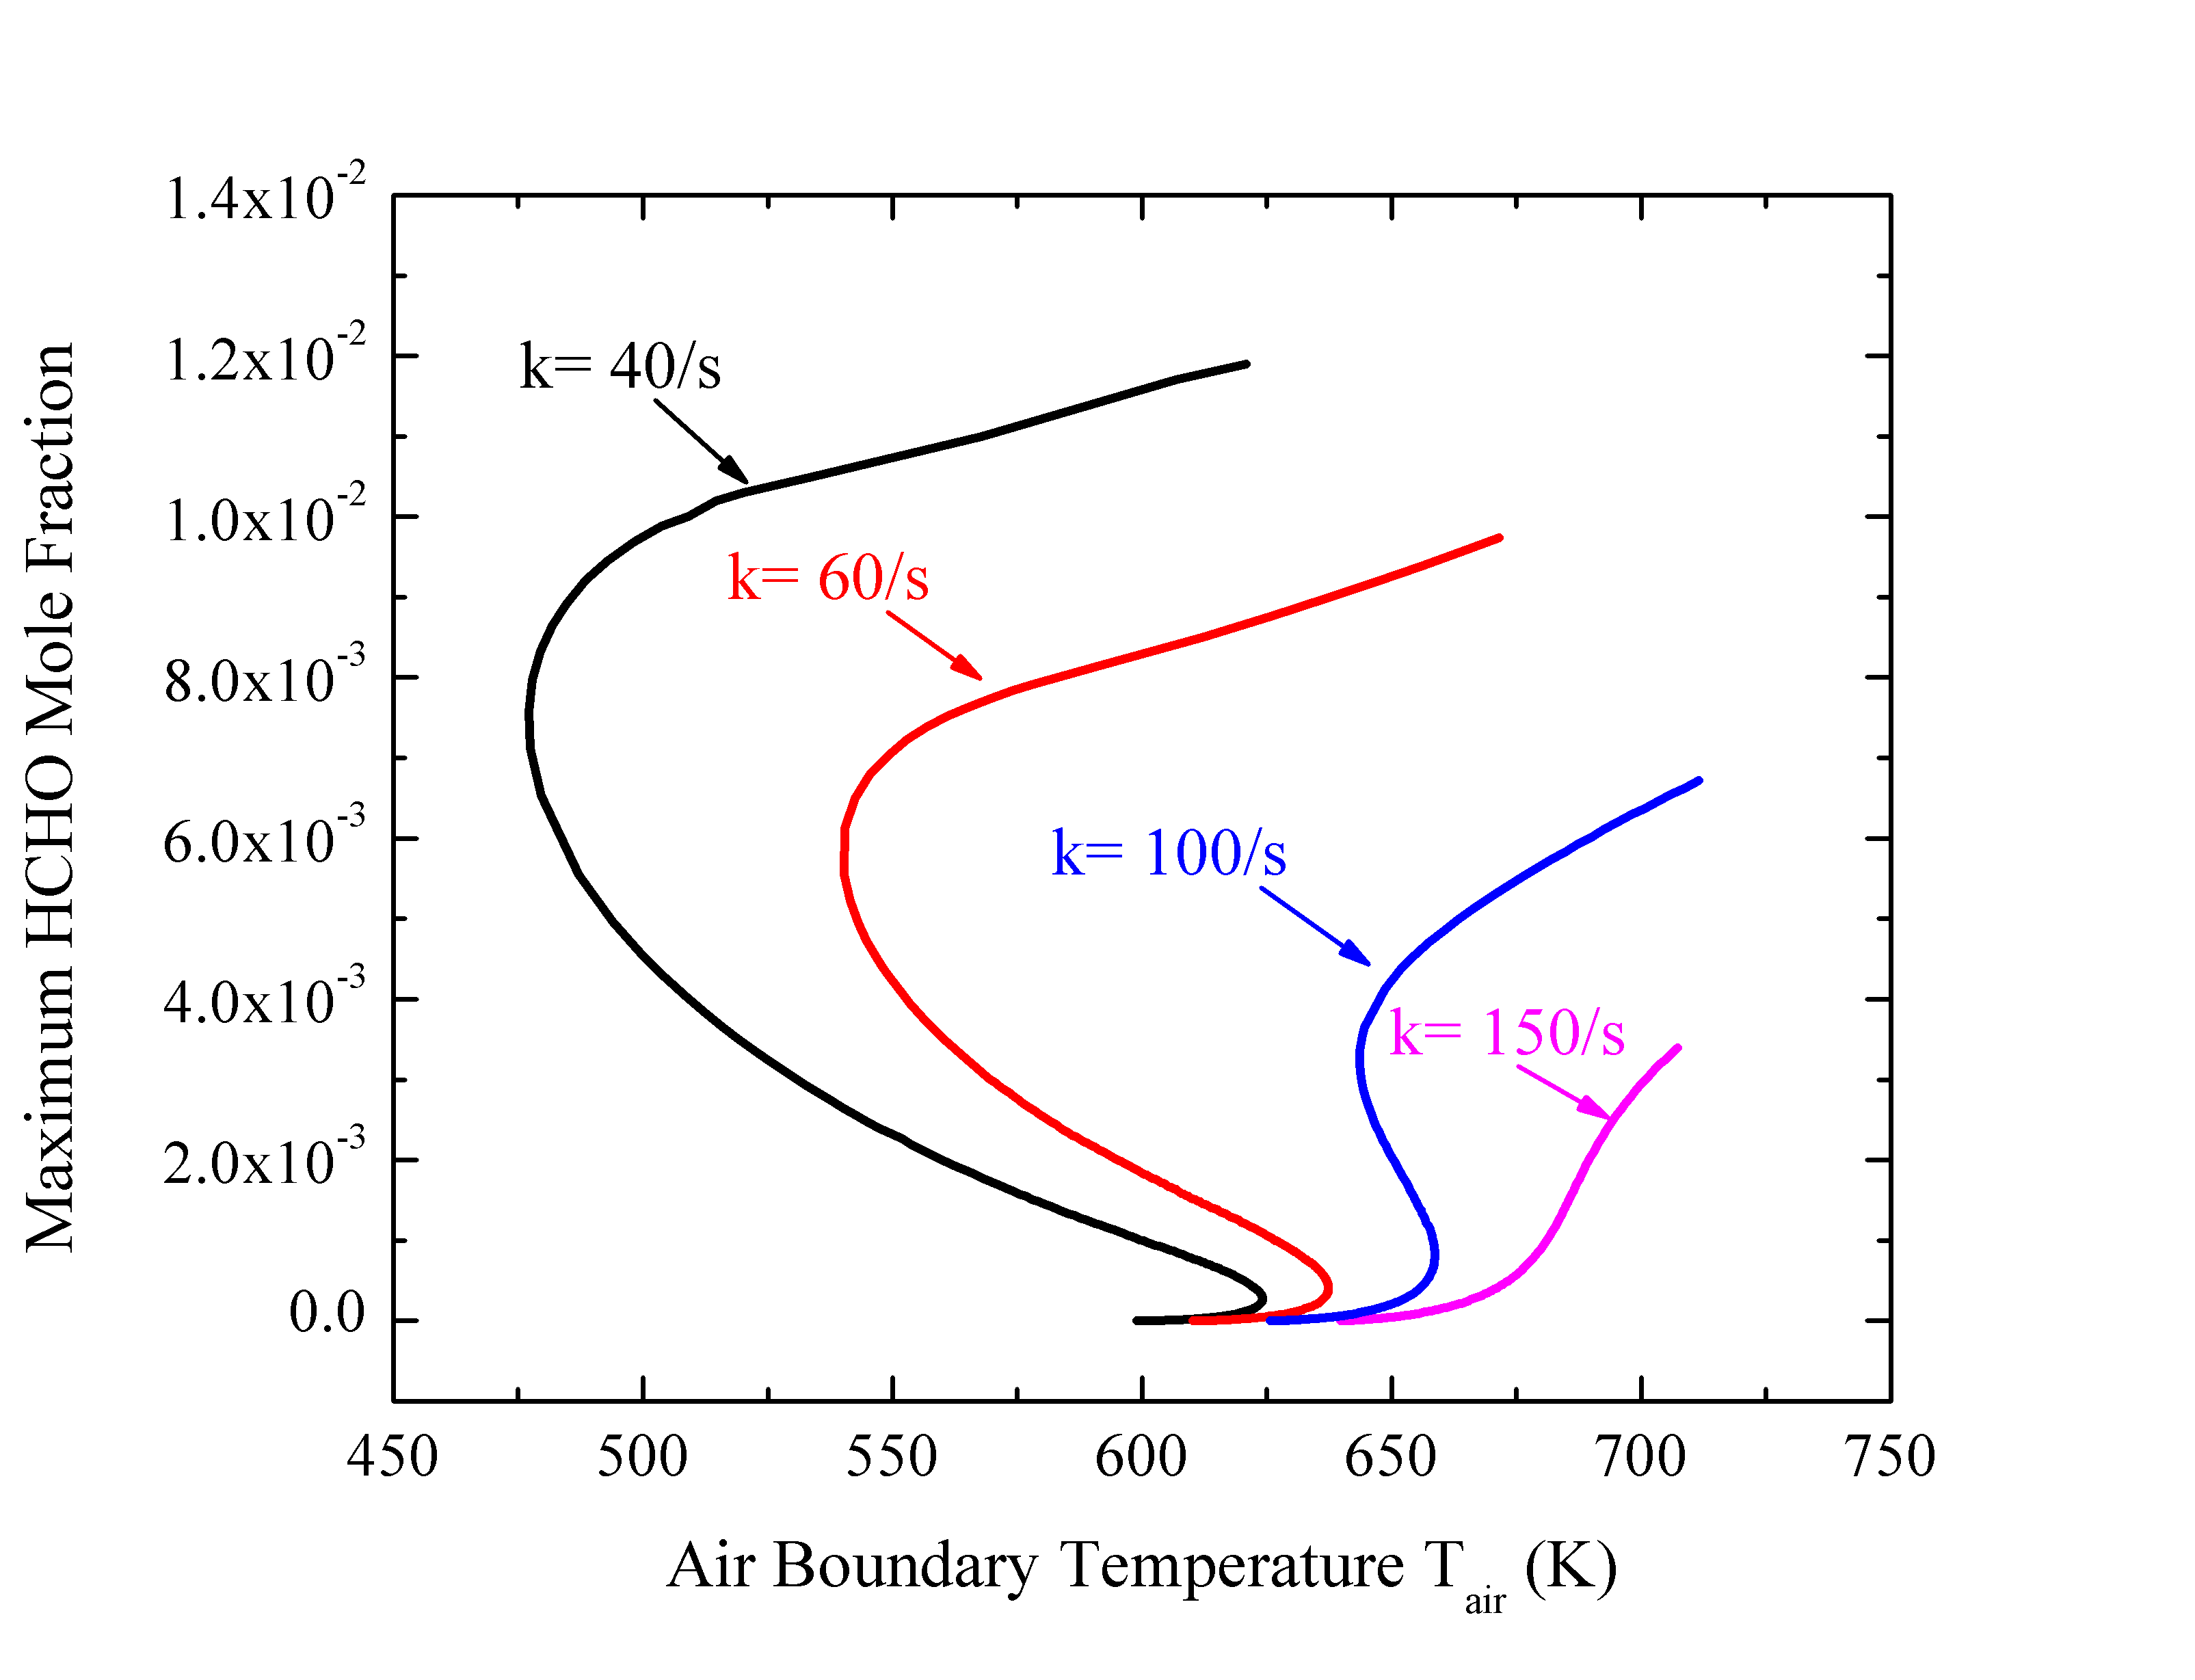
\includegraphics[width=0.6\textwidth]{Scurve-SR.png}
  \normalsize
  \vspace{-0.1in}
  \caption{Maximum HCHO mole fraction of $30\%$ DME at different air boundary temperatures under various strain rates.}
  \label{fig:Scurve-SR}
\end{figure}

\subsection{Determination of ignition temperature} \label{sec:4.2}

\begin{figure}[ht]
  \centering
  \scriptsize
  \vspace{0.1in}
  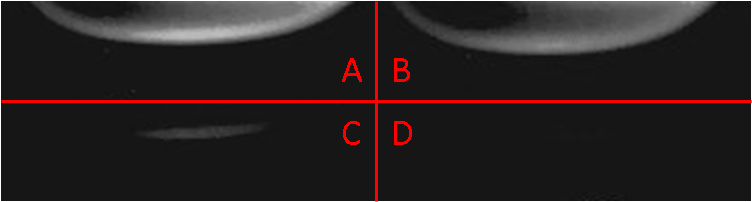
\includegraphics[width=0.5\textwidth]{IR.png}
  \normalsize
%  \vspace{-0.1in}
  \caption{A/B: Heated air/N$_2$ against DME counterflow IR images at ignition (atmospheric pressure, strain rate $60$ /s); C/D: Difference between A/B and B.}
  \label{fig:IR}
\end{figure}

We now proceed to detect the state of ignition of the NTC-flame, as identified by the lower turning points in Fig.~\ref{fig:Scurve-SR}.  Since the chemiluminescence intensity from the above experimentation is not strong enough to detect the low level of HCHO concentration at ignition, we have resorted to capturing the infrared radiation from the ignition process by using a highly sensitive infrared camera, FLIR SC640 (with the thermal sensitivity about $60$ mK at $303$ K), as shown on the right part of Fig.~\ref{fig:setup}.  The brightness of the IR images in Fig.~\ref{fig:IR} indicates the IR radiation intensity, with the bright color denoting higher radiation intensity than the dark color.  Since both the air/DME and N$_2$/DME flows now radiate infrared signals when heated due to the excitation of the vibrational modes of the gas molecules in the thermal mixing layer, the “background” N$_2$/DME signal needs to be subtracted out from the air/DME signal so as to isolate/identify the emission due to the low-temperature chemical reactivity.  Consequently, by gradually increasing the air boundary temperature, and by setting the IR radiation intensity of the N$_2$/DME flow as the reference state, the first appearance of an excess signal from the air/DME flow would indicate the onset of ignition.  In practice, when the air boundary temperature reaches the regime of interests, only $1$ K is increased each time at the air boundary before the flow becomes steady again.  It is fairly clear that at a certain temperature, which is defined as the ignition point, the signal from air/DME starts to exceed that of the reference state.  Such temperature measurements are repeatable within $\pm 2$ K.  A typical result is shown in Fig.~\ref{fig:IR}, in which the A and B panels are the raw IR signals for heated air and N$_2$ against DME, which are respectively reactive and nonreactive.  Panels C and D respectively show the residue signals of panels A and B after the background signal from panel B is subtracted; the null signal for D is obtained by default.  The temperature at which a discernable image of radiation is detected is then identified as that of ignition, as is the case for panels A/C, for the corresponding strain rate.

The localized nature of the IR radiation, shown in panel C, then also supports the notion that the chemical reactivity observed herein has the characteristic of a flame, in support of the interpretation of the chemiluminescence signal reported in the previous section.

Figure~\ref{fig:Ign-SR} shows the IR measurements of the low-temperature chemistry induced ignition, as determined through the above procedure, as a function of the strain rate.  The uncertainty bars account for those from the thermocouple radiation correction as well as reproducibility of the experimental measurements.  Due to the moderate flow field temperatures and the high sensitivity of the thermocouple, the uncertainty bars of the ignition temperatures are quite small.  These experimental values are then compared with those corresponding to the calculated lower, ignition turning points.  Figure~\ref{fig:Ign-SR} shows satisfactory agreement, with the average temperature difference being within $20$ K.

Sensitivity analysis was further performed for the state of ignition, as shown in Fig.~\ref{fig:Sen_SR}.  It is seen that the controlling chemistry is indeed the low tempearature chemistry, corresponding to the first stage ignition of the homogeneous autoignition process in the NTC-affect regime.  More specifically, the first two most important reactions that promote the low temperature chemistry induced ignition are the oxygen combination reaction: CH$_2$OCH$_2$O$_2$H+O$_2$ $\Leftrightarrow$ O$_2$CH$_2$OCH$_2$O$_2$H and the isomerization reaction: CH$_3$OCH$_2$O$_2$ $\Leftrightarrow$ CH$_2$OCH$_2$O$_2$H, while the most important retarding reaction is the $\beta$-scission reaction: CH$_2$OCH$_2$O$_2$H $\Leftrightarrow$ OH+$2$HCHO.  These two groups of reactions compete for the CH$_2$OCH$_2$O$_2$H radicals and as such function oppositely.

\begin{figure}[t]
  \centering
  \scriptsize
  \vspace{-0.1in}
  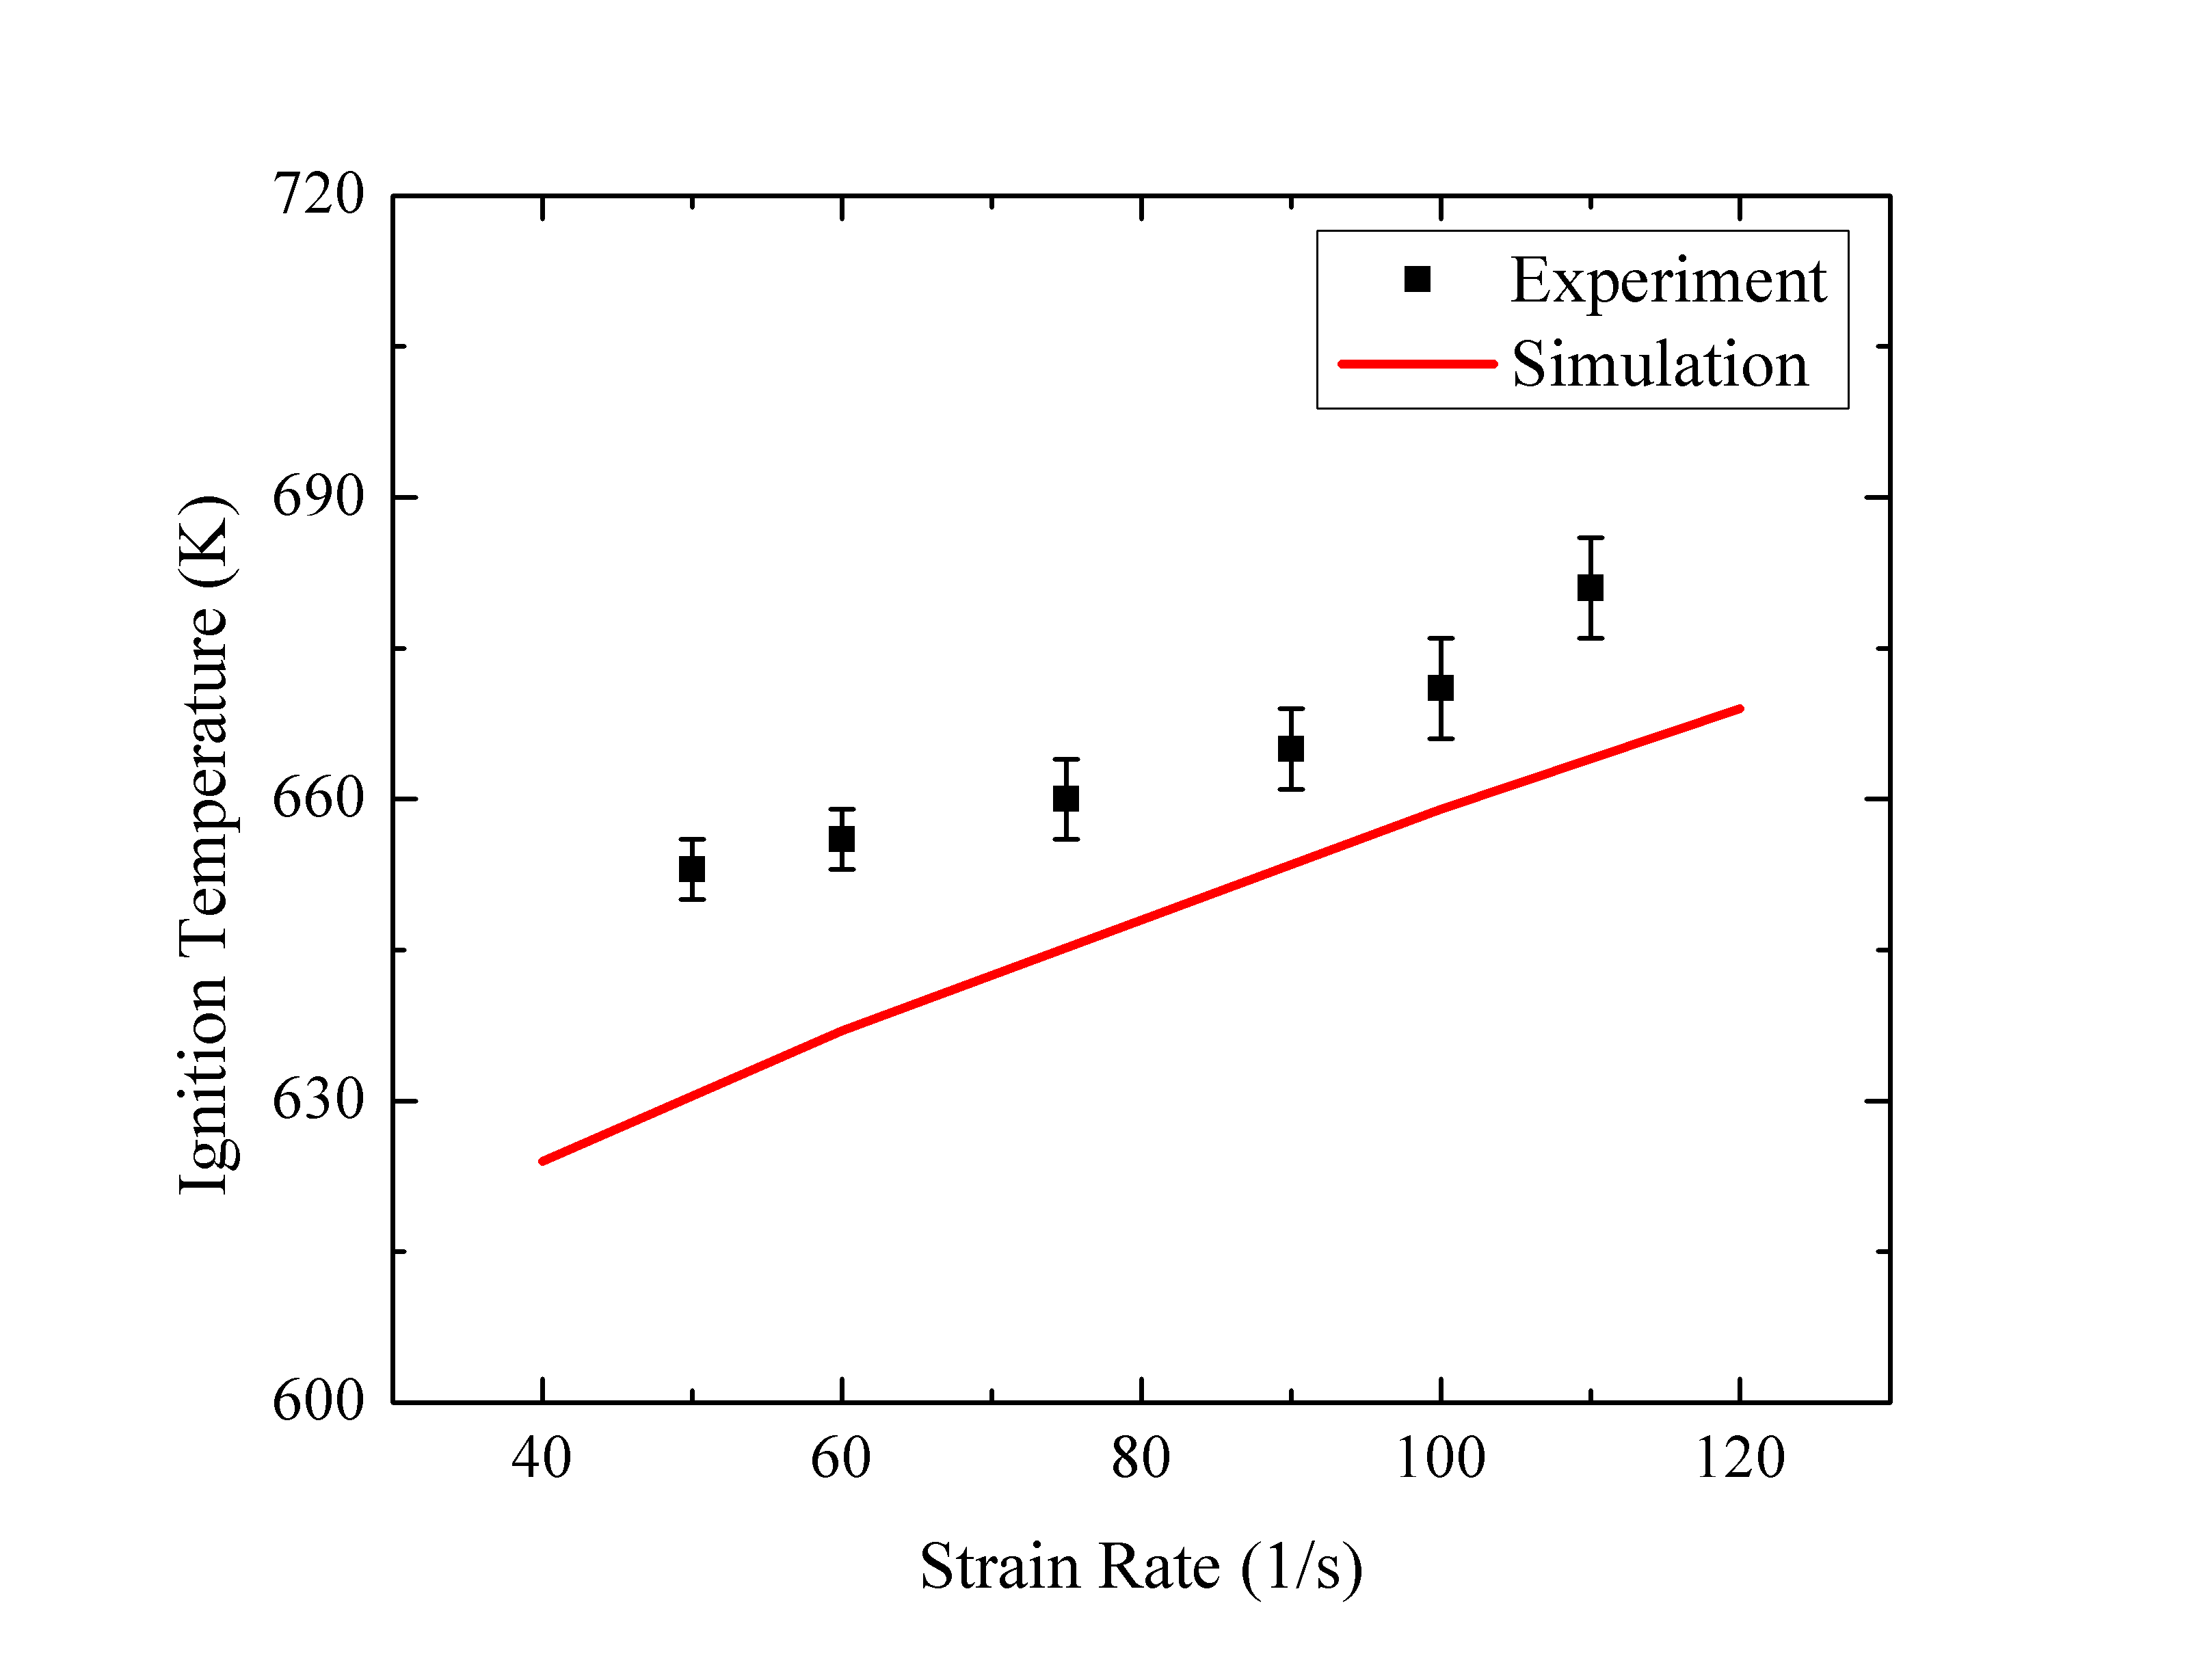
\includegraphics[width=0.6\textwidth]{Ign-SR.png}
  \normalsize
  \vspace{-0.1in}
  \caption{Calculated and observed ignition temperatures of $30\%$ DME under various strain rates.}
  \label{fig:Ign-SR}
\end{figure} 

\begin{figure}[t]
  \centering
  \scriptsize
  \vspace{-0.1in}
  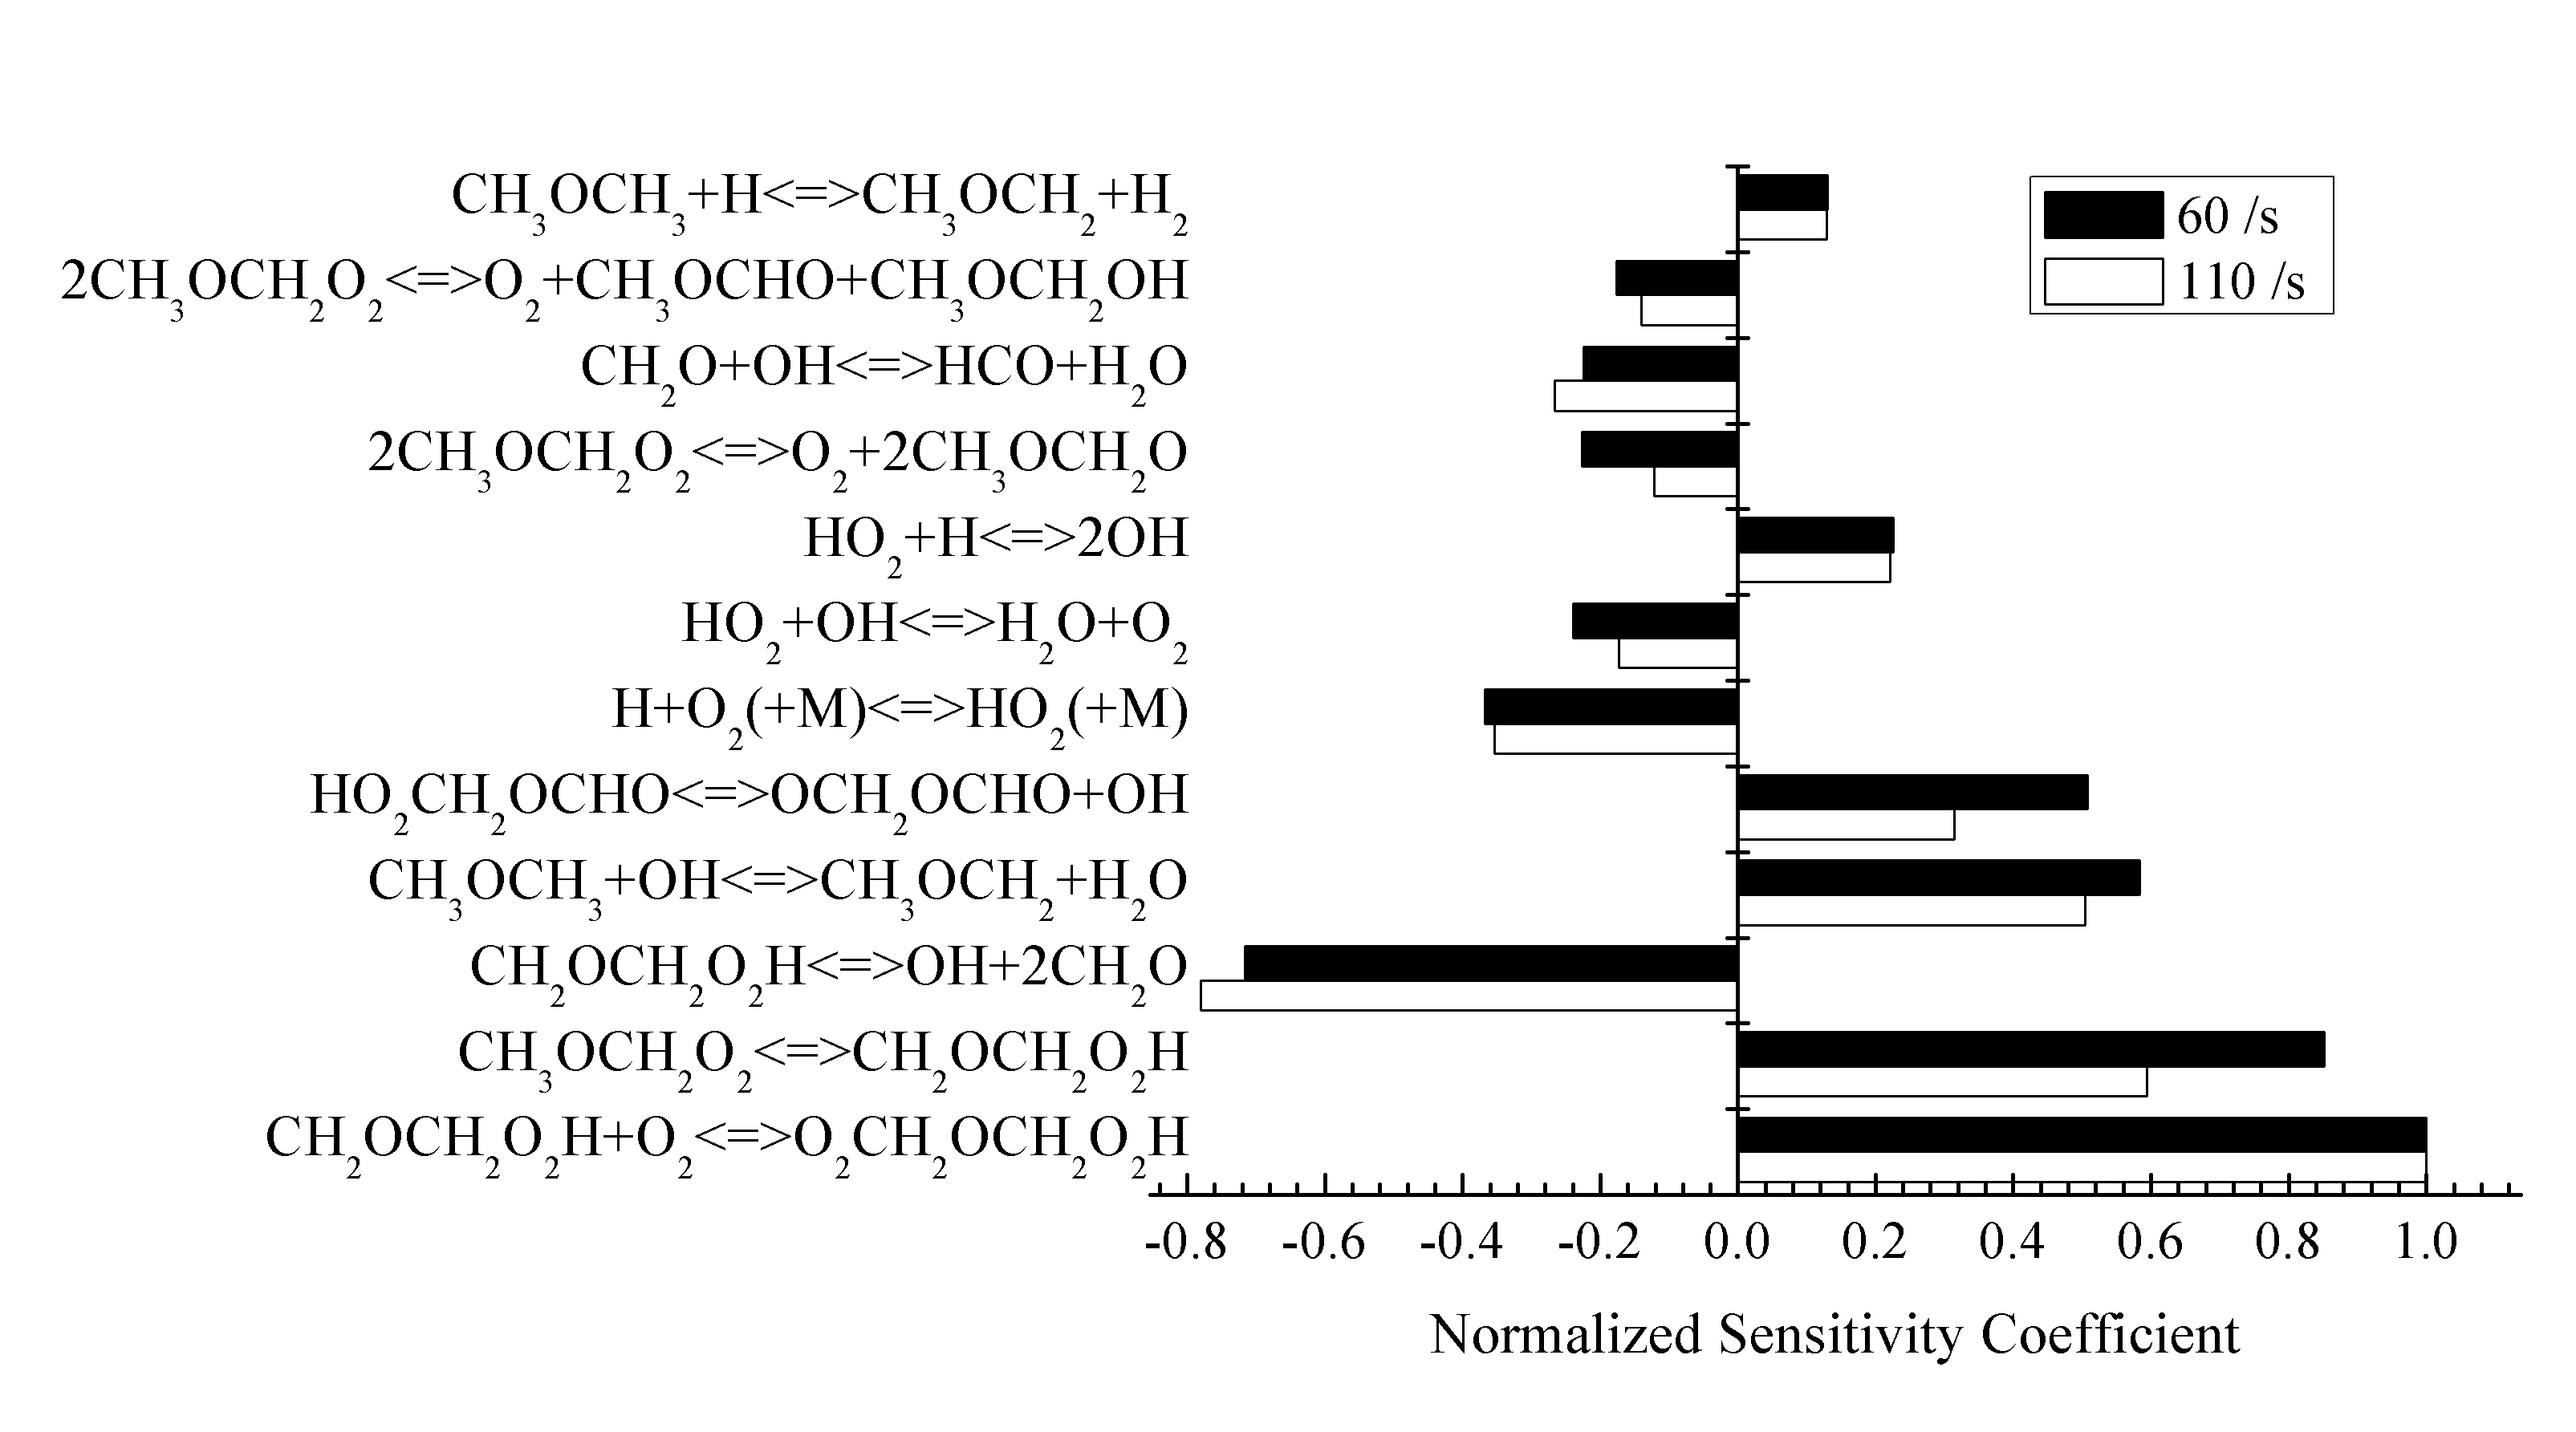
\includegraphics[width=0.7\textwidth]{Sen_SR.png}
  \normalsize
  \vspace{-0.1in}
  \caption{Sensitivity analysis on low and high strain rate cases: DME mole fraction is $30\%$.}
  \label{fig:Sen_SR}
\end{figure}

In addition to the effects of strain rate on the ignition temperature, we have also evaluated the effects of DME concentration, shown and compared with the simulation results in Fig.~\ref{fig:Ign-Con}.  The simulation result basically demonstrates the insensitive nature of the NTC-affected ignition temperature to the variation of the boundary DME concentrations over an extensive range of DME concentrations, under a fixed strain rate of $60$ /s.  The experimental results again show good agreement with the simulation results.  This effect corresponds to the insensitive nature of the equivalence ratio in the low-temperature chemistry, given the fact that the first-stage delay is insensitive to the equivalence ratio in the homogeneous autoignition process~\cite{zhao13}.  Sensitivity analysis corresponding to different boundary DME concentrations were also carried out, showing the same controlling chemistry as that of Fig.~\ref{fig:Sen_SR}.

\begin{figure}[t]
  \centering
  \scriptsize
  \vspace{-0.1in}
  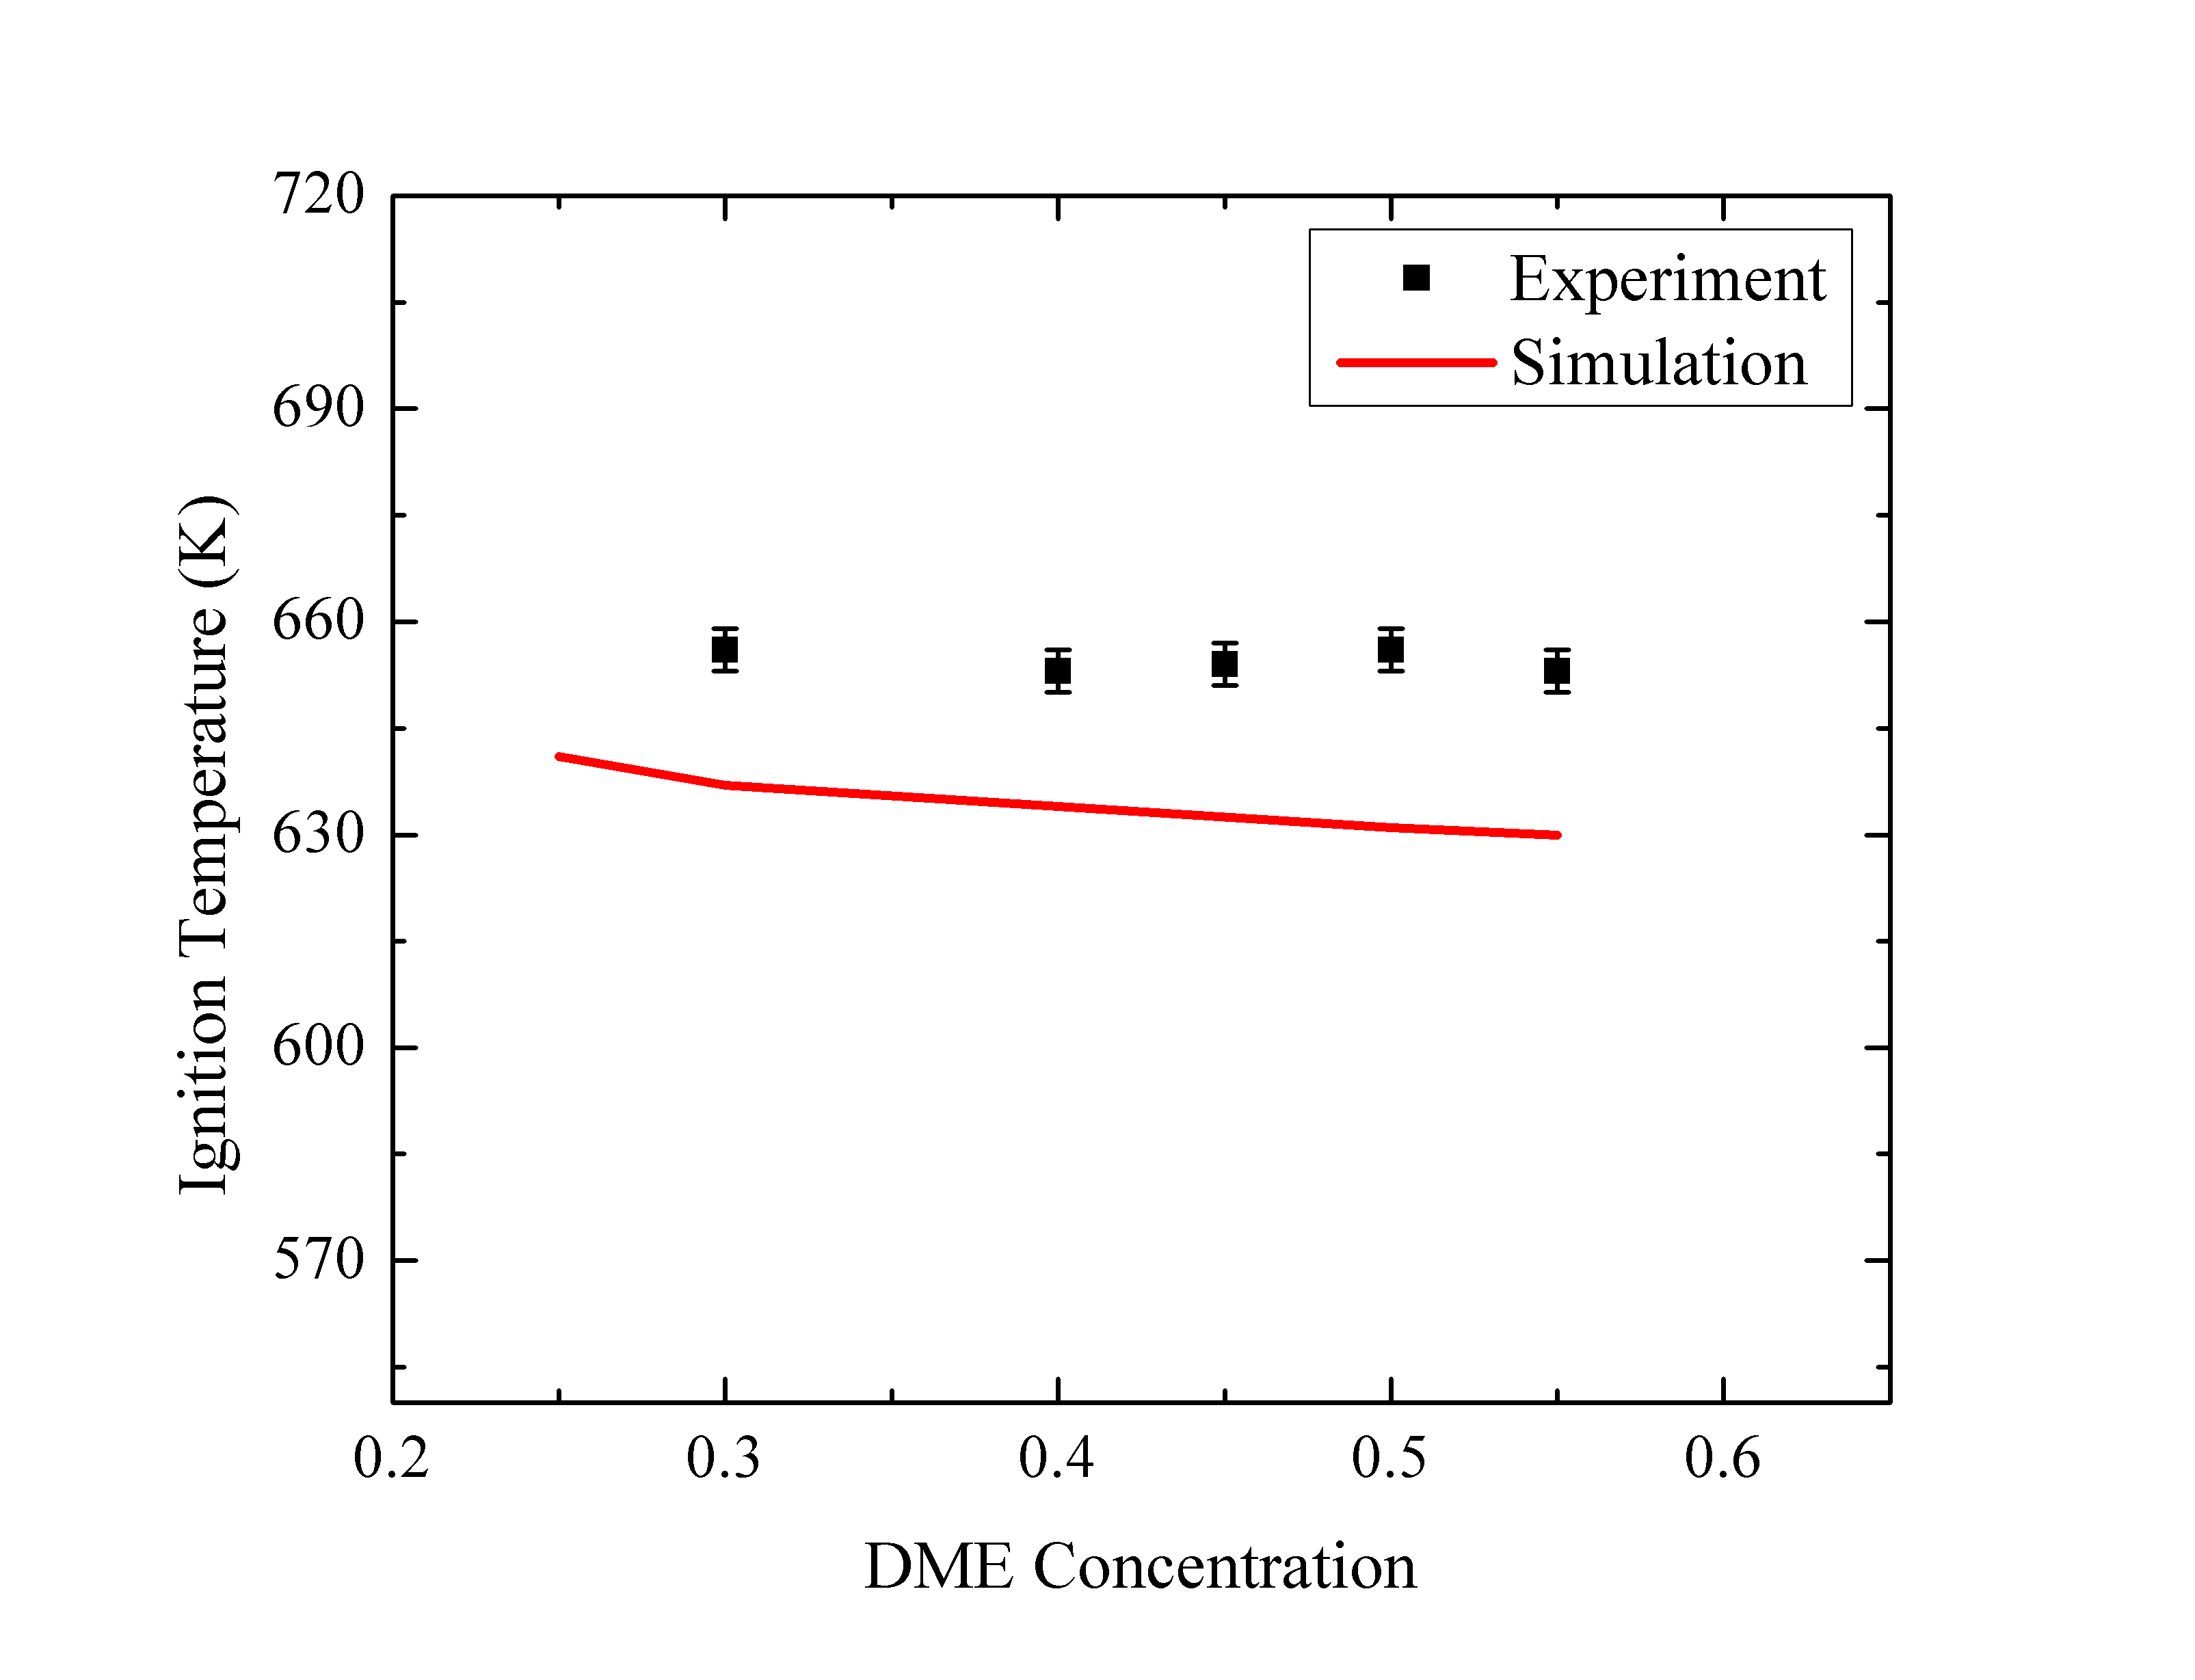
\includegraphics[width=0.6\textwidth]{Ign-Con.png}
  \normalsize
  \vspace{-0.1in}
  \caption{Ignition temperatures of various DME concentrations under the strain rate of $60$ /s.}
  \label{fig:Ign-Con}
\end{figure}


\section{Conclusions}        

Following our previous computational studies~\cite{law12,zhao13} that predicted the existence of low-temperature, NTC-affected, weakly burning diffusion flames in the counterflow, we have now successfully provided experimental substantiation of the existence of such flames.  In particular, the filtered PMT imaging demonstrated the presence of the signature HCHO chemiluminescence in the counterflow of heated air stream against nitrogen-diluted DME, while sensitive infrared imaging determined the corresponding ignition temperature.  Extensive experimentation then demonstrated that the low-temperature reactivity is enhanced with increasing air temperature, decreasing strain rate of the flow, and is insensitive to the DME concentrations.  Parallel computation substantiated the experimental results, and further corroborated the essential NTC chemistry governing the observed phenomena.

\section*{Acknowledgments}
This work was supported by the Combustion Energy Frontier Research Center, an Energy Frontier Research Center funded by the US Department of Energy, Office of Basic Energy Sciences under Award Number DE-SC0001198.

\section*{References}
\bibliographystyle{elsarticle-num-CNF}
\bibliography{NTC}

\renewcommand{\thefigure}{\arabic{figure}}
\renewcommand{\thetable}{\arabic{table}}

\end{document}


\chapter{Flame Dynamics at Engine Conditions}\label{ch:dynamics}

In this chapter, laminar nonpremixed coflow flame dynamics are studied computationally at elevated temperatures and pressures to activate autoignition.  Realizing practical engines work under turbulent and autoignitive conditions with unsteadiness in the inlet flows, the work presented in this disseration starts with steady laminar flow and then goes to unsteady laminar flow, gradually adding flow complexities to bridge laminar and turbulent studies.  Lifted flame stabilization at elevated temperatures and pressures is first presented to elucidate the role of autoignition in flame stabilization in addition to the traditional tribrachial flame stabilization.  Responsible for the first stage autoignition and heat release, the role of low-temperature chemistry, presented in Chapter~\ref{ch:NTC}, is investigated.  The thermal and chemical structures of the lifted flame are described with heat release and selected species profiles.  The evolution of the controlling chemical pathways are subsequently identified with Chemical Explosive Mode Analysis (CEMA) and the stabilization mechanism determined with Lagrangian Flamelet Analysis (LFA).  Different stabilization mechanisms are identified, and a regime diagram is proposed to demonstrate the shift of the stabilization mechanism as flow condition varies.  The complexity of unsteadiness is then added to the investigated problem by examining flame dynamics in an oscillating flow.  Consequently, the chemistry-transport coupling effects on the shift of combustion modes in oscillating flows under autoignitive conditions are elucidated.

\section{Computational Details} \label{sec:dynamics-computation}

The flow configuration is an axisymmetric DME stream at $300$ K in a heated coflow of air at $30$ atmospheres.  The fuel nozzle diameter $D$ is $0.8$ mm, and the fuel and air are initially separated with an adiabatic, no-slip wall with thickness $D/20$.  The schematic of this coflow configuration is provided in Fig.~\ref{fig:coflow}.  The coflow outer boundary is specified as an adiabatic slip wall, and its diameter is large enough such that increasing the width of the domain does not influence the computation.  Uniform inlet velocities were specified for both fuel and air streams to establish lifted flames.  For the unsteady estabilishment of the flame, a convective outflow is utilized at the outlet boundary, which simplifies to a Neumann condition for the steady problem.

\begin{figure}[t]
  \centering
  \scriptsize
  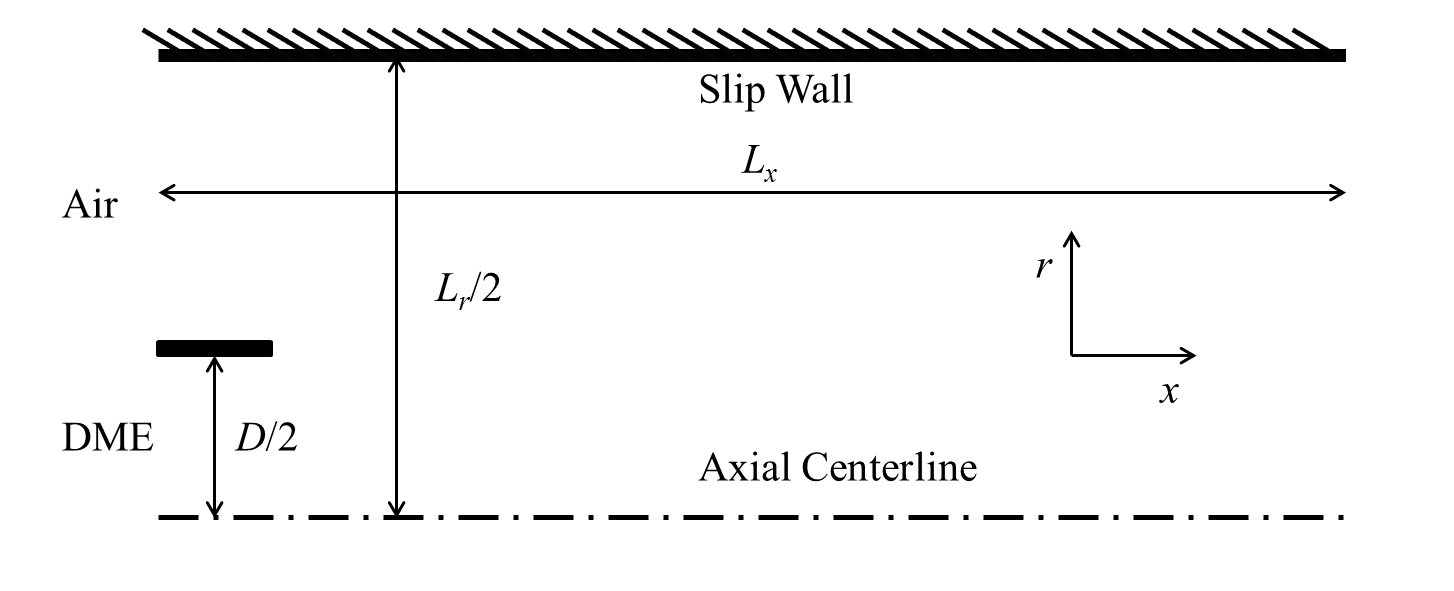
\includegraphics[width=1.0\textwidth]{ch-dynamics/coflow.png}
  \normalsize
  \caption{A schematic of the coflow configuration adopted in all of the steady and unsteady cases.}
  \label{fig:coflow}
\end{figure}

The flow field was initialized on a coarse mesh within a large domain.  At first, all the chemical source terms were set to zero until the nonreacting flow reached steady-state.  Chemical source terms were then activated; the mixture autoignited; and the flow field reached steady-state.  The domain was then truncated, and the mesh was refined to fully resolve the chemical structure.  All the results presented in Secs.~\ref{sec:dynamics-T} and~\ref{sec:dynamics-V} were obtained from the steady-state solutions.  

The Navier-Stokes equation with buoyancy in the streamwise direction and the conservation equations of mass, species, and temperature were solved.  The species diffusivities were determined from a constant, nonunity Lewis number.  The Lewis numbers for individual species were pre-calculated from a one-dimensional flamelet with the same boundary conditions and the mixture-averaged transport model and evaluated at the maximum temperature location.  The conserved scalar mixture fraction $Z$ was specified as unity and zero for the fuel jet and coflow at the inlet, respectively, and computed by solving its transport equation with unity Lewis number~\cite{pitsch98b}.  This definition of mixture fraction is consistent with the one used in the flamelet calculation in Sec.~\ref{sec:LFA}.

Dimethyl ether was chosen in this work, for it is a clean biofuel and one of the smallest hydrocarbons exhibiting NTC behavior.  The same skeletal mechanism~\cite{bhagatwala15} is utilized as in Chapter~\ref{ch:NTC}.

The low-Mach number formulation of the governing equations is solved using NGA, which is based on the numerical methods of Desjardins \emph{et al.}~\cite{desjardins08}.  The momentum and scalar equations are discretized with a second-order centered scheme and a third-order WENO scheme~\cite{liu94}, respectively, on a staggered mesh.  The iterative second-order semi-implicit Crank-Nicolson scheme of Pierce and Moin~\cite{pierce01} is adopted for temporal integration.  At each time step, the chemical source terms for the species and energy equations are evaluated independently from the transport terms using the CVODE package~\cite{cohen96}.

Uniform grids in the axial direction were adopted for the computations, and the grid spacing was set as $\Delta x = 2.2$ $\mu$m.  A nonuniform grid was used in the radial direction with a minimum spacing of $2.5$ $\mu$m to resolve the mixing layer corresponding to the separation wall and geometric progression stretch rates less than $3$\% towards both the centerline and the outer boundary.  The dimensions of and number of grid points in the computational domain for each computation are introduced in the following sections.

A grid convergence study was performed for the air temperature $800$ K case at $3.2$ m/s, for it has the most complex structure, which is discussed in the following sections.  As shown in Fig.~\ref{fig:convergence}, grid convergence was achieved for velocity, temperature, and species profiles.  Grid convergence was also verified for the air temperature $1100$ K case, which shows similar results and is therefore not shown here.  

\begin{figure}
  \centering
  \scriptsize
  \scalebox{1.5}{% GNUPLOT: LaTeX picture with Postscript
\begingroup
  \makeatletter
  \providecommand\color[2][]{%
    \GenericError{(gnuplot) \space\space\space\@spaces}{%
      Package color not loaded in conjunction with
      terminal option `colourtext'%
    }{See the gnuplot documentation for explanation.%
    }{Either use 'blacktext' in gnuplot or load the package
      color.sty in LaTeX.}%
    \renewcommand\color[2][]{}%
  }%
  \providecommand\includegraphics[2][]{%
    \GenericError{(gnuplot) \space\space\space\@spaces}{%
      Package graphicx or graphics not loaded%
    }{See the gnuplot documentation for explanation.%
    }{The gnuplot epslatex terminal needs graphicx.sty or graphics.sty.}%
    \renewcommand\includegraphics[2][]{}%
  }%
  \providecommand\rotatebox[2]{#2}%
  \@ifundefined{ifGPcolor}{%
    \newif\ifGPcolor
    \GPcolortrue
  }{}%
  \@ifundefined{ifGPblacktext}{%
    \newif\ifGPblacktext
    \GPblacktexttrue
  }{}%
  % define a \g@addto@macro without @ in the name:
  \let\gplgaddtomacro\g@addto@macro
  % define empty templates for all commands taking text:
  \gdef\gplbacktext{}%
  \gdef\gplfronttext{}%
  \makeatother
  \ifGPblacktext
    % no textcolor at all
    \def\colorrgb#1{}%
    \def\colorgray#1{}%
  \else
    % gray or color?
    \ifGPcolor
      \def\colorrgb#1{\color[rgb]{#1}}%
      \def\colorgray#1{\color[gray]{#1}}%
      \expandafter\def\csname LTw\endcsname{\color{white}}%
      \expandafter\def\csname LTb\endcsname{\color{black}}%
      \expandafter\def\csname LTa\endcsname{\color{black}}%
      \expandafter\def\csname LT0\endcsname{\color[rgb]{1,0,0}}%
      \expandafter\def\csname LT1\endcsname{\color[rgb]{0,1,0}}%
      \expandafter\def\csname LT2\endcsname{\color[rgb]{0,0,1}}%
      \expandafter\def\csname LT3\endcsname{\color[rgb]{1,0,1}}%
      \expandafter\def\csname LT4\endcsname{\color[rgb]{0,1,1}}%
      \expandafter\def\csname LT5\endcsname{\color[rgb]{1,1,0}}%
      \expandafter\def\csname LT6\endcsname{\color[rgb]{0,0,0}}%
      \expandafter\def\csname LT7\endcsname{\color[rgb]{1,0.3,0}}%
      \expandafter\def\csname LT8\endcsname{\color[rgb]{0.5,0.5,0.5}}%
    \else
      % gray
      \def\colorrgb#1{\color{black}}%
      \def\colorgray#1{\color[gray]{#1}}%
      \expandafter\def\csname LTw\endcsname{\color{white}}%
      \expandafter\def\csname LTb\endcsname{\color{black}}%
      \expandafter\def\csname LTa\endcsname{\color{black}}%
      \expandafter\def\csname LT0\endcsname{\color{black}}%
      \expandafter\def\csname LT1\endcsname{\color{black}}%
      \expandafter\def\csname LT2\endcsname{\color{black}}%
      \expandafter\def\csname LT3\endcsname{\color{black}}%
      \expandafter\def\csname LT4\endcsname{\color{black}}%
      \expandafter\def\csname LT5\endcsname{\color{black}}%
      \expandafter\def\csname LT6\endcsname{\color{black}}%
      \expandafter\def\csname LT7\endcsname{\color{black}}%
      \expandafter\def\csname LT8\endcsname{\color{black}}%
    \fi
  \fi
  \setlength{\unitlength}{0.0500bp}%
  \begin{picture}(3240.00,2520.00)%
    \gplgaddtomacro\gplbacktext{%
      \csname LTb\endcsname%
      \put(682,704){\makebox(0,0)[r]{\strut{} 0}}%
      \put(682,1092){\makebox(0,0)[r]{\strut{} 1}}%
      \put(682,1480){\makebox(0,0)[r]{\strut{} 2}}%
      \put(682,1868){\makebox(0,0)[r]{\strut{} 3}}%
      \put(682,2256){\makebox(0,0)[r]{\strut{} 4}}%
      \put(814,484){\makebox(0,0){\strut{} 0}}%
      \put(1220,484){\makebox(0,0){\strut{} 2}}%
      \put(1626,484){\makebox(0,0){\strut{} 4}}%
      \put(2031,484){\makebox(0,0){\strut{} 6}}%
      \put(2437,484){\makebox(0,0){\strut{} 8}}%
      \put(2843,484){\makebox(0,0){\strut{} 10}}%
      \put(176,1480){\rotatebox{-270}{\makebox(0,0){\strut{}\vspace{-28pt}$U$ [m/s]}}}%
      \put(1828,154){\makebox(0,0){\strut{}$x/D$}}%
      \put(1475,1170){\makebox(0,0)[l]{\strut{}Nominal}}%
      \put(1475,956){\makebox(0,0)[l]{\strut{}Coarser}}%
    }%
    \gplgaddtomacro\gplfronttext{%
      \csname LTb\endcsname%
      \put(2003,1176){\makebox(0,0)[r]{\strut{} }}%
      \csname LTb\endcsname%
      \put(2003,956){\makebox(0,0)[r]{\strut{} }}%
    }%
    \gplbacktext
    \put(0,0){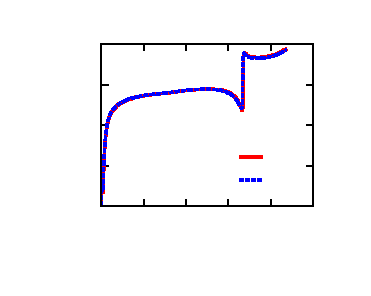
\includegraphics{ch-dynamics/conv_zst_U}}%
    \gplfronttext
  \end{picture}%
\endgroup
}
  \scalebox{1.5}{% GNUPLOT: LaTeX picture with Postscript
\begingroup
  \makeatletter
  \providecommand\color[2][]{%
    \GenericError{(gnuplot) \space\space\space\@spaces}{%
      Package color not loaded in conjunction with
      terminal option `colourtext'%
    }{See the gnuplot documentation for explanation.%
    }{Either use 'blacktext' in gnuplot or load the package
      color.sty in LaTeX.}%
    \renewcommand\color[2][]{}%
  }%
  \providecommand\includegraphics[2][]{%
    \GenericError{(gnuplot) \space\space\space\@spaces}{%
      Package graphicx or graphics not loaded%
    }{See the gnuplot documentation for explanation.%
    }{The gnuplot epslatex terminal needs graphicx.sty or graphics.sty.}%
    \renewcommand\includegraphics[2][]{}%
  }%
  \providecommand\rotatebox[2]{#2}%
  \@ifundefined{ifGPcolor}{%
    \newif\ifGPcolor
    \GPcolortrue
  }{}%
  \@ifundefined{ifGPblacktext}{%
    \newif\ifGPblacktext
    \GPblacktexttrue
  }{}%
  % define a \g@addto@macro without @ in the name:
  \let\gplgaddtomacro\g@addto@macro
  % define empty templates for all commands taking text:
  \gdef\gplbacktext{}%
  \gdef\gplfronttext{}%
  \makeatother
  \ifGPblacktext
    % no textcolor at all
    \def\colorrgb#1{}%
    \def\colorgray#1{}%
  \else
    % gray or color?
    \ifGPcolor
      \def\colorrgb#1{\color[rgb]{#1}}%
      \def\colorgray#1{\color[gray]{#1}}%
      \expandafter\def\csname LTw\endcsname{\color{white}}%
      \expandafter\def\csname LTb\endcsname{\color{black}}%
      \expandafter\def\csname LTa\endcsname{\color{black}}%
      \expandafter\def\csname LT0\endcsname{\color[rgb]{1,0,0}}%
      \expandafter\def\csname LT1\endcsname{\color[rgb]{0,1,0}}%
      \expandafter\def\csname LT2\endcsname{\color[rgb]{0,0,1}}%
      \expandafter\def\csname LT3\endcsname{\color[rgb]{1,0,1}}%
      \expandafter\def\csname LT4\endcsname{\color[rgb]{0,1,1}}%
      \expandafter\def\csname LT5\endcsname{\color[rgb]{1,1,0}}%
      \expandafter\def\csname LT6\endcsname{\color[rgb]{0,0,0}}%
      \expandafter\def\csname LT7\endcsname{\color[rgb]{1,0.3,0}}%
      \expandafter\def\csname LT8\endcsname{\color[rgb]{0.5,0.5,0.5}}%
    \else
      % gray
      \def\colorrgb#1{\color{black}}%
      \def\colorgray#1{\color[gray]{#1}}%
      \expandafter\def\csname LTw\endcsname{\color{white}}%
      \expandafter\def\csname LTb\endcsname{\color{black}}%
      \expandafter\def\csname LTa\endcsname{\color{black}}%
      \expandafter\def\csname LT0\endcsname{\color{black}}%
      \expandafter\def\csname LT1\endcsname{\color{black}}%
      \expandafter\def\csname LT2\endcsname{\color{black}}%
      \expandafter\def\csname LT3\endcsname{\color{black}}%
      \expandafter\def\csname LT4\endcsname{\color{black}}%
      \expandafter\def\csname LT5\endcsname{\color{black}}%
      \expandafter\def\csname LT6\endcsname{\color{black}}%
      \expandafter\def\csname LT7\endcsname{\color{black}}%
      \expandafter\def\csname LT8\endcsname{\color{black}}%
    \fi
  \fi
  \setlength{\unitlength}{0.0500bp}%
  \begin{picture}(3600.00,2520.00)%
    \gplgaddtomacro\gplbacktext{%
      \csname LTb\endcsname%
      \put(1078,704){\makebox(0,0)[r]{\strut{} 600}}%
      \put(1078,1014){\makebox(0,0)[r]{\strut{} 1000}}%
      \put(1078,1325){\makebox(0,0)[r]{\strut{} 1400}}%
      \put(1078,1635){\makebox(0,0)[r]{\strut{} 1800}}%
      \put(1078,1946){\makebox(0,0)[r]{\strut{} 2200}}%
      \put(1078,2256){\makebox(0,0)[r]{\strut{} 2600}}%
      \put(1210,484){\makebox(0,0){\strut{} 0}}%
      \put(1609,484){\makebox(0,0){\strut{} 2}}%
      \put(2007,484){\makebox(0,0){\strut{} 4}}%
      \put(2406,484){\makebox(0,0){\strut{} 6}}%
      \put(2804,484){\makebox(0,0){\strut{} 8}}%
      \put(3203,484){\makebox(0,0){\strut{} 10}}%
      \put(176,1480){\rotatebox{-270}{\makebox(0,0){\strut{}\vspace{-48pt}$T$ [K]}}}%
      \put(2206,154){\makebox(0,0){\strut{}$x/D$}}%
      \put(1459,2023){\makebox(0,0)[l]{\strut{}Nominal}}%
      \put(1459,1790){\makebox(0,0)[l]{\strut{}Coarser}}%
    }%
    \gplgaddtomacro\gplfronttext{%
      \csname LTb\endcsname%
      \put(1871,2037){\makebox(0,0)[r]{\strut{} }}%
      \csname LTb\endcsname%
      \put(1871,1817){\makebox(0,0)[r]{\strut{} }}%
    }%
    \gplbacktext
    \put(0,0){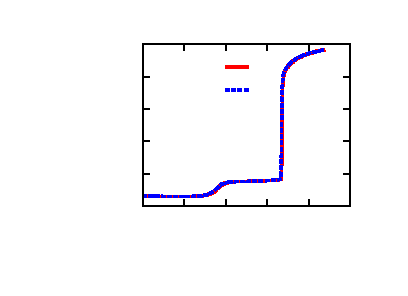
\includegraphics{conv_zst_T}}%
    \gplfronttext
  \end{picture}%
\endgroup
}
  \scalebox{1.5}{% GNUPLOT: LaTeX picture with Postscript
\begingroup
  \makeatletter
  \providecommand\color[2][]{%
    \GenericError{(gnuplot) \space\space\space\@spaces}{%
      Package color not loaded in conjunction with
      terminal option `colourtext'%
    }{See the gnuplot documentation for explanation.%
    }{Either use 'blacktext' in gnuplot or load the package
      color.sty in LaTeX.}%
    \renewcommand\color[2][]{}%
  }%
  \providecommand\includegraphics[2][]{%
    \GenericError{(gnuplot) \space\space\space\@spaces}{%
      Package graphicx or graphics not loaded%
    }{See the gnuplot documentation for explanation.%
    }{The gnuplot epslatex terminal needs graphicx.sty or graphics.sty.}%
    \renewcommand\includegraphics[2][]{}%
  }%
  \providecommand\rotatebox[2]{#2}%
  \@ifundefined{ifGPcolor}{%
    \newif\ifGPcolor
    \GPcolortrue
  }{}%
  \@ifundefined{ifGPblacktext}{%
    \newif\ifGPblacktext
    \GPblacktexttrue
  }{}%
  % define a \g@addto@macro without @ in the name:
  \let\gplgaddtomacro\g@addto@macro
  % define empty templates for all commands taking text:
  \gdef\gplbacktext{}%
  \gdef\gplfronttext{}%
  \makeatother
  \ifGPblacktext
    % no textcolor at all
    \def\colorrgb#1{}%
    \def\colorgray#1{}%
  \else
    % gray or color?
    \ifGPcolor
      \def\colorrgb#1{\color[rgb]{#1}}%
      \def\colorgray#1{\color[gray]{#1}}%
      \expandafter\def\csname LTw\endcsname{\color{white}}%
      \expandafter\def\csname LTb\endcsname{\color{black}}%
      \expandafter\def\csname LTa\endcsname{\color{black}}%
      \expandafter\def\csname LT0\endcsname{\color[rgb]{1,0,0}}%
      \expandafter\def\csname LT1\endcsname{\color[rgb]{0,1,0}}%
      \expandafter\def\csname LT2\endcsname{\color[rgb]{0,0,1}}%
      \expandafter\def\csname LT3\endcsname{\color[rgb]{1,0,1}}%
      \expandafter\def\csname LT4\endcsname{\color[rgb]{0,1,1}}%
      \expandafter\def\csname LT5\endcsname{\color[rgb]{1,1,0}}%
      \expandafter\def\csname LT6\endcsname{\color[rgb]{0,0,0}}%
      \expandafter\def\csname LT7\endcsname{\color[rgb]{1,0.3,0}}%
      \expandafter\def\csname LT8\endcsname{\color[rgb]{0.5,0.5,0.5}}%
    \else
      % gray
      \def\colorrgb#1{\color{black}}%
      \def\colorgray#1{\color[gray]{#1}}%
      \expandafter\def\csname LTw\endcsname{\color{white}}%
      \expandafter\def\csname LTb\endcsname{\color{black}}%
      \expandafter\def\csname LTa\endcsname{\color{black}}%
      \expandafter\def\csname LT0\endcsname{\color{black}}%
      \expandafter\def\csname LT1\endcsname{\color{black}}%
      \expandafter\def\csname LT2\endcsname{\color{black}}%
      \expandafter\def\csname LT3\endcsname{\color{black}}%
      \expandafter\def\csname LT4\endcsname{\color{black}}%
      \expandafter\def\csname LT5\endcsname{\color{black}}%
      \expandafter\def\csname LT6\endcsname{\color{black}}%
      \expandafter\def\csname LT7\endcsname{\color{black}}%
      \expandafter\def\csname LT8\endcsname{\color{black}}%
    \fi
  \fi
  \setlength{\unitlength}{0.0500bp}%
  \begin{picture}(3744.00,2520.00)%
    \gplgaddtomacro\gplbacktext{%
      \csname LTb\endcsname%
      \put(1210,704){\makebox(0,0)[r]{\strut{} 0}}%
      \put(1210,1014){\makebox(0,0)[r]{\strut{} 0.002}}%
      \put(1210,1325){\makebox(0,0)[r]{\strut{} 0.004}}%
      \put(1210,1635){\makebox(0,0)[r]{\strut{} 0.006}}%
      \put(1210,1946){\makebox(0,0)[r]{\strut{} 0.008}}%
      \put(1210,2256){\makebox(0,0)[r]{\strut{} 0.01}}%
      \put(1342,484){\makebox(0,0){\strut{} 0}}%
      \put(1743,484){\makebox(0,0){\strut{} 2}}%
      \put(2144,484){\makebox(0,0){\strut{} 4}}%
      \put(2545,484){\makebox(0,0){\strut{} 6}}%
      \put(2946,484){\makebox(0,0){\strut{} 8}}%
      \put(3347,484){\makebox(0,0){\strut{} 10}}%
      \put(176,1480){\rotatebox{-270}{\makebox(0,0){\strut{}\vspace{-52pt}$Y_{\rm H_2O_2}$}}}%
      \put(2344,154){\makebox(0,0){\strut{}$x/D$}}%
      \put(1593,2023){\makebox(0,0)[l]{\strut{}Nominal}}%
      \put(1593,1790){\makebox(0,0)[l]{\strut{}Coarser}}%
    }%
    \gplgaddtomacro\gplfronttext{%
      \csname LTb\endcsname%
      \put(2035,2022){\makebox(0,0)[r]{\strut{} }}%
      \csname LTb\endcsname%
      \put(2035,1802){\makebox(0,0)[r]{\strut{} }}%
    }%
    \gplbacktext
    \put(0,0){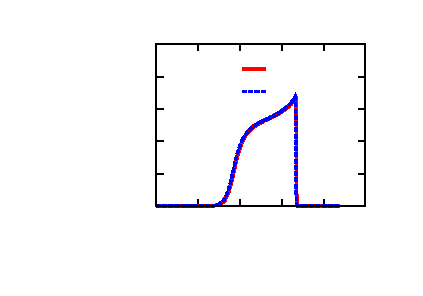
\includegraphics{conv_zst_H2O2}}%
    \gplfronttext
  \end{picture}%
\endgroup
}
  \caption{Velocity, temperature, and H$_2$O$_2$ profiles along $Z_{\rm st}$ on the nominal and two times coarser (in each direction) meshes for an air temperature of $800$ K.}
  \label{fig:convergence}
\end{figure}

\section{Flame Stabilization: Boundary Temperature Effects}\label{sec:dynamics-T}

In this section, the effect of boundary temperature on flame stabilization is investigated.  Therefore, in all cases studied in this section, the boundary velocities of the DME jet as well as the coflow air are fixed at $3.2$ m/s.  Conversely, the temperatures of the heated air coflow are $700$, $800$, $900$, and $1100$ K.  The dimensions of and number of grid points in the computational domain for each computation are summarized in Table~\ref{table:domain_T}. 

\begin{table*}
  \caption{Computational domain and number of grid points for steady cases with the same flow velocities but different boundary temperatures.}
  \label{table:domain_T}
  \centering
  \normalsize
  \resizebox{0.8\textwidth}{!}{
  \begin{tabular}{lc*{3}{c}}
    \hline
    Coflow Temperature [K]& $700$  & $800$  & $900$  & $1100$   \\
    \hline
    $L_x$ [mm]& $28$ & $7$ & $3.5$ & $3$\\
    $L_r$ [mm]& $6$ & $3.9$ & $3.9$  & $6$\\
    $N_x$ & $12290$ & $3072$ & $1536$  & $1282$\\
    $N_r$ & $192$ & $176$ & $176$  & $192$\\
    \hline
   \end{tabular}
}
\end{table*}

\subsection{Thermal and Chemical Structure} \label{sec:dynamcis-structure_T}

To visualize the flame structures, the heat release rate profiles for the four cases ($700$, $800$, $900$, and $1100$ K) are shown in Fig.~\ref{fig:dynamics-HRR_T}.  Qualitatively, the most upstream point on the largest heat release contour (the leading point), colored by red, will be referred to as the stabilization point.  

\begin{figure}[t]
  \centering
  \scriptsize
  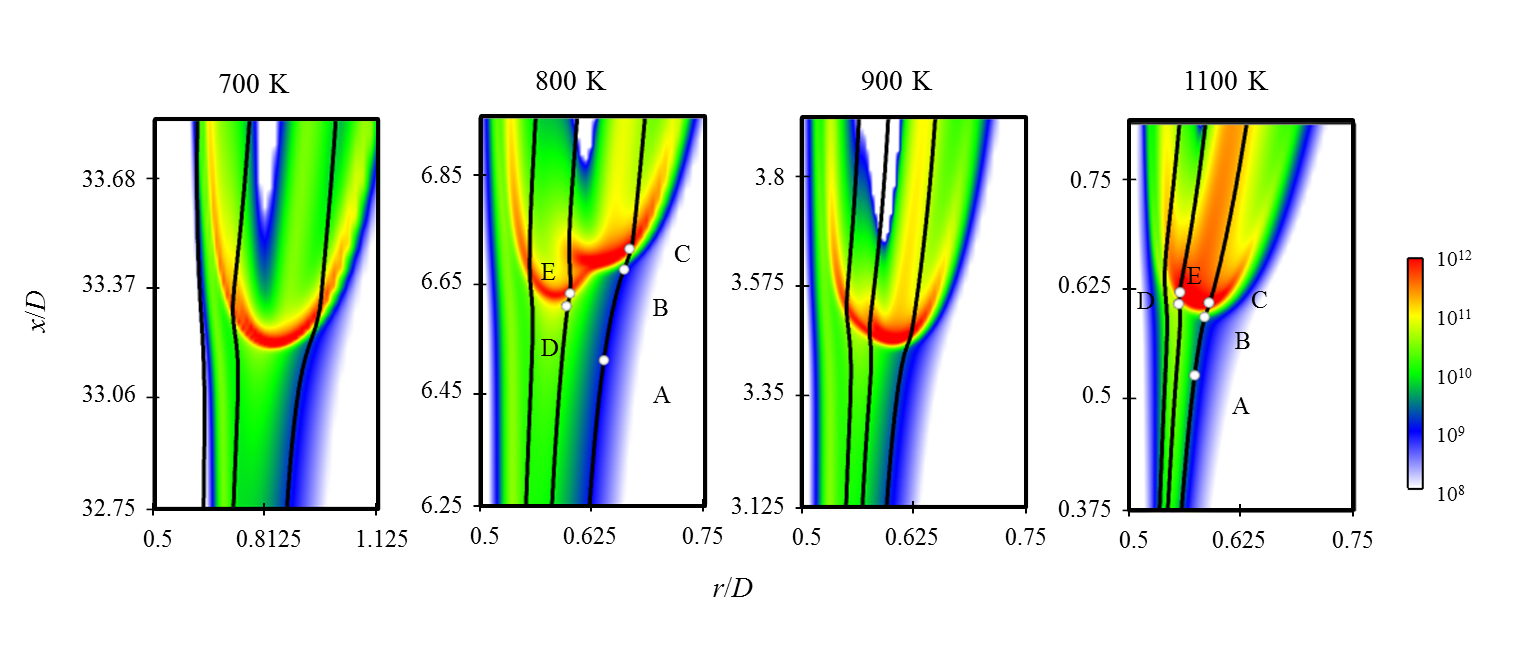
\includegraphics[width=1.0\textwidth]{ch-dynamics/HRR_T.png}
  \normalsize
  \caption{Heat release rate [J/m$^3$-s] profiles for the steady cases with the same flow velocities but different boundary temperatures.  The iso-contours of $Z_{\rm st}$, $Z = 0.2$, and $Z = 0.3$ are outlined from right to left in solid lines, respectively.  The CEMA sampling points at $800$ and $1100$ K are indicated along the iso-contours.}
  \label{fig:dynamics-HRR_T}
\end{figure}

At $700$ K, a tribrachial thermal structure is observed, and the stabilization point is located around $Z = 0.15$, which is richer than the triple point, where the three branches intersect.  Moreover, compared to the classical triple flame structure, the middle heat release rate branch, corresponding to the nonpremixed flame, is significantly weaker than the other two branches.  

At $800$ K, the stabilization point is not located on the tribrachial structure any more.  Instead, it is located near $Z = 0.23$ and connects two trailing heat release branches, where a tribrachial flame structure is attached to the leaner branch (LB) of the bibrachial reacting front.  A schematic of the structure is shown in Fig.~\ref{fig:schematic_800}.

\begin{figure}[t]
  \centering
  \scriptsize
  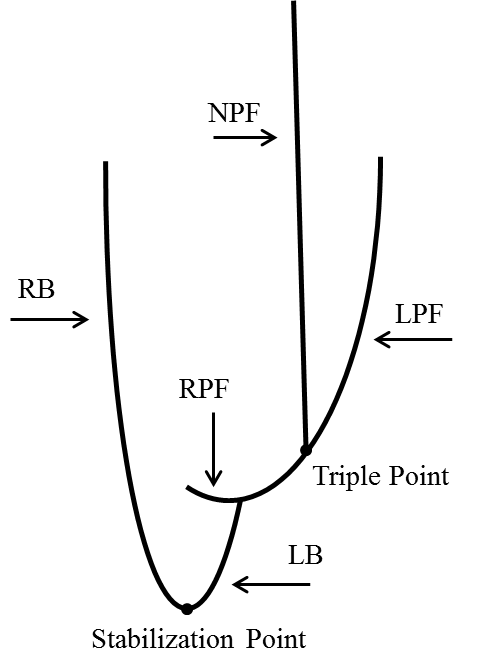
\includegraphics[width=0.4\textwidth]{ch-dynamics/schematic_800.png}
  \normalsize
  \caption{A schematic of the thermal structure of the $800$ K case.  LPF, RPF, and NPF denotes the lean premixed, rich premixed, and nonpremixed flame branches on the tribrachial structure, respectively.  LB and RB denotes the leaner and richer branches of the reacting front, respectively.}
  \label{fig:schematic_800}
\end{figure}

As the air boundary temperature increases to $900$ K, the stabilization point shifts back to $Z = 0.14$.  Moreover, a long trailing branch at richer mixture fraction is attached to the main tribrachial structure, resulting in a tetrabrachial structure.  Compared with the structure shown in the $800$ K case, the main tribrachial structure stabilizes further upstream, for it depends less on the radical accumulation ahead of the flame.  Therefore, it catches up with the reacting front at richer mixture fraction, and they merge into the apparent tetrabrachial structure.

A further increase in the boundary temperature results in a structure that is very similar to the classical triple flame, except for the fact that there is also heat release ahead of the stabilization point at $Z = 0.13$.  Some of the multibrachial structures were also observed by Krisman \emph{et al.}~\cite{krisman15}, using different definitions for branches, and it was concluded that the autoignition chemistry could affect the flame structure and the stabilization mechanism.  

To first qualitatively demonstrate the chemical structure of the flame, selected species profiles were examined, shown in Figs.~\ref{fig:OH_T} to~\ref{fig:H2O2_T}.  The methoxymethylperoxy radical (CH$_3$OCH$_2$O$_2$) and hydroxyl radical (OH) were chosen as indicators of low and high-temperature chemistry, respectively.  The hydroperoxyl radical (HO$_2$) and hydrogen peroxide (H$_2$O$_2$) were chosen, for they form in the preheat zone of a flame or before autoignition but quickly vanish in the post flame zone or after ignition~\cite{yoo09}.

For all four cases, similar profiles can be seen for some species.  First, low-temperature chemistry, indicated by the CH$_3$OCH$_2$O$_2$ radical, is found to be important at richer mixture fractions, where the temperature is also lower.  Second, the OH radical peaks at and downstream of the maximum heat release locations and correlates well with the tribrachial structure shown in the heat release rate profiles, indicating the presence of high-temperature chemistry.  Third, the HO$_2$ mass fraction peaks in a thin region.  Compared with the heat release rate contours, this thin region outlines the flame front and the reactive mixture at the rich mixture fractions and indicates the importance of the exothermic three-body recombination reaction H + O$_2$ + M $\Longleftrightarrow$ HO$_2$ + M.

However, there are also differences in the chemical structure among the different cases.  For example, for the $800$ and $900$ K cases, another OH local maxima, which is two orders of magnitudes smaller than the peak value on the tribrachial structure, appears at richer mixture fractions, immediately downstream of where the CH$_3$OCH$_2$O$_2$ radical and H$_2$O$_2$ disappear, indicating autoignition.  Moreover, more pronounced differences between the three lower boundary temperature cases and the $1100$ K case are shown in the H$_2$O$_2$ profiles: for the lower boundary temperature cases, H$_2$O$_2$ accumulates along the mixture fraction iso-contours  until it decomposes in the flame region, while, for the $1100$ K case, the H$_2$O$_2$ accumulation is an order of magnitude lower, due to the reduced residence time from the nozzle exit to the flame base.

\begin{figure}[t]
  \centering
  \scriptsize
  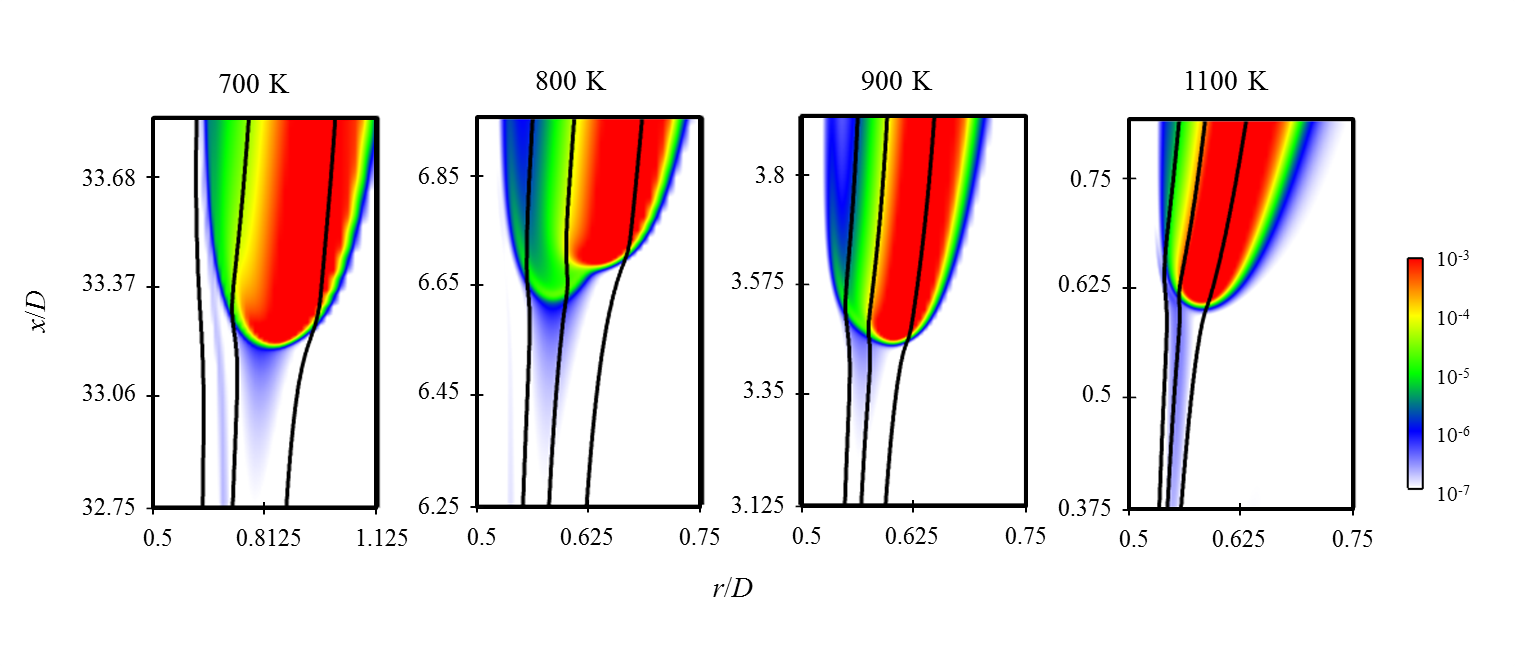
\includegraphics[width=1.0\textwidth]{ch-dynamics/OH_T.png}
  \normalsize
  \caption{Hydroxyl (OH) radical mass fraction profiles for the steady cases with the same flow velocities but different boundary temperatures.  The mixture fraction iso-contours are the same as in Fig.~\ref{fig:dynamics-HRR_T}.}
  \label{fig:OH_T}
\end{figure}

\begin{figure}[t]
  \centering
  \scriptsize
  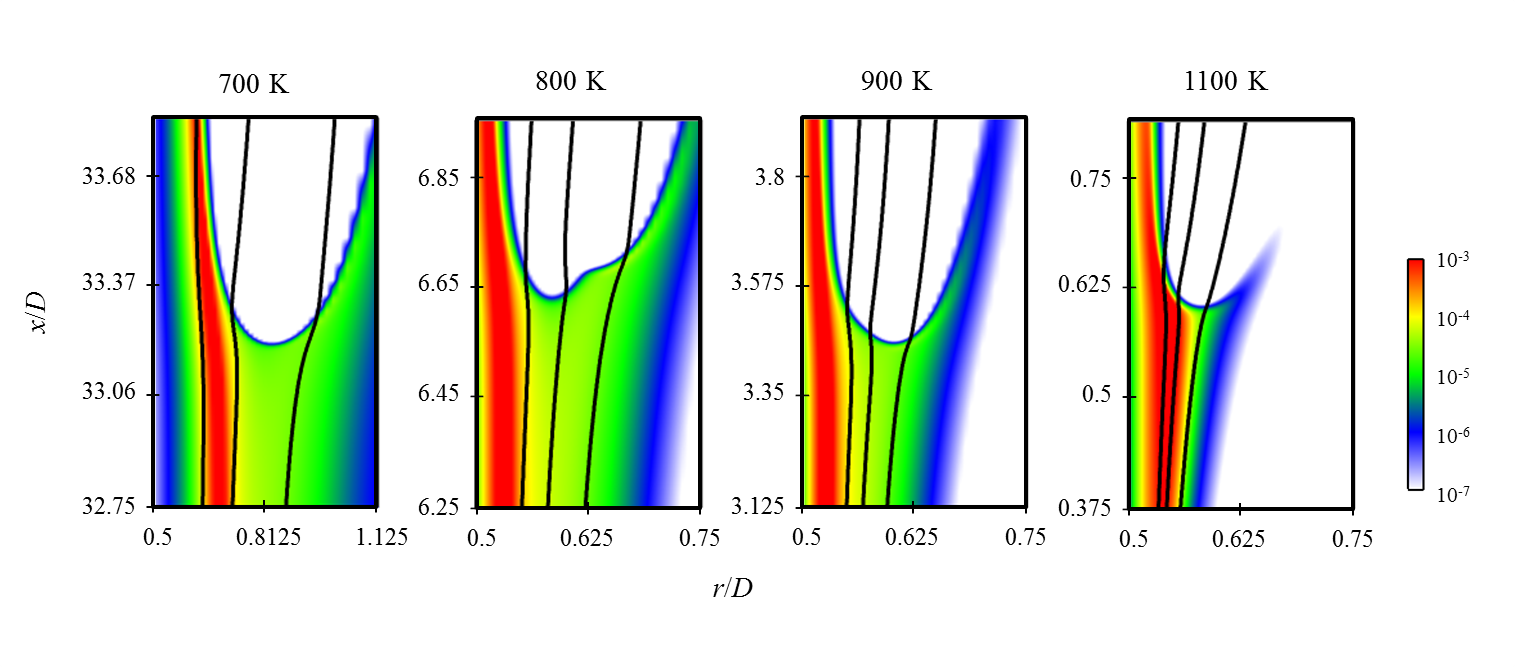
\includegraphics[width=1.0\textwidth]{ch-dynamics/RO2_T.png}
  \normalsize
  \caption{Methoxymethylperoxy (CH$_3$OCH$_2$O$_2$) radical mass fraction profiles for the steady cases with the same flow velocities but different boundary temperatures.  The mixture fraction iso-contours are the same as in Fig.~\ref{fig:dynamics-HRR_T}.}
  \label{fig:RO2_T}
\end{figure}

\begin{figure}[t]
  \centering
  \scriptsize
  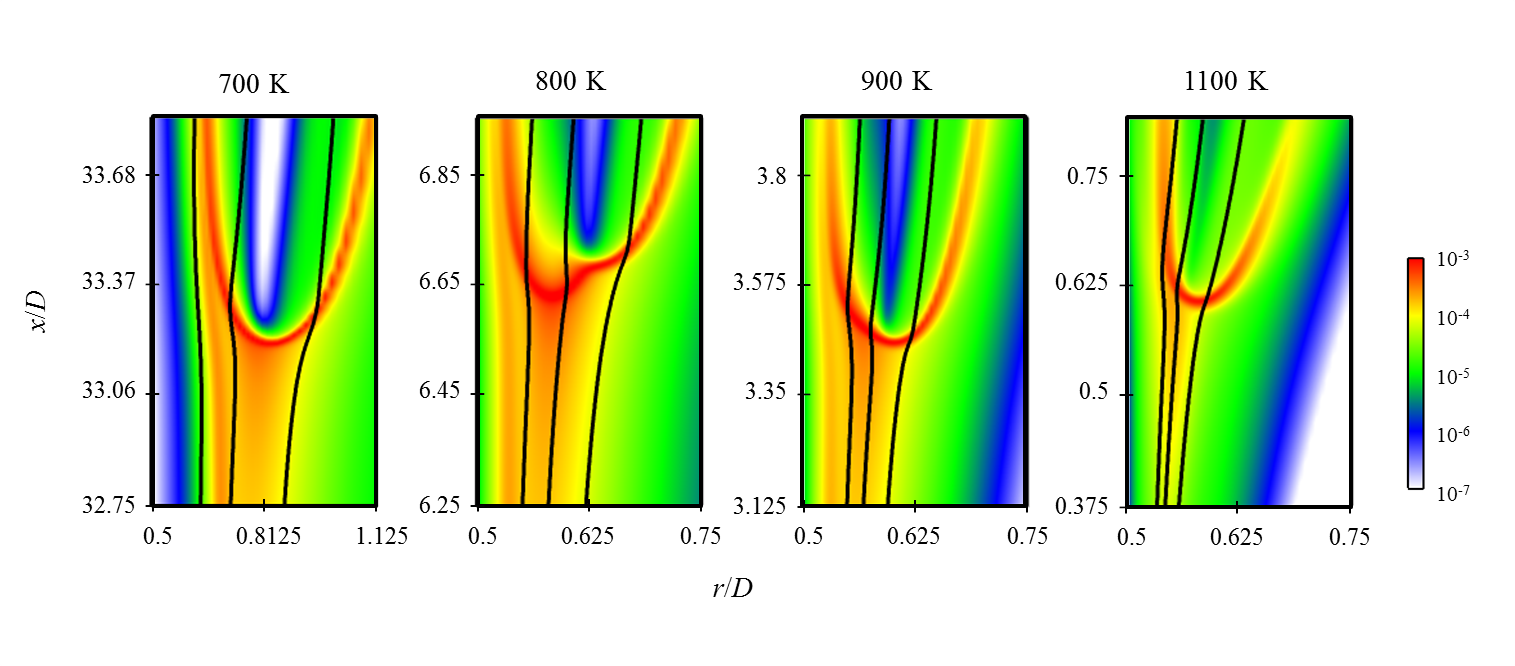
\includegraphics[width=1.0\textwidth]{ch-dynamics/HO2_T.png}
  \normalsize
  \caption{Hydroperoxyl (HO$_2$) radical mass fraction profiles for the steady cases with the same flow velocities but different boundary temperatures.  The mixture fraction iso-contours are the same as in Fig.~\ref{fig:dynamics-HRR_T}.}
  \label{fig:HO2_T}
\end{figure}

\begin{figure}[t]
  \centering
  \scriptsize
  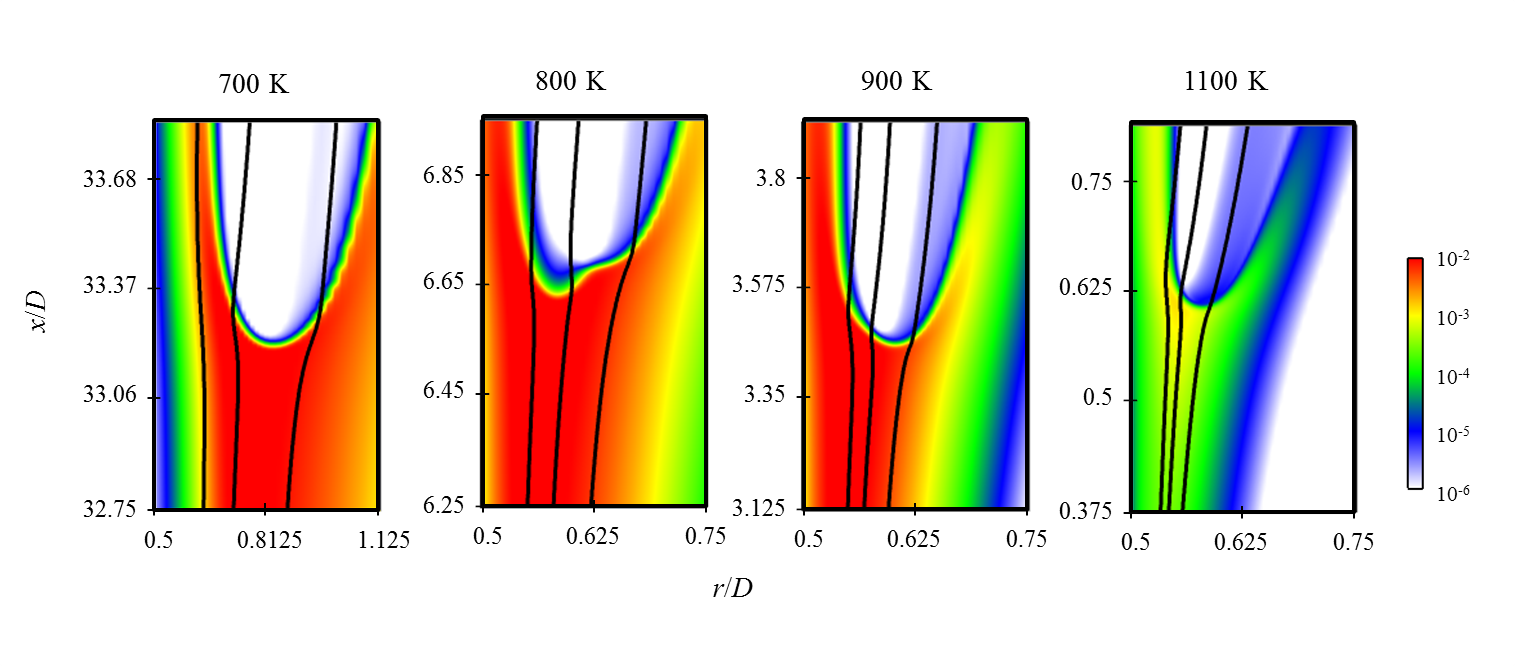
\includegraphics[width=1.0\textwidth]{ch-dynamics/H2O2_T.png}
  \normalsize
  \caption{Hydrogen peroxide (H$_2$O$_2$) mass fraction profiles for the steady cases with the same flow velocities but different boundary temperatures.  The mixture fraction iso-contours are the same as in Fig.~\ref{fig:dynamics-HRR_T}.}
  \label{fig:H2O2_T}
\end{figure}

\subsection{Computational Diagnostics and Analysis} \label{sec:diagnostics}

The above heat release rate and species profiles demonstrate the thermal and chemical structure of the reacting fronts at different boundary temperatures.  However, more detailed computational diagnostics and analysis are needed to further demonstrate the controlling chemistry and the stabilization mechanism.

\subsubsection{Chemical Explosive Mode Analysis}
In addition to the analysis based on selected species profiles, Chemical Explosive Mode Analysis (CEMA)~\cite{lu10,shan12} was conducted to identify the controlling chemistry in these complex reacting flows.  Briefly, local species concentrations and temperature are sampled from the two-dimensional computation and input into CEMA to evaluate the eigenvalues of the Jacobian matrix ($K + 1$ by $K + 1$, where $K$ is the number of species) of the chemical source terms.  The eigenmode associated with the eigenvalue $\lambda_{\rm e}$, which has the largest real part among all the eigenvalues, is defined as a chemical explosive mode, if

\begin{equation}
\rm{Re}(\lambda_{\rm e}) > 0, \lambda_{\rm e} = \mathbf{b_{\rm e}J_{\omega}a_{\rm e}},
\end{equation}
where $\mathbf{b_{\rm e}}$ and $\mathbf{a_{\rm e}}$ are the left and right eigenvectors, respectively, associated with $\lambda_{\rm e}$, and $\mathbf{J_{\omega}}$ is the chemical Jacobian matrix.  The existence of the chemical explosive mode indicates the propensity of local mixture autoignition given an isolated, adiabatic, and constant volume environment.  Furthermore, the detailed chemical reactions that contribute to the chemical explosive mode can be quantified by the explosion participation index:

\begin{equation}
\mathbf{PI} = \frac{|(\mathbf{b_{\rm e}} \cdot \mathbf{S}) \otimes \mathbf{R}|}{sum(|(\mathbf{b_{\rm e}} \cdot \mathbf{S}) \otimes \mathbf{R}|)},
\end{equation}
where $\mathbf{S}$ is the stoichiometric coefficient matrix, $\mathbf{R}$ is the vector of the net rates for the reactions, and $\otimes$ denotes elementwise multiplication of two vectors.  

The dominant reactions at representative locations, such as those upstream and near the flame base, are identified, based on the explosive mode and participation index.  For each case, the local species concentrations and temperature were sampled along the $Z_{\rm st}$, $Z = 0.2$, and $Z = 0.3$ iso-contours, as indicated in Fig.~\ref{fig:dynamics-HRR_T}, and processed by CEMA to demonstrate the evolution of the dominant reactions.

\begin{figure}
  \centering
  \scriptsize
  % GNUPLOT: LaTeX picture with Postscript
\begingroup
  \makeatletter
  \providecommand\color[2][]{%
    \GenericError{(gnuplot) \space\space\space\@spaces}{%
      Package color not loaded in conjunction with
      terminal option `colourtext'%
    }{See the gnuplot documentation for explanation.%
    }{Either use 'blacktext' in gnuplot or load the package
      color.sty in LaTeX.}%
    \renewcommand\color[2][]{}%
  }%
  \providecommand\includegraphics[2][]{%
    \GenericError{(gnuplot) \space\space\space\@spaces}{%
      Package graphicx or graphics not loaded%
    }{See the gnuplot documentation for explanation.%
    }{The gnuplot epslatex terminal needs graphicx.sty or graphics.sty.}%
    \renewcommand\includegraphics[2][]{}%
  }%
  \providecommand\rotatebox[2]{#2}%
  \@ifundefined{ifGPcolor}{%
    \newif\ifGPcolor
    \GPcolortrue
  }{}%
  \@ifundefined{ifGPblacktext}{%
    \newif\ifGPblacktext
    \GPblacktexttrue
  }{}%
  % define a \g@addto@macro without @ in the name:
  \let\gplgaddtomacro\g@addto@macro
  % define empty templates for all commands taking text:
  \gdef\gplbacktext{}%
  \gdef\gplfronttext{}%
  \makeatother
  \ifGPblacktext
    % no textcolor at all
    \def\colorrgb#1{}%
    \def\colorgray#1{}%
  \else
    % gray or color?
    \ifGPcolor
      \def\colorrgb#1{\color[rgb]{#1}}%
      \def\colorgray#1{\color[gray]{#1}}%
      \expandafter\def\csname LTw\endcsname{\color{white}}%
      \expandafter\def\csname LTb\endcsname{\color{black}}%
      \expandafter\def\csname LTa\endcsname{\color{black}}%
      \expandafter\def\csname LT0\endcsname{\color[rgb]{1,0,0}}%
      \expandafter\def\csname LT1\endcsname{\color[rgb]{0,1,0}}%
      \expandafter\def\csname LT2\endcsname{\color[rgb]{0,0,1}}%
      \expandafter\def\csname LT3\endcsname{\color[rgb]{1,0,1}}%
      \expandafter\def\csname LT4\endcsname{\color[rgb]{0,1,1}}%
      \expandafter\def\csname LT5\endcsname{\color[rgb]{1,1,0}}%
      \expandafter\def\csname LT6\endcsname{\color[rgb]{0,0,0}}%
      \expandafter\def\csname LT7\endcsname{\color[rgb]{1,0.3,0}}%
      \expandafter\def\csname LT8\endcsname{\color[rgb]{0.5,0.5,0.5}}%
    \else
      % gray
      \def\colorrgb#1{\color{black}}%
      \def\colorgray#1{\color[gray]{#1}}%
      \expandafter\def\csname LTw\endcsname{\color{white}}%
      \expandafter\def\csname LTb\endcsname{\color{black}}%
      \expandafter\def\csname LTa\endcsname{\color{black}}%
      \expandafter\def\csname LT0\endcsname{\color{black}}%
      \expandafter\def\csname LT1\endcsname{\color{black}}%
      \expandafter\def\csname LT2\endcsname{\color{black}}%
      \expandafter\def\csname LT3\endcsname{\color{black}}%
      \expandafter\def\csname LT4\endcsname{\color{black}}%
      \expandafter\def\csname LT5\endcsname{\color{black}}%
      \expandafter\def\csname LT6\endcsname{\color{black}}%
      \expandafter\def\csname LT7\endcsname{\color{black}}%
      \expandafter\def\csname LT8\endcsname{\color{black}}%
    \fi
  \fi
  \setlength{\unitlength}{0.0500bp}%
  \begin{picture}(7200.00,5040.00)%
    \gplgaddtomacro\gplbacktext{%
      \csname LTb\endcsname%
      \put(2748,1043){\makebox(0,0)[r]{\strut{}H$_2$O$_2$+M$\Longleftrightarrow$OH+OH+M}}%
      \put(2748,1383){\makebox(0,0)[r]{\strut{}HCO+O$_2$$\Longleftrightarrow$CO+HO$_2$}}%
      \put(2748,1722){\makebox(0,0)[r]{\strut{}CH$_2$OCH$_2$O$_2$H$\Longleftrightarrow$OH+CH$_2$O+CH$_2$O}}%
      \put(2748,2061){\makebox(0,0)[r]{\strut{}CH$_2$O+OH$\Longleftrightarrow$HCO+H$_2$O}}%
      \put(2748,2400){\makebox(0,0)[r]{\strut{}CH$_3$OCH$_3$+HO$_2$$\Longleftrightarrow$CH$_3$OCH$_2$+H$_2$O$_2$}}%
      \put(2748,2740){\makebox(0,0)[r]{\strut{}CH$_3$OCH$_2$+O$_2$$\Longleftrightarrow$CH$_3$OCH$_2$O$_2$}}%
      \put(2748,3079){\makebox(0,0)[r]{\strut{}HO$_2$+HO$_2$$\Longleftrightarrow$H$_2$O$_2$+O$_2$}}%
      \put(2748,3418){\makebox(0,0)[r]{\strut{}CH$_3$OCH$_2$O$_2$$\Longleftrightarrow$CH$_2$OCH$_2$O$_2$H}}%
      \put(2748,3757){\makebox(0,0)[r]{\strut{}H+O$_2$+M$\Longleftrightarrow$HO$_2$+M}}%
      \put(2748,4097){\makebox(0,0)[r]{\strut{}CH$_2$O+HO$_2$$\Longleftrightarrow$HCO+H$_2$O$_2$}}%
      \put(2748,4436){\makebox(0,0)[r]{\strut{}H+O$_2$$\Longleftrightarrow$O+OH}}%
      \put(2880,484){\makebox(0,0){\strut{}-1}}%
      \put(3861,484){\makebox(0,0){\strut{}-0.5}}%
      \put(4842,484){\makebox(0,0){\strut{} 0}}%
      \put(5822,484){\makebox(0,0){\strut{} 0.5}}%
      \put(6803,484){\makebox(0,0){\strut{} 1}}%
      \csname LTb\endcsname%
      \put(4841,154){\makebox(0,0){\strut{}Normalized Participation Index}}%
      \put(5234,1332){\makebox(0,0)[l]{\strut{}Point A}}%
      \put(5234,1501){\makebox(0,0)[l]{\strut{}Point B}}%
      \put(5234,1688){\makebox(0,0)[l]{\strut{}Point C}}%
      \put(5234,1857){\makebox(0,0)[l]{\strut{}Point D}}%
      \put(5234,2027){\makebox(0,0)[l]{\strut{}Point E}}%
      \put(5234,2231){\makebox(0,0)[l]{\strut{}$800$ K}}%
    }%
    \gplgaddtomacro\gplfronttext{%
      \csname LTb\endcsname%
      \put(5690,1337){\makebox(0,0)[r]{\strut{} }}%
      \csname LTb\endcsname%
      \put(5690,1513){\makebox(0,0)[r]{\strut{} }}%
      \csname LTb\endcsname%
      \put(5690,1689){\makebox(0,0)[r]{\strut{} }}%
      \csname LTb\endcsname%
      \put(5690,1865){\makebox(0,0)[r]{\strut{} }}%
      \csname LTb\endcsname%
      \put(5690,2041){\makebox(0,0)[r]{\strut{} }}%
    }%
    \gplbacktext
    \put(0,0){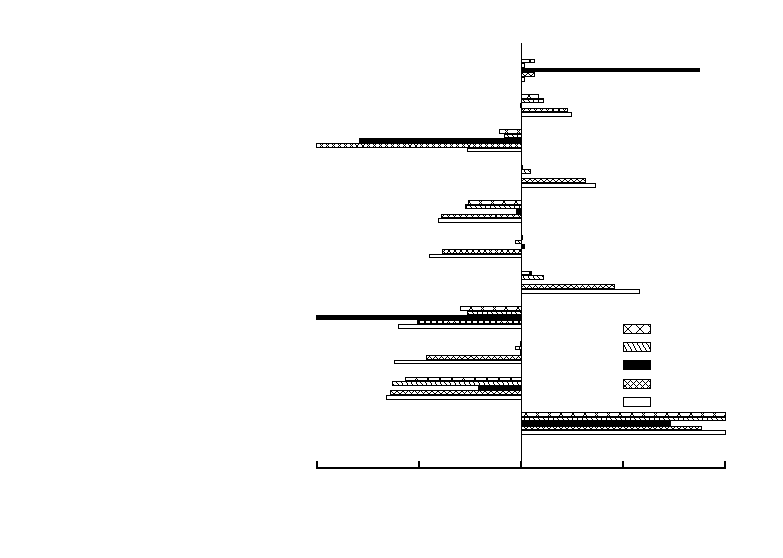
\includegraphics{CEMA_800}}%
    \gplfronttext
  \end{picture}%
\endgroup

  % GNUPLOT: LaTeX picture with Postscript
\begingroup
  \makeatletter
  \providecommand\color[2][]{%
    \GenericError{(gnuplot) \space\space\space\@spaces}{%
      Package color not loaded in conjunction with
      terminal option `colourtext'%
    }{See the gnuplot documentation for explanation.%
    }{Either use 'blacktext' in gnuplot or load the package
      color.sty in LaTeX.}%
    \renewcommand\color[2][]{}%
  }%
  \providecommand\includegraphics[2][]{%
    \GenericError{(gnuplot) \space\space\space\@spaces}{%
      Package graphicx or graphics not loaded%
    }{See the gnuplot documentation for explanation.%
    }{The gnuplot epslatex terminal needs graphicx.sty or graphics.sty.}%
    \renewcommand\includegraphics[2][]{}%
  }%
  \providecommand\rotatebox[2]{#2}%
  \@ifundefined{ifGPcolor}{%
    \newif\ifGPcolor
    \GPcolortrue
  }{}%
  \@ifundefined{ifGPblacktext}{%
    \newif\ifGPblacktext
    \GPblacktexttrue
  }{}%
  % define a \g@addto@macro without @ in the name:
  \let\gplgaddtomacro\g@addto@macro
  % define empty templates for all commands taking text:
  \gdef\gplbacktext{}%
  \gdef\gplfronttext{}%
  \makeatother
  \ifGPblacktext
    % no textcolor at all
    \def\colorrgb#1{}%
    \def\colorgray#1{}%
  \else
    % gray or color?
    \ifGPcolor
      \def\colorrgb#1{\color[rgb]{#1}}%
      \def\colorgray#1{\color[gray]{#1}}%
      \expandafter\def\csname LTw\endcsname{\color{white}}%
      \expandafter\def\csname LTb\endcsname{\color{black}}%
      \expandafter\def\csname LTa\endcsname{\color{black}}%
      \expandafter\def\csname LT0\endcsname{\color[rgb]{1,0,0}}%
      \expandafter\def\csname LT1\endcsname{\color[rgb]{0,1,0}}%
      \expandafter\def\csname LT2\endcsname{\color[rgb]{0,0,1}}%
      \expandafter\def\csname LT3\endcsname{\color[rgb]{1,0,1}}%
      \expandafter\def\csname LT4\endcsname{\color[rgb]{0,1,1}}%
      \expandafter\def\csname LT5\endcsname{\color[rgb]{1,1,0}}%
      \expandafter\def\csname LT6\endcsname{\color[rgb]{0,0,0}}%
      \expandafter\def\csname LT7\endcsname{\color[rgb]{1,0.3,0}}%
      \expandafter\def\csname LT8\endcsname{\color[rgb]{0.5,0.5,0.5}}%
    \else
      % gray
      \def\colorrgb#1{\color{black}}%
      \def\colorgray#1{\color[gray]{#1}}%
      \expandafter\def\csname LTw\endcsname{\color{white}}%
      \expandafter\def\csname LTb\endcsname{\color{black}}%
      \expandafter\def\csname LTa\endcsname{\color{black}}%
      \expandafter\def\csname LT0\endcsname{\color{black}}%
      \expandafter\def\csname LT1\endcsname{\color{black}}%
      \expandafter\def\csname LT2\endcsname{\color{black}}%
      \expandafter\def\csname LT3\endcsname{\color{black}}%
      \expandafter\def\csname LT4\endcsname{\color{black}}%
      \expandafter\def\csname LT5\endcsname{\color{black}}%
      \expandafter\def\csname LT6\endcsname{\color{black}}%
      \expandafter\def\csname LT7\endcsname{\color{black}}%
      \expandafter\def\csname LT8\endcsname{\color{black}}%
    \fi
  \fi
  \setlength{\unitlength}{0.0500bp}%
  \begin{picture}(7200.00,5040.00)%
    \gplgaddtomacro\gplbacktext{%
      \csname LTb\endcsname%
      \put(2748,1043){\makebox(0,0)[r]{\strut{}CH$_3$OCH$_2$$\Longleftrightarrow$CH$_2$O+CH$_3$}}%
      \put(2748,1383){\makebox(0,0)[r]{\strut{}CH$_3$OCH$_2$O$_2$$\Longleftrightarrow$CH$_2$OCH$_2$O$_2$H}}%
      \put(2748,1722){\makebox(0,0)[r]{\strut{}CH$_3$OCH$_3$+CH$_3$$\Longleftrightarrow$CH$_3$OCH$_2$+CH$_4$}}%
      \put(2748,2061){\makebox(0,0)[r]{\strut{}CH$_3$OCH$_3$+HO$_2$$\Longleftrightarrow$CH$_3$OCH$_2$+H$_2$O$_2$}}%
      \put(2748,2400){\makebox(0,0)[r]{\strut{}CH$_3$+CH$_3$+M$\Longleftrightarrow$C$_2$H$_6$+M}}%
      \put(2748,2740){\makebox(0,0)[r]{\strut{}CH$_3$+HO$_2$$\Longleftrightarrow$CH$_3$O+OH}}%
      \put(2748,3079){\makebox(0,0)[r]{\strut{}CH$_3$+HO$_2$$\Longleftrightarrow$CH$_4$+O$_2$}}%
      \put(2748,3418){\makebox(0,0)[r]{\strut{}CH$_2$OCH$_2$O$_2$H$\Longleftrightarrow$OH+CH$_2$O+CH$_2$O}}%
      \put(2748,3757){\makebox(0,0)[r]{\strut{}H$_2$O$_2$+M$\Longleftrightarrow$OH+OH+M}}%
      \put(2748,4097){\makebox(0,0)[r]{\strut{}H+O$_2$+M$\Longleftrightarrow$HO$_2$+M}}%
      \put(2748,4436){\makebox(0,0)[r]{\strut{}H+O$_2$$\Longleftrightarrow$O+OH}}%
      \put(2880,484){\makebox(0,0){\strut{}-1}}%
      \put(3861,484){\makebox(0,0){\strut{}-0.5}}%
      \put(4842,484){\makebox(0,0){\strut{} 0}}%
      \put(5822,484){\makebox(0,0){\strut{} 0.5}}%
      \put(6803,484){\makebox(0,0){\strut{} 1}}%
      \csname LTb\endcsname%
      \put(4841,154){\makebox(0,0){\strut{}Normalized Participation Index}}%
      \put(3076,1349){\makebox(0,0)[l]{\strut{}Point A}}%
      \put(3076,1518){\makebox(0,0)[l]{\strut{}Point B}}%
      \put(3076,1688){\makebox(0,0)[l]{\strut{}Point C}}%
      \put(3076,1857){\makebox(0,0)[l]{\strut{}Point D}}%
      \put(3076,2027){\makebox(0,0)[l]{\strut{}Point E}}%
      \put(3076,2231){\makebox(0,0)[l]{\strut{}$1100$ K}}%
    }%
    \gplgaddtomacro\gplfronttext{%
      \csname LTb\endcsname%
      \put(3532,1337){\makebox(0,0)[r]{\strut{} }}%
      \csname LTb\endcsname%
      \put(3532,1513){\makebox(0,0)[r]{\strut{} }}%
      \csname LTb\endcsname%
      \put(3532,1689){\makebox(0,0)[r]{\strut{} }}%
      \csname LTb\endcsname%
      \put(3532,1865){\makebox(0,0)[r]{\strut{} }}%
      \csname LTb\endcsname%
      \put(3532,2041){\makebox(0,0)[r]{\strut{} }}%
    }%
    \gplbacktext
    \put(0,0){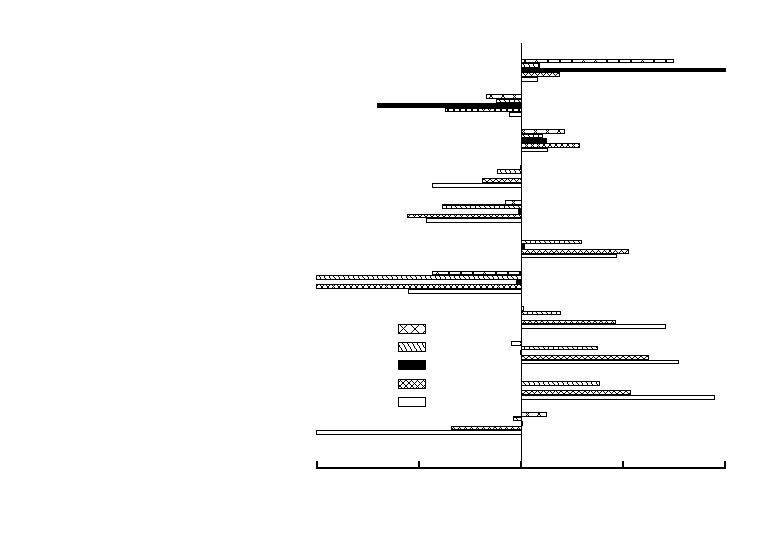
\includegraphics{CEMA_1100}}%
    \gplfronttext
  \end{picture}%
\endgroup

  \normalsize
  \caption{Normalized participation index at $800$ K and $1100$ K.  Sampled locations are indicated in Fig.~\ref{fig:dynamics-HRR_T}.}
  \label{fig:CEMA_T}
\end{figure}

The results are summarized in Fig.~\ref{fig:CEMA_T}, where three representative locations along the $Z_{\rm st}$ iso-contour approaching the flame front and two locations ahead of and at the reaction front at $Z = 0.2$ were sampled.  For the three lower coflow temperature cases, similar chemical patterns were found.  Upstream of the flame front, the chemical explosive mode is positive, indicating that the mixtures have the potential to explode; downstream of the flame front, the chemical explosive mode becomes negative, meaning that the mixtures are composed of burned products.  Following the $Z_{\rm st}$ iso-contour, the hydrogen peroxide chain branching reaction (H$_2$O$_2$ + M $\Longleftrightarrow$ OH + OH + M) is the reaction that has the largest contribution to the explosive mode, showing the dominant role of autoignition chain branching~\cite{westbrook00}.  The characteristic DME low-temperature chemistry is also important upstream of the flame, where methoxymethylperoxy radical formation (CH$_3$OCH$_2$ + O$_2$ $\Longleftrightarrow$ CH$_3$OCH$_2$O$_2$) and isomerization (CH$_3$OCH$_2$O$_2$ $\Longleftrightarrow$ CH$_2$OCH$_2$O$_2$H) promote the explosion, while the $\beta$-scission reaction (CH$_2$OCH$_2$O$_2$H $\Longleftrightarrow$ OH + CH$_2$O + CH$_2$O) retards the explosion.  Approaching the flame front, the H radical recombination reaction (H + O$_2$ + M $\Longleftrightarrow$ HO$_2$ + M) becomes important for the $700-900$ K cases, due to the fact that the H radicals generated at the reaction zone diffuse upstream and undergo three-body recombination reactions under the high pressure, low temperature condition.  Further downstream where the heat release rate peaks, the hydrogen branching reaction (H + O$_2$ $\Longleftrightarrow$ O + OH) becomes the most important chain branching reaction as it is activated at high temperatures~\cite{westbrook00}.

CEMA conducted along the $Z = 0.2$ iso-contour, which crosses the rich heat release front in the $800$ and $900$ K cases, shows different chemical mode evolution.  The H$_2$O$_2$ chain branching reaction is always the dominant reaction that promotes the explosive mode, while the H radical recombination reaction and the H branching reaction are less important ahead of the rich heat release front and at the front.  

On the contrary, although low-temperature chemistry is still important for the $1100$ K case upstream of the reaction zone and the hydrogen chain branching reaction promotes explosion in the reaction zone, the hydrogen peroxide chain branching reaction is not very important for all the sampled locations.  Since the hydrogen peroxide reaction is the crucial chain branching reaction for the autoignition process, it is concluded that the $1100$ K case is less affected by autoignition chemistry than the lower boundary temperature cases.  

\subsubsection{Lagrangian Flamelet Analysis} \label{sec:LFA}

The above species profile analysis and CEMA results have demonstrated that autoignition chemistry is crucial to the complex flame structure in the $700$ to $900$ K cases.  However, the role that autoignition plays in the stabilization still needs further investigation.  To elucidate the role of autoignition for the current flow configuration, a direct comparison with the homogeneous counterpart for a Lagrangian flow particle is insufficient, for no transport process is considered in homogeneous autoignition.  In the current two-dimensional configuration, however, transport processes are present in two directions: parallel and normal to the mixture fraction gradient.  These transport processes might be important: first, the temperature and species stratification parallel to the mixture fraction gradient can significantly modify the ignition characteristics, especially for fuels with NTC chemistry, as shown in Chapter~\ref{ch:NTC}.  Second, flame propagation normal to the mixture fraction gradient can also influence the autoignition front through thermal and radical back diffusion.

To demonstrate the dominant transport direction as well as the stabilization mechanism, one-dimensional unsteady flamelet analysis was conducted to account for unsteadiness (convection), chemical reactions, and diffusion parallel to the mixture fraction gradient, while neglecting the transport process in the normal direction.  As a consequence, the unsteady flamelet is able to capture inhomogeneous autoignition, with diffusion allowed only in one direction.  Following the mixture fraction iso-contour, the spatial information from the two-dimensional computation could be interpreted as the time history of the corresponding mixture in the Lagrangian frame.  If the one-dimensional unsteady flamelet predicts this time history, only the transport processes parallel to the mixture fraction gradient are important, and, therefore, the thermal structure is stabilized by inhomogeneous autoignition.  Conversely, if the unsteady flamelet solutions do not agree with the two-dimensional computations, the transport processes along the mixture fraction iso-contour are not negligible compared to the gradient direction.  Therefore, premixed flame propagation is the dominant stabilization mechanism, or, at least, stabilization is strongly affected by flame back diffusion.

The unsteady flamelet model developed by Pitsch \emph{et al.}~\cite{pitsch98a}, referred to as Lagrangian Flamelet Analysis (LFA), was adopted.  Due to the mixing processes, the scalar dissipation rate $\chi$, which can influence the flamelet solution significantly, decreases in the streamwise direction.  Therefore, this dissipation rate variation must be considered when computing a flamelet as it evolves downstream.

The unsteady flamelet was computed with FlameMaster~\cite{flamemaster}, and the dissipation rate was specified as a function of the flamelet time.  The flamelet time was computed from the two-dimensional computational results, along the stoichiometric mixture fraction $Z_{\rm st}$ iso-contour: 
 \begin{equation} \label{eq:t}
t = \int ^{x}_{0} \frac{1}{(u + u_Z)(x')|(Z=Z_{\rm st})} dx'.
\end{equation}
This formulation is otherwise the same as that of Pitsch \emph {et al.}~\cite{pitsch98a}, except that, in addition to the axial component of fluid convection velocity $u$, the axial component of the mixture fraction iso-contour propagation speed relative to the fluid convection $u_Z$ is also taken into account.  The expression for the constant property scalar iso-surface velocity relative to the local fluid motion was derived by Pope~\cite{pope88}, and the current work adopts the formulation derived by Lignell \emph {et al.}~\cite{lignell07} for variable properties:
\begin{equation}
\mathbf{u_Z} = -\frac{\nabla \cdot (\rho D_Z \nabla Z) }{\rho |\nabla Z|} \mathbf{n},
\end{equation}  
where $D_Z$ is the mixture fraction diffusivity, which is defined in Sec.~\ref{sec:dynamics-computation}, and $\rho$ the density.  The normal vector \textbf{n}, defined as
\begin{equation}
\mathbf{n} = \frac{\nabla Z}{|\nabla Z|},
\end{equation}
indicates the direction of this diffusion induced relative velocity.
The dissipation rate along the $Z_{\rm st} = 0.1005$ iso-contour obtained from the two-dimensional computation was then correlated with this flamelet time and provided as the input for the LFA calculation.  The dissipation rates at other mixture fractions were computed assuming the following form~\cite{petersbook}:
\begin{equation} \label{eq:Zref}
\chi{(Z)} = \chi{(Z_{\rm st})} \frac{\exp{(-2[{\rm erfc}^{-1}(2Z)]^2)}}{\exp{(-2[{\rm erfc}^{-1}(2Z_{\rm st})]^2)}} = \chi{(Z_{\rm st})} f(Z;Z_{\rm st}).
\end{equation}

To validate this formulation in the current configuration, the dissipation rates along different mixture fraction iso-contours were sampled from the two-dimensional computations, normalized using Eq.~\ref{eq:Zref}, and compared with the sampling along the $Z_{\rm st}$ iso-contour.  As shown in Fig.~\ref{fig:Zref}, the normalized dissipation rates at different mixture fractions all collapse to the value at $Z_{\rm st}$.  Therefore, only the dissipation rate samplings along the $Z_{\rm st}$ iso-contour were needed to perform the unsteady flamelet calculation.

\begin{figure}
  \centering
  \scriptsize
  % GNUPLOT: LaTeX picture with Postscript
\begingroup
  \makeatletter
  \providecommand\color[2][]{%
    \GenericError{(gnuplot) \space\space\space\@spaces}{%
      Package color not loaded in conjunction with
      terminal option `colourtext'%
    }{See the gnuplot documentation for explanation.%
    }{Either use 'blacktext' in gnuplot or load the package
      color.sty in LaTeX.}%
    \renewcommand\color[2][]{}%
  }%
  \providecommand\includegraphics[2][]{%
    \GenericError{(gnuplot) \space\space\space\@spaces}{%
      Package graphicx or graphics not loaded%
    }{See the gnuplot documentation for explanation.%
    }{The gnuplot epslatex terminal needs graphicx.sty or graphics.sty.}%
    \renewcommand\includegraphics[2][]{}%
  }%
  \providecommand\rotatebox[2]{#2}%
  \@ifundefined{ifGPcolor}{%
    \newif\ifGPcolor
    \GPcolortrue
  }{}%
  \@ifundefined{ifGPblacktext}{%
    \newif\ifGPblacktext
    \GPblacktexttrue
  }{}%
  % define a \g@addto@macro without @ in the name:
  \let\gplgaddtomacro\g@addto@macro
  % define empty templates for all commands taking text:
  \gdef\gplbacktext{}%
  \gdef\gplfronttext{}%
  \makeatother
  \ifGPblacktext
    % no textcolor at all
    \def\colorrgb#1{}%
    \def\colorgray#1{}%
  \else
    % gray or color?
    \ifGPcolor
      \def\colorrgb#1{\color[rgb]{#1}}%
      \def\colorgray#1{\color[gray]{#1}}%
      \expandafter\def\csname LTw\endcsname{\color{white}}%
      \expandafter\def\csname LTb\endcsname{\color{black}}%
      \expandafter\def\csname LTa\endcsname{\color{black}}%
      \expandafter\def\csname LT0\endcsname{\color[rgb]{1,0,0}}%
      \expandafter\def\csname LT1\endcsname{\color[rgb]{0,1,0}}%
      \expandafter\def\csname LT2\endcsname{\color[rgb]{0,0,1}}%
      \expandafter\def\csname LT3\endcsname{\color[rgb]{1,0,1}}%
      \expandafter\def\csname LT4\endcsname{\color[rgb]{0,1,1}}%
      \expandafter\def\csname LT5\endcsname{\color[rgb]{1,1,0}}%
      \expandafter\def\csname LT6\endcsname{\color[rgb]{0,0,0}}%
      \expandafter\def\csname LT7\endcsname{\color[rgb]{1,0.3,0}}%
      \expandafter\def\csname LT8\endcsname{\color[rgb]{0.5,0.5,0.5}}%
    \else
      % gray
      \def\colorrgb#1{\color{black}}%
      \def\colorgray#1{\color[gray]{#1}}%
      \expandafter\def\csname LTw\endcsname{\color{white}}%
      \expandafter\def\csname LTb\endcsname{\color{black}}%
      \expandafter\def\csname LTa\endcsname{\color{black}}%
      \expandafter\def\csname LT0\endcsname{\color{black}}%
      \expandafter\def\csname LT1\endcsname{\color{black}}%
      \expandafter\def\csname LT2\endcsname{\color{black}}%
      \expandafter\def\csname LT3\endcsname{\color{black}}%
      \expandafter\def\csname LT4\endcsname{\color{black}}%
      \expandafter\def\csname LT5\endcsname{\color{black}}%
      \expandafter\def\csname LT6\endcsname{\color{black}}%
      \expandafter\def\csname LT7\endcsname{\color{black}}%
      \expandafter\def\csname LT8\endcsname{\color{black}}%
    \fi
  \fi
  \setlength{\unitlength}{0.0500bp}%
  \begin{picture}(7200.00,5040.00)%
    \gplgaddtomacro\gplbacktext{%
      \csname LTb\endcsname%
      \put(946,704){\makebox(0,0)[r]{\strut{} 0}}%
      \put(946,1383){\makebox(0,0)[r]{\strut{} 50}}%
      \put(946,2061){\makebox(0,0)[r]{\strut{} 100}}%
      \put(946,2740){\makebox(0,0)[r]{\strut{} 150}}%
      \put(946,3418){\makebox(0,0)[r]{\strut{} 200}}%
      \put(946,4097){\makebox(0,0)[r]{\strut{} 250}}%
      \put(946,4775){\makebox(0,0)[r]{\strut{} 300}}%
      \put(1078,484){\makebox(0,0){\strut{} 0}}%
      \put(1841,484){\makebox(0,0){\strut{} 0.2}}%
      \put(2605,484){\makebox(0,0){\strut{} 0.4}}%
      \put(3368,484){\makebox(0,0){\strut{} 0.6}}%
      \put(4131,484){\makebox(0,0){\strut{} 0.8}}%
      \put(4895,484){\makebox(0,0){\strut{} 1}}%
      \put(5658,484){\makebox(0,0){\strut{} 1.2}}%
      \put(6421,484){\makebox(0,0){\strut{} 1.4}}%
      \put(176,2739){\rotatebox{-270}{\makebox(0,0){\strut{}\vspace{-28pt}$\frac{\chi(Z)}{f(Z,Z_{\rm st})}$ [1/s]}}}%
      \put(3940,154){\makebox(0,0){\strut{}Time [ms]}}%
    }%
    \gplgaddtomacro\gplfronttext{%
      \csname LTb\endcsname%
      \put(5816,4602){\makebox(0,0)[r]{\strut{}$Z = Z_{\rm st}$}}%
      \csname LTb\endcsname%
      \put(5816,4382){\makebox(0,0)[r]{\strut{}$Z = 0.2$}}%
      \csname LTb\endcsname%
      \put(5816,4162){\makebox(0,0)[r]{\strut{}$Z = 0.4$}}%
      \csname LTb\endcsname%
      \put(5816,3942){\makebox(0,0)[r]{\strut{}$Z = 0.6$}}%
    }%
    \gplbacktext
    \put(0,0){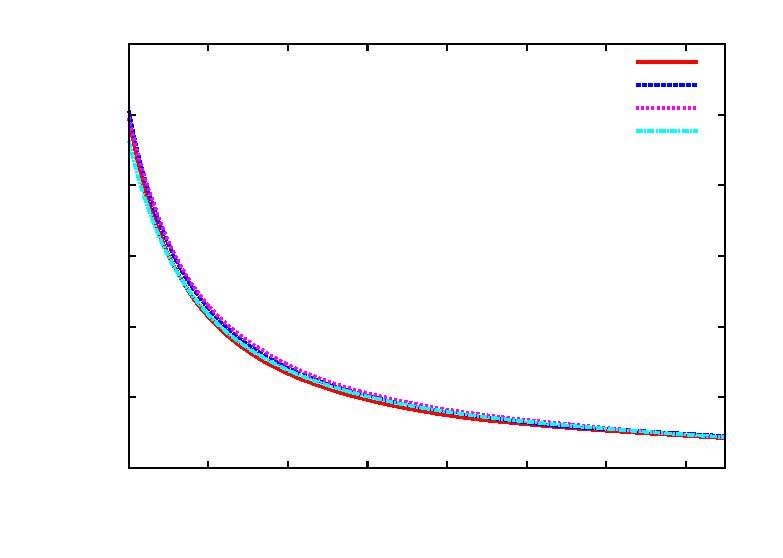
\includegraphics{Zref}}%
    \gplfronttext
  \end{picture}%
\endgroup

  \normalsize
  \caption{$\frac{\chi(Z)}{f(Z;Z_{\rm st})}$, using Eq.~\ref{eq:Zref}, from the two-dimensional calculations at $800$ K.}
  \label{fig:Zref}
\end{figure}

To account for the differential diffusion, species Lewis numbers for LFA  were specified the same as in the two-dimensional computations.  The governing equations for species and temperature follow Eq. $24$ and $25$ in Pitsch and Peters~\cite{pitsch98b}.

The time history of the dissipation rate $\chi_{\rm st}$ was specified in LFA according to the two-dimensional computation.  To avoid the ill-defined Lagrangian time in the recirculation zone, time zero was defined at a downstream location ten times the thickness of the wall.  Accordingly, the species and temperature profiles along the radial cut at this location were specified as the initial conditions for the flamelet.  Based on these initial conditions and $\chi_{\rm st}$ time history profiles, the unsteady flamelets were calculated and compared with the two-dimensional computational results for $Z_{\rm st}$, $Z = 0.2$, and $Z = 0.3$.

\begin{figure}
  \centering
  \scriptsize
  \resizebox{1.15\textwidth}{!}{% GNUPLOT: LaTeX picture with Postscript
\begingroup
  \makeatletter
  \providecommand\color[2][]{%
    \GenericError{(gnuplot) \space\space\space\@spaces}{%
      Package color not loaded in conjunction with
      terminal option `colourtext'%
    }{See the gnuplot documentation for explanation.%
    }{Either use 'blacktext' in gnuplot or load the package
      color.sty in LaTeX.}%
    \renewcommand\color[2][]{}%
  }%
  \providecommand\includegraphics[2][]{%
    \GenericError{(gnuplot) \space\space\space\@spaces}{%
      Package graphicx or graphics not loaded%
    }{See the gnuplot documentation for explanation.%
    }{The gnuplot epslatex terminal needs graphicx.sty or graphics.sty.}%
    \renewcommand\includegraphics[2][]{}%
  }%
  \providecommand\rotatebox[2]{#2}%
  \@ifundefined{ifGPcolor}{%
    \newif\ifGPcolor
    \GPcolortrue
  }{}%
  \@ifundefined{ifGPblacktext}{%
    \newif\ifGPblacktext
    \GPblacktexttrue
  }{}%
  % define a \g@addto@macro without @ in the name:
  \let\gplgaddtomacro\g@addto@macro
  % define empty templates for all commands taking text:
  \gdef\gplbacktext{}%
  \gdef\gplfronttext{}%
  \makeatother
  \ifGPblacktext
    % no textcolor at all
    \def\colorrgb#1{}%
    \def\colorgray#1{}%
  \else
    % gray or color?
    \ifGPcolor
      \def\colorrgb#1{\color[rgb]{#1}}%
      \def\colorgray#1{\color[gray]{#1}}%
      \expandafter\def\csname LTw\endcsname{\color{white}}%
      \expandafter\def\csname LTb\endcsname{\color{black}}%
      \expandafter\def\csname LTa\endcsname{\color{black}}%
      \expandafter\def\csname LT0\endcsname{\color[rgb]{1,0,0}}%
      \expandafter\def\csname LT1\endcsname{\color[rgb]{0,1,0}}%
      \expandafter\def\csname LT2\endcsname{\color[rgb]{0,0,1}}%
      \expandafter\def\csname LT3\endcsname{\color[rgb]{1,0,1}}%
      \expandafter\def\csname LT4\endcsname{\color[rgb]{0,1,1}}%
      \expandafter\def\csname LT5\endcsname{\color[rgb]{1,1,0}}%
      \expandafter\def\csname LT6\endcsname{\color[rgb]{0,0,0}}%
      \expandafter\def\csname LT7\endcsname{\color[rgb]{1,0.3,0}}%
      \expandafter\def\csname LT8\endcsname{\color[rgb]{0.5,0.5,0.5}}%
    \else
      % gray
      \def\colorrgb#1{\color{black}}%
      \def\colorgray#1{\color[gray]{#1}}%
      \expandafter\def\csname LTw\endcsname{\color{white}}%
      \expandafter\def\csname LTb\endcsname{\color{black}}%
      \expandafter\def\csname LTa\endcsname{\color{black}}%
      \expandafter\def\csname LT0\endcsname{\color{black}}%
      \expandafter\def\csname LT1\endcsname{\color{black}}%
      \expandafter\def\csname LT2\endcsname{\color{black}}%
      \expandafter\def\csname LT3\endcsname{\color{black}}%
      \expandafter\def\csname LT4\endcsname{\color{black}}%
      \expandafter\def\csname LT5\endcsname{\color{black}}%
      \expandafter\def\csname LT6\endcsname{\color{black}}%
      \expandafter\def\csname LT7\endcsname{\color{black}}%
      \expandafter\def\csname LT8\endcsname{\color{black}}%
    \fi
  \fi
  \setlength{\unitlength}{0.0500bp}%
  \begin{picture}(11520.00,6048.00)%
    \gplgaddtomacro\gplbacktext{%
      \csname LTb\endcsname%
      \put(7990,4756){\makebox(0,0)[r]{\strut{} 800}}%
      \put(7990,4961){\makebox(0,0)[r]{\strut{} 1200}}%
      \put(7990,5167){\makebox(0,0)[r]{\strut{} 1600}}%
      \put(7990,5372){\makebox(0,0)[r]{\strut{} 2000}}%
      \put(7990,5578){\makebox(0,0)[r]{\strut{} 2400}}%
      \put(7990,5783){\makebox(0,0)[r]{\strut{} 2800}}%
      \put(8122,4536){\makebox(0,0){\strut{} 0}}%
      \put(8440,4536){\makebox(0,0){\strut{} 0.25}}%
      \put(8759,4536){\makebox(0,0){\strut{} 0.5}}%
      \put(9077,4536){\makebox(0,0){\strut{} 0.75}}%
      \put(9395,4536){\makebox(0,0){\strut{} 1}}%
      \put(7088,5269){\rotatebox{-270}{\makebox(0,0){\strut{}\vspace{-48pt}$T$ [K]}}}%
      \put(8758,4206){\makebox(0,0){\strut{}\vspace{12pt}Time [ms]}}%
      \put(1728,6047){\makebox(0,0)[l]{\strut{}$700$ K}}%
      \put(4032,6047){\makebox(0,0)[l]{\strut{}$800$ K}}%
      \put(6335,6047){\makebox(0,0)[l]{\strut{}$900$ K}}%
      \put(8639,6047){\makebox(0,0)[l]{\strut{}$1100$ K}}%
      \put(-229,1209){\makebox(0,0)[l]{\strut{}$Z = 0.3$}}%
      \put(-229,3205){\makebox(0,0)[l]{\strut{}$Z = 0.2$}}%
      \put(-229,5261){\makebox(0,0)[l]{\strut{}$Z = Z_{\rm st}$}}%
    }%
    \gplgaddtomacro\gplfronttext{%
    }%
    \gplgaddtomacro\gplbacktext{%
      \csname LTb\endcsname%
      \put(7990,2941){\makebox(0,0)[r]{\strut{} 800}}%
      \put(7990,3147){\makebox(0,0)[r]{\strut{} 1200}}%
      \put(7990,3352){\makebox(0,0)[r]{\strut{} 1600}}%
      \put(7990,3558){\makebox(0,0)[r]{\strut{} 2000}}%
      \put(7990,3763){\makebox(0,0)[r]{\strut{} 2400}}%
      \put(7990,3969){\makebox(0,0)[r]{\strut{} 2800}}%
      \put(8122,2721){\makebox(0,0){\strut{} 0}}%
      \put(8440,2721){\makebox(0,0){\strut{} 0.25}}%
      \put(8759,2721){\makebox(0,0){\strut{} 0.5}}%
      \put(9077,2721){\makebox(0,0){\strut{} 0.75}}%
      \put(9395,2721){\makebox(0,0){\strut{} 1}}%
      \put(7088,3455){\rotatebox{-270}{\makebox(0,0){\strut{}\vspace{-48pt}$T$ [K]}}}%
      \put(8758,2391){\makebox(0,0){\strut{}\vspace{12pt}Time [ms]}}%
    }%
    \gplgaddtomacro\gplfronttext{%
    }%
    \gplgaddtomacro\gplbacktext{%
      \csname LTb\endcsname%
      \put(7990,1187){\makebox(0,0)[r]{\strut{} 400}}%
      \put(7990,1393){\makebox(0,0)[r]{\strut{} 800}}%
      \put(7990,1598){\makebox(0,0)[r]{\strut{} 1200}}%
      \put(7990,1804){\makebox(0,0)[r]{\strut{} 1600}}%
      \put(7990,2009){\makebox(0,0)[r]{\strut{} 2000}}%
      \put(7990,2215){\makebox(0,0)[r]{\strut{} 2400}}%
      \put(8122,967){\makebox(0,0){\strut{} 0}}%
      \put(8440,967){\makebox(0,0){\strut{} 0.25}}%
      \put(8759,967){\makebox(0,0){\strut{} 0.5}}%
      \put(9077,967){\makebox(0,0){\strut{} 0.75}}%
      \put(9395,967){\makebox(0,0){\strut{} 1}}%
      \put(7088,1701){\rotatebox{-270}{\makebox(0,0){\strut{}\vspace{-48pt}$T$ [K]}}}%
      \put(8758,637){\makebox(0,0){\strut{}\vspace{12pt}Time [ms]}}%
    }%
    \gplgaddtomacro\gplfronttext{%
    }%
    \gplgaddtomacro\gplbacktext{%
      \csname LTb\endcsname%
      \put(5686,4756){\makebox(0,0)[r]{\strut{} 600}}%
      \put(5686,4961){\makebox(0,0)[r]{\strut{} 1000}}%
      \put(5686,5167){\makebox(0,0)[r]{\strut{} 1400}}%
      \put(5686,5372){\makebox(0,0)[r]{\strut{} 1800}}%
      \put(5686,5578){\makebox(0,0)[r]{\strut{} 2200}}%
      \put(5686,5783){\makebox(0,0)[r]{\strut{} 2600}}%
      \put(5818,4536){\makebox(0,0){\strut{} 0}}%
      \put(6136,4536){\makebox(0,0){\strut{} 0.3}}%
      \put(6455,4536){\makebox(0,0){\strut{} 0.6}}%
      \put(6773,4536){\makebox(0,0){\strut{} 0.9}}%
      \put(7091,4536){\makebox(0,0){\strut{} 1.2}}%
      \put(4784,5269){\rotatebox{-270}{\makebox(0,0){\strut{}\vspace{-48pt}$T$ [K]}}}%
      \put(6454,4206){\makebox(0,0){\strut{}\vspace{12pt}Time [ms]}}%
    }%
    \gplgaddtomacro\gplfronttext{%
    }%
    \gplgaddtomacro\gplbacktext{%
      \csname LTb\endcsname%
      \put(5686,2941){\makebox(0,0)[r]{\strut{} 600}}%
      \put(5686,3147){\makebox(0,0)[r]{\strut{} 1000}}%
      \put(5686,3352){\makebox(0,0)[r]{\strut{} 1400}}%
      \put(5686,3558){\makebox(0,0)[r]{\strut{} 1800}}%
      \put(5686,3763){\makebox(0,0)[r]{\strut{} 2200}}%
      \put(5686,3969){\makebox(0,0)[r]{\strut{} 2600}}%
      \put(5818,2721){\makebox(0,0){\strut{} 0}}%
      \put(6136,2721){\makebox(0,0){\strut{} 0.3}}%
      \put(6455,2721){\makebox(0,0){\strut{} 0.6}}%
      \put(6773,2721){\makebox(0,0){\strut{} 0.9}}%
      \put(7091,2721){\makebox(0,0){\strut{} 1.2}}%
      \put(4784,3455){\rotatebox{-270}{\makebox(0,0){\strut{}\vspace{-48pt}$T$ [K]}}}%
      \put(6454,2391){\makebox(0,0){\strut{}\vspace{12pt}Time [ms]}}%
    }%
    \gplgaddtomacro\gplfronttext{%
    }%
    \gplgaddtomacro\gplbacktext{%
      \csname LTb\endcsname%
      \put(5686,1187){\makebox(0,0)[r]{\strut{} 400}}%
      \put(5686,1393){\makebox(0,0)[r]{\strut{} 800}}%
      \put(5686,1598){\makebox(0,0)[r]{\strut{} 1200}}%
      \put(5686,1804){\makebox(0,0)[r]{\strut{} 1600}}%
      \put(5686,2009){\makebox(0,0)[r]{\strut{} 2000}}%
      \put(5686,2215){\makebox(0,0)[r]{\strut{} 2400}}%
      \put(5818,967){\makebox(0,0){\strut{} 0}}%
      \put(6136,967){\makebox(0,0){\strut{} 0.3}}%
      \put(6455,967){\makebox(0,0){\strut{} 0.6}}%
      \put(6773,967){\makebox(0,0){\strut{} 0.9}}%
      \put(7091,967){\makebox(0,0){\strut{} 1.2}}%
      \put(4784,1701){\rotatebox{-270}{\makebox(0,0){\strut{}\vspace{-48pt}$T$ [K]}}}%
      \put(6454,637){\makebox(0,0){\strut{}\vspace{12pt}Time [ms]}}%
    }%
    \gplgaddtomacro\gplfronttext{%
    }%
    \gplgaddtomacro\gplbacktext{%
      \csname LTb\endcsname%
      \put(3382,4756){\makebox(0,0)[r]{\strut{} 600}}%
      \put(3382,4961){\makebox(0,0)[r]{\strut{} 1000}}%
      \put(3382,5167){\makebox(0,0)[r]{\strut{} 1400}}%
      \put(3382,5372){\makebox(0,0)[r]{\strut{} 1800}}%
      \put(3382,5578){\makebox(0,0)[r]{\strut{} 2200}}%
      \put(3382,5783){\makebox(0,0)[r]{\strut{} 2600}}%
      \put(3514,4536){\makebox(0,0){\strut{} 0}}%
      \put(3832,4536){\makebox(0,0){\strut{} 0.6}}%
      \put(4151,4536){\makebox(0,0){\strut{} 1.2}}%
      \put(4469,4536){\makebox(0,0){\strut{} 1.8}}%
      \put(4787,4536){\makebox(0,0){\strut{} 2.4}}%
      \put(2480,5269){\rotatebox{-270}{\makebox(0,0){\strut{}\vspace{-48pt}$T$ [K]}}}%
      \put(4150,4206){\makebox(0,0){\strut{}\vspace{12pt}Time [ms]}}%
    }%
    \gplgaddtomacro\gplfronttext{%
    }%
    \gplgaddtomacro\gplbacktext{%
      \csname LTb\endcsname%
      \put(3382,2941){\makebox(0,0)[r]{\strut{} 600}}%
      \put(3382,3147){\makebox(0,0)[r]{\strut{} 1000}}%
      \put(3382,3352){\makebox(0,0)[r]{\strut{} 1400}}%
      \put(3382,3558){\makebox(0,0)[r]{\strut{} 1800}}%
      \put(3382,3763){\makebox(0,0)[r]{\strut{} 2200}}%
      \put(3382,3969){\makebox(0,0)[r]{\strut{} 2600}}%
      \put(3514,2721){\makebox(0,0){\strut{} 0}}%
      \put(3832,2721){\makebox(0,0){\strut{} 0.6}}%
      \put(4151,2721){\makebox(0,0){\strut{} 1.2}}%
      \put(4469,2721){\makebox(0,0){\strut{} 1.8}}%
      \put(4787,2721){\makebox(0,0){\strut{} 2.4}}%
      \put(2480,3455){\rotatebox{-270}{\makebox(0,0){\strut{}\vspace{-48pt}$T$ [K]}}}%
      \put(4150,2391){\makebox(0,0){\strut{}\vspace{12pt}Time [ms]}}%
    }%
    \gplgaddtomacro\gplfronttext{%
    }%
    \gplgaddtomacro\gplbacktext{%
      \csname LTb\endcsname%
      \put(3382,1187){\makebox(0,0)[r]{\strut{} 400}}%
      \put(3382,1393){\makebox(0,0)[r]{\strut{} 800}}%
      \put(3382,1598){\makebox(0,0)[r]{\strut{} 1200}}%
      \put(3382,1804){\makebox(0,0)[r]{\strut{} 1600}}%
      \put(3382,2009){\makebox(0,0)[r]{\strut{} 2000}}%
      \put(3382,2215){\makebox(0,0)[r]{\strut{} 2400}}%
      \put(3514,967){\makebox(0,0){\strut{} 0}}%
      \put(3832,967){\makebox(0,0){\strut{} 0.6}}%
      \put(4151,967){\makebox(0,0){\strut{} 1.2}}%
      \put(4469,967){\makebox(0,0){\strut{} 1.8}}%
      \put(4787,967){\makebox(0,0){\strut{} 2.4}}%
      \put(2480,1701){\rotatebox{-270}{\makebox(0,0){\strut{}\vspace{-48pt}$T$ [K]}}}%
      \put(4150,637){\makebox(0,0){\strut{}\vspace{12pt}Time [ms]}}%
    }%
    \gplgaddtomacro\gplfronttext{%
    }%
    \gplgaddtomacro\gplbacktext{%
      \csname LTb\endcsname%
      \put(1078,4756){\makebox(0,0)[r]{\strut{} 400}}%
      \put(1078,4961){\makebox(0,0)[r]{\strut{} 800}}%
      \put(1078,5167){\makebox(0,0)[r]{\strut{} 1200}}%
      \put(1078,5372){\makebox(0,0)[r]{\strut{} 1600}}%
      \put(1078,5578){\makebox(0,0)[r]{\strut{} 2000}}%
      \put(1078,5783){\makebox(0,0)[r]{\strut{} 2400}}%
      \put(1210,4536){\makebox(0,0){\strut{} 0}}%
      \put(1528,4536){\makebox(0,0){\strut{} 2.5}}%
      \put(1847,4536){\makebox(0,0){\strut{} 5}}%
      \put(2165,4536){\makebox(0,0){\strut{} 7.5}}%
      \put(2483,4536){\makebox(0,0){\strut{} 10}}%
      \put(176,5269){\rotatebox{-270}{\makebox(0,0){\strut{}\vspace{-48pt}$T$ [K]}}}%
      \put(1846,4206){\makebox(0,0){\strut{}\vspace{12pt}Time [ms]}}%
    }%
    \gplgaddtomacro\gplfronttext{%
    }%
    \gplgaddtomacro\gplbacktext{%
      \csname LTb\endcsname%
      \put(1078,2941){\makebox(0,0)[r]{\strut{} 400}}%
      \put(1078,3147){\makebox(0,0)[r]{\strut{} 800}}%
      \put(1078,3352){\makebox(0,0)[r]{\strut{} 1200}}%
      \put(1078,3558){\makebox(0,0)[r]{\strut{} 1600}}%
      \put(1078,3763){\makebox(0,0)[r]{\strut{} 2000}}%
      \put(1078,3969){\makebox(0,0)[r]{\strut{} 2400}}%
      \put(1210,2721){\makebox(0,0){\strut{} 0}}%
      \put(1528,2721){\makebox(0,0){\strut{} 2.5}}%
      \put(1847,2721){\makebox(0,0){\strut{} 5}}%
      \put(2165,2721){\makebox(0,0){\strut{} 7.5}}%
      \put(2483,2721){\makebox(0,0){\strut{} 10}}%
      \put(176,3455){\rotatebox{-270}{\makebox(0,0){\strut{}\vspace{-48pt}$T$ [K]}}}%
      \put(1846,2391){\makebox(0,0){\strut{}\vspace{12pt}Time [ms]}}%
    }%
    \gplgaddtomacro\gplfronttext{%
    }%
    \gplgaddtomacro\gplbacktext{%
      \csname LTb\endcsname%
      \put(1078,1187){\makebox(0,0)[r]{\strut{} 200}}%
      \put(1078,1393){\makebox(0,0)[r]{\strut{} 600}}%
      \put(1078,1598){\makebox(0,0)[r]{\strut{} 1000}}%
      \put(1078,1804){\makebox(0,0)[r]{\strut{} 1400}}%
      \put(1078,2009){\makebox(0,0)[r]{\strut{} 1800}}%
      \put(1078,2215){\makebox(0,0)[r]{\strut{} 2200}}%
      \put(1210,967){\makebox(0,0){\strut{} 0}}%
      \put(1528,967){\makebox(0,0){\strut{} 2.5}}%
      \put(1847,967){\makebox(0,0){\strut{} 5}}%
      \put(2165,967){\makebox(0,0){\strut{} 7.5}}%
      \put(2483,967){\makebox(0,0){\strut{} 10}}%
      \put(176,1701){\rotatebox{-270}{\makebox(0,0){\strut{}\vspace{-48pt}$T$ [K]}}}%
      \put(1846,637){\makebox(0,0){\strut{}\vspace{12pt}Time [ms]}}%
      \put(4608,242){\makebox(0,0)[l]{\strut{}2D-CFD}}%
      \put(5760,242){\makebox(0,0)[l]{\strut{}1D-LFA}}%
    }%
    \gplgaddtomacro\gplfronttext{%
      \csname LTb\endcsname%
      \put(4050,253){\makebox(0,0)[r]{\strut{} }}%
      \csname LTb\endcsname%
      \put(5169,253){\makebox(0,0)[r]{\strut{}    }}%
    }%
    \gplbacktext
    \put(0,0){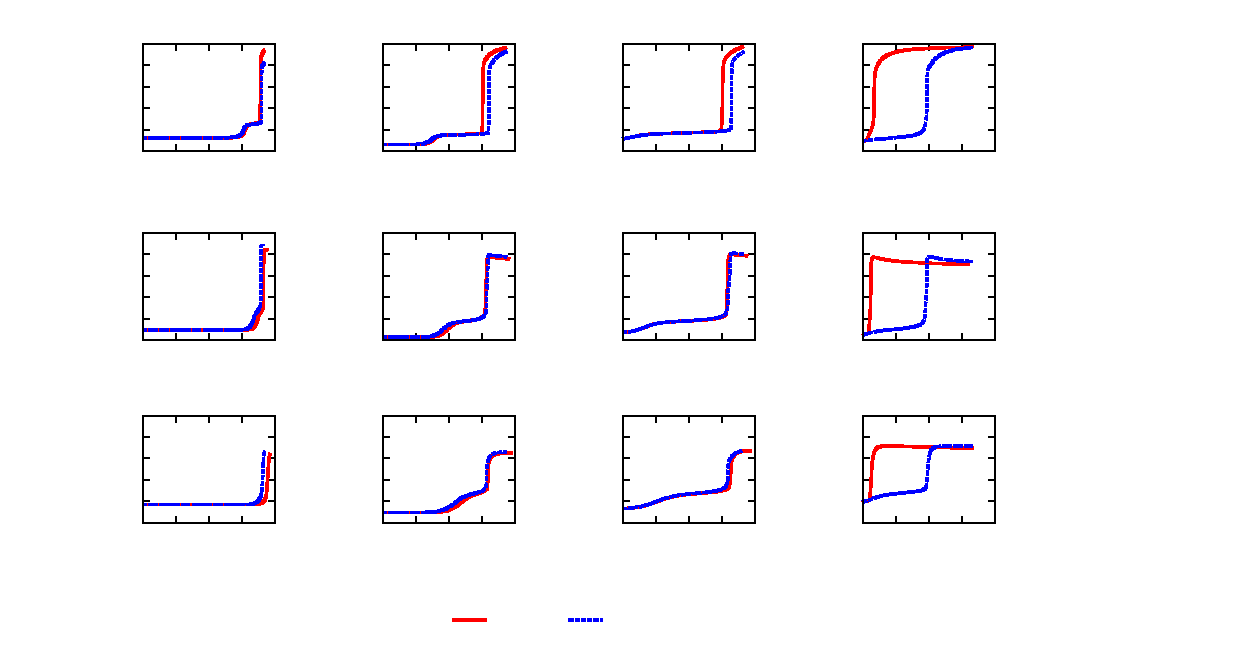
\includegraphics{LFA}}%
    \gplfronttext
  \end{picture}%
\endgroup
}
  \normalsize
  \caption{Comparison between 2D-CFD and 1D-LFA results for the steady cases with the same flow velocities but different boundary temperatures.}
  \label{fig:LFA_T}
\end{figure}

As shown in Fig.~\ref{fig:LFA_T}, two ignition stages can be seen at $Z_{\rm st}$ and $Z = 0.2$ for the $700$ K case, while at $Z = 0.3$ only one ignition dominated by low-temperature chemistry is observed, due to the reduced initial temperature.   At all three mixture fractions examined, the flamelets agree with the two-dimensional computations very well.  For the $800$ K case, both the flamelet and two-dimensional computation experience almost identical time histories, where two-stage ignition occurs at all three mixture fractions.  As the initial temperature further increases, corresponding to the increase in the boundary temperatures in the CFD computation, the two-stage ignition phenomenon is less pronounced.  However, the $900$ K case still shows good agreement between the flamelet profile with the time history of the two-dimensional computation at $Z = 0.2$ and $0.3$, while LFA slightly lags behind the CFD computation at $Z_{\rm st}$ , similar to the $800$ K case.

On the contrary, for the $1100$ K case, the ignition delay time computed with the one-dimensional flamelet assumption is significantly longer than the two-dimensional counterpart, indicating that transport processes along the mixture fraction iso-contours must be important and that autoignition is less important to the stabilization mechanism.

\subsection{Stabilization Mechanism} \label{sec:regime}

With the above analysis based on species profiles, Chemical Explosive Mode Analysis, and Lagrangian Flamelet Analysis, the transition of the stabilization mechanism and the coupling between autoignition chemistry and flame propagation can be clearly identified.  Two fundamental stabilization mechanisms are relevant: the \emph {kinetic} stabilization mechanism, due to the balance between the autoignition delay time and flow residence time, and the \emph {kinematic} stabilization mechanism, due to the balance between the local premixed flame propagation velocity and the local flow velocity.  

In this stratified composition and temperature field, autoignition and flame propagation are coupled through thermal and radical interactions, for the accumulation of the upstream radicals and heat release from autoignition accelerate the flame propagation velocity.  The flame also transfers heat and radicals through back diffusion processes to the upstream, which could also facilitate autoignition.

The stabilization mechanism was determined by comparing the two-dimensional computations with the one-dimensional inhomogeneous autoignition predicted by LFA.  When these two time history profiles agree well, the case is characterized as \emph{kinetically} stabilized.  Specifically, at $700$ K, the one-dimensional LFA agrees very well with the two-dimensional computation at all of the mixture fractions examined.  Therefore, the $700$ K case is characterized as \emph{kinetically} stabilized.  As the boundary temperature increases, the influences from premixed flame propagation become important, as predictions by LFA lag behind the CFD results for some mixture fractions.  At $800$ K, an autoignition front stabilizes the multibrachial structure at rich mixture fractions, due to the shorter ignition delay time resulting from the NTC chemistry, and a modified triple flame structure stabilizes slightly downstream of this front at leaner mixture fractions, as shown in Fig.~\ref{fig:dynamics-HRR_T}.  Further increasing the boundary temperature results in higher flame propagation velocities.  Therefore, the flame front at leaner mixture fraction depends less on radical accumulation ahead of the flame and propagates upstream, and the stabilization is influenced by both inhomogeneous autoignition and premixed flame propagation.  The transition to a \emph {kinematically} stabilized flame structure is achieved for the $1100$ K case, where the local flame propagation velocity balances the incoming flow velocity.  Therefore, the flame structure stabilizes close to the nozzle exit and depends least on radical accumulation from upstream.  Consequently, the one-dimensional LFA predictions departure from the two-dimensional computation significantly.

Based on the understanding obtained from the current study, further extension of the stabilization regime can be made, as shown in Fig.~\ref{fig:regime_T}.  For fixed inlet flow velocity, when the boundary temperature is sufficiently low, the mixture cannot be autoignited, and it is essentially a frozen flow.  Even when an external ignition source is applied, the flame cannot keep up with the excessive high flow velocity, such that the flame blows out.  When the boundary temperature is high enough to activate autoignition, it occurs far downstream, but the flame propagation velocity still cannot keep up with the flow velocity.  As a consequence, a pure \emph {kinetically} stabilized autoignition front can be achieved, which is similar to the $700$ K case.  Conversely, when the boundary temperature is sufficiently high, the flame stabilizes close to the inlet, where the upstream can be treated as frozen, due to reduced residence time, which is similar to the $1100$ K case.  Therefore, a \emph {kinematically} stabilized classical triple flame structure is achieved.  Further increase in the boundary temperature results in an attached flame with the increased flame speed.  Although not included, an attached flame was computed at $1500$ K.  In between the \emph {kinetically} and \emph {kinematically} stabilized regimes, there is a transitional regime governed by both mechanisms, which corresponds to the $800$ and $900$ K cases.  Due to the NTC behavior of the autoignition chemistry, the stabilization point, in terms of mixture fraction space, varies, and the complex multibrachial flame structure appears.  

\begin{figure}[t]
  \centering
  \scriptsize
  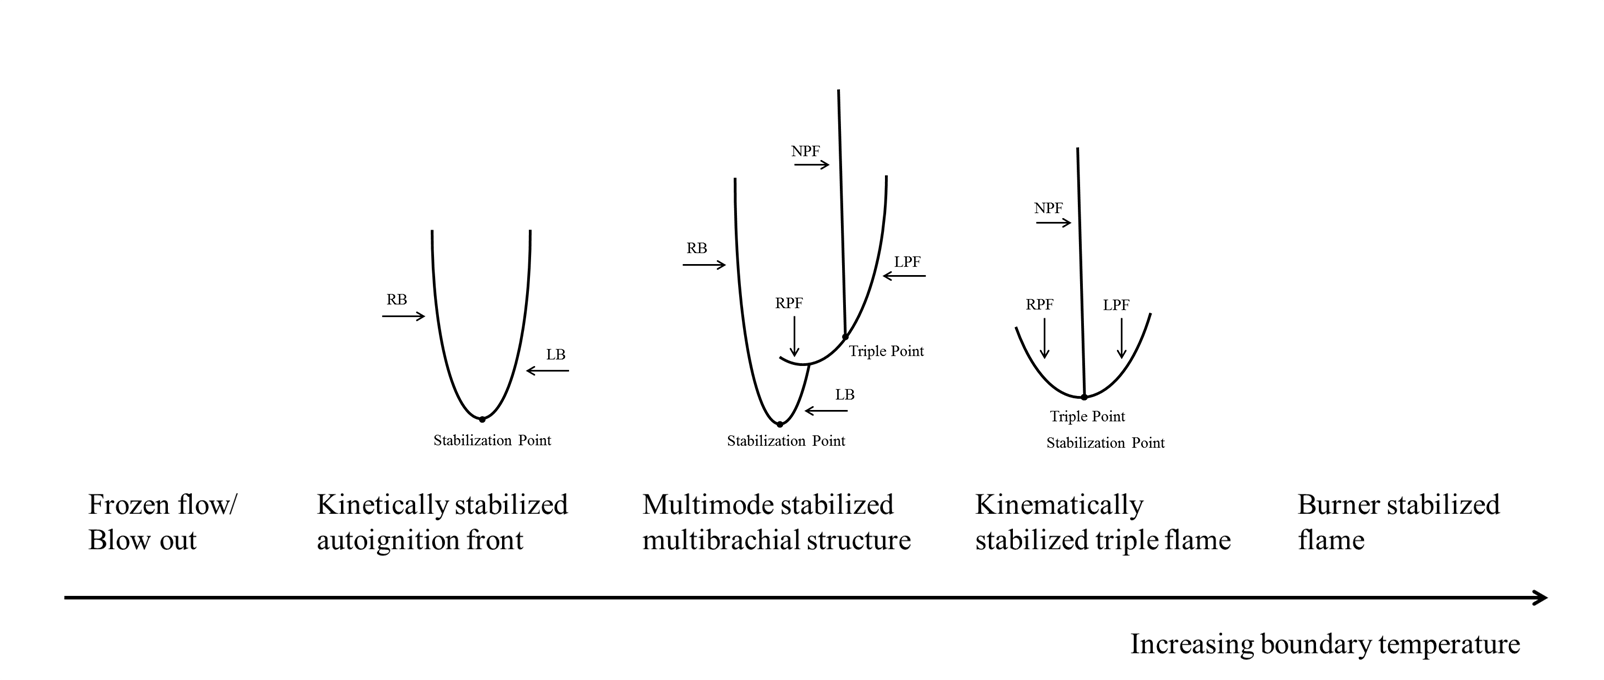
\includegraphics[width=1.0\textwidth]{ch-dynamics/regime.png}
  \normalsize
  \caption{Extended regimes of the stabilization mechanism as the coflow boundary temperature increases.}
  \label{fig:regime_T}
\end{figure}

%--------------------------------------------
\section{Flame Stabilization: Boundary Velocity Effects}\label{sec:dynamics-V}

In this section, the effect of boundary velocity and hence transport on flame stabilization is investigated.  Therefore, in all cases studied in this section, the temperature of the heated air coflow is fixed at $900$ K.  Conversely, the boundary velocities of the DME jet as well as the coflow air are varied ($2.4$, $3.2$, and $8.0$ m/s).  The dimensions of and number of grid points in the computational domain for each computation are summarized in Table~\ref{table:domain_V}.  The $3.2$ m/s case has been presented in Sec.~\ref{sec:dynamics-T}.

\begin{table*}
  \caption{Computational domain and number of grid points for steady cases with the same boundary temperature but different flow velocities.}
  \label{table:domain_V}
  \centering
  \normalsize
  \resizebox{0.6\textwidth}{!}{
  \begin{tabular}{lc*{2}{c}}
    \hline
    Inlet Velocity [m/s]& $2.4$  & $3.2$  & $8.0$   \\
    \hline
    $L_x$ [mm]& $3.5$ & $3.5$ & $15$\\
    %Coflow O.D. [mm]& $3.9$ & $3.9$ & $3.9$\\
    $N_x$ & $1536$ & $1536$  & $3072$\\
    $N_r$ & $176$ & $176$ & $176$\\
    \hline
   \end{tabular}
}
\end{table*}

\subsection{Thermal and Chemical Structure} \label{sec:dynamcis-structure_V}

The heat release rate profiles for the three cases are shown in Fig.~\ref{fig:HRR_V}.  A qualitative determination of the stabilization point is the most upstream point on the largest heat release contour (the leading point), colored by red.  The mixture fraction iso-contours of $Z_{\rm st} = 0.1005$, $Z = 0.2$, and $Z = 0.3$ are delineated in solid black lines, from right to left.

\begin{figure}[t]
  \centering
  \scriptsize
  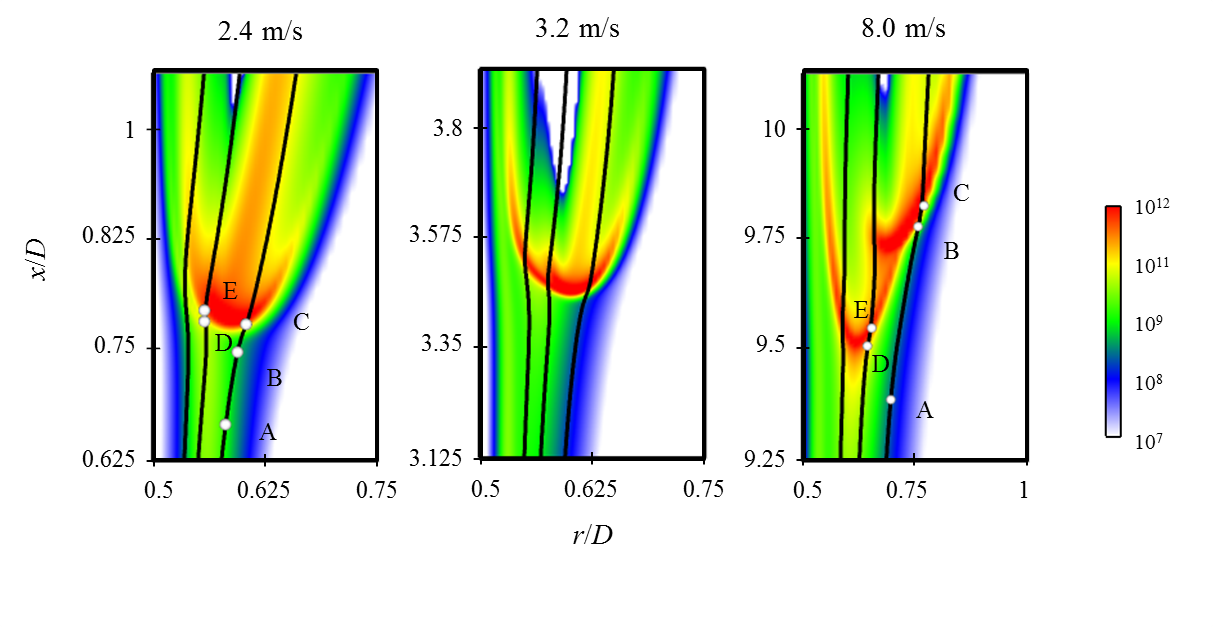
\includegraphics[width=1.0\textwidth]{ch-dynamics/HRR_V.png}
  \vspace{-0.3in}
  \normalsize
  \caption{Heat release rate [J/m$^3$-s] profiles for steady cases with the same boundary temperature but different flow velocities.  The iso-contours of $Z_{\rm st}$, $Z = 0.2$, and $Z = 0.3$ are outlined from right to left in solid lines, respectively.  The CEMA sampling points for $2.4$ and $8.0$ m/s cases are marked along the iso-contours.}
  \label{fig:HRR_V}
\end{figure}

When the inlet velocity is the lowest, $2.4$ m/s, a tribrachial thermal structure is observed very similar to that of the classical triple flame.  The triple point at $Z = 0.15$, where the three large heat release branches intersect, is also the stabilization point.  Some heat release can be found upstream of the tribrachial thermal structure for the partially reacting mixture at elevated temperature but is much less than the heat release from the flame structure.  As the inlet velocity increases to $3.2$ m/s, another branch with large heat release is found attached to the tribrachial structure around $Z = 0.2$.  The stabilization point is, again, the same as the triple point.  This structure has been analyzed in Sec.~\ref{sec:dynamics-T}.  However, as the inlet velocity further increases to $8.0$ m/s, the stabilization point is no longer on the tribrachial structure.  Instead, it is found to be near $Z = 0.25$ and is the intersection point of two trailing heat release branches.  Attached to the leaner branch, there is a tribrachial structure that appears similar to the triple flame structure.  This multibrachial structure is similar to the one discussed in Sec.~\ref{sec:dynamics-T} at a lower oxidizer temperature ($800$ K) and lower velocity ($3.2$ m/s).

Similar to Sec.~\ref{sec:diagnostics}, the controlling chemistry of the three cases was studied with CEMA.  Samplings were conducted along $Z_{\rm st}$, $Z = 0.2$, and $Z = 0.3$ iso-contours, as shown in Fig.~\ref{fig:HRR_V}.  Based on the explosive mode and participation index, the evolution of the dominant reactions is shown in Fig.~\ref{fig:CEMA_V}.

\begin{figure}
  \centering
  \scriptsize
  \resizebox{1.0\textwidth}{!}{% GNUPLOT: LaTeX picture with Postscript
\begingroup
  \makeatletter
  \providecommand\color[2][]{%
    \GenericError{(gnuplot) \space\space\space\@spaces}{%
      Package color not loaded in conjunction with
      terminal option `colourtext'%
    }{See the gnuplot documentation for explanation.%
    }{Either use 'blacktext' in gnuplot or load the package
      color.sty in LaTeX.}%
    \renewcommand\color[2][]{}%
  }%
  \providecommand\includegraphics[2][]{%
    \GenericError{(gnuplot) \space\space\space\@spaces}{%
      Package graphicx or graphics not loaded%
    }{See the gnuplot documentation for explanation.%
    }{The gnuplot epslatex terminal needs graphicx.sty or graphics.sty.}%
    \renewcommand\includegraphics[2][]{}%
  }%
  \providecommand\rotatebox[2]{#2}%
  \@ifundefined{ifGPcolor}{%
    \newif\ifGPcolor
    \GPcolortrue
  }{}%
  \@ifundefined{ifGPblacktext}{%
    \newif\ifGPblacktext
    \GPblacktexttrue
  }{}%
  % define a \g@addto@macro without @ in the name:
  \let\gplgaddtomacro\g@addto@macro
  % define empty templates for all commands taking text:
  \gdef\gplbacktext{}%
  \gdef\gplfronttext{}%
  \makeatother
  \ifGPblacktext
    % no textcolor at all
    \def\colorrgb#1{}%
    \def\colorgray#1{}%
  \else
    % gray or color?
    \ifGPcolor
      \def\colorrgb#1{\color[rgb]{#1}}%
      \def\colorgray#1{\color[gray]{#1}}%
      \expandafter\def\csname LTw\endcsname{\color{white}}%
      \expandafter\def\csname LTb\endcsname{\color{black}}%
      \expandafter\def\csname LTa\endcsname{\color{black}}%
      \expandafter\def\csname LT0\endcsname{\color[rgb]{1,0,0}}%
      \expandafter\def\csname LT1\endcsname{\color[rgb]{0,1,0}}%
      \expandafter\def\csname LT2\endcsname{\color[rgb]{0,0,1}}%
      \expandafter\def\csname LT3\endcsname{\color[rgb]{1,0,1}}%
      \expandafter\def\csname LT4\endcsname{\color[rgb]{0,1,1}}%
      \expandafter\def\csname LT5\endcsname{\color[rgb]{1,1,0}}%
      \expandafter\def\csname LT6\endcsname{\color[rgb]{0,0,0}}%
      \expandafter\def\csname LT7\endcsname{\color[rgb]{1,0.3,0}}%
      \expandafter\def\csname LT8\endcsname{\color[rgb]{0.5,0.5,0.5}}%
    \else
      % gray
      \def\colorrgb#1{\color{black}}%
      \def\colorgray#1{\color[gray]{#1}}%
      \expandafter\def\csname LTw\endcsname{\color{white}}%
      \expandafter\def\csname LTb\endcsname{\color{black}}%
      \expandafter\def\csname LTa\endcsname{\color{black}}%
      \expandafter\def\csname LT0\endcsname{\color{black}}%
      \expandafter\def\csname LT1\endcsname{\color{black}}%
      \expandafter\def\csname LT2\endcsname{\color{black}}%
      \expandafter\def\csname LT3\endcsname{\color{black}}%
      \expandafter\def\csname LT4\endcsname{\color{black}}%
      \expandafter\def\csname LT5\endcsname{\color{black}}%
      \expandafter\def\csname LT6\endcsname{\color{black}}%
      \expandafter\def\csname LT7\endcsname{\color{black}}%
      \expandafter\def\csname LT8\endcsname{\color{black}}%
    \fi
  \fi
  \setlength{\unitlength}{0.0500bp}%
  \begin{picture}(7200.00,5040.00)%
    \gplgaddtomacro\gplbacktext{%
      \csname LTb\endcsname%
      \put(2748,1043){\makebox(0,0)[r]{\strut{}CH$_3$OCH$_2$+O$_2$$\Longleftrightarrow$CH$_3$OCH$_2$O$_2$}}%
      \put(2748,1383){\makebox(0,0)[r]{\strut{}CH$_2$OCH$_2$O$_2$H$\Longleftrightarrow$OH+CH$_2$O+CH$_2$O}}%
      \put(2748,1722){\makebox(0,0)[r]{\strut{}CH$_3$OCH$_3$+OH$\Longleftrightarrow$CH$_3$OCH$_2$+H$_2$O}}%
      \put(2748,2061){\makebox(0,0)[r]{\strut{}H+O$_2$+M$\Longleftrightarrow$HO$_2$+M}}%
      \put(2748,2400){\makebox(0,0)[r]{\strut{}HCO+O$_2$$\Longleftrightarrow$CO+HO$_2$}}%
      \put(2748,2740){\makebox(0,0)[r]{\strut{}CH$_3$OCH$_2$O$_2$$\Longleftrightarrow$CH$_2$OCH$_2$O$_2$H}}%
      \put(2748,3079){\makebox(0,0)[r]{\strut{}CH$_2$O+OH$\Longleftrightarrow$HCO+H$_2$O}}%
      \put(2748,3418){\makebox(0,0)[r]{\strut{}HO$_2$CH$_2$OCHO$\Longleftrightarrow$OCH$_2$OCHO+OH}}%
      \put(2748,3757){\makebox(0,0)[r]{\strut{}CH$_2$O+H$\Longleftrightarrow$HCO+H$_2$}}%
      \put(2748,4097){\makebox(0,0)[r]{\strut{}CH$_3$OCH$_3$+H$\Longleftrightarrow$CH$_3$OCH$_2$+H$_2$}}%
      \put(2748,4436){\makebox(0,0)[r]{\strut{}H+O$_2$$\Longleftrightarrow$O+OH}}%
      \put(2880,484){\makebox(0,0){\strut{}-1}}%
      \put(3861,484){\makebox(0,0){\strut{}-0.5}}%
      \put(4842,484){\makebox(0,0){\strut{} 0}}%
      \put(5822,484){\makebox(0,0){\strut{} 0.5}}%
      \put(6803,484){\makebox(0,0){\strut{} 1}}%
      \csname LTb\endcsname%
      \put(4841,154){\makebox(0,0){\strut{}Normalized Participation Index}}%
      \put(5234,1332){\makebox(0,0)[l]{\strut{}Point A}}%
      \put(5234,1501){\makebox(0,0)[l]{\strut{}Point B}}%
      \put(5234,1688){\makebox(0,0)[l]{\strut{}Point C}}%
      \put(5234,1857){\makebox(0,0)[l]{\strut{}Point D}}%
      \put(5234,2027){\makebox(0,0)[l]{\strut{}Point E}}%
      \put(5234,2231){\makebox(0,0)[l]{\strut{}$2.4$ m/s}}%
    }%
    \gplgaddtomacro\gplfronttext{%
      \csname LTb\endcsname%
      \put(5690,1337){\makebox(0,0)[r]{\strut{} }}%
      \csname LTb\endcsname%
      \put(5690,1513){\makebox(0,0)[r]{\strut{} }}%
      \csname LTb\endcsname%
      \put(5690,1689){\makebox(0,0)[r]{\strut{} }}%
      \csname LTb\endcsname%
      \put(5690,1865){\makebox(0,0)[r]{\strut{} }}%
      \csname LTb\endcsname%
      \put(5690,2041){\makebox(0,0)[r]{\strut{} }}%
    }%
    \gplbacktext
    \put(0,0){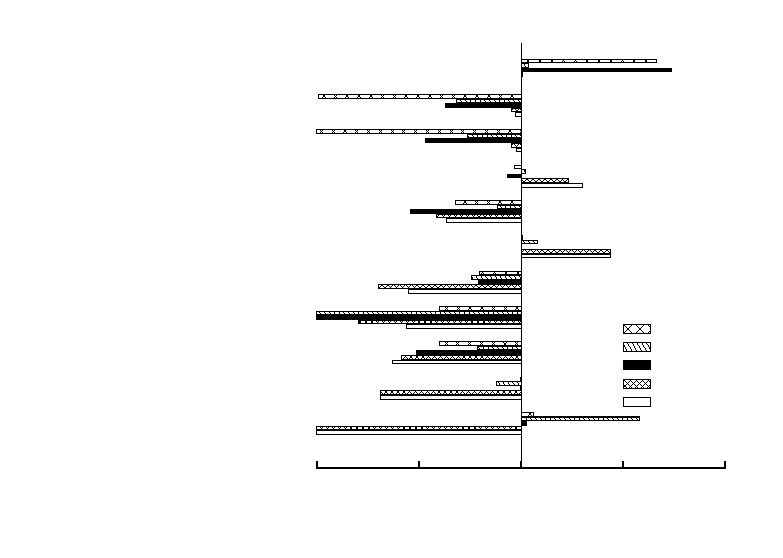
\includegraphics{ch-dynamics/CEMA_24}}%
    \gplfronttext
  \end{picture}%
\endgroup
}
  \resizebox{1.0\textwidth}{!}{% GNUPLOT: LaTeX picture with Postscript
\begingroup
  \makeatletter
  \providecommand\color[2][]{%
    \GenericError{(gnuplot) \space\space\space\@spaces}{%
      Package color not loaded in conjunction with
      terminal option `colourtext'%
    }{See the gnuplot documentation for explanation.%
    }{Either use 'blacktext' in gnuplot or load the package
      color.sty in LaTeX.}%
    \renewcommand\color[2][]{}%
  }%
  \providecommand\includegraphics[2][]{%
    \GenericError{(gnuplot) \space\space\space\@spaces}{%
      Package graphicx or graphics not loaded%
    }{See the gnuplot documentation for explanation.%
    }{The gnuplot epslatex terminal needs graphicx.sty or graphics.sty.}%
    \renewcommand\includegraphics[2][]{}%
  }%
  \providecommand\rotatebox[2]{#2}%
  \@ifundefined{ifGPcolor}{%
    \newif\ifGPcolor
    \GPcolortrue
  }{}%
  \@ifundefined{ifGPblacktext}{%
    \newif\ifGPblacktext
    \GPblacktexttrue
  }{}%
  % define a \g@addto@macro without @ in the name:
  \let\gplgaddtomacro\g@addto@macro
  % define empty templates for all commands taking text:
  \gdef\gplbacktext{}%
  \gdef\gplfronttext{}%
  \makeatother
  \ifGPblacktext
    % no textcolor at all
    \def\colorrgb#1{}%
    \def\colorgray#1{}%
  \else
    % gray or color?
    \ifGPcolor
      \def\colorrgb#1{\color[rgb]{#1}}%
      \def\colorgray#1{\color[gray]{#1}}%
      \expandafter\def\csname LTw\endcsname{\color{white}}%
      \expandafter\def\csname LTb\endcsname{\color{black}}%
      \expandafter\def\csname LTa\endcsname{\color{black}}%
      \expandafter\def\csname LT0\endcsname{\color[rgb]{1,0,0}}%
      \expandafter\def\csname LT1\endcsname{\color[rgb]{0,1,0}}%
      \expandafter\def\csname LT2\endcsname{\color[rgb]{0,0,1}}%
      \expandafter\def\csname LT3\endcsname{\color[rgb]{1,0,1}}%
      \expandafter\def\csname LT4\endcsname{\color[rgb]{0,1,1}}%
      \expandafter\def\csname LT5\endcsname{\color[rgb]{1,1,0}}%
      \expandafter\def\csname LT6\endcsname{\color[rgb]{0,0,0}}%
      \expandafter\def\csname LT7\endcsname{\color[rgb]{1,0.3,0}}%
      \expandafter\def\csname LT8\endcsname{\color[rgb]{0.5,0.5,0.5}}%
    \else
      % gray
      \def\colorrgb#1{\color{black}}%
      \def\colorgray#1{\color[gray]{#1}}%
      \expandafter\def\csname LTw\endcsname{\color{white}}%
      \expandafter\def\csname LTb\endcsname{\color{black}}%
      \expandafter\def\csname LTa\endcsname{\color{black}}%
      \expandafter\def\csname LT0\endcsname{\color{black}}%
      \expandafter\def\csname LT1\endcsname{\color{black}}%
      \expandafter\def\csname LT2\endcsname{\color{black}}%
      \expandafter\def\csname LT3\endcsname{\color{black}}%
      \expandafter\def\csname LT4\endcsname{\color{black}}%
      \expandafter\def\csname LT5\endcsname{\color{black}}%
      \expandafter\def\csname LT6\endcsname{\color{black}}%
      \expandafter\def\csname LT7\endcsname{\color{black}}%
      \expandafter\def\csname LT8\endcsname{\color{black}}%
    \fi
  \fi
  \setlength{\unitlength}{0.0500bp}%
  \begin{picture}(7200.00,5040.00)%
    \gplgaddtomacro\gplbacktext{%
      \csname LTb\endcsname%
      \put(2748,1043){\makebox(0,0)[r]{\strut{}H$_2$O$_2$+M$\Longleftrightarrow$OH+OH+M}}%
      \put(2748,1383){\makebox(0,0)[r]{\strut{}HCO+O$_2$$\Longleftrightarrow$CO+HO$_2$}}%
      \put(2748,1722){\makebox(0,0)[r]{\strut{}CH$_2$O+OH$\Longleftrightarrow$HCO+H$_2$O}}%
      \put(2748,2061){\makebox(0,0)[r]{\strut{}HO$_2$+HO$_2$$\Longleftrightarrow$H$_2$O$_2$+O$_2$}}%
      \put(2748,2400){\makebox(0,0)[r]{\strut{}CH$_3$OCH$_3$+HO$_2$$\Longleftrightarrow$CH$_3$OCH$_2$+H$_2$O$_2$}}%
      \put(2748,2740){\makebox(0,0)[r]{\strut{}CH$_3$OCH$_2$O$_2$$\Longleftrightarrow$CH$_2$OCH$_2$O$_2$H}}%
      \put(2748,3079){\makebox(0,0)[r]{\strut{}CH$_2$OCH$_2$O$_2$H$\Longleftrightarrow$OH+CH$_2$O+CH$_2$O}}%
      \put(2748,3418){\makebox(0,0)[r]{\strut{}CH$_3$OCH$_2$+O$_2$$\Longleftrightarrow$CH$_3$OCH$_2$O$_2$}}%
      \put(2748,3757){\makebox(0,0)[r]{\strut{}CH$_2$O+HO$_2$$\Longleftrightarrow$HCO+H$_2$O$_2$}}%
      \put(2748,4097){\makebox(0,0)[r]{\strut{}H+O$_2$+M$\Longleftrightarrow$HO$_2$+M}}%
      \put(2748,4436){\makebox(0,0)[r]{\strut{}H+O$_2$$\Longleftrightarrow$O+OH}}%
      \put(2880,484){\makebox(0,0){\strut{}-1}}%
      \put(3861,484){\makebox(0,0){\strut{}-0.5}}%
      \put(4842,484){\makebox(0,0){\strut{} 0}}%
      \put(5822,484){\makebox(0,0){\strut{} 0.5}}%
      \put(6803,484){\makebox(0,0){\strut{} 1}}%
      \csname LTb\endcsname%
      \put(4841,154){\makebox(0,0){\strut{}Normalized Participation Index}}%
      \put(5234,1332){\makebox(0,0)[l]{\strut{}Point A}}%
      \put(5234,1501){\makebox(0,0)[l]{\strut{}Point B}}%
      \put(5234,1688){\makebox(0,0)[l]{\strut{}Point C}}%
      \put(5234,1857){\makebox(0,0)[l]{\strut{}Point D}}%
      \put(5234,2027){\makebox(0,0)[l]{\strut{}Point E}}%
      \put(5234,2231){\makebox(0,0)[l]{\strut{}$8.0$ m/s}}%
    }%
    \gplgaddtomacro\gplfronttext{%
      \csname LTb\endcsname%
      \put(5690,1337){\makebox(0,0)[r]{\strut{} }}%
      \csname LTb\endcsname%
      \put(5690,1513){\makebox(0,0)[r]{\strut{} }}%
      \csname LTb\endcsname%
      \put(5690,1689){\makebox(0,0)[r]{\strut{} }}%
      \csname LTb\endcsname%
      \put(5690,1865){\makebox(0,0)[r]{\strut{} }}%
      \csname LTb\endcsname%
      \put(5690,2041){\makebox(0,0)[r]{\strut{} }}%
    }%
    \gplbacktext
    \put(0,0){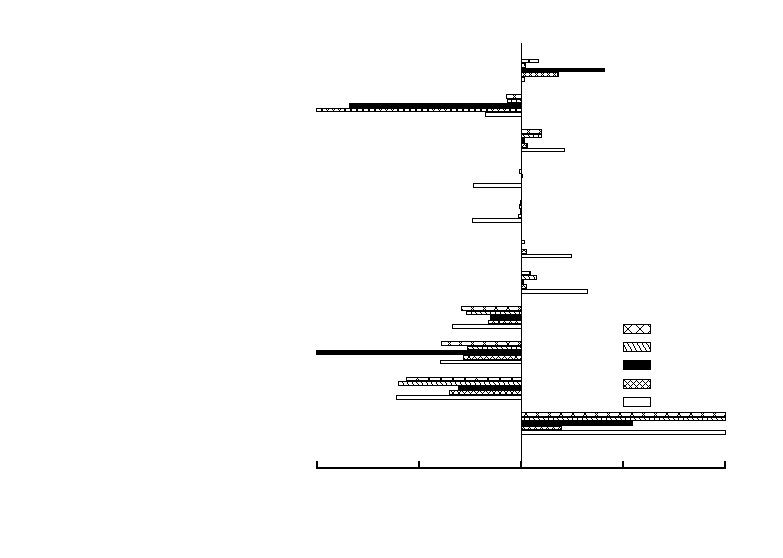
\includegraphics{ch-dynamics/CEMA_80}}%
    \gplfronttext
  \end{picture}%
\endgroup
}
  \normalsize
  \caption{Normalized participation index at $2.4$ and $8.0$ m/s.  Sampled locations are delineated in Fig.~\ref{fig:HRR_V}.}
  \label{fig:CEMA_V}
\end{figure}

At $2.4$ m/s, the dominant reactions along $Z_{\rm st}$ and $Z = 0.2$ iso-contours evolve in similar ways: upstream of the tribrachial structure (points A, B, and D), low-temperature chemistry, characterized by reactions involving CH$_3$OCH$_2$O$_2$ radicals, is active.  Due to the high diffusivity of H radicals and the elevated pressure, the H radical recombination reaction (H + O$_2$ + M $\Longleftrightarrow$ HO$_2$ + M) is important.  At the most reactive region (points C and E), the H radical branching reaction (H + O$_2$ $\Longleftrightarrow$ O + OH) becomes the most important chain branching reaction, indicating the transition to high-temperature chemistry.  On the contrary, for the $8.0$ m/s case, while low-temperature chemistry is still active upstream of the multibrachial structure, the dominant chain branching reaction is the hydrogen peroxide branching reaction (H$_2$O$_2$ + M $\Longleftrightarrow$ OH + OH + M).  Moreover, the dominant reactions along the $Z_{\rm st}$ and $Z = 0.2$ iso-contours evolve in different ways.  Along the $Z = 0.2$ iso-contour, from point D to E, the hydrogen peroxide branching reaction is always the dominant reaction, indicating the role of low-to-intermediate temperature autoignition chemistry~\cite{westbrook00}.  Although this is the case at point A on the $Z_{\rm st}$ iso-contour, the H radical chain branching reaction becomes dominant at point C, the most reactive zone, indicating that the dominant chemical pathway shifts to high-temperature chemistry.  CEMA results for the $3.2$ m/s case show similar transitions as those of the $8.0$ m/s case, although their thermal structures appear different.  Therefore, further computational diagnostics is needed to identify the dominant combustion mode.

\subsection{Stabilization Mechanism} 

Similar to the Lagrangian analysis presented in Sec.~\ref{sec:diagnostics}, the Lagrangian time history profiles of the two-dimensional computation and one-dimensional LFA are shown in Fig.~\ref{fig:LFA_V}.  For each inlet velocity case, the temperature profiles are compared along $Z_{\rm st}$, $Z = 0.2$, and $Z = 0.3$.

\begin{figure}
  \centering
  \scriptsize
  \resizebox{1.0\textwidth}{!}{% GNUPLOT: LaTeX picture with Postscript
\begingroup
  \makeatletter
  \providecommand\color[2][]{%
    \GenericError{(gnuplot) \space\space\space\@spaces}{%
      Package color not loaded in conjunction with
      terminal option `colourtext'%
    }{See the gnuplot documentation for explanation.%
    }{Either use 'blacktext' in gnuplot or load the package
      color.sty in LaTeX.}%
    \renewcommand\color[2][]{}%
  }%
  \providecommand\includegraphics[2][]{%
    \GenericError{(gnuplot) \space\space\space\@spaces}{%
      Package graphicx or graphics not loaded%
    }{See the gnuplot documentation for explanation.%
    }{The gnuplot epslatex terminal needs graphicx.sty or graphics.sty.}%
    \renewcommand\includegraphics[2][]{}%
  }%
  \providecommand\rotatebox[2]{#2}%
  \@ifundefined{ifGPcolor}{%
    \newif\ifGPcolor
    \GPcolortrue
  }{}%
  \@ifundefined{ifGPblacktext}{%
    \newif\ifGPblacktext
    \GPblacktexttrue
  }{}%
  % define a \g@addto@macro without @ in the name:
  \let\gplgaddtomacro\g@addto@macro
  % define empty templates for all commands taking text:
  \gdef\gplbacktext{}%
  \gdef\gplfronttext{}%
  \makeatother
  \ifGPblacktext
    % no textcolor at all
    \def\colorrgb#1{}%
    \def\colorgray#1{}%
  \else
    % gray or color?
    \ifGPcolor
      \def\colorrgb#1{\color[rgb]{#1}}%
      \def\colorgray#1{\color[gray]{#1}}%
      \expandafter\def\csname LTw\endcsname{\color{white}}%
      \expandafter\def\csname LTb\endcsname{\color{black}}%
      \expandafter\def\csname LTa\endcsname{\color{black}}%
      \expandafter\def\csname LT0\endcsname{\color[rgb]{1,0,0}}%
      \expandafter\def\csname LT1\endcsname{\color[rgb]{0,1,0}}%
      \expandafter\def\csname LT2\endcsname{\color[rgb]{0,0,1}}%
      \expandafter\def\csname LT3\endcsname{\color[rgb]{1,0,1}}%
      \expandafter\def\csname LT4\endcsname{\color[rgb]{0,1,1}}%
      \expandafter\def\csname LT5\endcsname{\color[rgb]{1,1,0}}%
      \expandafter\def\csname LT6\endcsname{\color[rgb]{0,0,0}}%
      \expandafter\def\csname LT7\endcsname{\color[rgb]{1,0.3,0}}%
      \expandafter\def\csname LT8\endcsname{\color[rgb]{0.5,0.5,0.5}}%
    \else
      % gray
      \def\colorrgb#1{\color{black}}%
      \def\colorgray#1{\color[gray]{#1}}%
      \expandafter\def\csname LTw\endcsname{\color{white}}%
      \expandafter\def\csname LTb\endcsname{\color{black}}%
      \expandafter\def\csname LTa\endcsname{\color{black}}%
      \expandafter\def\csname LT0\endcsname{\color{black}}%
      \expandafter\def\csname LT1\endcsname{\color{black}}%
      \expandafter\def\csname LT2\endcsname{\color{black}}%
      \expandafter\def\csname LT3\endcsname{\color{black}}%
      \expandafter\def\csname LT4\endcsname{\color{black}}%
      \expandafter\def\csname LT5\endcsname{\color{black}}%
      \expandafter\def\csname LT6\endcsname{\color{black}}%
      \expandafter\def\csname LT7\endcsname{\color{black}}%
      \expandafter\def\csname LT8\endcsname{\color{black}}%
    \fi
  \fi
  \setlength{\unitlength}{0.0500bp}%
  \begin{picture}(8640.00,6048.00)%
    \gplgaddtomacro\gplbacktext{%
      \csname LTb\endcsname%
      \put(6694,4756){\makebox(0,0)[r]{\strut{} 800}}%
      \put(6694,4961){\makebox(0,0)[r]{\strut{} 1200}}%
      \put(6694,5167){\makebox(0,0)[r]{\strut{} 1600}}%
      \put(6694,5372){\makebox(0,0)[r]{\strut{} 2000}}%
      \put(6694,5578){\makebox(0,0)[r]{\strut{} 2400}}%
      \put(6694,5783){\makebox(0,0)[r]{\strut{} 2800}}%
      \put(6826,4536){\makebox(0,0){\strut{} 0}}%
      \put(7137,4536){\makebox(0,0){\strut{} 0.5}}%
      \put(7448,4536){\makebox(0,0){\strut{} 1}}%
      \put(7759,4536){\makebox(0,0){\strut{} 1.5}}%
      \put(8070,4536){\makebox(0,0){\strut{} 2}}%
      \put(5792,5269){\rotatebox{-270}{\makebox(0,0){\strut{}\vspace{-36pt}$T$ [K]}}}%
      \put(7448,4206){\makebox(0,0){\strut{}\vspace{12pt}Time [ms]}}%
      \put(1987,6047){\makebox(0,0)[l]{\strut{}$2.4$ m/s}}%
      \put(4579,6047){\makebox(0,0)[l]{\strut{}$3.2$ m/s}}%
      \put(7170,6047){\makebox(0,0)[l]{\strut{}$8.0$ m/s}}%
      \put(-172,1633){\makebox(0,0)[l]{\strut{}$Z = 0.3$}}%
      \put(-172,3447){\makebox(0,0)[l]{\strut{}$Z = 0.2$}}%
      \put(-172,5261){\makebox(0,0)[l]{\strut{}$Z = Z_{\rm st}$}}%
    }%
    \gplgaddtomacro\gplfronttext{%
    }%
    \gplgaddtomacro\gplbacktext{%
      \csname LTb\endcsname%
      \put(6694,2941){\makebox(0,0)[r]{\strut{} 600}}%
      \put(6694,3147){\makebox(0,0)[r]{\strut{} 1000}}%
      \put(6694,3352){\makebox(0,0)[r]{\strut{} 1400}}%
      \put(6694,3558){\makebox(0,0)[r]{\strut{} 1800}}%
      \put(6694,3763){\makebox(0,0)[r]{\strut{} 2200}}%
      \put(6694,3969){\makebox(0,0)[r]{\strut{} 2600}}%
      \put(6826,2721){\makebox(0,0){\strut{} 0}}%
      \put(7137,2721){\makebox(0,0){\strut{} 0.5}}%
      \put(7448,2721){\makebox(0,0){\strut{} 1}}%
      \put(7759,2721){\makebox(0,0){\strut{} 1.5}}%
      \put(8070,2721){\makebox(0,0){\strut{} 2}}%
      \put(5792,3455){\rotatebox{-270}{\makebox(0,0){\strut{}\vspace{-36pt}$T$ [K]}}}%
      \put(7448,2391){\makebox(0,0){\strut{}\vspace{12pt}Time [ms]}}%
    }%
    \gplgaddtomacro\gplfronttext{%
    }%
    \gplgaddtomacro\gplbacktext{%
      \csname LTb\endcsname%
      \put(6694,1187){\makebox(0,0)[r]{\strut{} 400}}%
      \put(6694,1393){\makebox(0,0)[r]{\strut{} 800}}%
      \put(6694,1598){\makebox(0,0)[r]{\strut{} 1200}}%
      \put(6694,1804){\makebox(0,0)[r]{\strut{} 1600}}%
      \put(6694,2009){\makebox(0,0)[r]{\strut{} 2000}}%
      \put(6694,2215){\makebox(0,0)[r]{\strut{} 2400}}%
      \put(6826,967){\makebox(0,0){\strut{} 0}}%
      \put(7137,967){\makebox(0,0){\strut{} 0.5}}%
      \put(7448,967){\makebox(0,0){\strut{} 1}}%
      \put(7759,967){\makebox(0,0){\strut{} 1.5}}%
      \put(8070,967){\makebox(0,0){\strut{} 2}}%
      \put(5792,1701){\rotatebox{-270}{\makebox(0,0){\strut{}\vspace{-36pt}$T$ [K]}}}%
      \put(7448,637){\makebox(0,0){\strut{}\vspace{12pt}Time [ms]}}%
    }%
    \gplgaddtomacro\gplfronttext{%
    }%
    \gplgaddtomacro\gplbacktext{%
      \csname LTb\endcsname%
      \put(4102,4756){\makebox(0,0)[r]{\strut{} 800}}%
      \put(4102,4961){\makebox(0,0)[r]{\strut{} 1200}}%
      \put(4102,5167){\makebox(0,0)[r]{\strut{} 1600}}%
      \put(4102,5372){\makebox(0,0)[r]{\strut{} 2000}}%
      \put(4102,5578){\makebox(0,0)[r]{\strut{} 2400}}%
      \put(4102,5783){\makebox(0,0)[r]{\strut{} 2800}}%
      \put(4234,4536){\makebox(0,0){\strut{} 0}}%
      \put(4545,4536){\makebox(0,0){\strut{} 0.3}}%
      \put(4856,4536){\makebox(0,0){\strut{} 0.6}}%
      \put(5167,4536){\makebox(0,0){\strut{} 0.9}}%
      \put(5478,4536){\makebox(0,0){\strut{} 1.2}}%
      \put(3200,5269){\rotatebox{-270}{\makebox(0,0){\strut{}\vspace{-36pt}$T$ [K]}}}%
      \put(4856,4206){\makebox(0,0){\strut{}\vspace{12pt}Time [ms]}}%
    }%
    \gplgaddtomacro\gplfronttext{%
    }%
    \gplgaddtomacro\gplbacktext{%
      \csname LTb\endcsname%
      \put(4102,2941){\makebox(0,0)[r]{\strut{} 600}}%
      \put(4102,3147){\makebox(0,0)[r]{\strut{} 1000}}%
      \put(4102,3352){\makebox(0,0)[r]{\strut{} 1400}}%
      \put(4102,3558){\makebox(0,0)[r]{\strut{} 1800}}%
      \put(4102,3763){\makebox(0,0)[r]{\strut{} 2200}}%
      \put(4102,3969){\makebox(0,0)[r]{\strut{} 2600}}%
      \put(4234,2721){\makebox(0,0){\strut{} 0}}%
      \put(4545,2721){\makebox(0,0){\strut{} 0.3}}%
      \put(4856,2721){\makebox(0,0){\strut{} 0.6}}%
      \put(5167,2721){\makebox(0,0){\strut{} 0.9}}%
      \put(5478,2721){\makebox(0,0){\strut{} 1.2}}%
      \put(3200,3455){\rotatebox{-270}{\makebox(0,0){\strut{}\vspace{-36pt}$T$ [K]}}}%
      \put(4856,2391){\makebox(0,0){\strut{}\vspace{12pt}Time [ms]}}%
    }%
    \gplgaddtomacro\gplfronttext{%
    }%
    \gplgaddtomacro\gplbacktext{%
      \csname LTb\endcsname%
      \put(4102,1187){\makebox(0,0)[r]{\strut{} 400}}%
      \put(4102,1393){\makebox(0,0)[r]{\strut{} 800}}%
      \put(4102,1598){\makebox(0,0)[r]{\strut{} 1200}}%
      \put(4102,1804){\makebox(0,0)[r]{\strut{} 1600}}%
      \put(4102,2009){\makebox(0,0)[r]{\strut{} 2000}}%
      \put(4102,2215){\makebox(0,0)[r]{\strut{} 2400}}%
      \put(4234,967){\makebox(0,0){\strut{} 0}}%
      \put(4545,967){\makebox(0,0){\strut{} 0.3}}%
      \put(4856,967){\makebox(0,0){\strut{} 0.6}}%
      \put(5167,967){\makebox(0,0){\strut{} 0.9}}%
      \put(5478,967){\makebox(0,0){\strut{} 1.2}}%
      \put(3200,1701){\rotatebox{-270}{\makebox(0,0){\strut{}\vspace{-36pt}$T$ [K]}}}%
      \put(4856,637){\makebox(0,0){\strut{}\vspace{12pt}Time [ms]}}%
    }%
    \gplgaddtomacro\gplfronttext{%
    }%
    \gplgaddtomacro\gplbacktext{%
      \csname LTb\endcsname%
      \put(1510,4756){\makebox(0,0)[r]{\strut{} 800}}%
      \put(1510,4961){\makebox(0,0)[r]{\strut{} 1200}}%
      \put(1510,5167){\makebox(0,0)[r]{\strut{} 1600}}%
      \put(1510,5372){\makebox(0,0)[r]{\strut{} 2000}}%
      \put(1510,5578){\makebox(0,0)[r]{\strut{} 2400}}%
      \put(1510,5783){\makebox(0,0)[r]{\strut{} 2800}}%
      \put(1642,4536){\makebox(0,0){\strut{} 0}}%
      \put(1953,4536){\makebox(0,0){\strut{} 0.3}}%
      \put(2264,4536){\makebox(0,0){\strut{} 0.6}}%
      \put(2575,4536){\makebox(0,0){\strut{} 0.9}}%
      \put(2886,4536){\makebox(0,0){\strut{} 1.2}}%
      \put(608,5269){\rotatebox{-270}{\makebox(0,0){\strut{}\vspace{-36pt}$T$ [K]}}}%
      \put(2264,4206){\makebox(0,0){\strut{}\vspace{12pt}Time [ms]}}%
    }%
    \gplgaddtomacro\gplfronttext{%
    }%
    \gplgaddtomacro\gplbacktext{%
      \csname LTb\endcsname%
      \put(1510,2941){\makebox(0,0)[r]{\strut{} 600}}%
      \put(1510,3147){\makebox(0,0)[r]{\strut{} 1000}}%
      \put(1510,3352){\makebox(0,0)[r]{\strut{} 1400}}%
      \put(1510,3558){\makebox(0,0)[r]{\strut{} 1800}}%
      \put(1510,3763){\makebox(0,0)[r]{\strut{} 2200}}%
      \put(1510,3969){\makebox(0,0)[r]{\strut{} 2600}}%
      \put(1642,2721){\makebox(0,0){\strut{} 0}}%
      \put(1953,2721){\makebox(0,0){\strut{} 0.3}}%
      \put(2264,2721){\makebox(0,0){\strut{} 0.6}}%
      \put(2575,2721){\makebox(0,0){\strut{} 0.9}}%
      \put(2886,2721){\makebox(0,0){\strut{} 1.2}}%
      \put(608,3455){\rotatebox{-270}{\makebox(0,0){\strut{}\vspace{-36pt}$T$ [K]}}}%
      \put(2264,2391){\makebox(0,0){\strut{}\vspace{12pt}Time [ms]}}%
    }%
    \gplgaddtomacro\gplfronttext{%
    }%
    \gplgaddtomacro\gplbacktext{%
      \csname LTb\endcsname%
      \put(1510,1187){\makebox(0,0)[r]{\strut{} 400}}%
      \put(1510,1393){\makebox(0,0)[r]{\strut{} 800}}%
      \put(1510,1598){\makebox(0,0)[r]{\strut{} 1200}}%
      \put(1510,1804){\makebox(0,0)[r]{\strut{} 1600}}%
      \put(1510,2009){\makebox(0,0)[r]{\strut{} 2000}}%
      \put(1510,2215){\makebox(0,0)[r]{\strut{} 2400}}%
      \put(1642,967){\makebox(0,0){\strut{} 0}}%
      \put(1953,967){\makebox(0,0){\strut{} 0.3}}%
      \put(2264,967){\makebox(0,0){\strut{} 0.6}}%
      \put(2575,967){\makebox(0,0){\strut{} 0.9}}%
      \put(2886,967){\makebox(0,0){\strut{} 1.2}}%
      \put(608,1701){\rotatebox{-270}{\makebox(0,0){\strut{}\vspace{-36pt}$T$ [K]}}}%
      \put(2264,637){\makebox(0,0){\strut{}\vspace{12pt}Time [ms]}}%
      \put(4147,242){\makebox(0,0)[l]{\strut{}2D-CFD}}%
      \put(5270,242){\makebox(0,0)[l]{\strut{}1D-LFA}}%
    }%
    \gplgaddtomacro\gplfronttext{%
      \csname LTb\endcsname%
      \put(3646,253){\makebox(0,0)[r]{\strut{} }}%
      \csname LTb\endcsname%
      \put(4765,253){\makebox(0,0)[r]{\strut{}    }}%
    }%
    \gplbacktext
    \put(0,0){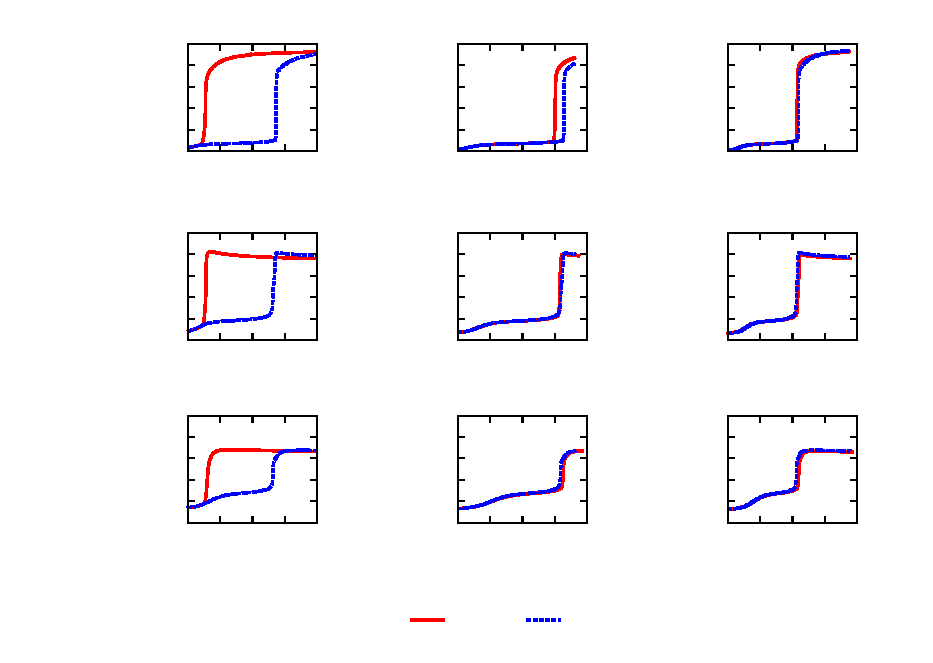
\includegraphics{ch-dynamics/LFA_V}}%
    \gplfronttext
  \end{picture}%
\endgroup
}
  \normalsize
  \caption{Comparison between 2D-CFD and 1D-LFA results for the steady cases with the same boundary temperature but different flow velocities.}
  \label{fig:LFA_V}
\end{figure}

For the $2.4$ m/s case, LFA fails to match the two-dimensional result at all three mixture fractions, indicating that transport processes normal to the mixture fraction gradient are crucial, which further indicates that flame propagation is the dominant stabilization mechanism.  At $3.2$ m/s, LFA slightly lags behind the two-dimensional result at $Z_{\rm st}$ but matches well at $Z = 0.2$ and $Z = 0.3$.  Recalling the heat release profile in Fig.~\ref{fig:HRR_V}, these results indicate that the tetrabrachial structure consists of a tribrachial structure, at which flame propagation is not negligible, and the richer branch that intersects with the tribrachial flame is an autoignition front, whose response is well captured with the one-dimensional flamelet model.  As a result, stabilization of the $3.2$ m/s case is characterized as a mixed mode of inhomogeneous autoignition and premixed flame propagation, depending on the local mixture fraction.  At $8.0$ m/s, LFA agrees well with the two-dimensional result at all mixture fractions, indicating that the transport processes normal to the mixture fraction gradient are negligible.  Therefore, the stabilization mechanism is characterized as inhomogeneous autoignition.

\subsection{Autoignition and Flame Interaction}

As shown by LFA, under some conditions, inhomogeneous autoignition and premixed flame propagation both contribute to flame stabilization, resulting in a multimode stabilized regime.  Furthermore, the interaction between autoignition and flame propagation is tightly coupled.  If the thermal structure is mainly \emph{kinetically} stabilized, heat and radicals generated by autoignition will modify the  downstream thermal and chemical environment and thus the local flame speed.  On the contrary, if stabilization is mainly \emph{kinematic} in nature then heat and radicals generated by the flame can back diffuse upstream, modifying the reactivity upstream.  

To demonstrate these complex interactions and understand the transition between \emph{kinetic} and \emph{kinematic} stabilization mechanisms, the LFA results for the $2.4$ m/s case were further analyzed.  As shown in Fig.~\ref{fig:LFA_V}, if there was a \emph{kinetically} stabilized inhomogeneous autoignition front, this front would stabilize further downstream than the \emph{kinematically} stabilized flame front.  Although not shown, CEMA of these LFA solutions show the same evolution of the controlling chemistry as the $8.0$ m/s case.  In particular, the low-to-intermediate temperature hydrogen peroxide chain branching reaction dominates the transition to autoignition.  Therefore, the nature and the qualitative structures of the inhomogeneous autoignition fronts, as predicted by LFA in Fig.~\ref{fig:LFA_V} for the two lower inlet velocity cases, are essentially the same as the $8.0$ m/s case.  

A general description of the initiation of these multibrachial inhomogeneous autoignition fronts in all three cases is that, due to radical accumulation and heat release, the controlling chemistry shifts from low-temperature chemistry, represented by CH$_3$OCH$_2$O$_2$ reactions, to hydrogen peroxide branching reactions.  At some mixture fractions, higher temperatures and more oxidizer supply enable the dominant chemistry to transition further to high-temperature chemistry, as characterized by the H radical branching reaction.  As shown in Fig.~\ref{fig:1D_V}, there are double or triple heat release peaks, depending on the mixture fraction.  However, for all mixture fractions, these peaks correlate very well with the inflection points on the temperature profiles and peaks on the OH radical profiles.  Comparing them with the CH$_3$OCH$_2$O$_2$ radical profile, it is clear that low-temperature chemistry results in the first peak of heat release profile and produces OH radicals.  Hydrogen peroxide accumulates until it decomposes at the second heat release peak and produces OH radicals through H$_2$O$_2$ + M $\Longleftrightarrow$ OH + OH + M.  At $Z_{\rm st}$ and $Z = 0.2$, there is a third heat release and OH radical peak, which is due to the H + O$_2$ $\Longleftrightarrow$ O + OH reaction.  At $Z_{\rm st}$, the second and third peaks appear to be much closer compared with those at $Z = 0.2$, probably due to higher temperature and more abundant oxidizer, such that the H radical chain branching reaction is activated earlier.  Due to the lack of oxidizer, the third peak is not observed at $Z = 0.3$.  

\begin{figure}
  \vspace{-1in}
  \centering
  \scriptsize
  % GNUPLOT: LaTeX picture with Postscript
\begingroup
  \makeatletter
  \providecommand\color[2][]{%
    \GenericError{(gnuplot) \space\space\space\@spaces}{%
      Package color not loaded in conjunction with
      terminal option `colourtext'%
    }{See the gnuplot documentation for explanation.%
    }{Either use 'blacktext' in gnuplot or load the package
      color.sty in LaTeX.}%
    \renewcommand\color[2][]{}%
  }%
  \providecommand\includegraphics[2][]{%
    \GenericError{(gnuplot) \space\space\space\@spaces}{%
      Package graphicx or graphics not loaded%
    }{See the gnuplot documentation for explanation.%
    }{The gnuplot epslatex terminal needs graphicx.sty or graphics.sty.}%
    \renewcommand\includegraphics[2][]{}%
  }%
  \providecommand\rotatebox[2]{#2}%
  \@ifundefined{ifGPcolor}{%
    \newif\ifGPcolor
    \GPcolortrue
  }{}%
  \@ifundefined{ifGPblacktext}{%
    \newif\ifGPblacktext
    \GPblacktexttrue
  }{}%
  % define a \g@addto@macro without @ in the name:
  \let\gplgaddtomacro\g@addto@macro
  % define empty templates for all commands taking text:
  \gdef\gplbacktext{}%
  \gdef\gplfronttext{}%
  \makeatother
  \ifGPblacktext
    % no textcolor at all
    \def\colorrgb#1{}%
    \def\colorgray#1{}%
  \else
    % gray or color?
    \ifGPcolor
      \def\colorrgb#1{\color[rgb]{#1}}%
      \def\colorgray#1{\color[gray]{#1}}%
      \expandafter\def\csname LTw\endcsname{\color{white}}%
      \expandafter\def\csname LTb\endcsname{\color{black}}%
      \expandafter\def\csname LTa\endcsname{\color{black}}%
      \expandafter\def\csname LT0\endcsname{\color[rgb]{1,0,0}}%
      \expandafter\def\csname LT1\endcsname{\color[rgb]{0,1,0}}%
      \expandafter\def\csname LT2\endcsname{\color[rgb]{0,0,1}}%
      \expandafter\def\csname LT3\endcsname{\color[rgb]{1,0,1}}%
      \expandafter\def\csname LT4\endcsname{\color[rgb]{0,1,1}}%
      \expandafter\def\csname LT5\endcsname{\color[rgb]{1,1,0}}%
      \expandafter\def\csname LT6\endcsname{\color[rgb]{0,0,0}}%
      \expandafter\def\csname LT7\endcsname{\color[rgb]{1,0.3,0}}%
      \expandafter\def\csname LT8\endcsname{\color[rgb]{0.5,0.5,0.5}}%
    \else
      % gray
      \def\colorrgb#1{\color{black}}%
      \def\colorgray#1{\color[gray]{#1}}%
      \expandafter\def\csname LTw\endcsname{\color{white}}%
      \expandafter\def\csname LTb\endcsname{\color{black}}%
      \expandafter\def\csname LTa\endcsname{\color{black}}%
      \expandafter\def\csname LT0\endcsname{\color{black}}%
      \expandafter\def\csname LT1\endcsname{\color{black}}%
      \expandafter\def\csname LT2\endcsname{\color{black}}%
      \expandafter\def\csname LT3\endcsname{\color{black}}%
      \expandafter\def\csname LT4\endcsname{\color{black}}%
      \expandafter\def\csname LT5\endcsname{\color{black}}%
      \expandafter\def\csname LT6\endcsname{\color{black}}%
      \expandafter\def\csname LT7\endcsname{\color{black}}%
      \expandafter\def\csname LT8\endcsname{\color{black}}%
    \fi
  \fi
  \setlength{\unitlength}{0.0500bp}%
  \begin{picture}(5760.00,2520.00)%
    \gplgaddtomacro\gplbacktext{%
      \csname LTb\endcsname%
      \put(1342,440){\makebox(0,0)[r]{\strut{}1.0e+08}}%
      \put(1342,1045){\makebox(0,0)[r]{\strut{}1.0e+10}}%
      \put(1342,1651){\makebox(0,0)[r]{\strut{}1.0e+12}}%
      \put(1342,2256){\makebox(0,0)[r]{\strut{}1.0e+14}}%
      \put(1474,220){\makebox(0,0){\strut{} 0}}%
      \put(2446,220){\makebox(0,0){\strut{} 0.3}}%
      \put(3419,220){\makebox(0,0){\strut{} 0.6}}%
      \put(4391,220){\makebox(0,0){\strut{} 0.9}}%
      \put(5363,220){\makebox(0,0){\strut{} 1.2}}%
      \put(176,1348){\rotatebox{-270}{\makebox(0,0){\strut{}\vspace{-28pt}$HRR$ [J/m$^3$-s]}}}%
    }%
    \gplgaddtomacro\gplfronttext{%
      \csname LTb\endcsname%
      \put(2530,2083){\makebox(0,0)[r]{\strut{}$Z_{\rm st}$}}%
      \csname LTb\endcsname%
      \put(2530,1863){\makebox(0,0)[r]{\strut{}$Z = 0.2$}}%
      \csname LTb\endcsname%
      \put(2530,1643){\makebox(0,0)[r]{\strut{}$Z = 0.3$}}%
    }%
    \gplbacktext
    \put(0,0){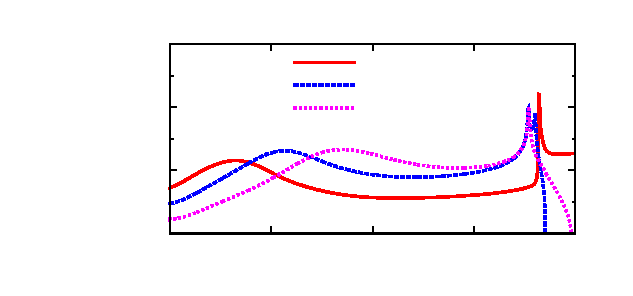
\includegraphics{1D_V_HRR}}%
    \gplfronttext
  \end{picture}%
\endgroup

  % GNUPLOT: LaTeX picture with Postscript
\begingroup
  \makeatletter
  \providecommand\color[2][]{%
    \GenericError{(gnuplot) \space\space\space\@spaces}{%
      Package color not loaded in conjunction with
      terminal option `colourtext'%
    }{See the gnuplot documentation for explanation.%
    }{Either use 'blacktext' in gnuplot or load the package
      color.sty in LaTeX.}%
    \renewcommand\color[2][]{}%
  }%
  \providecommand\includegraphics[2][]{%
    \GenericError{(gnuplot) \space\space\space\@spaces}{%
      Package graphicx or graphics not loaded%
    }{See the gnuplot documentation for explanation.%
    }{The gnuplot epslatex terminal needs graphicx.sty or graphics.sty.}%
    \renewcommand\includegraphics[2][]{}%
  }%
  \providecommand\rotatebox[2]{#2}%
  \@ifundefined{ifGPcolor}{%
    \newif\ifGPcolor
    \GPcolortrue
  }{}%
  \@ifundefined{ifGPblacktext}{%
    \newif\ifGPblacktext
    \GPblacktexttrue
  }{}%
  % define a \g@addto@macro without @ in the name:
  \let\gplgaddtomacro\g@addto@macro
  % define empty templates for all commands taking text:
  \gdef\gplbacktext{}%
  \gdef\gplfronttext{}%
  \makeatother
  \ifGPblacktext
    % no textcolor at all
    \def\colorrgb#1{}%
    \def\colorgray#1{}%
  \else
    % gray or color?
    \ifGPcolor
      \def\colorrgb#1{\color[rgb]{#1}}%
      \def\colorgray#1{\color[gray]{#1}}%
      \expandafter\def\csname LTw\endcsname{\color{white}}%
      \expandafter\def\csname LTb\endcsname{\color{black}}%
      \expandafter\def\csname LTa\endcsname{\color{black}}%
      \expandafter\def\csname LT0\endcsname{\color[rgb]{1,0,0}}%
      \expandafter\def\csname LT1\endcsname{\color[rgb]{0,1,0}}%
      \expandafter\def\csname LT2\endcsname{\color[rgb]{0,0,1}}%
      \expandafter\def\csname LT3\endcsname{\color[rgb]{1,0,1}}%
      \expandafter\def\csname LT4\endcsname{\color[rgb]{0,1,1}}%
      \expandafter\def\csname LT5\endcsname{\color[rgb]{1,1,0}}%
      \expandafter\def\csname LT6\endcsname{\color[rgb]{0,0,0}}%
      \expandafter\def\csname LT7\endcsname{\color[rgb]{1,0.3,0}}%
      \expandafter\def\csname LT8\endcsname{\color[rgb]{0.5,0.5,0.5}}%
    \else
      % gray
      \def\colorrgb#1{\color{black}}%
      \def\colorgray#1{\color[gray]{#1}}%
      \expandafter\def\csname LTw\endcsname{\color{white}}%
      \expandafter\def\csname LTb\endcsname{\color{black}}%
      \expandafter\def\csname LTa\endcsname{\color{black}}%
      \expandafter\def\csname LT0\endcsname{\color{black}}%
      \expandafter\def\csname LT1\endcsname{\color{black}}%
      \expandafter\def\csname LT2\endcsname{\color{black}}%
      \expandafter\def\csname LT3\endcsname{\color{black}}%
      \expandafter\def\csname LT4\endcsname{\color{black}}%
      \expandafter\def\csname LT5\endcsname{\color{black}}%
      \expandafter\def\csname LT6\endcsname{\color{black}}%
      \expandafter\def\csname LT7\endcsname{\color{black}}%
      \expandafter\def\csname LT8\endcsname{\color{black}}%
    \fi
  \fi
  \setlength{\unitlength}{0.0500bp}%
  \begin{picture}(5760.00,2520.00)%
    \gplgaddtomacro\gplbacktext{%
      \csname LTb\endcsname%
      \put(1342,440){\makebox(0,0)[r]{\strut{}5.0e+02}}%
      \put(1342,1045){\makebox(0,0)[r]{\strut{}1.2e+03}}%
      \put(1342,1651){\makebox(0,0)[r]{\strut{}1.9e+03}}%
      \put(1342,2256){\makebox(0,0)[r]{\strut{}2.6e+03}}%
      \put(1474,220){\makebox(0,0){\strut{} 0}}%
      \put(2446,220){\makebox(0,0){\strut{} 0.3}}%
      \put(3419,220){\makebox(0,0){\strut{} 0.6}}%
      \put(4391,220){\makebox(0,0){\strut{} 0.9}}%
      \put(5363,220){\makebox(0,0){\strut{} 1.2}}%
      \put(176,1348){\rotatebox{-270}{\makebox(0,0){\strut{}\vspace{-28pt}$T$ [K]}}}%
    }%
    \gplgaddtomacro\gplfronttext{%
      \csname LTb\endcsname%
      \put(2530,2083){\makebox(0,0)[r]{\strut{}$Z_{\rm st}$}}%
      \csname LTb\endcsname%
      \put(2530,1863){\makebox(0,0)[r]{\strut{}$Z = 0.2$}}%
      \csname LTb\endcsname%
      \put(2530,1643){\makebox(0,0)[r]{\strut{}$Z = 0.3$}}%
    }%
    \gplbacktext
    \put(0,0){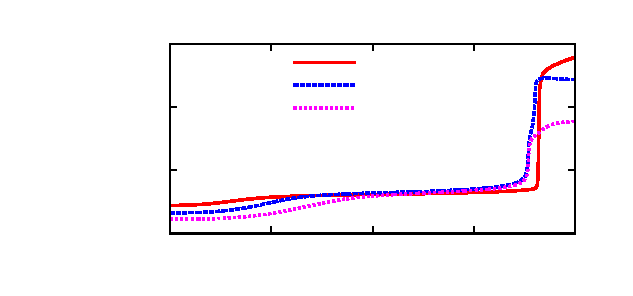
\includegraphics{ch-dynamics/1D_V_T}}%
    \gplfronttext
  \end{picture}%
\endgroup

  % GNUPLOT: LaTeX picture with Postscript
\begingroup
  \makeatletter
  \providecommand\color[2][]{%
    \GenericError{(gnuplot) \space\space\space\@spaces}{%
      Package color not loaded in conjunction with
      terminal option `colourtext'%
    }{See the gnuplot documentation for explanation.%
    }{Either use 'blacktext' in gnuplot or load the package
      color.sty in LaTeX.}%
    \renewcommand\color[2][]{}%
  }%
  \providecommand\includegraphics[2][]{%
    \GenericError{(gnuplot) \space\space\space\@spaces}{%
      Package graphicx or graphics not loaded%
    }{See the gnuplot documentation for explanation.%
    }{The gnuplot epslatex terminal needs graphicx.sty or graphics.sty.}%
    \renewcommand\includegraphics[2][]{}%
  }%
  \providecommand\rotatebox[2]{#2}%
  \@ifundefined{ifGPcolor}{%
    \newif\ifGPcolor
    \GPcolortrue
  }{}%
  \@ifundefined{ifGPblacktext}{%
    \newif\ifGPblacktext
    \GPblacktexttrue
  }{}%
  % define a \g@addto@macro without @ in the name:
  \let\gplgaddtomacro\g@addto@macro
  % define empty templates for all commands taking text:
  \gdef\gplbacktext{}%
  \gdef\gplfronttext{}%
  \makeatother
  \ifGPblacktext
    % no textcolor at all
    \def\colorrgb#1{}%
    \def\colorgray#1{}%
  \else
    % gray or color?
    \ifGPcolor
      \def\colorrgb#1{\color[rgb]{#1}}%
      \def\colorgray#1{\color[gray]{#1}}%
      \expandafter\def\csname LTw\endcsname{\color{white}}%
      \expandafter\def\csname LTb\endcsname{\color{black}}%
      \expandafter\def\csname LTa\endcsname{\color{black}}%
      \expandafter\def\csname LT0\endcsname{\color[rgb]{1,0,0}}%
      \expandafter\def\csname LT1\endcsname{\color[rgb]{0,1,0}}%
      \expandafter\def\csname LT2\endcsname{\color[rgb]{0,0,1}}%
      \expandafter\def\csname LT3\endcsname{\color[rgb]{1,0,1}}%
      \expandafter\def\csname LT4\endcsname{\color[rgb]{0,1,1}}%
      \expandafter\def\csname LT5\endcsname{\color[rgb]{1,1,0}}%
      \expandafter\def\csname LT6\endcsname{\color[rgb]{0,0,0}}%
      \expandafter\def\csname LT7\endcsname{\color[rgb]{1,0.3,0}}%
      \expandafter\def\csname LT8\endcsname{\color[rgb]{0.5,0.5,0.5}}%
    \else
      % gray
      \def\colorrgb#1{\color{black}}%
      \def\colorgray#1{\color[gray]{#1}}%
      \expandafter\def\csname LTw\endcsname{\color{white}}%
      \expandafter\def\csname LTb\endcsname{\color{black}}%
      \expandafter\def\csname LTa\endcsname{\color{black}}%
      \expandafter\def\csname LT0\endcsname{\color{black}}%
      \expandafter\def\csname LT1\endcsname{\color{black}}%
      \expandafter\def\csname LT2\endcsname{\color{black}}%
      \expandafter\def\csname LT3\endcsname{\color{black}}%
      \expandafter\def\csname LT4\endcsname{\color{black}}%
      \expandafter\def\csname LT5\endcsname{\color{black}}%
      \expandafter\def\csname LT6\endcsname{\color{black}}%
      \expandafter\def\csname LT7\endcsname{\color{black}}%
      \expandafter\def\csname LT8\endcsname{\color{black}}%
    \fi
  \fi
  \setlength{\unitlength}{0.0500bp}%
  \begin{picture}(5760.00,2520.00)%
    \gplgaddtomacro\gplbacktext{%
      \csname LTb\endcsname%
      \put(1342,440){\makebox(0,0)[r]{\strut{}1.0e-08}}%
      \put(1342,1045){\makebox(0,0)[r]{\strut{}1.0e-06}}%
      \put(1342,1651){\makebox(0,0)[r]{\strut{}1.0e-04}}%
      \put(1342,2256){\makebox(0,0)[r]{\strut{}1.0e-02}}%
      \put(1474,220){\makebox(0,0){\strut{} 0}}%
      \put(2446,220){\makebox(0,0){\strut{} 0.3}}%
      \put(3419,220){\makebox(0,0){\strut{} 0.6}}%
      \put(4391,220){\makebox(0,0){\strut{} 0.9}}%
      \put(5363,220){\makebox(0,0){\strut{} 1.2}}%
      \put(176,1348){\rotatebox{-270}{\makebox(0,0){\strut{}\vspace{-28pt}OH Mass Fraction}}}%
    }%
    \gplgaddtomacro\gplfronttext{%
      \csname LTb\endcsname%
      \put(2530,2083){\makebox(0,0)[r]{\strut{}$Z_{\rm st}$}}%
      \csname LTb\endcsname%
      \put(2530,1863){\makebox(0,0)[r]{\strut{}$Z = 0.2$}}%
      \csname LTb\endcsname%
      \put(2530,1643){\makebox(0,0)[r]{\strut{}$Z = 0.3$}}%
    }%
    \gplbacktext
    \put(0,0){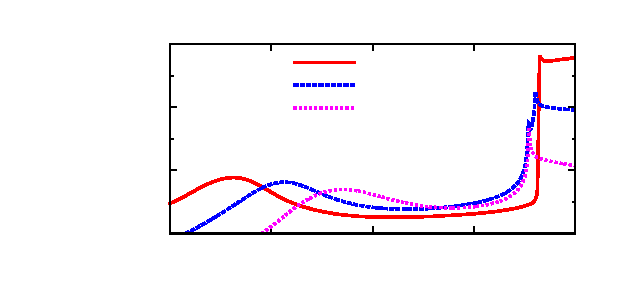
\includegraphics{1D_V_OH}}%
    \gplfronttext
  \end{picture}%
\endgroup

  % GNUPLOT: LaTeX picture with Postscript
\begingroup
  \makeatletter
  \providecommand\color[2][]{%
    \GenericError{(gnuplot) \space\space\space\@spaces}{%
      Package color not loaded in conjunction with
      terminal option `colourtext'%
    }{See the gnuplot documentation for explanation.%
    }{Either use 'blacktext' in gnuplot or load the package
      color.sty in LaTeX.}%
    \renewcommand\color[2][]{}%
  }%
  \providecommand\includegraphics[2][]{%
    \GenericError{(gnuplot) \space\space\space\@spaces}{%
      Package graphicx or graphics not loaded%
    }{See the gnuplot documentation for explanation.%
    }{The gnuplot epslatex terminal needs graphicx.sty or graphics.sty.}%
    \renewcommand\includegraphics[2][]{}%
  }%
  \providecommand\rotatebox[2]{#2}%
  \@ifundefined{ifGPcolor}{%
    \newif\ifGPcolor
    \GPcolortrue
  }{}%
  \@ifundefined{ifGPblacktext}{%
    \newif\ifGPblacktext
    \GPblacktexttrue
  }{}%
  % define a \g@addto@macro without @ in the name:
  \let\gplgaddtomacro\g@addto@macro
  % define empty templates for all commands taking text:
  \gdef\gplbacktext{}%
  \gdef\gplfronttext{}%
  \makeatother
  \ifGPblacktext
    % no textcolor at all
    \def\colorrgb#1{}%
    \def\colorgray#1{}%
  \else
    % gray or color?
    \ifGPcolor
      \def\colorrgb#1{\color[rgb]{#1}}%
      \def\colorgray#1{\color[gray]{#1}}%
      \expandafter\def\csname LTw\endcsname{\color{white}}%
      \expandafter\def\csname LTb\endcsname{\color{black}}%
      \expandafter\def\csname LTa\endcsname{\color{black}}%
      \expandafter\def\csname LT0\endcsname{\color[rgb]{1,0,0}}%
      \expandafter\def\csname LT1\endcsname{\color[rgb]{0,1,0}}%
      \expandafter\def\csname LT2\endcsname{\color[rgb]{0,0,1}}%
      \expandafter\def\csname LT3\endcsname{\color[rgb]{1,0,1}}%
      \expandafter\def\csname LT4\endcsname{\color[rgb]{0,1,1}}%
      \expandafter\def\csname LT5\endcsname{\color[rgb]{1,1,0}}%
      \expandafter\def\csname LT6\endcsname{\color[rgb]{0,0,0}}%
      \expandafter\def\csname LT7\endcsname{\color[rgb]{1,0.3,0}}%
      \expandafter\def\csname LT8\endcsname{\color[rgb]{0.5,0.5,0.5}}%
    \else
      % gray
      \def\colorrgb#1{\color{black}}%
      \def\colorgray#1{\color[gray]{#1}}%
      \expandafter\def\csname LTw\endcsname{\color{white}}%
      \expandafter\def\csname LTb\endcsname{\color{black}}%
      \expandafter\def\csname LTa\endcsname{\color{black}}%
      \expandafter\def\csname LT0\endcsname{\color{black}}%
      \expandafter\def\csname LT1\endcsname{\color{black}}%
      \expandafter\def\csname LT2\endcsname{\color{black}}%
      \expandafter\def\csname LT3\endcsname{\color{black}}%
      \expandafter\def\csname LT4\endcsname{\color{black}}%
      \expandafter\def\csname LT5\endcsname{\color{black}}%
      \expandafter\def\csname LT6\endcsname{\color{black}}%
      \expandafter\def\csname LT7\endcsname{\color{black}}%
      \expandafter\def\csname LT8\endcsname{\color{black}}%
    \fi
  \fi
  \setlength{\unitlength}{0.0500bp}%
  \begin{picture}(5760.00,2520.00)%
    \gplgaddtomacro\gplbacktext{%
      \csname LTb\endcsname%
      \put(1342,440){\makebox(0,0)[r]{\strut{}1.0e-08}}%
      \put(1342,1045){\makebox(0,0)[r]{\strut{}1.0e-06}}%
      \put(1342,1651){\makebox(0,0)[r]{\strut{}1.0e-04}}%
      \put(1342,2256){\makebox(0,0)[r]{\strut{}1.0e-02}}%
      \put(1474,220){\makebox(0,0){\strut{} 0}}%
      \put(2446,220){\makebox(0,0){\strut{} 0.3}}%
      \put(3419,220){\makebox(0,0){\strut{} 0.6}}%
      \put(4391,220){\makebox(0,0){\strut{} 0.9}}%
      \put(5363,220){\makebox(0,0){\strut{} 1.2}}%
      \put(176,1348){\rotatebox{-270}{\makebox(0,0){\strut{}\vspace{-28pt}CH$_3$OCH$_2$O$_2$ Mass Fraction}}}%
    }%
    \gplgaddtomacro\gplfronttext{%
      \csname LTb\endcsname%
      \put(2530,1053){\makebox(0,0)[r]{\strut{}$Z_{\rm st}$}}%
      \csname LTb\endcsname%
      \put(2530,833){\makebox(0,0)[r]{\strut{}$Z = 0.2$}}%
      \csname LTb\endcsname%
      \put(2530,613){\makebox(0,0)[r]{\strut{}$Z = 0.3$}}%
    }%
    \gplbacktext
    \put(0,0){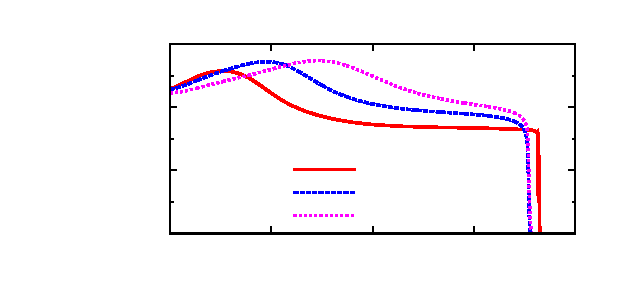
\includegraphics{1D_V_RO2}}%
    \gplfronttext
  \end{picture}%
\endgroup

  % GNUPLOT: LaTeX picture with Postscript
\begingroup
  \makeatletter
  \providecommand\color[2][]{%
    \GenericError{(gnuplot) \space\space\space\@spaces}{%
      Package color not loaded in conjunction with
      terminal option `colourtext'%
    }{See the gnuplot documentation for explanation.%
    }{Either use 'blacktext' in gnuplot or load the package
      color.sty in LaTeX.}%
    \renewcommand\color[2][]{}%
  }%
  \providecommand\includegraphics[2][]{%
    \GenericError{(gnuplot) \space\space\space\@spaces}{%
      Package graphicx or graphics not loaded%
    }{See the gnuplot documentation for explanation.%
    }{The gnuplot epslatex terminal needs graphicx.sty or graphics.sty.}%
    \renewcommand\includegraphics[2][]{}%
  }%
  \providecommand\rotatebox[2]{#2}%
  \@ifundefined{ifGPcolor}{%
    \newif\ifGPcolor
    \GPcolortrue
  }{}%
  \@ifundefined{ifGPblacktext}{%
    \newif\ifGPblacktext
    \GPblacktexttrue
  }{}%
  % define a \g@addto@macro without @ in the name:
  \let\gplgaddtomacro\g@addto@macro
  % define empty templates for all commands taking text:
  \gdef\gplbacktext{}%
  \gdef\gplfronttext{}%
  \makeatother
  \ifGPblacktext
    % no textcolor at all
    \def\colorrgb#1{}%
    \def\colorgray#1{}%
  \else
    % gray or color?
    \ifGPcolor
      \def\colorrgb#1{\color[rgb]{#1}}%
      \def\colorgray#1{\color[gray]{#1}}%
      \expandafter\def\csname LTw\endcsname{\color{white}}%
      \expandafter\def\csname LTb\endcsname{\color{black}}%
      \expandafter\def\csname LTa\endcsname{\color{black}}%
      \expandafter\def\csname LT0\endcsname{\color[rgb]{1,0,0}}%
      \expandafter\def\csname LT1\endcsname{\color[rgb]{0,1,0}}%
      \expandafter\def\csname LT2\endcsname{\color[rgb]{0,0,1}}%
      \expandafter\def\csname LT3\endcsname{\color[rgb]{1,0,1}}%
      \expandafter\def\csname LT4\endcsname{\color[rgb]{0,1,1}}%
      \expandafter\def\csname LT5\endcsname{\color[rgb]{1,1,0}}%
      \expandafter\def\csname LT6\endcsname{\color[rgb]{0,0,0}}%
      \expandafter\def\csname LT7\endcsname{\color[rgb]{1,0.3,0}}%
      \expandafter\def\csname LT8\endcsname{\color[rgb]{0.5,0.5,0.5}}%
    \else
      % gray
      \def\colorrgb#1{\color{black}}%
      \def\colorgray#1{\color[gray]{#1}}%
      \expandafter\def\csname LTw\endcsname{\color{white}}%
      \expandafter\def\csname LTb\endcsname{\color{black}}%
      \expandafter\def\csname LTa\endcsname{\color{black}}%
      \expandafter\def\csname LT0\endcsname{\color{black}}%
      \expandafter\def\csname LT1\endcsname{\color{black}}%
      \expandafter\def\csname LT2\endcsname{\color{black}}%
      \expandafter\def\csname LT3\endcsname{\color{black}}%
      \expandafter\def\csname LT4\endcsname{\color{black}}%
      \expandafter\def\csname LT5\endcsname{\color{black}}%
      \expandafter\def\csname LT6\endcsname{\color{black}}%
      \expandafter\def\csname LT7\endcsname{\color{black}}%
      \expandafter\def\csname LT8\endcsname{\color{black}}%
    \fi
  \fi
  \setlength{\unitlength}{0.0500bp}%
  \begin{picture}(5760.00,2520.00)%
    \gplgaddtomacro\gplbacktext{%
      \csname LTb\endcsname%
      \put(1342,704){\makebox(0,0)[r]{\strut{}1.0e-07}}%
      \put(1342,1221){\makebox(0,0)[r]{\strut{}1.0e-05}}%
      \put(1342,1739){\makebox(0,0)[r]{\strut{}1.0e-03}}%
      \put(1342,2256){\makebox(0,0)[r]{\strut{}1.0e-01}}%
      \put(1474,484){\makebox(0,0){\strut{} 0}}%
      \put(2446,484){\makebox(0,0){\strut{} 0.3}}%
      \put(3419,484){\makebox(0,0){\strut{} 0.6}}%
      \put(4391,484){\makebox(0,0){\strut{} 0.9}}%
      \put(5363,484){\makebox(0,0){\strut{} 1.2}}%
      \put(176,1480){\rotatebox{-270}{\makebox(0,0){\strut{}\vspace{-28pt}H$_2$O$_2$ Mass Fraction}}}%
      \put(3418,154){\makebox(0,0){\strut{}Time [ms]}}%
    }%
    \gplgaddtomacro\gplfronttext{%
      \csname LTb\endcsname%
      \put(2530,1317){\makebox(0,0)[r]{\strut{}$Z_{\rm st}$}}%
      \csname LTb\endcsname%
      \put(2530,1097){\makebox(0,0)[r]{\strut{}$Z = 0.2$}}%
      \csname LTb\endcsname%
      \put(2530,877){\makebox(0,0)[r]{\strut{}$Z = 0.3$}}%
    }%
    \gplbacktext
    \put(0,0){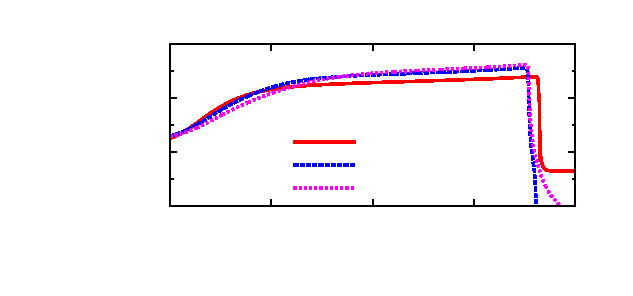
\includegraphics{1D_V_H2O2}}%
    \gplfronttext
  \end{picture}%
\endgroup

  \normalsize
  \caption{LFA profiles along $Z_{\rm st}$, $Z = 0.2$, and $Z = 0.3$ of the $8.0$ m/s case.}
  \label{fig:1D_V}
\end{figure}

The multibrachial structure of the inhomogeneous autoignition front is due to the variation in ignition delay time at different mixture fractions.  As shown in Fig.~\ref{fig:HRR_V}, the stabilization point is determined based on the threshold value of heat release rate.  Therefore, the ignition delay time of inhomogeneous autoignition can be determined accordingly, which corresponds to the heat release rate peak that exceeds $10^{12}$ J/m$^3$-s.  For the $8.0$ m/s case shown in Fig.~\ref{fig:tau}, the mixture is autoignited first at $Z = 0.24$, which corresponds to the stabilization point in Fig.~\ref{fig:HRR_V}.  Although the first stage ignition delay time, defined by the first heat release peak through low-temperature chemistry, increases monotonically as mixture fraction increases (temperature decreases), the overall ignition delay time reaches the shortest at $Z = 0.24$ due to the compensation of larger heat release after the first ignition stage~\cite{law12}, as shown in Fig.~\ref{fig:1D_V}.  As a consequence, although low-temperature chemistry is not the dominant chemical pathway at the stabilization point for the \emph{kinetically} stabilized case, it still influences the location of the stabilization point through the mixture fraction dependent heat and radical accumulation upstream.   

\begin{figure}
  \centering
  \scriptsize
  \resizebox{0.6\textwidth}{!}{% GNUPLOT: LaTeX picture with Postscript
\begingroup
  \makeatletter
  \providecommand\color[2][]{%
    \GenericError{(gnuplot) \space\space\space\@spaces}{%
      Package color not loaded in conjunction with
      terminal option `colourtext'%
    }{See the gnuplot documentation for explanation.%
    }{Either use 'blacktext' in gnuplot or load the package
      color.sty in LaTeX.}%
    \renewcommand\color[2][]{}%
  }%
  \providecommand\includegraphics[2][]{%
    \GenericError{(gnuplot) \space\space\space\@spaces}{%
      Package graphicx or graphics not loaded%
    }{See the gnuplot documentation for explanation.%
    }{The gnuplot epslatex terminal needs graphicx.sty or graphics.sty.}%
    \renewcommand\includegraphics[2][]{}%
  }%
  \providecommand\rotatebox[2]{#2}%
  \@ifundefined{ifGPcolor}{%
    \newif\ifGPcolor
    \GPcolortrue
  }{}%
  \@ifundefined{ifGPblacktext}{%
    \newif\ifGPblacktext
    \GPblacktexttrue
  }{}%
  % define a \g@addto@macro without @ in the name:
  \let\gplgaddtomacro\g@addto@macro
  % define empty templates for all commands taking text:
  \gdef\gplbacktext{}%
  \gdef\gplfronttext{}%
  \makeatother
  \ifGPblacktext
    % no textcolor at all
    \def\colorrgb#1{}%
    \def\colorgray#1{}%
  \else
    % gray or color?
    \ifGPcolor
      \def\colorrgb#1{\color[rgb]{#1}}%
      \def\colorgray#1{\color[gray]{#1}}%
      \expandafter\def\csname LTw\endcsname{\color{white}}%
      \expandafter\def\csname LTb\endcsname{\color{black}}%
      \expandafter\def\csname LTa\endcsname{\color{black}}%
      \expandafter\def\csname LT0\endcsname{\color[rgb]{1,0,0}}%
      \expandafter\def\csname LT1\endcsname{\color[rgb]{0,1,0}}%
      \expandafter\def\csname LT2\endcsname{\color[rgb]{0,0,1}}%
      \expandafter\def\csname LT3\endcsname{\color[rgb]{1,0,1}}%
      \expandafter\def\csname LT4\endcsname{\color[rgb]{0,1,1}}%
      \expandafter\def\csname LT5\endcsname{\color[rgb]{1,1,0}}%
      \expandafter\def\csname LT6\endcsname{\color[rgb]{0,0,0}}%
      \expandafter\def\csname LT7\endcsname{\color[rgb]{1,0.3,0}}%
      \expandafter\def\csname LT8\endcsname{\color[rgb]{0.5,0.5,0.5}}%
    \else
      % gray
      \def\colorrgb#1{\color{black}}%
      \def\colorgray#1{\color[gray]{#1}}%
      \expandafter\def\csname LTw\endcsname{\color{white}}%
      \expandafter\def\csname LTb\endcsname{\color{black}}%
      \expandafter\def\csname LTa\endcsname{\color{black}}%
      \expandafter\def\csname LT0\endcsname{\color{black}}%
      \expandafter\def\csname LT1\endcsname{\color{black}}%
      \expandafter\def\csname LT2\endcsname{\color{black}}%
      \expandafter\def\csname LT3\endcsname{\color{black}}%
      \expandafter\def\csname LT4\endcsname{\color{black}}%
      \expandafter\def\csname LT5\endcsname{\color{black}}%
      \expandafter\def\csname LT6\endcsname{\color{black}}%
      \expandafter\def\csname LT7\endcsname{\color{black}}%
      \expandafter\def\csname LT8\endcsname{\color{black}}%
    \fi
  \fi
  \setlength{\unitlength}{0.0500bp}%
  \begin{picture}(3600.00,2520.00)%
    \gplgaddtomacro\gplbacktext{%
      \csname LTb\endcsname%
      \put(1078,704){\makebox(0,0)[r]{\strut{} 1.05}}%
      \put(1078,1221){\makebox(0,0)[r]{\strut{} 1.07}}%
      \put(1078,1739){\makebox(0,0)[r]{\strut{} 1.09}}%
      \put(1078,2256){\makebox(0,0)[r]{\strut{} 1.11}}%
      \put(1210,484){\makebox(0,0){\strut{} 0}}%
      \put(1708,484){\makebox(0,0){\strut{} 0.1}}%
      \put(2207,484){\makebox(0,0){\strut{} 0.2}}%
      \put(2705,484){\makebox(0,0){\strut{} 0.3}}%
      \put(3203,484){\makebox(0,0){\strut{} 0.4}}%
      \put(176,1480){\rotatebox{-270}{\makebox(0,0){\strut{}\vspace{-28pt}Iginition Delay [ms]}}}%
      \put(2206,154){\makebox(0,0){\strut{}Z}}%
    }%
    \gplgaddtomacro\gplfronttext{%
    }%
    \gplbacktext
    \put(0,0){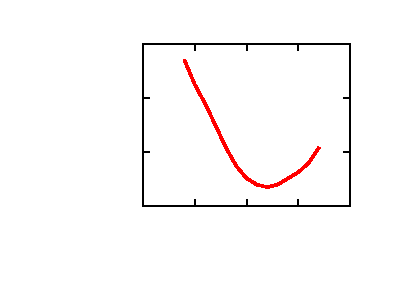
\includegraphics{tau_t}}%
    \gplfronttext
  \end{picture}%
\endgroup
}
  \resizebox{0.6\textwidth}{!}{% GNUPLOT: LaTeX picture with Postscript
\begingroup
  \makeatletter
  \providecommand\color[2][]{%
    \GenericError{(gnuplot) \space\space\space\@spaces}{%
      Package color not loaded in conjunction with
      terminal option `colourtext'%
    }{See the gnuplot documentation for explanation.%
    }{Either use 'blacktext' in gnuplot or load the package
      color.sty in LaTeX.}%
    \renewcommand\color[2][]{}%
  }%
  \providecommand\includegraphics[2][]{%
    \GenericError{(gnuplot) \space\space\space\@spaces}{%
      Package graphicx or graphics not loaded%
    }{See the gnuplot documentation for explanation.%
    }{The gnuplot epslatex terminal needs graphicx.sty or graphics.sty.}%
    \renewcommand\includegraphics[2][]{}%
  }%
  \providecommand\rotatebox[2]{#2}%
  \@ifundefined{ifGPcolor}{%
    \newif\ifGPcolor
    \GPcolortrue
  }{}%
  \@ifundefined{ifGPblacktext}{%
    \newif\ifGPblacktext
    \GPblacktexttrue
  }{}%
  % define a \g@addto@macro without @ in the name:
  \let\gplgaddtomacro\g@addto@macro
  % define empty templates for all commands taking text:
  \gdef\gplbacktext{}%
  \gdef\gplfronttext{}%
  \makeatother
  \ifGPblacktext
    % no textcolor at all
    \def\colorrgb#1{}%
    \def\colorgray#1{}%
  \else
    % gray or color?
    \ifGPcolor
      \def\colorrgb#1{\color[rgb]{#1}}%
      \def\colorgray#1{\color[gray]{#1}}%
      \expandafter\def\csname LTw\endcsname{\color{white}}%
      \expandafter\def\csname LTb\endcsname{\color{black}}%
      \expandafter\def\csname LTa\endcsname{\color{black}}%
      \expandafter\def\csname LT0\endcsname{\color[rgb]{1,0,0}}%
      \expandafter\def\csname LT1\endcsname{\color[rgb]{0,1,0}}%
      \expandafter\def\csname LT2\endcsname{\color[rgb]{0,0,1}}%
      \expandafter\def\csname LT3\endcsname{\color[rgb]{1,0,1}}%
      \expandafter\def\csname LT4\endcsname{\color[rgb]{0,1,1}}%
      \expandafter\def\csname LT5\endcsname{\color[rgb]{1,1,0}}%
      \expandafter\def\csname LT6\endcsname{\color[rgb]{0,0,0}}%
      \expandafter\def\csname LT7\endcsname{\color[rgb]{1,0.3,0}}%
      \expandafter\def\csname LT8\endcsname{\color[rgb]{0.5,0.5,0.5}}%
    \else
      % gray
      \def\colorrgb#1{\color{black}}%
      \def\colorgray#1{\color[gray]{#1}}%
      \expandafter\def\csname LTw\endcsname{\color{white}}%
      \expandafter\def\csname LTb\endcsname{\color{black}}%
      \expandafter\def\csname LTa\endcsname{\color{black}}%
      \expandafter\def\csname LT0\endcsname{\color{black}}%
      \expandafter\def\csname LT1\endcsname{\color{black}}%
      \expandafter\def\csname LT2\endcsname{\color{black}}%
      \expandafter\def\csname LT3\endcsname{\color{black}}%
      \expandafter\def\csname LT4\endcsname{\color{black}}%
      \expandafter\def\csname LT5\endcsname{\color{black}}%
      \expandafter\def\csname LT6\endcsname{\color{black}}%
      \expandafter\def\csname LT7\endcsname{\color{black}}%
      \expandafter\def\csname LT8\endcsname{\color{black}}%
    \fi
  \fi
  \setlength{\unitlength}{0.0500bp}%
  \begin{picture}(3528.00,2520.00)%
    \gplgaddtomacro\gplbacktext{%
      \csname LTb\endcsname%
      \put(946,704){\makebox(0,0)[r]{\strut{} 0}}%
      \put(946,1221){\makebox(0,0)[r]{\strut{} 0.3}}%
      \put(946,1739){\makebox(0,0)[r]{\strut{} 0.6}}%
      \put(946,2256){\makebox(0,0)[r]{\strut{} 0.9}}%
      \put(1078,484){\makebox(0,0){\strut{} 0}}%
      \put(1591,484){\makebox(0,0){\strut{} 0.1}}%
      \put(2105,484){\makebox(0,0){\strut{} 0.2}}%
      \put(2618,484){\makebox(0,0){\strut{} 0.3}}%
      \put(3131,484){\makebox(0,0){\strut{} 0.4}}%
      \put(176,1480){\rotatebox{-270}{\makebox(0,0){\strut{}\vspace{-28pt}First Stage Ignition Delay [ms]}}}%
      \put(2104,154){\makebox(0,0){\strut{}Z}}%
    }%
    \gplgaddtomacro\gplfronttext{%
    }%
    \gplbacktext
    \put(0,0){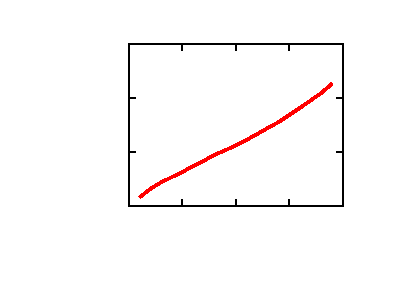
\includegraphics{ch-dynamics/tau_1}}%
    \gplfronttext
  \end{picture}%
\endgroup
}
  \normalsize
  \caption{LFA results on the mixture fraction dependent total and first stage ignition delay times of the $8.0$ m/s case.}
  \label{fig:tau}
\end{figure}          

However, although the cases discussed are all initiated by inhomogeneous autoignition, the stabilization of the final structure depends on the dominant transport processes, which are influenced by the inlet velocities.  At $8.0$ m/s, heat and radical back diffusion from the autoignition front to upstream is not able to keep up with convection; therefore, the reacting front is \emph{kinetically} stabilized.  At $3.2$ m/s, as flow convection is weaker, diffusion processes become inherently important and couple with chemical reactions to induce a flame front propagating upstream.  However, the propagation speed of the flame varies with composition and temperature.  As a consequence, around $Z_{\rm st}$, where higher temperature and near-stoichiometric mixture composition enable higher local flame speed, the propagation of the reacting front balances the incoming flow velocity.  However, such a balance fails at richer mixture fractions where \emph{kinetic} stabilization dominates due to enhanced NTC-affected autoignition at richer mixture fractions as demonstrated in Fig.~\ref{fig:tau}.  At $2.4$ m/s, back diffusion is important at all mixture fractions such that the reacting front propagates upstream at the local flame speed, as determined by the local composition and temperature.  Due to the increased temperature and species stratification and the reduced thermal and radical accumulation from autoignition, the propagation speed of this reacting front is less influenced by inhomogeneous autoignition, as demonstrated with CEMA and LFA.  The structure of this \emph{kinematically} stabilized reacting front, which is generally tribrachial, is therefore determined by the variation of the local flame speed. 

\subsection{Stabilization Regime Diagram}

The above sections have demonstrated the transport effects on the thermal and chemical structure of the lifted coflow flames as well as the stabilization mechanisms.  Combining these results with the chemical effects demonstrated by changing the coflow boundary temperature in Sec.~\ref{sec:dynamics-T}, a two-dimensional stabilization regime diagram is proposed, as shown in Fig.~\ref{fig:2D-regime}.  

\begin{figure}
  \centering
  \scriptsize
  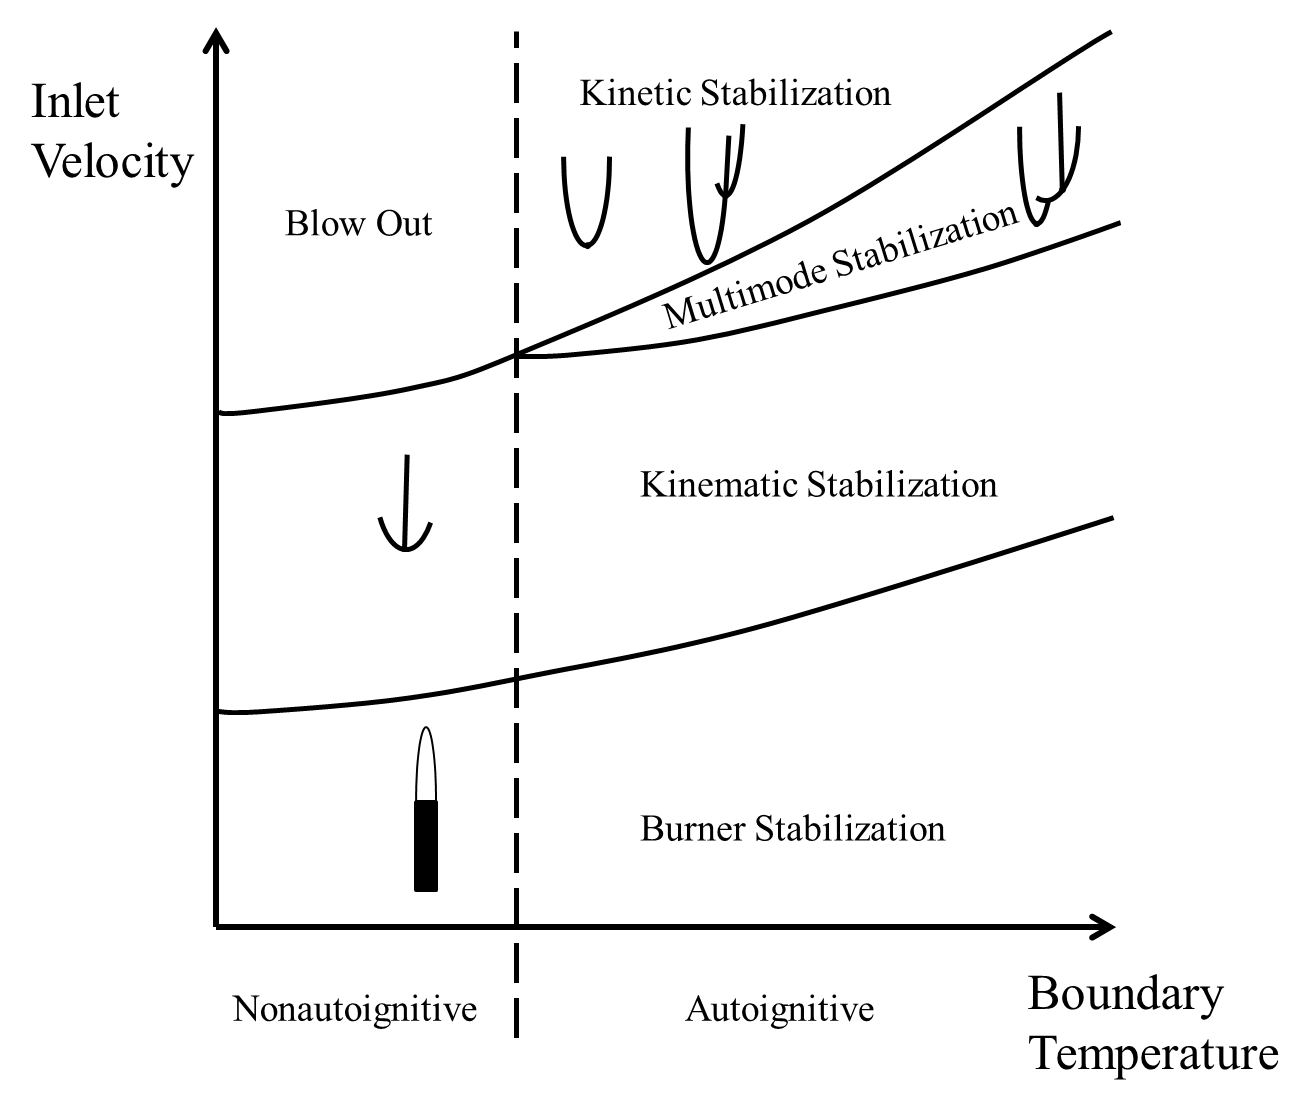
\includegraphics[width=0.8\textwidth]{ch-dynamics/2D-regime.png}
  \normalsize
  \caption{A qualitative regime diagram for the stabilization mechanisms as the boundary temperature and inlet velocity vary. }
  \label{fig:2D-regime}
\end{figure}

Qualitatively, when the boundary temperature is not high enough to activate autoignition, the lifted flame appears as the classical triple flame and is \emph{kinematically} stabilized.  When the inlet velocity is below or above certain threshold values, the triple flame becomes attached to the burner or is blown out, respectively.  

As the boundary temperature is elevated enough to activate autoignition, increasing the inlet velocity while keeping constant boundary temperature, the flame stabilization mechanism transits from burner stabilization to a \emph{kinematic} balance between flame speed and incoming flow velocity, then to multimode stabilization influenced by both flame propagation and inhomogeneous autoignition, and finally to \emph {kinetic} stabilization governed by inhomogeneous autoignition.  It is expected that the crossover velocities between regimes increase with increasing boundary temperature because flame speed generally increases at higher temperature.  However, it is difficult to quantify these boundaries as local composition and temperature vary in the streamwise direction, and, therefore, the reference flame speed cannot be calculated based on the upstream boundary conditions.  Furthermore, local flame front curvature, cross-stream species stratification, and flow divergence approaching the flame front also modify the flame speed.  As a consequence, only a qualitative trend is demonstrated in Fig.~\ref{fig:2D-regime}.  

Similarly, if the boundary temperature increases at fixed inlet velocity, transition from blow out to burner stabilized regimes is achieved by moving horizontally across the regime diagram, which was discussed in Sec.~\ref{sec:dynamics-T}.     

%---------------------------------------------

\section{Flame Dynamics in Oscillating Flows}

In this section, unsteady nonpremixed DME/air coflow flames under autoignitive conditions are computationally studied to elucidate the coupling between unsteady fluid dynamics and chemical kinetics.  Various oscillation frequencies were imposed on the inlet velocity, with the maximum and minimum velocities maintained the same as those in Sec.~\ref{sec:dynamics-V}, which correspond to an autoignition front and a tribrachial flame, respectively.  Low frequency oscillation ranging from 25 to 100 Hz, which covers buoyancy-driven instability frequencies~\cite{mohammed98,dworkin07} and acoustic-driven oscillation frequencies in gas turbines~\cite{temme12} is considered.  As the steady cases correspond to different combustion modes, it is expected that, at certain frequencies of velocity oscillation, the dominant combustion process will shift between the nonpremixed tribrachial flame mode and the autoignition mode.  Therefore, the transition in combustion mode is first presented.  The thermal and chemical differences during such transition and the transition mechanism are then discussed.  Finally, the effects of oscillation frequency on the coupling of fluid dynamics and chemical kinetics is elucidated.  The understanding of the coupling effects of chemistry and transport obtained lays the foundation for future turbulent studies.

\subsection{Thermal Structure}

As the largest and smallest inlet velocity cases were designed to match the two extreme cases in Sec.~\ref{sec:dynamics-V}, which are of different thermal structures, it is expected that similar thermal structures will be obtained.  Furthermore, these thermal structures might transition back and forth in response to the oscillating flow field.  Indeed, such transitions were observed for all three frequencies.  For example, the evolution of the thermal structure of the $100$ Hz case, in terms of the heat release rate profile, is demonstrated in Fig.~\ref{fig:HRR_100Hz}.  The oscillation cycle starts with the largest inlet velocity of $8.0$ m/s, and the minimum inlet velocity ($2.4$ m/s) is achieved at half cycle.  

\begin{figure}[t]
  \centering
  \scriptsize
  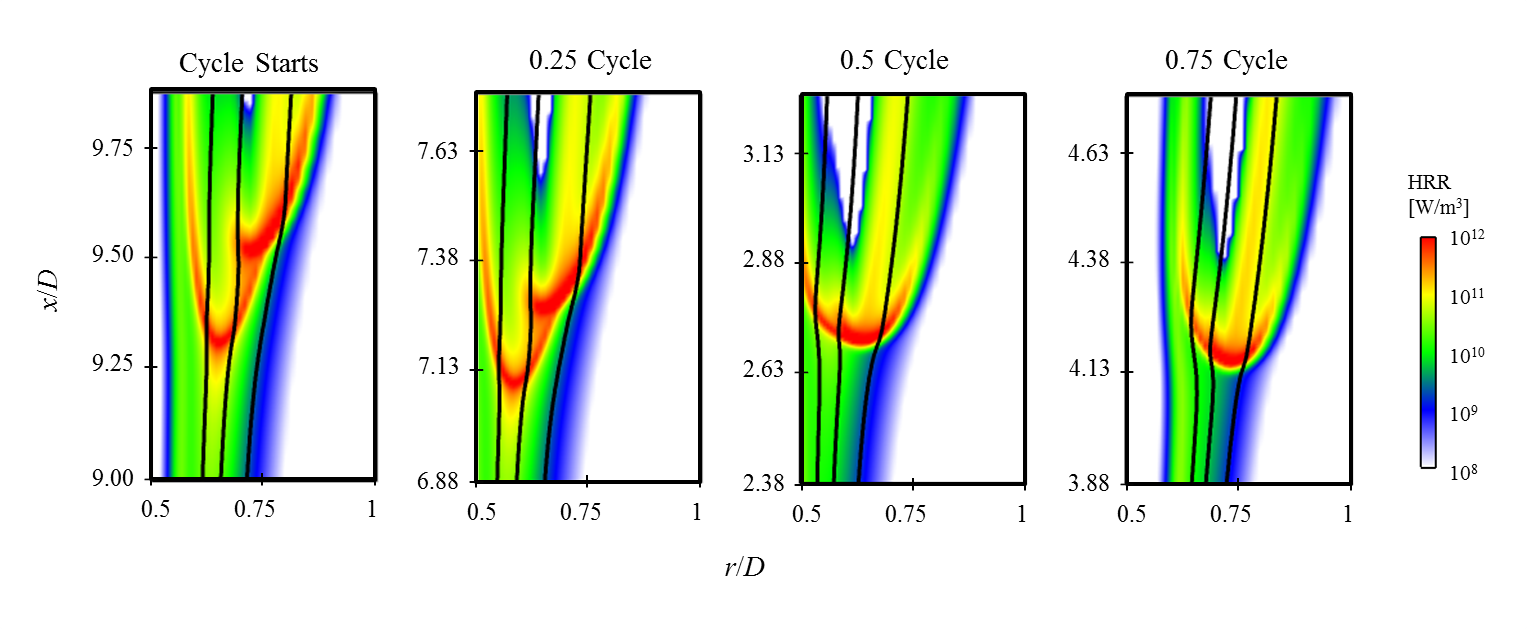
\includegraphics[trim=6.5mm 7.5mm 7mm 8mm, clip=true, width=1.0\textwidth]{ch-dynamics/HRR_100Hz.png}
  \normalsize
  \caption{Heat release rate [W/m$^3$] profile evolution during one oscillation cycle at $100$ Hz.  The iso-contours of $Z_{\rm st} = 0.1$, $Z = 0.2$, and $Z = 0.3$ are outlined from right to left in solid lines, respectively.}
  \label{fig:HRR_100Hz}
\end{figure}

At $8.0$ m/s, the multibrachial thermal structure is located furthest downstream.  The leading point, which is defined as the most upstream point that has the heat release rate value of $10^{12}$ W/m$^3$, is located at mixture fraction $Z = 0.24$.  As the inlet velocity decreases, the multibrachial structure moves upstream, without obvious change of the leading point location, in terms of mixture fraction.  When the inlet velocity reaches its minimum, the multibrachial structure transitions to a tribrachial structure, and the leading point switches to $Z = 0.14$.  As the flow velocity increases, the tribrachial structure is pushed downstream, and both its tribrachial shape and its leading point mixture fraction remain unchanged.  The thermal structure returns to that of multibrachial when the flow velocity further increases.  Such transitions in structure repeat once a new oscillation cycle starts.

\subsection{Differentiation of Combustion Mode}

In Sec.~\ref{sec:dynamics-V} the morphology of the thermal structures are related to two different combustion modes: tribrachial flame and autoignition.  Specifically, at steady state, the multibrachial structure in the $8.0$ m/s case is an autoignition front, while the $2.4$ m/s case is a tribrachial flame.  In the previouly presented steady cases, species mass fraction profiles at the inlet of the two-dimensional computation are treated as the initial conditions for one-dimensional Lagrangian Flamelet Analysis~\cite{pitsch98a}, which only considers diffusion processes parallel to the mixture fraction gradient and neglects those in the normal direction.  When the LFA prediction agrees with the CFD result, transport in the normal direction of the mixture fraction gradient is negligible, and autoignition is the dominant combustion process.  However, due to the unsteadiness in the oscillating cases, such comparison between LFA and CFD is no longer applicable, and a new criterion to differentiate the modes of tribrachial flame and autoignition needs to be identified and validated against the steady cases.

A density-weighted displacement speed, $S_d$, is often used to distinguish between deflagrations and spontaneous ignition fronts in HCCI combustion~\cite{yoo13}, which is defined from an iso-line of species $k$ as~\cite{ruetsch95,im99}:

\begin{equation} \label{eq:sd}
S_d = \frac{1}{\rho{_u} |\nabla Y_k|} \left(\dot{\omega}{_k} - \pp{\rho Y_k V_{j,k}}{x_j} \right),
\end{equation}
where $Y_k$, $V_{j,k}$, and $\dot{\omega}{_k}$ denote species mass fraction, diffusion velocity in the $j$-direction, and net production rate, respectively, and $\rho {_u}$ is the density of the unburnt mixture.  The choice of species $k$ and its iso-line value can be ambiguous.  Therefore, major products, such as CO$_2$, H$_2$O, H$_2$, CO, and combinations of these products have been tested, and the sampling location is chosen as the leading point, as defined above, to enable further comparison with the steady cases.  $S_d$ at the leading point is insensitive to the choice of species, for less than $5$\% difference was observed across all the combinations.  Consequently, H$_2$O was chosen for simplicity.  Both the laminar flame speed $S_L$ and the unburnt mixture density $\rho {_u}$ were obtained from laminar flame speed calculations using the FlameMaster code~\cite{flamemaster}.  The composition and temperature boundary conditions for the laminar flame speed calculations were based on the sampled mixture fraction at the leading point and linearly interpolated, in the mixture fraction space, between the corresponding inlet values of the fuel and coflow streams.  

Following the above procedure, displacement velocities were calculated for all three oscillation frequency cases, with $20$ points per cycle, to demonstrate their evolution.  Furthermore, as shown in Fig.~\ref{fig:sd_evo}, $S_d/S_L$ for the two steady cases ($2.4$ and $8.0$ m/s) were similarly calculated to validate this definition of normalized displacement velocity and differentiate between tribrachial flame and autoignition.  For clarity, only the 100 Hz case is included in Fig.~\ref{fig:sd_evo} to elucidate its evolution, and the effect of the oscillation frequency will be discussed in Sec.\ref{sec:frq}.

\begin{figure}[t]
  \centering
  \scriptsize
  \resizebox{1.0\textwidth}{!}{% GNUPLOT: LaTeX picture with Postscript
\begingroup
  \makeatletter
  \providecommand\color[2][]{%
    \GenericError{(gnuplot) \space\space\space\@spaces}{%
      Package color not loaded in conjunction with
      terminal option `colourtext'%
    }{See the gnuplot documentation for explanation.%
    }{Either use 'blacktext' in gnuplot or load the package
      color.sty in LaTeX.}%
    \renewcommand\color[2][]{}%
  }%
  \providecommand\includegraphics[2][]{%
    \GenericError{(gnuplot) \space\space\space\@spaces}{%
      Package graphicx or graphics not loaded%
    }{See the gnuplot documentation for explanation.%
    }{The gnuplot epslatex terminal needs graphicx.sty or graphics.sty.}%
    \renewcommand\includegraphics[2][]{}%
  }%
  \providecommand\rotatebox[2]{#2}%
  \@ifundefined{ifGPcolor}{%
    \newif\ifGPcolor
    \GPcolortrue
  }{}%
  \@ifundefined{ifGPblacktext}{%
    \newif\ifGPblacktext
    \GPblacktexttrue
  }{}%
  % define a \g@addto@macro without @ in the name:
  \let\gplgaddtomacro\g@addto@macro
  % define empty templates for all commands taking text:
  \gdef\gplbacktext{}%
  \gdef\gplfronttext{}%
  \makeatother
  \ifGPblacktext
    % no textcolor at all
    \def\colorrgb#1{}%
    \def\colorgray#1{}%
  \else
    % gray or color?
    \ifGPcolor
      \def\colorrgb#1{\color[rgb]{#1}}%
      \def\colorgray#1{\color[gray]{#1}}%
      \expandafter\def\csname LTw\endcsname{\color{white}}%
      \expandafter\def\csname LTb\endcsname{\color{black}}%
      \expandafter\def\csname LTa\endcsname{\color{black}}%
      \expandafter\def\csname LT0\endcsname{\color[rgb]{1,0,0}}%
      \expandafter\def\csname LT1\endcsname{\color[rgb]{0,1,0}}%
      \expandafter\def\csname LT2\endcsname{\color[rgb]{0,0,1}}%
      \expandafter\def\csname LT3\endcsname{\color[rgb]{1,0,1}}%
      \expandafter\def\csname LT4\endcsname{\color[rgb]{0,1,1}}%
      \expandafter\def\csname LT5\endcsname{\color[rgb]{1,1,0}}%
      \expandafter\def\csname LT6\endcsname{\color[rgb]{0,0,0}}%
      \expandafter\def\csname LT7\endcsname{\color[rgb]{1,0.3,0}}%
      \expandafter\def\csname LT8\endcsname{\color[rgb]{0.5,0.5,0.5}}%
    \else
      % gray
      \def\colorrgb#1{\color{black}}%
      \def\colorgray#1{\color[gray]{#1}}%
      \expandafter\def\csname LTw\endcsname{\color{white}}%
      \expandafter\def\csname LTb\endcsname{\color{black}}%
      \expandafter\def\csname LTa\endcsname{\color{black}}%
      \expandafter\def\csname LT0\endcsname{\color{black}}%
      \expandafter\def\csname LT1\endcsname{\color{black}}%
      \expandafter\def\csname LT2\endcsname{\color{black}}%
      \expandafter\def\csname LT3\endcsname{\color{black}}%
      \expandafter\def\csname LT4\endcsname{\color{black}}%
      \expandafter\def\csname LT5\endcsname{\color{black}}%
      \expandafter\def\csname LT6\endcsname{\color{black}}%
      \expandafter\def\csname LT7\endcsname{\color{black}}%
      \expandafter\def\csname LT8\endcsname{\color{black}}%
    \fi
  \fi
  \setlength{\unitlength}{0.0500bp}%
  \begin{picture}(5760.00,4032.00)%
    \gplgaddtomacro\gplbacktext{%
      \csname LTb\endcsname%
      \put(588,704){\makebox(0,0)[r]{\strut{} 0}}%
      \put(588,1317){\makebox(0,0)[r]{\strut{} 2}}%
      \put(588,1929){\makebox(0,0)[r]{\strut{} 4}}%
      \put(588,2542){\makebox(0,0)[r]{\strut{} 6}}%
      \put(588,3154){\makebox(0,0)[r]{\strut{} 8}}%
      \put(588,3767){\makebox(0,0)[r]{\strut{} 10}}%
      \put(720,484){\makebox(0,0){\strut{} 0}}%
      \put(1260,484){\makebox(0,0){\strut{} 0.25}}%
      \put(1800,484){\makebox(0,0){\strut{} 0.5}}%
      \put(2340,484){\makebox(0,0){\strut{} 0.75}}%
      \put(2880,484){\makebox(0,0){\strut{} 1}}%
      \put(3419,484){\makebox(0,0){\strut{} 1.25}}%
      \put(3959,484){\makebox(0,0){\strut{} 1.5}}%
      \put(4499,484){\makebox(0,0){\strut{} 1.75}}%
      \put(5039,484){\makebox(0,0){\strut{} 2}}%
      \put(5171,704){\makebox(0,0)[l]{\strut{} 0}}%
      \put(5171,1317){\makebox(0,0)[l]{\strut{} 3}}%
      \put(5171,1929){\makebox(0,0)[l]{\strut{} 6}}%
      \put(5171,2542){\makebox(0,0)[l]{\strut{} 9}}%
      \put(5171,3154){\makebox(0,0)[l]{\strut{} 12}}%
      \put(5171,3767){\makebox(0,0)[l]{\strut{} 15}}%
      \put(-50,2235){\rotatebox{-270}{\makebox(0,0){\strut{}\vspace{-28pt}$S_d/S_L$}}}%
      \put(5808,2235){\rotatebox{-270}{\makebox(0,0){\strut{}\vspace{28pt}$x_d/D$}}}%
      \put(2879,154){\makebox(0,0){\strut{}Cycle}}%
    }%
    \gplgaddtomacro\gplfronttext{%
      \csname LTb\endcsname%
      \put(2068,3679){\makebox(0,0)[r]{\strut{}Steady $S_d/S_L$}}%
      \csname LTb\endcsname%
      \put(2068,3503){\makebox(0,0)[r]{\strut{}$S_d/S_L$}}%
      \csname LTb\endcsname%
      \put(2068,3327){\makebox(0,0)[r]{\strut{}$x_d/D$}}%
    }%
    \gplbacktext
    \put(0,0){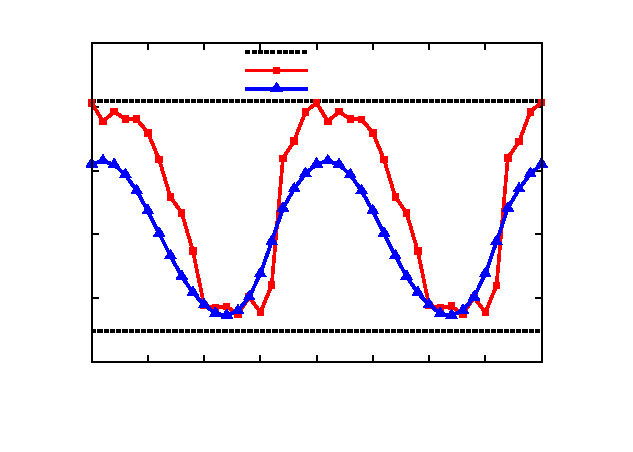
\includegraphics{sd_evo}}%
    \gplfronttext
  \end{picture}%
\endgroup
}
  \normalsize
  \caption{Normalized displacement velocity (red) and leading point location (blue) time history profiles at $100$ Hz.}
  \label{fig:sd_evo}
\end{figure}

The normalized displacement velocities for the steady autoignition front and tribrachial flame are shown in Fig.~\ref{fig:sd_evo} as the top and bottom horizontal lines, respectively.  The $S_d/S_L$ for the steady tribrachial flame is around unity, while this value is around eight for the autoignition front.  These values are similar to those in HCCI combustion studies~\cite{yoo13} and therefore can be used to benchmark the unsteady cases.  The periodic time history profile of $S_d/S_L$ is bounded by but does not fully reach the two steady values, indicating that, while the chemical structure responds to the flow dynamics, such response is not fast enough to reach steady-state.  

When $S_d/S_L$ approaches the tribrachial flame limit, its value is almost constant, while the change near the autoignition limit is more sinusoidal.  Moreover, $S_d/S_L$ changes more abruptly when the combustion mode switches from tribrachial flame to autoignition.  Compared to the profile of the normalized leading point location ($x_d/D$), which is almost sinusoidal, the profile of the normalized displacement velocity is asymmetric, indicating that the transition from tribrachial flame to autoignition as the inlet velocity increases is not an exact reverse process of the transition from autoignition to tribrachial flame.  Indeed, as shown in Fig.~\ref{fig:HRR_100Hz}, although the inlet velocities at $0.25$ and $0.75$ cycle are the same, the structures demonstrate different morphologies during the cycle of decreasing- and increasing-velocity: there is hysteresis during the transition.

Such hysteresis is demonstrated more clearly in Fig.~\ref{fig:sd_hys}, where $S_d/S_L$ is plotted against the inlet velocity.  Given the same inlet velocity, the reacting fronts have different displacement velocities during the cycle of decreasing- and increasing-velocity.  Additional evidence of hysteresis, shown in Fig.~\ref{fig:HRR_100Hz}, is the shift in the location of the leading point in the mixture fraction space: $Z = 0.14$ when the tribrachial flame dominates and $Z = 0.24$ when autoignition dominates.  The shift in the leading point mixture fraction as well as the displacement velocity indicates different dominant chemical reactions, and analysis of the dominant chemical reactions will reveal the mechanism of the hysteresis.

\begin{figure}[t]
  \centering
  \scriptsize
  \resizebox{1.0\textwidth}{!}{% GNUPLOT: LaTeX picture with Postscript
\begingroup
  \makeatletter
  \providecommand\color[2][]{%
    \GenericError{(gnuplot) \space\space\space\@spaces}{%
      Package color not loaded in conjunction with
      terminal option `colourtext'%
    }{See the gnuplot documentation for explanation.%
    }{Either use 'blacktext' in gnuplot or load the package
      color.sty in LaTeX.}%
    \renewcommand\color[2][]{}%
  }%
  \providecommand\includegraphics[2][]{%
    \GenericError{(gnuplot) \space\space\space\@spaces}{%
      Package graphicx or graphics not loaded%
    }{See the gnuplot documentation for explanation.%
    }{The gnuplot epslatex terminal needs graphicx.sty or graphics.sty.}%
    \renewcommand\includegraphics[2][]{}%
  }%
  \providecommand\rotatebox[2]{#2}%
  \@ifundefined{ifGPcolor}{%
    \newif\ifGPcolor
    \GPcolortrue
  }{}%
  \@ifundefined{ifGPblacktext}{%
    \newif\ifGPblacktext
    \GPblacktexttrue
  }{}%
  % define a \g@addto@macro without @ in the name:
  \let\gplgaddtomacro\g@addto@macro
  % define empty templates for all commands taking text:
  \gdef\gplbacktext{}%
  \gdef\gplfronttext{}%
  \makeatother
  \ifGPblacktext
    % no textcolor at all
    \def\colorrgb#1{}%
    \def\colorgray#1{}%
  \else
    % gray or color?
    \ifGPcolor
      \def\colorrgb#1{\color[rgb]{#1}}%
      \def\colorgray#1{\color[gray]{#1}}%
      \expandafter\def\csname LTw\endcsname{\color{white}}%
      \expandafter\def\csname LTb\endcsname{\color{black}}%
      \expandafter\def\csname LTa\endcsname{\color{black}}%
      \expandafter\def\csname LT0\endcsname{\color[rgb]{1,0,0}}%
      \expandafter\def\csname LT1\endcsname{\color[rgb]{0,1,0}}%
      \expandafter\def\csname LT2\endcsname{\color[rgb]{0,0,1}}%
      \expandafter\def\csname LT3\endcsname{\color[rgb]{1,0,1}}%
      \expandafter\def\csname LT4\endcsname{\color[rgb]{0,1,1}}%
      \expandafter\def\csname LT5\endcsname{\color[rgb]{1,1,0}}%
      \expandafter\def\csname LT6\endcsname{\color[rgb]{0,0,0}}%
      \expandafter\def\csname LT7\endcsname{\color[rgb]{1,0.3,0}}%
      \expandafter\def\csname LT8\endcsname{\color[rgb]{0.5,0.5,0.5}}%
    \else
      % gray
      \def\colorrgb#1{\color{black}}%
      \def\colorgray#1{\color[gray]{#1}}%
      \expandafter\def\csname LTw\endcsname{\color{white}}%
      \expandafter\def\csname LTb\endcsname{\color{black}}%
      \expandafter\def\csname LTa\endcsname{\color{black}}%
      \expandafter\def\csname LT0\endcsname{\color{black}}%
      \expandafter\def\csname LT1\endcsname{\color{black}}%
      \expandafter\def\csname LT2\endcsname{\color{black}}%
      \expandafter\def\csname LT3\endcsname{\color{black}}%
      \expandafter\def\csname LT4\endcsname{\color{black}}%
      \expandafter\def\csname LT5\endcsname{\color{black}}%
      \expandafter\def\csname LT6\endcsname{\color{black}}%
      \expandafter\def\csname LT7\endcsname{\color{black}}%
      \expandafter\def\csname LT8\endcsname{\color{black}}%
    \fi
  \fi
  \setlength{\unitlength}{0.0500bp}%
  \begin{picture}(5760.00,4032.00)%
    \gplgaddtomacro\gplbacktext{%
      \csname LTb\endcsname%
      \put(588,704){\makebox(0,0)[r]{\strut{} 0}}%
      \put(588,1317){\makebox(0,0)[r]{\strut{} 2}}%
      \put(588,1929){\makebox(0,0)[r]{\strut{} 4}}%
      \put(588,2542){\makebox(0,0)[r]{\strut{} 6}}%
      \put(588,3154){\makebox(0,0)[r]{\strut{} 8}}%
      \put(588,3767){\makebox(0,0)[r]{\strut{} 10}}%
      \put(720,484){\makebox(0,0){\strut{} 0}}%
      \put(1584,484){\makebox(0,0){\strut{} 2}}%
      \put(2448,484){\makebox(0,0){\strut{} 4}}%
      \put(3311,484){\makebox(0,0){\strut{} 6}}%
      \put(4175,484){\makebox(0,0){\strut{} 8}}%
      \put(5039,484){\makebox(0,0){\strut{} 10}}%
      \put(-50,2235){\rotatebox{-270}{\makebox(0,0){\strut{}\vspace{-28pt}$S_d/S_L$}}}%
      \put(2879,154){\makebox(0,0){\strut{}$U_{\rm inlet}$}}%
      \put(2232,1041){\makebox(0,0)[l]{\strut{}Induction period}}%
      \put(1066,2848){\makebox(0,0)[l]{\strut{}Decreasing-velocity}}%
      \put(3743,1470){\makebox(0,0)[l]{\strut{}Increasing-velocity}}%
    }%
    \gplgaddtomacro\gplfronttext{%
      \csname LTb\endcsname%
      \put(1377,3618){\makebox(0,0)[r]{\strut{}Steady}}%
      \csname LTb\endcsname%
      \put(1377,3442){\makebox(0,0)[r]{\strut{}100 Hz}}%
    }%
    \gplbacktext
    \put(0,0){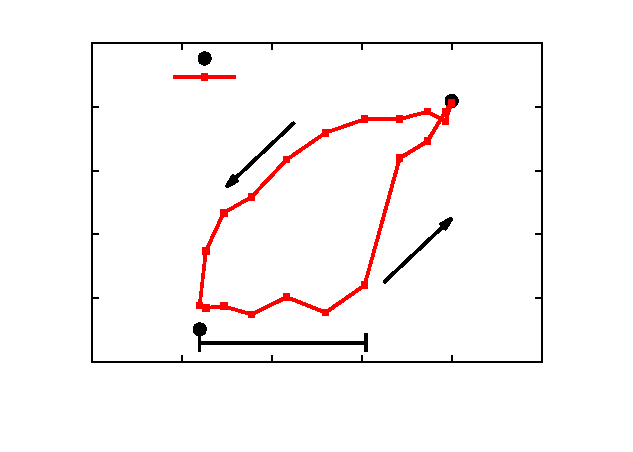
\includegraphics{sd_hys_100Hz}}%
    \gplfronttext
  \end{picture}%
\endgroup
}
  \normalsize
  \caption{Normalized displacement velocities at various inlet velocities for two steady cases and the 100 Hz oscillating unsteady cases.}
  \label{fig:sd_hys}
\end{figure}

From the steady case analysis in Sec.~\ref{sec:dynamics-V}, the dominant chemical pathways are found to be different at the leading point of the tribrachial flame and autoignition front.  Specifically, the hydrogen peroxide branching reaction (H$_2$O$_2$ + M $\Longleftrightarrow$ OH + OH + M) is the dominant chain branching reaction at the leading point of the autoignition front, while the H radical branching reaction (H + O$_2$ $\Longleftrightarrow$ O + OH) is the most important chain branching reaction at the tribrachial flame leading point.  Due to the longer residence time, hydrogen peroxide accumulation is much higher upstream of the autoignition front compared to the tribrachial flame front.

\begin{figure}[t]
  \centering
  \scriptsize
  \resizebox{0.49\textwidth}{!}{% GNUPLOT: LaTeX picture with Postscript
\begingroup
  \makeatletter
  \providecommand\color[2][]{%
    \GenericError{(gnuplot) \space\space\space\@spaces}{%
      Package color not loaded in conjunction with
      terminal option `colourtext'%
    }{See the gnuplot documentation for explanation.%
    }{Either use 'blacktext' in gnuplot or load the package
      color.sty in LaTeX.}%
    \renewcommand\color[2][]{}%
  }%
  \providecommand\includegraphics[2][]{%
    \GenericError{(gnuplot) \space\space\space\@spaces}{%
      Package graphicx or graphics not loaded%
    }{See the gnuplot documentation for explanation.%
    }{The gnuplot epslatex terminal needs graphicx.sty or graphics.sty.}%
    \renewcommand\includegraphics[2][]{}%
  }%
  \providecommand\rotatebox[2]{#2}%
  \@ifundefined{ifGPcolor}{%
    \newif\ifGPcolor
    \GPcolortrue
  }{}%
  \@ifundefined{ifGPblacktext}{%
    \newif\ifGPblacktext
    \GPblacktexttrue
  }{}%
  % define a \g@addto@macro without @ in the name:
  \let\gplgaddtomacro\g@addto@macro
  % define empty templates for all commands taking text:
  \gdef\gplbacktext{}%
  \gdef\gplfronttext{}%
  \makeatother
  \ifGPblacktext
    % no textcolor at all
    \def\colorrgb#1{}%
    \def\colorgray#1{}%
  \else
    % gray or color?
    \ifGPcolor
      \def\colorrgb#1{\color[rgb]{#1}}%
      \def\colorgray#1{\color[gray]{#1}}%
      \expandafter\def\csname LTw\endcsname{\color{white}}%
      \expandafter\def\csname LTb\endcsname{\color{black}}%
      \expandafter\def\csname LTa\endcsname{\color{black}}%
      \expandafter\def\csname LT0\endcsname{\color[rgb]{1,0,0}}%
      \expandafter\def\csname LT1\endcsname{\color[rgb]{0,1,0}}%
      \expandafter\def\csname LT2\endcsname{\color[rgb]{0,0,1}}%
      \expandafter\def\csname LT3\endcsname{\color[rgb]{1,0,1}}%
      \expandafter\def\csname LT4\endcsname{\color[rgb]{0,1,1}}%
      \expandafter\def\csname LT5\endcsname{\color[rgb]{1,1,0}}%
      \expandafter\def\csname LT6\endcsname{\color[rgb]{0,0,0}}%
      \expandafter\def\csname LT7\endcsname{\color[rgb]{1,0.3,0}}%
      \expandafter\def\csname LT8\endcsname{\color[rgb]{0.5,0.5,0.5}}%
    \else
      % gray
      \def\colorrgb#1{\color{black}}%
      \def\colorgray#1{\color[gray]{#1}}%
      \expandafter\def\csname LTw\endcsname{\color{white}}%
      \expandafter\def\csname LTb\endcsname{\color{black}}%
      \expandafter\def\csname LTa\endcsname{\color{black}}%
      \expandafter\def\csname LT0\endcsname{\color{black}}%
      \expandafter\def\csname LT1\endcsname{\color{black}}%
      \expandafter\def\csname LT2\endcsname{\color{black}}%
      \expandafter\def\csname LT3\endcsname{\color{black}}%
      \expandafter\def\csname LT4\endcsname{\color{black}}%
      \expandafter\def\csname LT5\endcsname{\color{black}}%
      \expandafter\def\csname LT6\endcsname{\color{black}}%
      \expandafter\def\csname LT7\endcsname{\color{black}}%
      \expandafter\def\csname LT8\endcsname{\color{black}}%
    \fi
  \fi
  \setlength{\unitlength}{0.0500bp}%
  \begin{picture}(4320.00,3024.00)%
    \gplgaddtomacro\gplbacktext{%
      \csname LTb\endcsname%
      \put(948,704){\makebox(0,0)[r]{\strut{}0.0e+00}}%
      \put(948,1115){\makebox(0,0)[r]{\strut{}6.0e-03}}%
      \put(948,1526){\makebox(0,0)[r]{\strut{}1.2e-02}}%
      \put(948,1937){\makebox(0,0)[r]{\strut{}1.8e-02}}%
      \put(948,2348){\makebox(0,0)[r]{\strut{}2.4e-02}}%
      \put(948,2759){\makebox(0,0)[r]{\strut{}3.0e-02}}%
      \put(1080,484){\makebox(0,0){\strut{} 0}}%
      \put(1649,484){\makebox(0,0){\strut{} 2}}%
      \put(2217,484){\makebox(0,0){\strut{} 4}}%
      \put(2786,484){\makebox(0,0){\strut{} 6}}%
      \put(3354,484){\makebox(0,0){\strut{} 8}}%
      \put(3923,484){\makebox(0,0){\strut{} 10}}%
      \put(-218,1731){\rotatebox{-270}{\makebox(0,0){\strut{}\vspace{-28pt}$Y_{\rm H_2O_2}$}}}%
      \put(2501,154){\makebox(0,0){\strut{}$x/D$}}%
      \put(1506,2896){\makebox(0,0)[l]{\strut{}$Z = 0.14$ Decreasing-velocity Cycle}}%
    }%
    \gplgaddtomacro\gplfronttext{%
      \csname LTb\endcsname%
      \put(2763,1899){\makebox(0,0)[r]{\strut{}0.5 cycle}}%
      \csname LTb\endcsname%
      \put(2763,2075){\makebox(0,0)[r]{\strut{}0.45 cycle}}%
      \csname LTb\endcsname%
      \put(2763,2251){\makebox(0,0)[r]{\strut{}0.25 cycle}}%
      \csname LTb\endcsname%
      \put(2763,2427){\makebox(0,0)[r]{\strut{}Steady 8.0 m/s}}%
      \csname LTb\endcsname%
      \put(2763,2603){\makebox(0,0)[r]{\strut{}Steady 2.4 m/s}}%
    }%
    \gplbacktext
    \put(0,0){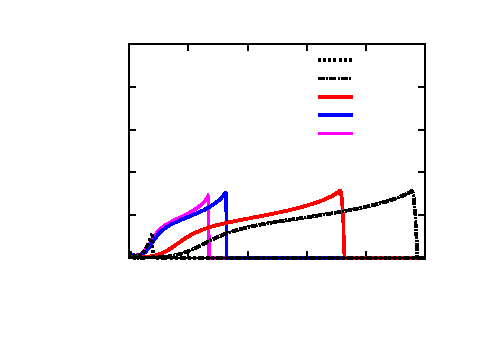
\includegraphics{H2O2_up_Z14}}%
    \gplfronttext
  \end{picture}%
\endgroup
}
  \resizebox{0.49\textwidth}{!}{% GNUPLOT: LaTeX picture with Postscript
\begingroup
  \makeatletter
  \providecommand\color[2][]{%
    \GenericError{(gnuplot) \space\space\space\@spaces}{%
      Package color not loaded in conjunction with
      terminal option `colourtext'%
    }{See the gnuplot documentation for explanation.%
    }{Either use 'blacktext' in gnuplot or load the package
      color.sty in LaTeX.}%
    \renewcommand\color[2][]{}%
  }%
  \providecommand\includegraphics[2][]{%
    \GenericError{(gnuplot) \space\space\space\@spaces}{%
      Package graphicx or graphics not loaded%
    }{See the gnuplot documentation for explanation.%
    }{The gnuplot epslatex terminal needs graphicx.sty or graphics.sty.}%
    \renewcommand\includegraphics[2][]{}%
  }%
  \providecommand\rotatebox[2]{#2}%
  \@ifundefined{ifGPcolor}{%
    \newif\ifGPcolor
    \GPcolortrue
  }{}%
  \@ifundefined{ifGPblacktext}{%
    \newif\ifGPblacktext
    \GPblacktexttrue
  }{}%
  % define a \g@addto@macro without @ in the name:
  \let\gplgaddtomacro\g@addto@macro
  % define empty templates for all commands taking text:
  \gdef\gplbacktext{}%
  \gdef\gplfronttext{}%
  \makeatother
  \ifGPblacktext
    % no textcolor at all
    \def\colorrgb#1{}%
    \def\colorgray#1{}%
  \else
    % gray or color?
    \ifGPcolor
      \def\colorrgb#1{\color[rgb]{#1}}%
      \def\colorgray#1{\color[gray]{#1}}%
      \expandafter\def\csname LTw\endcsname{\color{white}}%
      \expandafter\def\csname LTb\endcsname{\color{black}}%
      \expandafter\def\csname LTa\endcsname{\color{black}}%
      \expandafter\def\csname LT0\endcsname{\color[rgb]{1,0,0}}%
      \expandafter\def\csname LT1\endcsname{\color[rgb]{0,1,0}}%
      \expandafter\def\csname LT2\endcsname{\color[rgb]{0,0,1}}%
      \expandafter\def\csname LT3\endcsname{\color[rgb]{1,0,1}}%
      \expandafter\def\csname LT4\endcsname{\color[rgb]{0,1,1}}%
      \expandafter\def\csname LT5\endcsname{\color[rgb]{1,1,0}}%
      \expandafter\def\csname LT6\endcsname{\color[rgb]{0,0,0}}%
      \expandafter\def\csname LT7\endcsname{\color[rgb]{1,0.3,0}}%
      \expandafter\def\csname LT8\endcsname{\color[rgb]{0.5,0.5,0.5}}%
    \else
      % gray
      \def\colorrgb#1{\color{black}}%
      \def\colorgray#1{\color[gray]{#1}}%
      \expandafter\def\csname LTw\endcsname{\color{white}}%
      \expandafter\def\csname LTb\endcsname{\color{black}}%
      \expandafter\def\csname LTa\endcsname{\color{black}}%
      \expandafter\def\csname LT0\endcsname{\color{black}}%
      \expandafter\def\csname LT1\endcsname{\color{black}}%
      \expandafter\def\csname LT2\endcsname{\color{black}}%
      \expandafter\def\csname LT3\endcsname{\color{black}}%
      \expandafter\def\csname LT4\endcsname{\color{black}}%
      \expandafter\def\csname LT5\endcsname{\color{black}}%
      \expandafter\def\csname LT6\endcsname{\color{black}}%
      \expandafter\def\csname LT7\endcsname{\color{black}}%
      \expandafter\def\csname LT8\endcsname{\color{black}}%
    \fi
  \fi
  \setlength{\unitlength}{0.0500bp}%
  \begin{picture}(4320.00,3024.00)%
    \gplgaddtomacro\gplbacktext{%
      \csname LTb\endcsname%
      \put(948,704){\makebox(0,0)[r]{\strut{}0.0e+00}}%
      \put(948,1115){\makebox(0,0)[r]{\strut{}6.0e-03}}%
      \put(948,1526){\makebox(0,0)[r]{\strut{}1.2e-02}}%
      \put(948,1937){\makebox(0,0)[r]{\strut{}1.8e-02}}%
      \put(948,2348){\makebox(0,0)[r]{\strut{}2.4e-02}}%
      \put(948,2759){\makebox(0,0)[r]{\strut{}3.0e-02}}%
      \put(1080,484){\makebox(0,0){\strut{} 0}}%
      \put(1649,484){\makebox(0,0){\strut{} 2}}%
      \put(2217,484){\makebox(0,0){\strut{} 4}}%
      \put(2786,484){\makebox(0,0){\strut{} 6}}%
      \put(3354,484){\makebox(0,0){\strut{} 8}}%
      \put(3923,484){\makebox(0,0){\strut{} 10}}%
      \put(-218,1731){\rotatebox{-270}{\makebox(0,0){\strut{}\vspace{-28pt}$Y_{\rm H_2O_2}$}}}%
      \put(2501,154){\makebox(0,0){\strut{}$x/D$}}%
      \put(1506,2896){\makebox(0,0)[l]{\strut{}$Z = 0.14$ Increasing-velocity Cycle}}%
    }%
    \gplgaddtomacro\gplfronttext{%
      \csname LTb\endcsname%
      \put(2479,1547){\makebox(0,0)[r]{\strut{}0.85 cycle}}%
      \csname LTb\endcsname%
      \put(2479,1723){\makebox(0,0)[r]{\strut{}0.75 cycle}}%
      \csname LTb\endcsname%
      \put(2479,1899){\makebox(0,0)[r]{\strut{}0.65 cycle}}%
      \csname LTb\endcsname%
      \put(2479,2075){\makebox(0,0)[r]{\strut{}0.55 cycle}}%
      \csname LTb\endcsname%
      \put(2479,2251){\makebox(0,0)[r]{\strut{}0.5 cycle}}%
      \csname LTb\endcsname%
      \put(2479,2427){\makebox(0,0)[r]{\strut{}Steady 8.0 m/s}}%
      \csname LTb\endcsname%
      \put(2479,2603){\makebox(0,0)[r]{\strut{}Steady 2.4 m/s}}%
    }%
    \gplbacktext
    \put(0,0){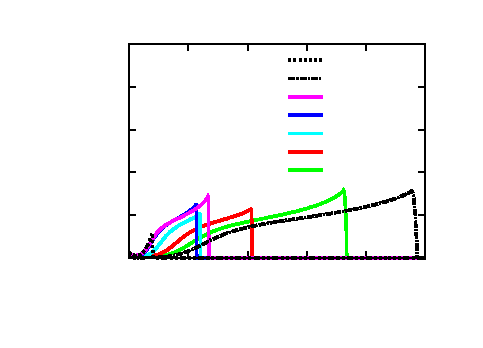
\includegraphics{ch-dynamics/H2O2_down_Z14}}%
    \gplfronttext
  \end{picture}%
\endgroup
}
  \resizebox{0.49\textwidth}{!}{% GNUPLOT: LaTeX picture with Postscript
\begingroup
  \makeatletter
  \providecommand\color[2][]{%
    \GenericError{(gnuplot) \space\space\space\@spaces}{%
      Package color not loaded in conjunction with
      terminal option `colourtext'%
    }{See the gnuplot documentation for explanation.%
    }{Either use 'blacktext' in gnuplot or load the package
      color.sty in LaTeX.}%
    \renewcommand\color[2][]{}%
  }%
  \providecommand\includegraphics[2][]{%
    \GenericError{(gnuplot) \space\space\space\@spaces}{%
      Package graphicx or graphics not loaded%
    }{See the gnuplot documentation for explanation.%
    }{The gnuplot epslatex terminal needs graphicx.sty or graphics.sty.}%
    \renewcommand\includegraphics[2][]{}%
  }%
  \providecommand\rotatebox[2]{#2}%
  \@ifundefined{ifGPcolor}{%
    \newif\ifGPcolor
    \GPcolortrue
  }{}%
  \@ifundefined{ifGPblacktext}{%
    \newif\ifGPblacktext
    \GPblacktexttrue
  }{}%
  % define a \g@addto@macro without @ in the name:
  \let\gplgaddtomacro\g@addto@macro
  % define empty templates for all commands taking text:
  \gdef\gplbacktext{}%
  \gdef\gplfronttext{}%
  \makeatother
  \ifGPblacktext
    % no textcolor at all
    \def\colorrgb#1{}%
    \def\colorgray#1{}%
  \else
    % gray or color?
    \ifGPcolor
      \def\colorrgb#1{\color[rgb]{#1}}%
      \def\colorgray#1{\color[gray]{#1}}%
      \expandafter\def\csname LTw\endcsname{\color{white}}%
      \expandafter\def\csname LTb\endcsname{\color{black}}%
      \expandafter\def\csname LTa\endcsname{\color{black}}%
      \expandafter\def\csname LT0\endcsname{\color[rgb]{1,0,0}}%
      \expandafter\def\csname LT1\endcsname{\color[rgb]{0,1,0}}%
      \expandafter\def\csname LT2\endcsname{\color[rgb]{0,0,1}}%
      \expandafter\def\csname LT3\endcsname{\color[rgb]{1,0,1}}%
      \expandafter\def\csname LT4\endcsname{\color[rgb]{0,1,1}}%
      \expandafter\def\csname LT5\endcsname{\color[rgb]{1,1,0}}%
      \expandafter\def\csname LT6\endcsname{\color[rgb]{0,0,0}}%
      \expandafter\def\csname LT7\endcsname{\color[rgb]{1,0.3,0}}%
      \expandafter\def\csname LT8\endcsname{\color[rgb]{0.5,0.5,0.5}}%
    \else
      % gray
      \def\colorrgb#1{\color{black}}%
      \def\colorgray#1{\color[gray]{#1}}%
      \expandafter\def\csname LTw\endcsname{\color{white}}%
      \expandafter\def\csname LTb\endcsname{\color{black}}%
      \expandafter\def\csname LTa\endcsname{\color{black}}%
      \expandafter\def\csname LT0\endcsname{\color{black}}%
      \expandafter\def\csname LT1\endcsname{\color{black}}%
      \expandafter\def\csname LT2\endcsname{\color{black}}%
      \expandafter\def\csname LT3\endcsname{\color{black}}%
      \expandafter\def\csname LT4\endcsname{\color{black}}%
      \expandafter\def\csname LT5\endcsname{\color{black}}%
      \expandafter\def\csname LT6\endcsname{\color{black}}%
      \expandafter\def\csname LT7\endcsname{\color{black}}%
      \expandafter\def\csname LT8\endcsname{\color{black}}%
    \fi
  \fi
  \setlength{\unitlength}{0.0500bp}%
  \begin{picture}(4320.00,3024.00)%
    \gplgaddtomacro\gplbacktext{%
      \csname LTb\endcsname%
      \put(948,704){\makebox(0,0)[r]{\strut{}0.0e+00}}%
      \put(948,1115){\makebox(0,0)[r]{\strut{}6.0e-03}}%
      \put(948,1526){\makebox(0,0)[r]{\strut{}1.2e-02}}%
      \put(948,1937){\makebox(0,0)[r]{\strut{}1.8e-02}}%
      \put(948,2348){\makebox(0,0)[r]{\strut{}2.4e-02}}%
      \put(948,2759){\makebox(0,0)[r]{\strut{}3.0e-02}}%
      \put(1080,484){\makebox(0,0){\strut{} 0}}%
      \put(1649,484){\makebox(0,0){\strut{} 2}}%
      \put(2217,484){\makebox(0,0){\strut{} 4}}%
      \put(2786,484){\makebox(0,0){\strut{} 6}}%
      \put(3354,484){\makebox(0,0){\strut{} 8}}%
      \put(3923,484){\makebox(0,0){\strut{} 10}}%
      \put(-218,1731){\rotatebox{-270}{\makebox(0,0){\strut{}\vspace{-28pt}$Y_{\rm H_2O_2}$}}}%
      \put(2501,154){\makebox(0,0){\strut{}$x/D$}}%
      \put(1506,2896){\makebox(0,0)[l]{\strut{}$Z = 0.24$ Decreasing-velocity Cycle}}%
    }%
    \gplgaddtomacro\gplfronttext{%
      \csname LTb\endcsname%
      \put(2763,1899){\makebox(0,0)[r]{\strut{}0.5 cycle}}%
      \csname LTb\endcsname%
      \put(2763,2075){\makebox(0,0)[r]{\strut{}0.45 cycle}}%
      \csname LTb\endcsname%
      \put(2763,2251){\makebox(0,0)[r]{\strut{}0.25 cycle}}%
      \csname LTb\endcsname%
      \put(2763,2427){\makebox(0,0)[r]{\strut{}Steady 8.0 m/s}}%
      \csname LTb\endcsname%
      \put(2763,2603){\makebox(0,0)[r]{\strut{}Steady 2.4 m/s}}%
    }%
    \gplbacktext
    \put(0,0){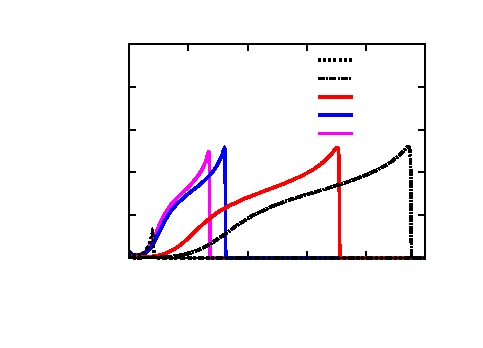
\includegraphics{ch-dynamics/H2O2_up_Z24}}%
    \gplfronttext
  \end{picture}%
\endgroup
}
  \resizebox{0.49\textwidth}{!}{% GNUPLOT: LaTeX picture with Postscript
\begingroup
  \makeatletter
  \providecommand\color[2][]{%
    \GenericError{(gnuplot) \space\space\space\@spaces}{%
      Package color not loaded in conjunction with
      terminal option `colourtext'%
    }{See the gnuplot documentation for explanation.%
    }{Either use 'blacktext' in gnuplot or load the package
      color.sty in LaTeX.}%
    \renewcommand\color[2][]{}%
  }%
  \providecommand\includegraphics[2][]{%
    \GenericError{(gnuplot) \space\space\space\@spaces}{%
      Package graphicx or graphics not loaded%
    }{See the gnuplot documentation for explanation.%
    }{The gnuplot epslatex terminal needs graphicx.sty or graphics.sty.}%
    \renewcommand\includegraphics[2][]{}%
  }%
  \providecommand\rotatebox[2]{#2}%
  \@ifundefined{ifGPcolor}{%
    \newif\ifGPcolor
    \GPcolortrue
  }{}%
  \@ifundefined{ifGPblacktext}{%
    \newif\ifGPblacktext
    \GPblacktexttrue
  }{}%
  % define a \g@addto@macro without @ in the name:
  \let\gplgaddtomacro\g@addto@macro
  % define empty templates for all commands taking text:
  \gdef\gplbacktext{}%
  \gdef\gplfronttext{}%
  \makeatother
  \ifGPblacktext
    % no textcolor at all
    \def\colorrgb#1{}%
    \def\colorgray#1{}%
  \else
    % gray or color?
    \ifGPcolor
      \def\colorrgb#1{\color[rgb]{#1}}%
      \def\colorgray#1{\color[gray]{#1}}%
      \expandafter\def\csname LTw\endcsname{\color{white}}%
      \expandafter\def\csname LTb\endcsname{\color{black}}%
      \expandafter\def\csname LTa\endcsname{\color{black}}%
      \expandafter\def\csname LT0\endcsname{\color[rgb]{1,0,0}}%
      \expandafter\def\csname LT1\endcsname{\color[rgb]{0,1,0}}%
      \expandafter\def\csname LT2\endcsname{\color[rgb]{0,0,1}}%
      \expandafter\def\csname LT3\endcsname{\color[rgb]{1,0,1}}%
      \expandafter\def\csname LT4\endcsname{\color[rgb]{0,1,1}}%
      \expandafter\def\csname LT5\endcsname{\color[rgb]{1,1,0}}%
      \expandafter\def\csname LT6\endcsname{\color[rgb]{0,0,0}}%
      \expandafter\def\csname LT7\endcsname{\color[rgb]{1,0.3,0}}%
      \expandafter\def\csname LT8\endcsname{\color[rgb]{0.5,0.5,0.5}}%
    \else
      % gray
      \def\colorrgb#1{\color{black}}%
      \def\colorgray#1{\color[gray]{#1}}%
      \expandafter\def\csname LTw\endcsname{\color{white}}%
      \expandafter\def\csname LTb\endcsname{\color{black}}%
      \expandafter\def\csname LTa\endcsname{\color{black}}%
      \expandafter\def\csname LT0\endcsname{\color{black}}%
      \expandafter\def\csname LT1\endcsname{\color{black}}%
      \expandafter\def\csname LT2\endcsname{\color{black}}%
      \expandafter\def\csname LT3\endcsname{\color{black}}%
      \expandafter\def\csname LT4\endcsname{\color{black}}%
      \expandafter\def\csname LT5\endcsname{\color{black}}%
      \expandafter\def\csname LT6\endcsname{\color{black}}%
      \expandafter\def\csname LT7\endcsname{\color{black}}%
      \expandafter\def\csname LT8\endcsname{\color{black}}%
    \fi
  \fi
  \setlength{\unitlength}{0.0500bp}%
  \begin{picture}(4320.00,3024.00)%
    \gplgaddtomacro\gplbacktext{%
      \csname LTb\endcsname%
      \put(948,704){\makebox(0,0)[r]{\strut{}0.0e+00}}%
      \put(948,1115){\makebox(0,0)[r]{\strut{}6.0e-03}}%
      \put(948,1526){\makebox(0,0)[r]{\strut{}1.2e-02}}%
      \put(948,1937){\makebox(0,0)[r]{\strut{}1.8e-02}}%
      \put(948,2348){\makebox(0,0)[r]{\strut{}2.4e-02}}%
      \put(948,2759){\makebox(0,0)[r]{\strut{}3.0e-02}}%
      \put(1080,484){\makebox(0,0){\strut{} 0}}%
      \put(1649,484){\makebox(0,0){\strut{} 2}}%
      \put(2217,484){\makebox(0,0){\strut{} 4}}%
      \put(2786,484){\makebox(0,0){\strut{} 6}}%
      \put(3354,484){\makebox(0,0){\strut{} 8}}%
      \put(3923,484){\makebox(0,0){\strut{} 10}}%
      \put(-218,1731){\rotatebox{-270}{\makebox(0,0){\strut{}\vspace{-28pt}$Y_{\rm H_2O_2}$}}}%
      \put(2501,154){\makebox(0,0){\strut{}$x/D$}}%
      \put(1506,2896){\makebox(0,0)[l]{\strut{}$Z = 0.24$ Increasing-velocity Cycle}}%
    }%
    \gplgaddtomacro\gplfronttext{%
      \csname LTb\endcsname%
      \put(2479,1547){\makebox(0,0)[r]{\strut{}0.85 cycle}}%
      \csname LTb\endcsname%
      \put(2479,1723){\makebox(0,0)[r]{\strut{}0.75 cycle}}%
      \csname LTb\endcsname%
      \put(2479,1899){\makebox(0,0)[r]{\strut{}0.65 cycle}}%
      \csname LTb\endcsname%
      \put(2479,2075){\makebox(0,0)[r]{\strut{}0.55 cycle}}%
      \csname LTb\endcsname%
      \put(2479,2251){\makebox(0,0)[r]{\strut{}0.5 cycle}}%
      \csname LTb\endcsname%
      \put(2479,2427){\makebox(0,0)[r]{\strut{}Steady 8.0 m/s}}%
      \csname LTb\endcsname%
      \put(2479,2603){\makebox(0,0)[r]{\strut{}Steady 2.4 m/s}}%
    }%
    \gplbacktext
    \put(0,0){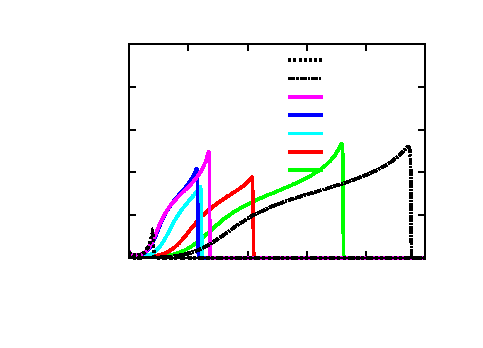
\includegraphics{H2O2_down_Z24}}%
    \gplfronttext
  \end{picture}%
\endgroup
}
  \normalsize
  \caption{Comparison of hydrogen peroxide mass fraction profiles along the $Z = 0.14$ and $Z = 0.24$ iso-contours at steady state and at $100$ Hz during the decreasing-velocity cycle (left) and increasing-velocity cycle (right).}
  \label{fig:H2O2_updown}
\end{figure}

As hydrogen peroxide plays different roles in the tribrachial flame and autoignition front, its spatial profiles along the $Z = 0.14$ and $Z = 0.24$ iso-contours are compared in Fig.~\ref{fig:H2O2_updown}, with the left and right subfigures corresponding to the decreasing-velocity and increasing-velocity half cycles, respectively.  Qualitatively, the evolution of the hydrogen peroxide profiles shows similar trends along both mixture fraction iso-contours.  The left figures show that hydrogen peroxide accumulates until either autoignition occurs or it is consumed at the flame front, resulting in a sharp drop in its mass fraction.  However, depending on the mixture fraction, the peak value of the hydrogen peroxide mass fraction differs by three to five times between a steady autoignition front (the steady 8.0 m/s case) and a tribrachial flame (the steady 2.4 m/s case), which implies its different significance in these two combustion modes and sets the benchmark for the unsteady evolution.  As the inlet velocity decreases from $8.0$ m/s, the peak $Y_{\rm H{_2}O{_2}}$ almost remains constant, indicating that the chemical structure is very close to the steady autoignition case.  As a consequence, the dominant chemical pathway remains H$_2$O$_2$ + M $\Longleftrightarrow$ OH + OH + M, and autoignition is the dominant combustion process, resulting in larger $S_d/S_L$.  However, as the flow velocity decreases, a larger gradient is achieved, resulting in steeper profiles and smaller $S_d/S_L$, according to Eq.~(\ref{eq:sd}).  The large gradient results in enhanced back diffusion from the reacting front to the unburnt upstream mixture and ultimately drives the transition into a tribrachial flame.

Even when the inlet velocity reaches the minimum $2.4$ m/s, which is the same as the steady case, the reacting front continues to move upstream.  Inlet velocity changes slowest around the half cycle, allowing the chemical structure to respond to the hydrodynamic changes.  As shown on the right of Fig.~\ref{fig:H2O2_updown}, the peak $Y_{\rm H{_2}O{_2}}$ decreases from $0.5$ to $0.65$ of the cycle.  At this stage, autoignition is not fully activated, since the peak $Y_{\rm H{_2}O{_2}}$ is lower than the steady autoignition case.  However, the peak $Y_{\rm H{_2}O{_2}}$ is still larger than the steady tribrachial flame.  Therefore, the $S_d/S_L$ of the tribrachial structure is close to but slightly larger than a steady flame, for it is propagating into a partially reacted mixture.  

As the inlet velocity further increases from $0.65$ to $0.75$ of the cycle, the propagation speed of the tribrachial flame cannot keep up with the flow incoming velocity, and the flame structure is therefore convected downstream.  During this flame blow-off process, $S_d/S_L$ remains essentially constant, which is demonstrated as the flattened bottom in Fig.~\ref{fig:sd_hys}.  Meanwhile, the unburnt mixture upstream of the flame accumulates radicals and heat as it moves downstream and eventually triggers autoignition, indicated by a sudden jump of $S_d/S_L$.  The time difference between the half cycle (where the inlet velocity is 2.4 m/s) and the last sample point before the sudden jump of $S_d/S_L$ is defined as the induction period, as indicated in Fig.~\ref{fig:sd_hys}.

\subsection{Effects of Oscillation Frequency} \label{sec:frq}

To better understand the coupling between hydrodynamics and chemistry and the hysteretic behavior in Fig.~\ref{fig:sd_hys}, the effects of oscillation frequency are analyzed.  Compared to the $100$ Hz case, the other two cases of lower oscillation frequency are similar qualitatively but with some quantitative differences.  Figure~\ref{fig:xd_evo} shows the evolution of the normalized leading point location ($x_d/D$) for the three oscillating cases, compared with the steady benchmark cases.  The peak-to-peak variation represents the oscillation amplitude during a cycle.  Two distinct trends are evident.  First, as the oscillation frequency increases, the oscillation amplitude decreases.  Extrapolating, if the oscillation frequency were much faster than any chemical or transport times scale, the oscillation amplitude would be zero, since the thermal structure could not respond to the velocity changes.

Second and more interestingly, for all three frequencies, the most downstream points during the oscillation are almost identical to the steady case at 8.0 m/s.  However, as the frequency increases, the most upstream point during the oscillation deviates more from the steady case at 2.4 m/s.  The different effects of oscillation frequency on the most downstream and upstream points are attributed to the difference in the combustion mode at these two locations.  As demonstrated in Fig.~\ref{fig:sd_hys}, the 100 Hz oscillating case has already established quasi-steady state when the boundary velocity is at 8.0 m/s when the combustion mode is kinetically controlled by autoignition.  In a Lagrangian sense, the location of an autoignition front is directly related to the ignition delay time, determined by chemical kinetics.  Therefore, the location of the autoignition front at this quasi-steady state is almost the same as the steady case with the same boundary velocity, which can be crudely estimated as the product of the ignition delay time and the boundary velocity.  For even lower frequency cases, such a quasi-steady state is even easier to achieve.  Consequently, for all three oscillation frequencies, the most downstream points remain very close to the steady autoignition governed case with the boundary velocity of 8.0 m/s.  Conversely, the stabilization mechanism for the steady case at 2.4 m/s is kinematically controlled by the balance between the tribrachial flame propagation speed and the incoming flow speed.  For the 100 Hz case, however, such kinematic balance never achieves quasi-steady state, as discussed in the previous section.  The location of the tribrachial flame is then determined kinematically both by the velocity difference between the unsteady tribrachial flame propagation speed and the flow speed and the time allowed for such displacement to occur.  At lower oscillation frequencies, longer time is allowed for the tribrachial flame to propagate upstream into the partially reacted mixture, while the displacement velocity decreases gradually due to reduced reactivity upstream.  The most upstream point location will then asymptotically approaches the steady state case when the oscillation frequency is sufficiently low.  This explains why the minimum $x_d/D$ approaches the steady state case at 2.4 m/s more closely at lower oscillation frequency in Fig.~\ref{fig:xd_evo}.

\begin{figure}[t]
  \centering
  \scriptsize
  \resizebox{1.0\textwidth}{!}{% GNUPLOT: LaTeX picture with Postscript
\begingroup
  \makeatletter
  \providecommand\color[2][]{%
    \GenericError{(gnuplot) \space\space\space\@spaces}{%
      Package color not loaded in conjunction with
      terminal option `colourtext'%
    }{See the gnuplot documentation for explanation.%
    }{Either use 'blacktext' in gnuplot or load the package
      color.sty in LaTeX.}%
    \renewcommand\color[2][]{}%
  }%
  \providecommand\includegraphics[2][]{%
    \GenericError{(gnuplot) \space\space\space\@spaces}{%
      Package graphicx or graphics not loaded%
    }{See the gnuplot documentation for explanation.%
    }{The gnuplot epslatex terminal needs graphicx.sty or graphics.sty.}%
    \renewcommand\includegraphics[2][]{}%
  }%
  \providecommand\rotatebox[2]{#2}%
  \@ifundefined{ifGPcolor}{%
    \newif\ifGPcolor
    \GPcolortrue
  }{}%
  \@ifundefined{ifGPblacktext}{%
    \newif\ifGPblacktext
    \GPblacktexttrue
  }{}%
  % define a \g@addto@macro without @ in the name:
  \let\gplgaddtomacro\g@addto@macro
  % define empty templates for all commands taking text:
  \gdef\gplbacktext{}%
  \gdef\gplfronttext{}%
  \makeatother
  \ifGPblacktext
    % no textcolor at all
    \def\colorrgb#1{}%
    \def\colorgray#1{}%
  \else
    % gray or color?
    \ifGPcolor
      \def\colorrgb#1{\color[rgb]{#1}}%
      \def\colorgray#1{\color[gray]{#1}}%
      \expandafter\def\csname LTw\endcsname{\color{white}}%
      \expandafter\def\csname LTb\endcsname{\color{black}}%
      \expandafter\def\csname LTa\endcsname{\color{black}}%
      \expandafter\def\csname LT0\endcsname{\color[rgb]{1,0,0}}%
      \expandafter\def\csname LT1\endcsname{\color[rgb]{0,1,0}}%
      \expandafter\def\csname LT2\endcsname{\color[rgb]{0,0,1}}%
      \expandafter\def\csname LT3\endcsname{\color[rgb]{1,0,1}}%
      \expandafter\def\csname LT4\endcsname{\color[rgb]{0,1,1}}%
      \expandafter\def\csname LT5\endcsname{\color[rgb]{1,1,0}}%
      \expandafter\def\csname LT6\endcsname{\color[rgb]{0,0,0}}%
      \expandafter\def\csname LT7\endcsname{\color[rgb]{1,0.3,0}}%
      \expandafter\def\csname LT8\endcsname{\color[rgb]{0.5,0.5,0.5}}%
    \else
      % gray
      \def\colorrgb#1{\color{black}}%
      \def\colorgray#1{\color[gray]{#1}}%
      \expandafter\def\csname LTw\endcsname{\color{white}}%
      \expandafter\def\csname LTb\endcsname{\color{black}}%
      \expandafter\def\csname LTa\endcsname{\color{black}}%
      \expandafter\def\csname LT0\endcsname{\color{black}}%
      \expandafter\def\csname LT1\endcsname{\color{black}}%
      \expandafter\def\csname LT2\endcsname{\color{black}}%
      \expandafter\def\csname LT3\endcsname{\color{black}}%
      \expandafter\def\csname LT4\endcsname{\color{black}}%
      \expandafter\def\csname LT5\endcsname{\color{black}}%
      \expandafter\def\csname LT6\endcsname{\color{black}}%
      \expandafter\def\csname LT7\endcsname{\color{black}}%
      \expandafter\def\csname LT8\endcsname{\color{black}}%
    \fi
  \fi
  \setlength{\unitlength}{0.0500bp}%
  \begin{picture}(5760.00,4032.00)%
    \gplgaddtomacro\gplbacktext{%
      \csname LTb\endcsname%
      \put(588,704){\makebox(0,0)[r]{\strut{} 0}}%
      \put(588,1317){\makebox(0,0)[r]{\strut{} 3}}%
      \put(588,1929){\makebox(0,0)[r]{\strut{} 6}}%
      \put(588,2542){\makebox(0,0)[r]{\strut{} 9}}%
      \put(588,3154){\makebox(0,0)[r]{\strut{} 12}}%
      \put(588,3767){\makebox(0,0)[r]{\strut{} 15}}%
      \put(720,484){\makebox(0,0){\strut{} 0}}%
      \put(1260,484){\makebox(0,0){\strut{} 0.25}}%
      \put(1800,484){\makebox(0,0){\strut{} 0.5}}%
      \put(2340,484){\makebox(0,0){\strut{} 0.75}}%
      \put(2880,484){\makebox(0,0){\strut{} 1}}%
      \put(3419,484){\makebox(0,0){\strut{} 1.25}}%
      \put(3959,484){\makebox(0,0){\strut{} 1.5}}%
      \put(4499,484){\makebox(0,0){\strut{} 1.75}}%
      \put(5039,484){\makebox(0,0){\strut{} 2}}%
      \put(-50,2235){\rotatebox{-270}{\makebox(0,0){\strut{}\vspace{-28pt}$x_d/D$}}}%
      \put(2879,154){\makebox(0,0){\strut{}Cycle}}%
    }%
    \gplgaddtomacro\gplfronttext{%
      \csname LTb\endcsname%
      \put(2068,3577){\makebox(0,0)[r]{\strut{}Steady 2.4 m/s}}%
      \csname LTb\endcsname%
      \put(2068,3401){\makebox(0,0)[r]{\strut{}Steady 8.0 m/s}}%
      \csname LTb\endcsname%
      \put(2068,3225){\makebox(0,0)[r]{\strut{}100 Hz}}%
      \csname LTb\endcsname%
      \put(2068,3049){\makebox(0,0)[r]{\strut{}50 Hz}}%
      \csname LTb\endcsname%
      \put(2068,2873){\makebox(0,0)[r]{\strut{}25 Hz}}%
    }%
    \gplbacktext
    \put(0,0){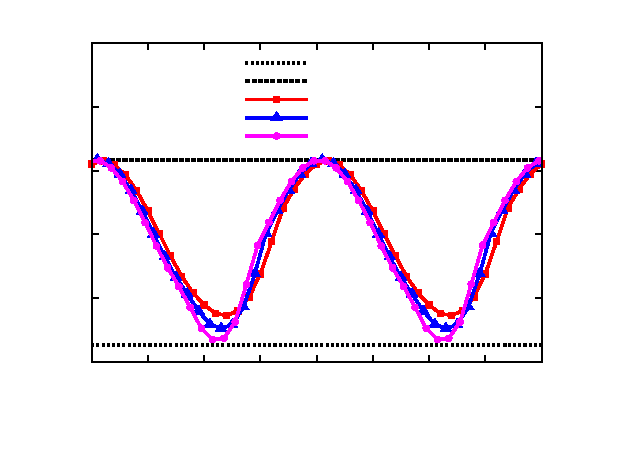
\includegraphics{xd_evo}}%
    \gplfronttext
  \end{picture}%
\endgroup
}
  \normalsize
  \caption{Normalized leading point location time history profiles at 25, 50, and 100 Hz.}
  \label{fig:xd_evo}
\end{figure}    

Besides the oscillation amplitude, the hysteretic behavior is also affected by the oscillation frequency.  As shown in Fig.~\ref{fig:sd_hys_frq}, the hysteresis of decreasing and increasing velocity is diminished as the oscillation frequency decreases, denoted by the shrinking of the enclosed area.  Hysteresis remains at slower inlet velocities since the decreasing-velocity branch is still autoignition dominated, but it takes finite induction time for the increasing-velocity unburnt mixture to achieve autoignition.  At higher inlet velocities, both branches are autoignition dominant and therefore collapse to a single path at sufficiently low frequency, approaching the quasi-steady limit.  Ideally, the quasi-steady limit could be achieved by investigating even lower frequencies, such as 0.1 Hz; however, such calculation would be extraordinarily intensive, requiring more than 20 million core-hours.  Instead, three steady state cases reported previously in Sec.~\ref{sec:dynamics-V} and a new steady case at the boundary velocity of 6.4 m/s are also included in Fig.~\ref{fig:sd_hys_frq} to illustrate the steady state limit.  The 3.2 m/s case is kinematically stabilized, similar to the 2.4 m/s case, and therefore is closer to the increasing-velocity branches of the oscillating cases but is different from the decreasing-velocity branches for the same reason at the lower velocity condition, as discussed in the previous section.  Conversely, the 6.4 m/s case is kinetically stabilized by autoignition, which can be approached by both the decreasing-velocity and increasing-velocity branches at lower oscillation frequency.

\begin{figure}[t]
  \centering
  \scriptsize
  \resizebox{1.0\textwidth}{!}{% GNUPLOT: LaTeX picture with Postscript
\begingroup
  \makeatletter
  \providecommand\color[2][]{%
    \GenericError{(gnuplot) \space\space\space\@spaces}{%
      Package color not loaded in conjunction with
      terminal option `colourtext'%
    }{See the gnuplot documentation for explanation.%
    }{Either use 'blacktext' in gnuplot or load the package
      color.sty in LaTeX.}%
    \renewcommand\color[2][]{}%
  }%
  \providecommand\includegraphics[2][]{%
    \GenericError{(gnuplot) \space\space\space\@spaces}{%
      Package graphicx or graphics not loaded%
    }{See the gnuplot documentation for explanation.%
    }{The gnuplot epslatex terminal needs graphicx.sty or graphics.sty.}%
    \renewcommand\includegraphics[2][]{}%
  }%
  \providecommand\rotatebox[2]{#2}%
  \@ifundefined{ifGPcolor}{%
    \newif\ifGPcolor
    \GPcolortrue
  }{}%
  \@ifundefined{ifGPblacktext}{%
    \newif\ifGPblacktext
    \GPblacktexttrue
  }{}%
  % define a \g@addto@macro without @ in the name:
  \let\gplgaddtomacro\g@addto@macro
  % define empty templates for all commands taking text:
  \gdef\gplbacktext{}%
  \gdef\gplfronttext{}%
  \makeatother
  \ifGPblacktext
    % no textcolor at all
    \def\colorrgb#1{}%
    \def\colorgray#1{}%
  \else
    % gray or color?
    \ifGPcolor
      \def\colorrgb#1{\color[rgb]{#1}}%
      \def\colorgray#1{\color[gray]{#1}}%
      \expandafter\def\csname LTw\endcsname{\color{white}}%
      \expandafter\def\csname LTb\endcsname{\color{black}}%
      \expandafter\def\csname LTa\endcsname{\color{black}}%
      \expandafter\def\csname LT0\endcsname{\color[rgb]{1,0,0}}%
      \expandafter\def\csname LT1\endcsname{\color[rgb]{0,1,0}}%
      \expandafter\def\csname LT2\endcsname{\color[rgb]{0,0,1}}%
      \expandafter\def\csname LT3\endcsname{\color[rgb]{1,0,1}}%
      \expandafter\def\csname LT4\endcsname{\color[rgb]{0,1,1}}%
      \expandafter\def\csname LT5\endcsname{\color[rgb]{1,1,0}}%
      \expandafter\def\csname LT6\endcsname{\color[rgb]{0,0,0}}%
      \expandafter\def\csname LT7\endcsname{\color[rgb]{1,0.3,0}}%
      \expandafter\def\csname LT8\endcsname{\color[rgb]{0.5,0.5,0.5}}%
    \else
      % gray
      \def\colorrgb#1{\color{black}}%
      \def\colorgray#1{\color[gray]{#1}}%
      \expandafter\def\csname LTw\endcsname{\color{white}}%
      \expandafter\def\csname LTb\endcsname{\color{black}}%
      \expandafter\def\csname LTa\endcsname{\color{black}}%
      \expandafter\def\csname LT0\endcsname{\color{black}}%
      \expandafter\def\csname LT1\endcsname{\color{black}}%
      \expandafter\def\csname LT2\endcsname{\color{black}}%
      \expandafter\def\csname LT3\endcsname{\color{black}}%
      \expandafter\def\csname LT4\endcsname{\color{black}}%
      \expandafter\def\csname LT5\endcsname{\color{black}}%
      \expandafter\def\csname LT6\endcsname{\color{black}}%
      \expandafter\def\csname LT7\endcsname{\color{black}}%
      \expandafter\def\csname LT8\endcsname{\color{black}}%
    \fi
  \fi
  \setlength{\unitlength}{0.0500bp}%
  \begin{picture}(5760.00,4032.00)%
    \gplgaddtomacro\gplbacktext{%
      \csname LTb\endcsname%
      \put(588,704){\makebox(0,0)[r]{\strut{} 0}}%
      \put(588,1317){\makebox(0,0)[r]{\strut{} 2}}%
      \put(588,1929){\makebox(0,0)[r]{\strut{} 4}}%
      \put(588,2542){\makebox(0,0)[r]{\strut{} 6}}%
      \put(588,3154){\makebox(0,0)[r]{\strut{} 8}}%
      \put(588,3767){\makebox(0,0)[r]{\strut{} 10}}%
      \put(720,484){\makebox(0,0){\strut{} 0}}%
      \put(1584,484){\makebox(0,0){\strut{} 2}}%
      \put(2448,484){\makebox(0,0){\strut{} 4}}%
      \put(3311,484){\makebox(0,0){\strut{} 6}}%
      \put(4175,484){\makebox(0,0){\strut{} 8}}%
      \put(5039,484){\makebox(0,0){\strut{} 10}}%
      \put(-50,2235){\rotatebox{-270}{\makebox(0,0){\strut{}\vspace{-28pt}$S_d/S_L$}}}%
      \put(2879,154){\makebox(0,0){\strut{}$U_{\rm inlet}$}}%
      \put(1066,2848){\makebox(0,0)[l]{\strut{}Decreasing-velocity}}%
      \put(3743,1470){\makebox(0,0)[l]{\strut{}Increasing-velocity}}%
    }%
    \gplgaddtomacro\gplfronttext{%
      \csname LTb\endcsname%
      \put(1377,3618){\makebox(0,0)[r]{\strut{}Steady}}%
      \csname LTb\endcsname%
      \put(1377,3442){\makebox(0,0)[r]{\strut{}100 Hz}}%
      \csname LTb\endcsname%
      \put(1377,3266){\makebox(0,0)[r]{\strut{}50 Hz}}%
      \csname LTb\endcsname%
      \put(1377,3090){\makebox(0,0)[r]{\strut{}25 Hz}}%
    }%
    \gplbacktext
    \put(0,0){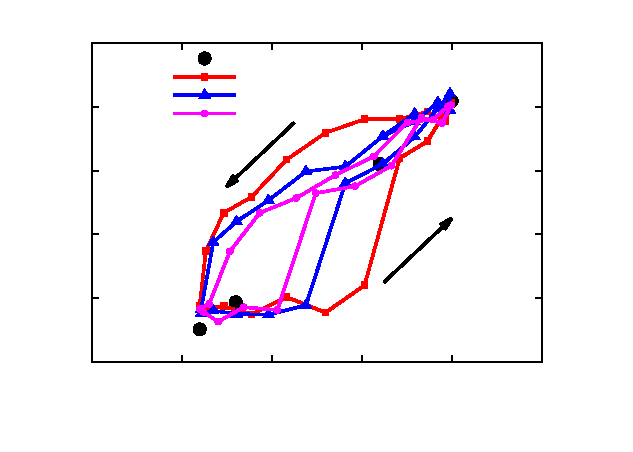
\includegraphics{sd_hys_frq}}%
    \gplfronttext
  \end{picture}%
\endgroup
}
  \normalsize
  \caption{Normalized displacement velocities at various inlet velocities for four steady cases and three oscillating unsteady cases at different frequencies.  Induction periods for the unsteady cases can also been defined similar to Fig.~\ref{fig:sd_hys} but are not shown here for clarity.}
  \label{fig:sd_hys_frq}
\end{figure}

In terms of the relative portion of the oscillation cycle, the 100 Hz case demonstrates a more pronounced hysteresis and longer induction period.  However, in term of the absolute time, shown in Table~\ref{table:ind}, the 25 Hz case takes a longer time to achieve the transition from small $S_d/S_L$ to larger values during the increasing-velocity portion of the cycle , noting that the time intervals between sampling points in Fig.~\ref{fig:sd_hys_frq} are not the same for the three frequencies, being $0.5$, $1.0$, and $2.0$ ms for 100, 50, and 25 Hz, respectively.

\begin{table*}
  \caption{Induction time at different harmonic oscillation frequencies.  The definition of the induction time is illustrated in Fig.~\ref{fig:sd_hys}}
  \label{table:ind}
  \centering
  \normalsize
  \resizebox{0.6\textwidth}{!}{
  \begin{tabular}{lc*{2}{c}}
    \hline
    Frequency [Hz]& $25$  & $50$  & $100$   \\
    \hline
    Induction Time [ms]& $6$ & $4$ & $2.5$\\
    \hline
   \end{tabular}
}
\end{table*}

This counter-intuitive finding is explained with Fig.~\ref{fig:ind_frq}.  Here, the temperature, hydrogen peroxide, and methoxymethylperoxy radical (CH$_3$OCH$_2$O$_2$) profiles are compared for the three frequency cases for both decreasing- and increasing-velocity branches at the same inlet velocity of $3.2$ m/s and benchmarked with the corresponding steady computation.  As in Secs.~\ref{sec:dynamics-T} and~\ref{sec:dynamics-V}, this steady case is autoignition dominated and stabilized at $Z = 0.24$.  

According to the temperature profiles, the steady and unsteady cases all demonstrate two heat release stages, with the first and second stage correlated well with the depletion of the CH$_3$OCH$_2$O$_2$ radical and hydrogen peroxide, respectively.  The CH$_3$OCH$_2$O$_2$ radical is often chosen to represent the NTC chemistry~\cite{krisman15}.  As demonstrated in the steady cases, NTC chemistry is important in the upstream of both tribrachial flame and autoignition front, and NTC chemistry is still important for the unsteady cases.  It is seen from Fig.~\ref{fig:ind_frq} that, irrespective of the oscillation frequency and traveling direction, at the same inlet velocity, $Y_{\rm CH_3OCH_2O_2}$ matches with its steady state profile, indicating that NTC chemistry responds to the flow oscillation relatively fast, and therefore is decoupled from flow dynamics.

Conversely, the coupling between fluid dynamics and second-stage autoignition/flame chemistry is important, for the hydrogen peroxide profiles of the unsteady cases fail to collapse onto that of the steady case.  Although three unsteady profiles on the decreasing-velocity branch show similar peak values, the lower the frequency, the closer the profile matches the steady case, which is expected from Fig.~\ref{fig:sd_hys_frq}.  However, the unsteady profiles on the increasing-velocity branch show lower peak values than the steady structure, with the $100$ Hz case profile being closer to the steady counterpart.  Noting from Fig.~\ref{fig:sd_hys_frq} that the minimum $S_d/S_L$ in all three cases are larger than the steady $2.4$ m/s case and at lower frequency the unburnt mixture has longer time to relax to steady state, the $25$ Hz case should match the $2.4$ m/s steady case closer, that is, a tribrachial flame with low H$_2$O$_2$ accumulation.  Therefore, a longer time is required to accumulate this lost H$_2$O$_2$ and activate autoignition.  Conversely, the $100$ Hz case allows less time to relax to a steady flame structure and therefore has larger $Y_{\rm H_2O_2}$ to start with during the increasing-velocity cycle, resulting in a shorter induction time for autoignition.

The different effects of oscillation frequency on the first-stage NTC chemistry and second-stage autoignition/flame chemistry can be understood by comparing the characteristic time scales of these processes.  The ignition delay time for the first-stage ignition facilitated by NTC chemistry is relatively short ($\sim$0.3 ms, according to Sec.~\ref{sec:dynamics-V}) compared to the major autoignition process induced by the hydrogen peroxide branching reaction ($\sim$1 ms, according to Sec.~\ref{sec:dynamics-V}) and the characteristic hydrodynamic oscillation time ($10$-$40$ ms in the unsteady cases).  Therefore, for the low frequency oscillations investigated in this section, the fluid dynamics and second-stage autoignition/flame chemistry coupling is mainly responsible for the hysteretic behavior and deviation from the steady state.

At even higher oscillation frequencies, the NTC chemistry could interact with the hydrodynamics.  Such conditions were attempted computationally, but the elevated frequency resulted in vortex shedding and local flame extinction, which add further complexity.

\begin{figure}[t]
  \centering
  \scriptsize
  \resizebox{0.8\textwidth}{!}{% GNUPLOT: LaTeX picture with Postscript
\begingroup
  \makeatletter
  \providecommand\color[2][]{%
    \GenericError{(gnuplot) \space\space\space\@spaces}{%
      Package color not loaded in conjunction with
      terminal option `colourtext'%
    }{See the gnuplot documentation for explanation.%
    }{Either use 'blacktext' in gnuplot or load the package
      color.sty in LaTeX.}%
    \renewcommand\color[2][]{}%
  }%
  \providecommand\includegraphics[2][]{%
    \GenericError{(gnuplot) \space\space\space\@spaces}{%
      Package graphicx or graphics not loaded%
    }{See the gnuplot documentation for explanation.%
    }{The gnuplot epslatex terminal needs graphicx.sty or graphics.sty.}%
    \renewcommand\includegraphics[2][]{}%
  }%
  \providecommand\rotatebox[2]{#2}%
  \@ifundefined{ifGPcolor}{%
    \newif\ifGPcolor
    \GPcolortrue
  }{}%
  \@ifundefined{ifGPblacktext}{%
    \newif\ifGPblacktext
    \GPblacktexttrue
  }{}%
  % define a \g@addto@macro without @ in the name:
  \let\gplgaddtomacro\g@addto@macro
  % define empty templates for all commands taking text:
  \gdef\gplbacktext{}%
  \gdef\gplfronttext{}%
  \makeatother
  \ifGPblacktext
    % no textcolor at all
    \def\colorrgb#1{}%
    \def\colorgray#1{}%
  \else
    % gray or color?
    \ifGPcolor
      \def\colorrgb#1{\color[rgb]{#1}}%
      \def\colorgray#1{\color[gray]{#1}}%
      \expandafter\def\csname LTw\endcsname{\color{white}}%
      \expandafter\def\csname LTb\endcsname{\color{black}}%
      \expandafter\def\csname LTa\endcsname{\color{black}}%
      \expandafter\def\csname LT0\endcsname{\color[rgb]{1,0,0}}%
      \expandafter\def\csname LT1\endcsname{\color[rgb]{0,1,0}}%
      \expandafter\def\csname LT2\endcsname{\color[rgb]{0,0,1}}%
      \expandafter\def\csname LT3\endcsname{\color[rgb]{1,0,1}}%
      \expandafter\def\csname LT4\endcsname{\color[rgb]{0,1,1}}%
      \expandafter\def\csname LT5\endcsname{\color[rgb]{1,1,0}}%
      \expandafter\def\csname LT6\endcsname{\color[rgb]{0,0,0}}%
      \expandafter\def\csname LT7\endcsname{\color[rgb]{1,0.3,0}}%
      \expandafter\def\csname LT8\endcsname{\color[rgb]{0.5,0.5,0.5}}%
    \else
      % gray
      \def\colorrgb#1{\color{black}}%
      \def\colorgray#1{\color[gray]{#1}}%
      \expandafter\def\csname LTw\endcsname{\color{white}}%
      \expandafter\def\csname LTb\endcsname{\color{black}}%
      \expandafter\def\csname LTa\endcsname{\color{black}}%
      \expandafter\def\csname LT0\endcsname{\color{black}}%
      \expandafter\def\csname LT1\endcsname{\color{black}}%
      \expandafter\def\csname LT2\endcsname{\color{black}}%
      \expandafter\def\csname LT3\endcsname{\color{black}}%
      \expandafter\def\csname LT4\endcsname{\color{black}}%
      \expandafter\def\csname LT5\endcsname{\color{black}}%
      \expandafter\def\csname LT6\endcsname{\color{black}}%
      \expandafter\def\csname LT7\endcsname{\color{black}}%
      \expandafter\def\csname LT8\endcsname{\color{black}}%
    \fi
  \fi
  \setlength{\unitlength}{0.0500bp}%
  \begin{picture}(5760.00,3024.00)%
    \gplgaddtomacro\gplbacktext{%
      \csname LTb\endcsname%
      \put(948,704){\makebox(0,0)[r]{\strut{}5.0e+02}}%
      \put(948,1115){\makebox(0,0)[r]{\strut{}9.0e+02}}%
      \put(948,1526){\makebox(0,0)[r]{\strut{}1.3e+03}}%
      \put(948,1937){\makebox(0,0)[r]{\strut{}1.7e+03}}%
      \put(948,2348){\makebox(0,0)[r]{\strut{}2.1e+03}}%
      \put(948,2759){\makebox(0,0)[r]{\strut{}2.5e+03}}%
      \put(1080,484){\makebox(0,0){\strut{} 0}}%
      \put(1937,484){\makebox(0,0){\strut{} 1}}%
      \put(2793,484){\makebox(0,0){\strut{} 2}}%
      \put(3650,484){\makebox(0,0){\strut{} 3}}%
      \put(4506,484){\makebox(0,0){\strut{} 4}}%
      \put(5363,484){\makebox(0,0){\strut{} 5}}%
      \put(-218,1731){\rotatebox{-270}{\makebox(0,0){\strut{}\vspace{-28pt}$T [K]$}}}%
      \put(3221,154){\makebox(0,0){\strut{}$x/D$}}%
    }%
    \gplgaddtomacro\gplfronttext{%
      \csname LTb\endcsname%
      \put(1966,2546){\makebox(0,0)[r]{\strut{}Steady 3.2 m/s}}%
      \csname LTb\endcsname%
      \put(1966,2326){\makebox(0,0)[r]{\strut{}100 Hz DV}}%
      \csname LTb\endcsname%
      \put(1966,2106){\makebox(0,0)[r]{\strut{}50 Hz DV}}%
      \csname LTb\endcsname%
      \put(1966,1886){\makebox(0,0)[r]{\strut{}25 Hz DV}}%
      \csname LTb\endcsname%
      \put(1966,1666){\makebox(0,0)[r]{\strut{}100 Hz IV}}%
      \csname LTb\endcsname%
      \put(1966,1446){\makebox(0,0)[r]{\strut{}50 Hz IV}}%
      \csname LTb\endcsname%
      \put(1966,1226){\makebox(0,0)[r]{\strut{}25 Hz IV}}%
    }%
    \gplbacktext
    \put(0,0){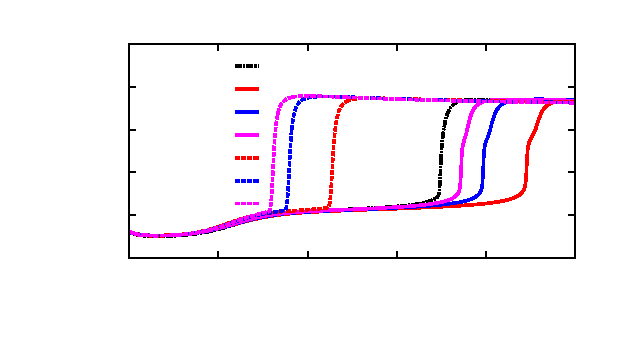
\includegraphics{ch-dynamics/T_32}}%
    \gplfronttext
  \end{picture}%
\endgroup
}
  \resizebox{0.8\textwidth}{!}{% GNUPLOT: LaTeX picture with Postscript
\begingroup
  \makeatletter
  \providecommand\color[2][]{%
    \GenericError{(gnuplot) \space\space\space\@spaces}{%
      Package color not loaded in conjunction with
      terminal option `colourtext'%
    }{See the gnuplot documentation for explanation.%
    }{Either use 'blacktext' in gnuplot or load the package
      color.sty in LaTeX.}%
    \renewcommand\color[2][]{}%
  }%
  \providecommand\includegraphics[2][]{%
    \GenericError{(gnuplot) \space\space\space\@spaces}{%
      Package graphicx or graphics not loaded%
    }{See the gnuplot documentation for explanation.%
    }{The gnuplot epslatex terminal needs graphicx.sty or graphics.sty.}%
    \renewcommand\includegraphics[2][]{}%
  }%
  \providecommand\rotatebox[2]{#2}%
  \@ifundefined{ifGPcolor}{%
    \newif\ifGPcolor
    \GPcolortrue
  }{}%
  \@ifundefined{ifGPblacktext}{%
    \newif\ifGPblacktext
    \GPblacktexttrue
  }{}%
  % define a \g@addto@macro without @ in the name:
  \let\gplgaddtomacro\g@addto@macro
  % define empty templates for all commands taking text:
  \gdef\gplbacktext{}%
  \gdef\gplfronttext{}%
  \makeatother
  \ifGPblacktext
    % no textcolor at all
    \def\colorrgb#1{}%
    \def\colorgray#1{}%
  \else
    % gray or color?
    \ifGPcolor
      \def\colorrgb#1{\color[rgb]{#1}}%
      \def\colorgray#1{\color[gray]{#1}}%
      \expandafter\def\csname LTw\endcsname{\color{white}}%
      \expandafter\def\csname LTb\endcsname{\color{black}}%
      \expandafter\def\csname LTa\endcsname{\color{black}}%
      \expandafter\def\csname LT0\endcsname{\color[rgb]{1,0,0}}%
      \expandafter\def\csname LT1\endcsname{\color[rgb]{0,1,0}}%
      \expandafter\def\csname LT2\endcsname{\color[rgb]{0,0,1}}%
      \expandafter\def\csname LT3\endcsname{\color[rgb]{1,0,1}}%
      \expandafter\def\csname LT4\endcsname{\color[rgb]{0,1,1}}%
      \expandafter\def\csname LT5\endcsname{\color[rgb]{1,1,0}}%
      \expandafter\def\csname LT6\endcsname{\color[rgb]{0,0,0}}%
      \expandafter\def\csname LT7\endcsname{\color[rgb]{1,0.3,0}}%
      \expandafter\def\csname LT8\endcsname{\color[rgb]{0.5,0.5,0.5}}%
    \else
      % gray
      \def\colorrgb#1{\color{black}}%
      \def\colorgray#1{\color[gray]{#1}}%
      \expandafter\def\csname LTw\endcsname{\color{white}}%
      \expandafter\def\csname LTb\endcsname{\color{black}}%
      \expandafter\def\csname LTa\endcsname{\color{black}}%
      \expandafter\def\csname LT0\endcsname{\color{black}}%
      \expandafter\def\csname LT1\endcsname{\color{black}}%
      \expandafter\def\csname LT2\endcsname{\color{black}}%
      \expandafter\def\csname LT3\endcsname{\color{black}}%
      \expandafter\def\csname LT4\endcsname{\color{black}}%
      \expandafter\def\csname LT5\endcsname{\color{black}}%
      \expandafter\def\csname LT6\endcsname{\color{black}}%
      \expandafter\def\csname LT7\endcsname{\color{black}}%
      \expandafter\def\csname LT8\endcsname{\color{black}}%
    \fi
  \fi
  \setlength{\unitlength}{0.0500bp}%
  \begin{picture}(5760.00,3024.00)%
    \gplgaddtomacro\gplbacktext{%
      \csname LTb\endcsname%
      \put(948,704){\makebox(0,0)[r]{\strut{}0.0e+00}}%
      \put(948,1115){\makebox(0,0)[r]{\strut{}7.0e-04}}%
      \put(948,1526){\makebox(0,0)[r]{\strut{}1.4e-03}}%
      \put(948,1937){\makebox(0,0)[r]{\strut{}2.1e-03}}%
      \put(948,2348){\makebox(0,0)[r]{\strut{}2.8e-03}}%
      \put(948,2759){\makebox(0,0)[r]{\strut{}3.5e-03}}%
      \put(1080,484){\makebox(0,0){\strut{} 0}}%
      \put(1937,484){\makebox(0,0){\strut{} 1}}%
      \put(2793,484){\makebox(0,0){\strut{} 2}}%
      \put(3650,484){\makebox(0,0){\strut{} 3}}%
      \put(4506,484){\makebox(0,0){\strut{} 4}}%
      \put(5363,484){\makebox(0,0){\strut{} 5}}%
      \put(-218,1731){\rotatebox{-270}{\makebox(0,0){\strut{}\vspace{-28pt}$Y_{\rm CH_3OCH_2O_2}$}}}%
      \put(3221,154){\makebox(0,0){\strut{}$x/D$}}%
    }%
    \gplgaddtomacro\gplfronttext{%
      \csname LTb\endcsname%
      \put(4707,2473){\makebox(0,0)[r]{\strut{}Steady 3.2 m/s}}%
      \csname LTb\endcsname%
      \put(4707,2253){\makebox(0,0)[r]{\strut{}100 Hz DV}}%
      \csname LTb\endcsname%
      \put(4707,2033){\makebox(0,0)[r]{\strut{}50 Hz DV}}%
      \csname LTb\endcsname%
      \put(4707,1813){\makebox(0,0)[r]{\strut{}25 Hz DV}}%
      \csname LTb\endcsname%
      \put(4707,1593){\makebox(0,0)[r]{\strut{}100 Hz IV}}%
      \csname LTb\endcsname%
      \put(4707,1373){\makebox(0,0)[r]{\strut{}50 Hz IV}}%
      \csname LTb\endcsname%
      \put(4707,1153){\makebox(0,0)[r]{\strut{}25 Hz IV}}%
    }%
    \gplbacktext
    \put(0,0){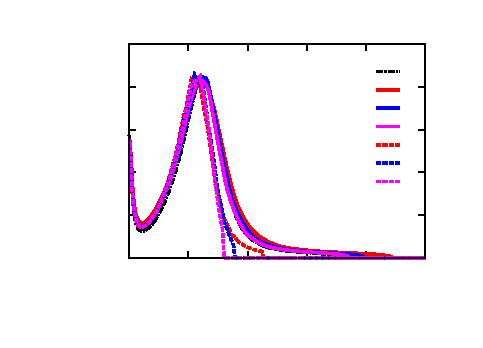
\includegraphics{RO2_32}}%
    \gplfronttext
  \end{picture}%
\endgroup
}
  \resizebox{0.8\textwidth}{!}{% GNUPLOT: LaTeX picture with Postscript
\begingroup
  \makeatletter
  \providecommand\color[2][]{%
    \GenericError{(gnuplot) \space\space\space\@spaces}{%
      Package color not loaded in conjunction with
      terminal option `colourtext'%
    }{See the gnuplot documentation for explanation.%
    }{Either use 'blacktext' in gnuplot or load the package
      color.sty in LaTeX.}%
    \renewcommand\color[2][]{}%
  }%
  \providecommand\includegraphics[2][]{%
    \GenericError{(gnuplot) \space\space\space\@spaces}{%
      Package graphicx or graphics not loaded%
    }{See the gnuplot documentation for explanation.%
    }{The gnuplot epslatex terminal needs graphicx.sty or graphics.sty.}%
    \renewcommand\includegraphics[2][]{}%
  }%
  \providecommand\rotatebox[2]{#2}%
  \@ifundefined{ifGPcolor}{%
    \newif\ifGPcolor
    \GPcolortrue
  }{}%
  \@ifundefined{ifGPblacktext}{%
    \newif\ifGPblacktext
    \GPblacktexttrue
  }{}%
  % define a \g@addto@macro without @ in the name:
  \let\gplgaddtomacro\g@addto@macro
  % define empty templates for all commands taking text:
  \gdef\gplbacktext{}%
  \gdef\gplfronttext{}%
  \makeatother
  \ifGPblacktext
    % no textcolor at all
    \def\colorrgb#1{}%
    \def\colorgray#1{}%
  \else
    % gray or color?
    \ifGPcolor
      \def\colorrgb#1{\color[rgb]{#1}}%
      \def\colorgray#1{\color[gray]{#1}}%
      \expandafter\def\csname LTw\endcsname{\color{white}}%
      \expandafter\def\csname LTb\endcsname{\color{black}}%
      \expandafter\def\csname LTa\endcsname{\color{black}}%
      \expandafter\def\csname LT0\endcsname{\color[rgb]{1,0,0}}%
      \expandafter\def\csname LT1\endcsname{\color[rgb]{0,1,0}}%
      \expandafter\def\csname LT2\endcsname{\color[rgb]{0,0,1}}%
      \expandafter\def\csname LT3\endcsname{\color[rgb]{1,0,1}}%
      \expandafter\def\csname LT4\endcsname{\color[rgb]{0,1,1}}%
      \expandafter\def\csname LT5\endcsname{\color[rgb]{1,1,0}}%
      \expandafter\def\csname LT6\endcsname{\color[rgb]{0,0,0}}%
      \expandafter\def\csname LT7\endcsname{\color[rgb]{1,0.3,0}}%
      \expandafter\def\csname LT8\endcsname{\color[rgb]{0.5,0.5,0.5}}%
    \else
      % gray
      \def\colorrgb#1{\color{black}}%
      \def\colorgray#1{\color[gray]{#1}}%
      \expandafter\def\csname LTw\endcsname{\color{white}}%
      \expandafter\def\csname LTb\endcsname{\color{black}}%
      \expandafter\def\csname LTa\endcsname{\color{black}}%
      \expandafter\def\csname LT0\endcsname{\color{black}}%
      \expandafter\def\csname LT1\endcsname{\color{black}}%
      \expandafter\def\csname LT2\endcsname{\color{black}}%
      \expandafter\def\csname LT3\endcsname{\color{black}}%
      \expandafter\def\csname LT4\endcsname{\color{black}}%
      \expandafter\def\csname LT5\endcsname{\color{black}}%
      \expandafter\def\csname LT6\endcsname{\color{black}}%
      \expandafter\def\csname LT7\endcsname{\color{black}}%
      \expandafter\def\csname LT8\endcsname{\color{black}}%
    \fi
  \fi
  \setlength{\unitlength}{0.0500bp}%
  \begin{picture}(4320.00,3024.00)%
    \gplgaddtomacro\gplbacktext{%
      \csname LTb\endcsname%
      \put(948,704){\makebox(0,0)[r]{\strut{}0.0e+00}}%
      \put(948,1115){\makebox(0,0)[r]{\strut{}6.0e-03}}%
      \put(948,1526){\makebox(0,0)[r]{\strut{}1.2e-02}}%
      \put(948,1937){\makebox(0,0)[r]{\strut{}1.8e-02}}%
      \put(948,2348){\makebox(0,0)[r]{\strut{}2.4e-02}}%
      \put(948,2759){\makebox(0,0)[r]{\strut{}3.0e-02}}%
      \put(1080,484){\makebox(0,0){\strut{} 0}}%
      \put(1649,484){\makebox(0,0){\strut{} 1}}%
      \put(2217,484){\makebox(0,0){\strut{} 2}}%
      \put(2786,484){\makebox(0,0){\strut{} 3}}%
      \put(3354,484){\makebox(0,0){\strut{} 4}}%
      \put(3923,484){\makebox(0,0){\strut{} 5}}%
      \put(-218,1731){\rotatebox{-270}{\makebox(0,0){\strut{}\vspace{-28pt}$Y_{\rm H_2O_2}$}}}%
      \put(2501,154){\makebox(0,0){\strut{}$x/D$}}%
    }%
    \gplgaddtomacro\gplfronttext{%
      \csname LTb\endcsname%
      \put(1960,2603){\makebox(0,0)[r]{\strut{}Steady 3.2 m/s}}%
      \csname LTb\endcsname%
      \put(1960,2427){\makebox(0,0)[r]{\strut{}100 Hz DV}}%
      \csname LTb\endcsname%
      \put(1960,2251){\makebox(0,0)[r]{\strut{}50 Hz DV}}%
      \csname LTb\endcsname%
      \put(1960,2075){\makebox(0,0)[r]{\strut{}25 Hz DV}}%
      \csname LTb\endcsname%
      \put(1960,1899){\makebox(0,0)[r]{\strut{}100 Hz IV}}%
      \csname LTb\endcsname%
      \put(1960,1723){\makebox(0,0)[r]{\strut{}50 Hz IV}}%
      \csname LTb\endcsname%
      \put(1960,1547){\makebox(0,0)[r]{\strut{}25 Hz IV}}%
    }%
    \gplbacktext
    \put(0,0){\includegraphics{H2O2_32}}%
    \gplfronttext
  \end{picture}%
\endgroup
}
  \normalsize
  \caption{Temperature, methyoxymethylperoxy radical, and hydrogen peroxide mass fraction profiles along the $Z = 0.24$ iso-contour at $3.2$ m/s.  DV: decreasing-velocity, and IV: increasing-velocity.}
  \label{fig:ind_frq}
\end{figure}

\section{Summary}

In this chapter, the two-dimensional nonpremixed DME flames in heated air coflows were investigated computationally due to the difficulty in well-controlled experiments otherwise.  The understanding of the low-temperature chemistry obtained in the one-dimensional counterflow configuration presented in Chapter~\ref{ch:NTC} is benefical to elucidate the importance of low-temperature chemistry in flame dynamics at elevated temperatures and pressures.  In the steady cases, besides the kinematic stabilization mechanism that balances the traditional tribrachial flame propagation in coflows at nonautoignitive conditions, the kinetic stabilization mechanism induced by autoignition can also be important under certain conditions.  Since low-temperature chemistry dictates the first-stage autoignition delay time and the subsequent heat release, it affects the morphology of the multibrachial structure of the autoignition front.  With advanced computational diagnostics, the thermal and chemical structures as well as the donimant stablization mechanisms were elucidated for steady cases at various boundary conditions.  A regime diagram was proposed to generalize the stablization mechanism.  

Furthermore, realizing that one of the major characteristics of practical engine conditions is unsteadiness, flame dynamics in the same configuration were investigated by forcing harmonic oscillations between two steady cases at different oscillation frequencies.  The transition in the combustion mode during the oscillation was observed and quantified.  Finally, the coupling effects of low-temperature chemistry, high-temperature chemistry, and transport were elucidated.  Such understanding could be benefical to future turbulent studies.

\chapter{Sooting Limits of Laminar Stagnation-Flow Flames}\label{ch:biofuel}

Soot emission control is an important research area in combustion.  As reviewed in Chapter~\ref{sec:intro-biofuel}, the fundamental understanding of the chemical kinetics in sooting flames is still under development.  Although oxygenated additives have been found to reduce particular matter emissions~\cite{graboski98}, the precise role of oxygenated additives on soot emission reduction has not yet come to a scientific consensus.  Moreover, since soot formation is a kinetically controlled process~\cite{vandsburger85}, the finite residence time effect also needs to be considered.  Therefore, the experimental and computational investigation of sooting limits of three neat liquid diesel/biofuel components, specifically, $n$-heptane, $n$-butanol, and methyl butanoate, in a nonpremixed stagnation-flow is presented in this chapter.  A combined chemical kinetic model with detailed polycyclic aromatic hydrocarbon (PAH) chemistry is constructed to investigate the important pathways of soot formation with these three fuels.

This choice of the target fuels is motivated by both practical and scientific concerns. First, butanol has more diverse non-food sources of supply than ethanol, which has been derived primarily from corn. Second, methyl butanoate is chosen not only because it is a typical biodiesel surrogate but also due to the availability of detailed chemical kinetic models. Third and most important, the boiling points of $n$-butanol and methyl butanoate are $391$ K and $375$ K, respectively, which are very close to that of $n$-heptane ($372$ K). This similarity in the vaporization characteristics enables similar fuel vapor concentrations and assures similar rates of supply of the vaporized fuel to the flame region.

\section{Experimental Methodology}\label{sec:biofuel-exp}

The sooting limits of nonpremixed model diesel/biofuel components, in terms of the critical strain rate (CSR) at which soot inception starts to happen when the residence time, which is the inverse of the strain rate, is further increased, were measured at atmospheric pressure in a liquid pool stagnation-flow configuration. An unheated oxidizer stream impinged against the liquid fuel pool, and flames were established by spark ignition. Coflowing nitrogen was utilized as the shielding gas to minimize the disturbance from the surroundings.  With the $20$ mm nozzle and pool diameter, the separation distance between the oxidizer nozzle and liquid pool was maintained at $13$ mm to assure a well-characterized stagnation flow and also to enable better measurement of the velocity field by Laser Doppler Velocimetry (LDV).  The schematic of the liquid pool stagnation-flow apparatus is shown in Fig.~\ref{fig:setup}, and details about the auxiliary system can be found elsewhere~\cite{liu10}.

Due to the oxygen content in $n$-butanol and methyl butanoate, their flame temperatures are lower than $n$-heptane. Since soot formation is highly sensitive to temperature~\cite{wang11}, this thermal effect has to be eliminated to elucidate the chemical effects. In the present study, $n$-butanol and methyl butanoate flame temperatures were increased to be the same as $n$-heptane by replacing a portion of the nitrogen in the oxidizer stream with argon, which is the same approach taken by Axelbaum, Law, and co-workers~\cite{du89,du91,axelbaum91}. The amount of nitrogen replacement was calculated with CHEMKIN's equilibrium solver EQUIL~\cite{chemkin} for stoichiometric fuel/oxidizer mixtures, and the diluent concentrations are summarized in Table.~\ref{table:exp_condition}.  Although the replacement was calculated based on premixed stoichiometric mixtures, the thermal environment of all three fuels cases under the same strain rate and oxygen mole fraction in the stagnation-flow configuration is nearly the same, according to the simulations, which will be discussed in detail in Sec.~\ref{sec:biofuel-results}.  Liquid $n$-heptane, $n$-butanol, and methyl butanoate were fed to the liquid pool by a syringe pump at room temperature.

\begin{figure}[t]
  \centering
  \scriptsize
  \includegraphics[width=0.8\textwidth]{ch-biofuel/Setup.png}
  \normalsize
  \caption{Schematic of the liquid pool stagnation-flow apparatus~\cite{liu10}.  The heating system was not activated in the current study.}
  \label{fig:setup}
\end{figure}

\begin{table*}
  \caption{Oxidizer stream composition in mole fractions to maintain the same adiabatic flame temperature of the three fuels with the same oxygen concentration in the oxidizer stream.}
  \label{table:exp_condition}
  \centering
  \resizebox{1.0\textwidth}{!}{
  \begin{tabular}{ll*{8}{c}}
    \hline
     & \multicolumn{8}{c}{$O_2$} \\
    \cline{3-10}
     &  & $0.2000$ & $0.2025$ & $0.2050$ & $0.2075$ & $0.2100$ & $0.2150$ & $0.2200$ & $0.2250$ \\
    \hline
    $n-C_4H_9OH$ & $N_2$ & $0.7640$ & $0.7600$ & $0.7560$ & $0.7521$ \\
                 & $Ar$ & $0.0360$ & $0.0375$ & $0.0390$ & $0.0404$ \\
    $C_5H_{10}O_2$ & $N_2$ & & & $0.7119$ & & $0.7017$ & $0.6915$ & $0.6811$ & $0.6707$ \\
                 & $Ar$ & & & $0.0831$ & & $0.0883$ & $0.0935$ & $0.0989$ & $0.1043$ \\ 
    \hline
  \end{tabular}
}
\end{table*}


Soot detection was based on luminosity observations with a Nikon D700 camera, for Du \emph{et al.}~\cite{du89} found that such measurements agreed well with light scattering detection and were a convenient indicator of the presence of soot particles. The experimental procedure to identify the sooting limit is briefly summarized here. First, the oxidizer component flow rates were set, and a non-sooting blue flame was established. Then, the bypass valve placed upstream of the oxidizer nozzle was slowly adjusted to divert oxidizer out of the system, effectively reducing the velocity of the stream and, consequently, the strain rate. The residence time was further increased until yellow luminosity began to appear on the fuel rich side of the flame. A standard single-component LDV measurement was performed along the axial centerline under this threshold flow condition, and the local strain rate was determined as the axial velocity gradient upstream of the flame~\cite{du89}. Following this procedure, the sooting limits for the three fuels with different oxygen concentrations in the oxidizer streams were identified.  Although this luminosity measurement was not quantified, the CSR measurements were found to be repeatable.

\section{Computational Methodology}

The liquid pool stagnation-flow flames were simulated with the FlameMaster code~\cite{flamemaster}, including detailed PAH chemistry and a detailed soot model. The boundary conditions on the fuel side were specified following Bui-Pham \emph{et al.}~\cite{buipham91}. In brief, the Antoine equation~\cite{polingbook} was used to close the boundary value problem by relating the liquid pool surface temperature and vapor pressure, yielding a relationship for the fuel mole fraction at the surface. As in the experiment, the local strain rate was determined as the gradient of the velocity profile on the oxidizer side, ahead of the flame. 

Furthermore, since the luminosity observations cannot be simulated directly, the computational CSRs were determined based on an alternative metric, and a critical value of this metric was chosen to match the experimental results of $n$-heptane at larger $X_{O_2}$ cases and was kept fixed for all other cases.  The global domain-integrated soot volume fraction ($f_V$), the temperature-weighted global domain-integrated soot volume fraction ($f_V*$T$^4$), and the maxima of the corresponding single-point values were considered as potential metrics.  However, the qualitative trends presented in the next section were found to be insensitive to the choice of the threshold value or determination metrics that were explored.  Therefore, the global domain-integrated $f_V$ (m$^3$/m$^2$) were chosen as the metric for computational determination of CSRs in the following sections.

\subsection{Chemical Model} 

A detailed chemical model including PAH chemistry was constructed from three well validated models corresponding to the fuels of interest. A mechanism with PAH chemistry of engine relevant fuels was developed by Blanquart, Pitsch, and co-workers~\cite{blanquart09b,narayanaswamy10}. This mechanism has been validated extensively against experimental measurements of ignition delay times, laminar burning velocities, and species profiles in both premixed and nonpremixed flames over a large range of equivalence ratios and pressures for small hydrocarbons, C$_3$ and C$_4$ species, (substituted) aromatics, $n$-heptane, and iso-octane. Of particular interest to this work, the mechanism was validated in $n$-heptane nonpremixed flames against the measurements of Berta \emph{et al.}~\cite{berta06}.  This mechanism was adopted as the base mechanism with PAH chemistry. Reduced oxidation/pyrolysis chemistry of $n$-butanol and methyl butanoate kinetic models was adopted from Liu \emph{et al.}~\cite{liu11} and combined with the base mechanism.  These models were reduced from the detailed mechanisms of Sarathy \emph{et al.}~\cite{sarathy09} and Ga\"il \emph{et al.}~\cite{gail08}, respectively. Details about the mechanism reduction, validation, and reduced mechanisms can be found in Liu \emph{et al.}~\cite{liu11}.  All the common reactions among the base mechanism and the addtional mechanisms were retained from the base mechanism to maintain compatibility with the PAH mechanism. The thermal and transport data of the species that appeared only in the $n$-butanol and methyl butanoate mechanism were taken from these latter works, and species in common were taken from the base mechanism. The combined mechanism consists of $220$ species and $2259$ forward and backward reactions; none of the reaction rate parameters were adjusted in the combined mechanism.

\begin{figure}[t]
  \centering
  \scriptsize
  \includegraphics[width=1.0\textwidth]{ch-biofuel/NB.png}
  \normalsize
  \caption{Mechanism validation of $n$-butanol laminar flame speeds, against the experimental (symbols) and computational (dotted lines) results from Liu \emph{et al.}~\cite{liu11}. $P=1$ atm and $T=353$ K.}
  \label{fig:validation_NB}
\end{figure}

The combined mechanism  was validated against laminar flame speed measurements~\cite{liu11} and compared with the predictions by the original mechanisms; results of this validation are shown in Figs.~\ref{fig:validation_NB} and~\ref{fig:validation_MB}.  As no difference was found between the validation results calculated by the combined and the original $n$-heptane mechanism, $n$-heptane laminar speed validation is not included and can be found in the referenced works~\cite{blanquart09b,narayanaswamy10}.  The differences between the combined mechanism and the original mechanism for $n$-butanol and methyl butanoate are attributed to the differences in the base chemistry, with the combined mechanism generally giving improved agreement with the experimental measurements.  

\begin{figure}[t]
  \centering
  \scriptsize
  \includegraphics[width=1.0\textwidth]{ch-biofuel/MB.png}
  \normalsize
  \caption{Mechanism validation of methyl butanoate laminar flame speeds, against the experimental (symbols) and computational (dotted lines) results from Liu \emph{et al.}~\cite{liu11}. $P=1$ atm and $T=353$ K.}
  \label{fig:validation_MB}
\end{figure}

In addition, the combined mechanism was further validated against extinction strain rate (ESR) measurements in the nonpremixed liquid pool stagnation-flow system, as shown in Figs.~\ref{fig:validation-ESR_NH} to~\ref{fig:validation-ESR_MB}.  The computational ESRs for $n$-heptane and methyl butanoate were compared with the experimental studies of Seshadri and co-workers~\cite{seshadri08,niemann10}, and details about the experimental procedure and conditions can be found therein.  These measurements were augmented with our own measurements of ESR for $n$-butanol with the same apparatus presented in the previous section.  The same experimental procedure as Seshadri and co-workers was adopted, except that the ESR was defined by the local strain rate rather than the global one, the former being the fundamentally more relevant quantity.  In all cases, the experimental measurements and simulation results were compared based on the same definition of the strain rate.  However, as demonstrated in Liu \emph{et al.}~\cite{liu11b}, deteminations based on a given definition are consistent.  As shown in Figs.~\ref{fig:validation-ESR_NH} to~\ref{fig:validation-ESR_MB}, computational ESRs for $n$-heptane and methyl butanoate agree well with the experimental measurements and are slightly overpredicted for $n$-butanol.  

\begin{figure}[t]
  \centering
  \scriptsize
  \includegraphics[width=1.0\textwidth]{ch-biofuel/NH-ESR.png}
  \normalsize
  \caption{Mechanism validation for $n$-heptane against the extinction strain rates measurements in nonpremixed stagnation-flow systems.}
  \label{fig:validation-ESR_NH}
\end{figure}


\begin{figure}[t]
  \centering
  \scriptsize
  \includegraphics[width=1.0\textwidth]{ch-biofuel/NB-ESR.png}
  \normalsize
  \caption{Mechanism validation for $n$-butanol against the extinction strain rates measurements in nonpremixed stagnation-flow systems.}
  \label{fig:validation-ESR_NB}
\end{figure}

\begin{figure}[t]
  \centering
  \scriptsize
  \includegraphics[width=1.0\textwidth]{ch-biofuel/MB-ESR.png}
  \normalsize
  \caption{Mechanism validation for methyl butanoate against the extinction strain rates measurements in nonpremixed stagnation-flow systems.}
  \label{fig:validation-ESR_MB}
\end{figure}

\subsection{Soot Model}\label{sec:biofuel-soot_model}

Far too many soot particles are present to track individually, so the population is described statistically with Number Density Function (NDF), $N_i$.  The NDF describes the size distribution of soot particles and is typically bimodal~\cite{zhao05}.  Due to persistent nucleation of soot particles from PAH, one mode of the NDF contains the smaller incipient spherical soot particles.  The other mode contains larger and more mature fractal aggregates formed from coagulation of smaller spherical primary particles.  A two-dimensional internal coordinate is used to define the NDF: the volume $V$ and the surface area $S$.  The transport equation governing the evolution of NDF is very high-dimensional (three spatial dimensions and two internal dimensions).  Therefore, the only tractable model is the Method of Moments, in which moments of the NDF are solved for rather than the NDF itself.  The moments of the NDF $M_{x,y}$ are given by
\begin{equation}\label{eq:defM}
M_{x,y} = \sum_{i} V_i^x S_i^y N_i,
\end{equation}
where summation over all particle sizes is performed.  Although the distribution of soot particle sizes is not provided directly with the Method of Moments, quantities that are of interest in engineering applications, such as the soot volume fraction, total number density, average primary particle diameter, etc., are well captured.  

The evolution of the NDF is described by the Population Balance Equation (PBE)~\cite{friedlander00}.  Similarly, the transport equation for the evolution of the moments of NDF can be obtained by taking the moments of the PBE, that is, 
\begin{equation}\label{eq:M}
\pp{M_{x,y}}{t} + \pp{u_iM_{x,y}}{x_i} = \pp{}{x_i}\left(0.55 \frac{\nu}{T} \pp{T}{x_i} M_{x,y}\right) + \dot{M}_{x,y}\;,
\end{equation}
where the first term on the right hand side is the thermophoresis of soot particles\cite{waldmann66} and molecular diffusion is neglected~\cite{bisetti12}.  Subsequently, this term is combined with the convective term, and the total velocity is denoted by
\begin{equation}\label{eq:therm}
  u_i^\ast = u_i - 0.55 \frac{\nu}{T} \pp{T}{x_i}\;.
\end{equation}
The source term in Eq.~\ref{eq:M} contains incipient soot particle nucleation from PAH dimers~\cite{schuetz02,wong09,blanquart09c}, PAH condensation~\cite{park03,mitchell98,mitchell03}, particle coagulation~\cite{mueller09b}, surface growth by the HACA mechanism~\cite{frenklach91}, oxidation~\cite{kazakov95,neoh81}, and oxidation-induced fragmentation~\cite{mueller11a}.  

The major challenge with the Method of Moments is the closure problem, which is the fact that the source terms for the moment equations depend on moments which are not solved for.  In this disseration, closure is achieved with the Hybrid Method of Moments (HMOM) developed by Mueller \emph{et al.}~\cite{mueller09a,mueller09b,mueller11a}, and the details of the above models can be found in those works.  Briefly, in HMOM, the contribution from the smaller incipient particles to the moments is described with a delta function as in the Direct Quadrature Method of Moments (DQMOM)~\cite{marchisio05}.  Moreover, the contribution to the moments from the larger particles is described with polynomial interpolation as in the Method of Moments with Interpolative Closure (MOMIC)~\cite{frenklach87}.  Therefore, an arbitrary moment is given by
\begin{equation}\label{eq:hmom}
  M_{x,y} = V_0^x S_0^y N_0 + \exp{\sum_{r=0}^R{\sum_{k=0}^r{a_{r,k}x^ky^{r-k}}}}\;,
\end{equation}
where the location of the delta function ($V_0,S_0$) is fixed and $R$ is the order of the polynomial interpolation.  A transport equation is solved for the weight of the delta function $N_0$.  The transport equation for this quantity is the same as Eq.~\ref{eq:M} with the source term given by
\begin{equation}\label{eq:N0}
  \dot{N}_0 = \lim_{\alpha,\beta\rightarrow\infty}{\frac{\dot{M}_{-\alpha,-\beta}}{V_0^{-\alpha}S_0^{-\beta}}}\;.
\end{equation}
Given the weight of the delta function $N_0$, the polynomial interpolation coefficients are obtained from a set of moments which are solved for.  In this work, $R=1$, so three moment equations are solved other than $N_0$: the total number density $M_{0,0}$, the total soot volume $M_{1,0}$, and the total soot surface area $M_{0,1}$.  Further details about HMOM and the soot model can be found in Mueller \emph{et al.}~\cite{mueller09a,mueller09b,mueller11a} and the references therein.

\section{Results: Sooting Limits}
\label{sec:biofuel-results}

As mentioned in Sec.~\ref{sec:biofuel-exp}, argon dilution was used to keep the thermal environment of the three fuel cases nearly the same.  This is justified with the simulation results of the temperature profiles for three fuel cases under the same strain rate and oxygen mole fraction, as shown in Fig.~\ref{fig:thermal}.  The difference among the peak temperatures is less than $20$ K, and the peak locations differ by less than $0.1$ mm.  Furthermore, on the fuel-rich side, in the vicinity where soot is formed, the maximum temperature difference among the fuels is less than $\pm20$ K.  Also, simulation results show that the liquid surface temperatures for all three fuels stay about $20$ K below their respective boiling points, and the liquid surface temperatures are nearly constant (within $0.3\%$), regardless of the change in oxygen mole fractions.  Consequently, the thermal environment is maintained nearly the same for all three fuels, and chemical effects have therefore been isolated from thermal effects. 

The critical strain rates (CSRs) corresponding to the sooting limits from the experiments and computations are shown in Fig.~\ref{fig:Exp-Comp}. For each set of data, the region above/left of the data corresponds to non-sooting flames, and the region below/right of the data corresponds to sooting flames. For all three fuels, the CSR increases with increasing oxygen concentration in the oxidizer stream, which has been previously characterized as a thermal effect~\cite{du91}. In addition, both experiment and computation show that methyl butanoate has substantially lower CSRs compared to  $n$-heptane and $n$-butanol. 

This distinct trend warrants further investigation.  Noting that, the CSRs are defined (experimentally and computationally) based on an absolute amount of soot, the fact that the CSRs are substantially lower for methyl butanoate compared to the other two fuels could then be due to either or both of the following hypotheses.  First, less soot is formed from methyl butanoate overall, regardless of strain rate.  Second, the chemical pathways leading to PAH and soot formation for methyl butanoate are slower and are more strongly suppressed with decreasing residence time (increasing strain rate).  The relative roles of these two hypotheses require further analysis.

\begin{figure}[t]
  \centering
  \scriptsize
  \vspace{-0.1in}
  \includegraphics[width=1.0\textwidth]{ch-biofuel/Thermal.png}
  \normalsize
  \caption{Temperature (solid line) and $f_V$ (dash-dotted line) profiles at the strain rate of $16$ s$^{-1}$ and $X_{O_2}=0.2$.}
  \label{fig:thermal}
\end{figure}

\begin{figure}[t]
  \centering
  \scriptsize
  \vspace{0.5in}
  \includegraphics[width=1.0\textwidth]{ch-biofuel/Exp-Comp.png}
  \normalsize
  \caption{Experimental (symbols) and computational (lines) CSRs.}
  \label{fig:Exp-Comp}
\end{figure}

\begin{figure}[t]
  \centering
  \scriptsize
  \vspace{-0.1in}
  \includegraphics[width=1.0\textwidth]{ch-biofuel/SV-SR.png}
  \normalsize
%  \vspace{-0.1in}
  \caption{The responses of the integrated $f_V$ to strain rate at $X_{O_2}=0.2$.}
  \label{fig:fv}
\end{figure}

\section{Mechanistic Analysis}

To elucidate the role of the above two hypotheses, mechanistic analysis was conducted for all three fuels to investigate the response of soot volume fraction to strain rate, chemical pathways for PAH formation, and the rate-limiting steps for PAH formation for each of the three fuels.

\subsection{Volume Fraction Response to Strain Rate}

The integrated $f_V$ under various strain rates are shown in Fig.~\ref{fig:fv}.  For all three fuels, as the strain rate increases, less soot is formed due to reduced residence time.  At all strain rates, $n$-butanol is overall as sooty as $n$-heptane, while methyl butanoate is the least sooty.  If a critical $f_V$ is chosen and a horizontal line drawn based on this choice, the intersections of the horizontal line and the three $f_V$ profiles give the corresponding CSRs for the three fuels.  This is indeed how the computational CSRs were determined in the current study.  Therefore, the CSRs correlate with the total amount of soot formed, explaining at least in part the CSR trends. However, detailed chemical pathway analysis is still needed to elucidate the differences in the global sooting behavior as well as to see if there are any significant differences in PAH pathways with different timescales for the three fuels that could further explain the observed trends in CSRs.

\subsection{Sensitivity and Reaction Pathway Analysis}

\begin{figure}[t]
  \centering
  \scriptsize
  \includegraphics[trim=0mm 0mm 0mm 8mm, clip=true,width=1.0\textwidth]{ch-biofuel/Chain.png}
  \includegraphics[trim=0mm 0mm 0mm 8mm, clip=true,width=1.0\textwidth]{ch-biofuel/Ring.png}
  \normalsize
%  \vspace{-0.2in}
  \caption{Sensitivity of the maximum naphthalene mass fraction to kinetics at the strain rate of $16$ s$^{-1}$ and $X_{O_2}=0.2$. Top: Intermediate chain radical reactions. Bottom: Ring formation reactions.}
  \label{fig:SA4}
\end{figure}

To understand the distinct differences in PAH evolution between the three fuels, sensitivity and reaction path analysis were performed for a representative PAH species, naphthalene (C$_{10}$H$_8$).  As shown in Fig.~\ref{fig:SA4} and Fig.~\ref{fig:Pathways_PAH}, naphthalene shows roughly the same sensitivities to the same reactions for each of the fuels, and the chemical pathways of naphthalene are essentially the same after the fuel cracking. Initially, fuel cracks to unsaturated C$_3$ to C$_5$ chains through H abstraction followed by $\beta$-scission reactions. These smaller molecules further decompose into allyl radicals (CH$_2$=CH-CH$_2^*$ or A-C$_3$H$_5$) and propene (C$_3$H$_6$), which contribute to C$_5$ and C$_6$ ring formation by either combining with acetylene (C$_2$H$_2$) or forming propargyl (C$_3$H$_3$), the latter further combining with itself to form aromatic rings. Larger species (predominantly toluene and indene) are formed by the combination of benzene and cyclopentadiene with smaller species, such as CH$_3$, C$_2$H$_2$, and C$_3$H$_3$. Two pathways directly contribute to naphthalene formation, namely, cyclopentadienyl (C$_5$H$_5$) radical recombination and methyl addition to indenyl (C$_9$H$_7$)
\begin{align*}
  2 {\rm C}_5{\rm H}_5 &\longrightarrow {\rm C}_{10}{\rm H}_8 + 2 {\rm H}\\
  {\rm C}_9{\rm H}_7 + {\rm C}{\rm H}_3 &\longrightarrow {\rm C}_{10}{\rm H}_8 + 2 {\rm H}.
\end{align*}

\begin{figure*}[t]
  \centering
  \scriptsize
  \includegraphics[width=1.0\textwidth]{ch-biofuel/Pathways-PAH.png}
  \normalsize
  \caption{Chemical pathways for naphthalene formation at the strain rate of $16$ s$^{-1}$ and $X_{O_2}=0.2$.}
  \label{fig:Pathways_PAH}
\end{figure*}

\begin{figure*}[t]
  \centering
  \scriptsize
  \includegraphics[width=1.0\textwidth]{ch-biofuel/Pathways_Fuel.png}
  \normalsize
  \caption{Fuel specific pathways for C$_3$H$_6$ and A-C$_3$H$_5$ formation at the strain rate of $16$ s$^{-1}$ and $X_{O_2}=0.2$. From left to right: $n$-heptane, $n$-butanol, and methyl butanoate.  The numbers indicate the relative contribution (in percentages) to the formation of the ``downstream'' species.}
  \label{fig:Pathways_Fuel}
\end{figure*}

Although the PAH pathways for the three fuels are similar, the formation of these soot precursors from the fuel cracking processes and the relative importance of the subsequent chemical pathways of PAH growth are fuel specific. Noting the similarity in the chemical pathways beyond A-C$_3$H$_5$ and C$_3$H$_6$, the fuel specific breakdown pathways that lead to the generation of these precursors are depicted in Fig.~\ref{fig:Pathways_Fuel}. For both $n$-heptane and $n$-butanol, 1-butene (P-C$_4$H$_8$) is a product of the fuel decomposition, and this species contributes to $25\%$ of A-C$_3$H$_5$ production and strongly promotes naphthalene formation, as indicated by the sensitivity analysis in Fig.~\ref{fig:SA4}. Moreover, the fuel bound oxygen in $n$-butanol is converted into water during an intramolecular water elimination reaction and does not contribute to carbon reduction~\cite{mcenally05,mcenally11}.  As a consequence, P-C$_4$H$_8$ is also formed from the water elimination reaction, which explains the similar sooting behavior as $n$-heptane.

Conversely, C$_3$ species are the largest species formed from methyl butanoate cracking due to the fuel bound oxygen. As pointed out by Westbrook \emph{et al.}~\cite{westbrook06}, the double C=O bond is very difficult to break, so the carbon chain length is reduced when the C-C bond is broken due to $\beta$-scission. The oxygenated parts are then oxidized to CO and CO$_2$, preventing the carbon from entering the pool for soot formation~\cite{feng12,wangyl11}. As shown in Fig.~\ref{fig:CxHy}, fewer allyl radicals are formed from methyl butanoate, such that the concentration of C$_5$H$_5$ is also reduced. Since one of the pathways for naphthalene depends quadratically on C$_5$H$_5$, even moderate reductions in the radical concentration will significantly reduce naphthalene. As a result, in methyl butanoate flames, the C$_5$H$_5$ recombination pathway is negligible compared to the C$_9$H$_7$ pathway. This reduction in soot precursors from fuel cracking processes distinguishes methyl butanoate from $n$-heptane and $n$-butanol, in terms of the sooting propensity and CSR.

At this point, the pathways and species that are responsible for soot formation have been identified. The next question that naturally arises is how sensitive these pathways are to the increasing strain rate that leads to reduced soot formation. Although not shown here, sensitivity and reaction path analysis was conducted at critical strain rates, and no substantial differences were found compared with low strain rate cases. In addition, if the CSR is defined based on a relative metric, in other words, to be the strain rate at which the global domain-integrated $f_V$ is $10\%$ of the value at a fixed low strain rate ($16$ s$^{-1}$), the three fuels have essentially the same CSR, indicating the potential similarity in the rate-limiting steps of soot formation. These observations indicate that it is mostly the total amount of soot formed with the three fuels that give the differences in CSR.

\subsection{Rate-Limiting Steps for PAH Formation}

To elucidate the rate-limiting step, profiles of soot precursors at low and critical strain rates are shown in Fig.~\ref{fig:CxHy}. All profiles shift in the direction of the liquid pool at higher flow rates as increased strain rates push the stagnation plane towards the pool. Species with ring structures, specifically C$_5$H$_6$ and C$_6$H$_6$ have lower concentrations at CSR, responding to strain similar to $f_V$. However, the upstream C$_3$ precursors, A-C$_3$H$_5$ and C$_3$H$_3$, have higher concentrations at CSR. Other upstream species such as C$_2$H$_2$ and C$_2$H$_4$ do not show significant difference.  This indicates that A-C$_3$H$_5$ and C$_3$H$_3$ species have insufficient residence times to form rings, resulting in the observed decrease in soot. Therefore, the ring formation reactions
\begin{align*}
  {\rm C}_2{\rm H}_2 + {\rm A}-{\rm C}_3{\rm H}_5 &\Longleftrightarrow {\rm H} + {\rm C}_5{\rm H}_6\\
  2 {\rm C}_3{\rm H}_3 &\longrightarrow {\rm C}_6{\rm H}_6
\end{align*}
are the rate-limiting steps and are the same for all three fuels.


\begin{figure*}[t]
  \centering
  \scriptsize
  \includegraphics[trim=4mm 8mm 30mm 20mm, clip=true, width=0.49\textwidth]{ch-biofuel/A-C3H5-y.png}
  \includegraphics[trim=4mm 8mm 30mm 20mm, clip=true, width=0.49\textwidth]{ch-biofuel/C3H3-y.png}
  \includegraphics[trim=4mm 8mm 30mm 20mm, clip=true, width=0.49\textwidth]{ch-biofuel/C5H6-y.png}
  \includegraphics[trim=4mm 8mm 30mm 20mm, clip=true, width=0.49\textwidth]{ch-biofuel/A1-y.png}
  \normalsize
%  \vspace{-0.1in}
  \caption{Key intermediate species profiles at low strain rates ($16$ s$^{-1}$) and CSRs: $X_{O_2}=0.2$.}
  \label{fig:CxHy}
\end{figure*}

\section{Summary}

In this chapter, the sooting limits of $n$-heptane, $n$-butanol, and methyl butanoate were investigated both experimentally and computationally in the stagnation-flow configuration.  Two hypotheses that might explain the lower CSRs of methyl butanoate compared to the other two fuels were proposed: if less soot is produced from methyl butanoate regardless of the strain rate and/or if soot formation reactions of methyl butanoate are more prone to extinction at reduced residence times.  The response of soot volume fraction to strain rate, chemical pathways for PAH formation, and the rate-limiting steps were examined to elucidate the relative roles of these two hypotheses.  Methyl butanoate is found to be significantly less sooting than $n$-heptane and $n$-butanol at all strain rates.  As the three fuels share similar PAH pathways, the fuel specific breakdown processes account for the different $f_V$ at the same strain rate.  Furthermore, the rate-limiting steps for all three fuels were identified and found the same.  Therefore, the difference in CSRs for three fuels are due to the total amount of soot formed with the three fuels, due to the difference in fuel breakdown processes that generate soot precursors.

With relatively simple flow configuration, the fuel effects on the PAH chemistry in strained flows were elucidated.  The PAH and soot models were further validated with experiments, which was also utilized in the computations of turbulent sooting flames in more complex configurations, presented in the following chapter.

\chapter{Soot Evolution in Turbulent Bluff Body Flames}\label{ch:bluff}

In practical combustion systems, the flow pattern is often turbulent and complex.  To bridge the gap between laminar studies that focuses more on chemical kinetics in sooting flames and real gas turbine studies, in this chapter, a nonpremixed turbulent ethylene/hydrogen sooting flame in a bluff body configuration is presented.  Since Mueller~\emph{et al.}~\cite{mueller13} have experimentally and computationally investigated a turbulent nonpremixed bluff body ethylene flame, the current work that adopts the same experimental system is to elucidate the chemical and hydrodynamic effect of hydrogen addition to the ethylene fuel stream in soot evolution.  As reviewed in Chapter~\ref{sec:intro-bluff}, laminar nonpremixed sooting flame studies have shown that hydrogen addition overally suppress soot formation, due to dilution and the change of local C/H ratio.  In the current work, however, in addition to this chemical effect, to maintain the same heat release rate and similar Reynolds number as the ethylene bluff body flame~\cite{mueller13}, a faster central jet is needed, which will change the fuel to coflow air momentum flux ratio and affect the hydrodynamics. 

Therefore, the objective of this chapter is threefold: first, to understand the evolution of soot in the hydrogen added ethylene bluff body flame utilizing a combination of experimental and computational results; second, to assess differences between hydrogen added and neat ethylene flames and further validate the LES model; and, third, to differentiate between the hydrodynamic and chemical effects of hydrogen addition.

\section{Experimental Methodology}

The collaborative experimental investigation was performed at the University of Adelaide, which is briefly introduced here for completeness.  The experimental setup is similar to previous bluff body studies~\cite{dally96,dally98a} and was kept the same as the previous ethylene case~\cite{mueller13}.  In brief, the outer diameter of the bluff body ($D_{\rm B}$) is $50$ mm, and the diameter ($D_{\rm J}$) of the central fuel jet is $3.6$ mm, from which an ethylene/hydrogen mixture (2:1 by volume) issued at $102.1$ m/s.  The heat release rate of the flame was kept the same at 42 kW to maintain similar thermal effects on the flow field.  The central jet Reynolds number is 28,400, which is 8\% smaller than that of the previous study with a Reynolds number of $30,900$ and a jet velocity of 74.2 m/s~\cite{mueller13}.  The bluff body burner was mounted in a contraction with an exit cross section of $150$ by $150$ mm$^2$, from which air coflow issued at $23$ m/s, which is the same as in the previous study.

The $1064$ nm beam from an Nd:YAG laser was used for laser-induced incandescence (LII) excitation.  The laser sheet had a height of $80$ mm through the measurement volume and had a thickness of $0.3$ mm.  The operating LII fluence was kept at $0.9$ J/cm$^2$ to ensure the independence of the signal to variations in the fluence caused by laser extinction~\cite{qamar09,schulz06}.  In addition, data were only extracted from the laser-in side of the measurement to avoid non-linear influences of beam steering~\cite{sun15}.  A Gaussian distribution of the spatial fluence with a $8$\% standard deviation was achieved.  All images presented in this work have been clipped at the edges where the laser sheet was found to exhibit low fluence.  

The LII signal was filtered at $430 \pm 10$ nm and detected with an intensified CCD camera.  A short gate width of $40$ ns was used to reduce the size-dependent sensitivity of the signal~\cite{bladh08}.  The LII signal has been calibrated by laser extinction measurements as previously reported~\cite{mueller13}.  With this system, the in-plane resolution of the images is $0.26$ mm/pixel in each direction, and the detection threshold is about $3$ ppb.

The data presented in this work have been corrected for background interference and detector attenuation.  According to the previous ethylene bluff body study, the estimated measurement uncertainty is about $25$\%.  

\section{Computational Methodology}

The modeling of soot-chemistry-turbulence interactions is aided by a statistical soot model, briefly summarized in Sec.~\ref{sec:biofuel-soot_model}, a modified Radiation Flamelet/Progress Variable (RFPV) combustion model for sooting flames, and a presumed subfilter PDF for closure.  Complete details of the integrated LES model for sooting turbulent nonpremixed flames can be found in Mueller and Pitsch~\cite{mueller12} and the references therein.

In brief, the thermochemical states, such as temperature, species mass fractions ($Y_k$), and other derived quantities, are obtained from tabulated chemistry, described with the RFPV model of Ihme and Pitsch~\cite{ihme08} with modifications for soot by Mueller and Pitsch~\cite{mueller12}.  A detailed analysis of differential diffusion is provided by Dally \emph{et al.}~\cite{dally98b} for the same configuration as the current study.  In that work, unity Lewis number flamelets were found to reproduce the temperature and stable species more accurately than detailed transport.  Therefore, the same unity Lewis number assumption was made in the current study.  Solutions of the steady and unsteady (for radiation) flamelet equations are parameterized by the mixture fraction ($Z$), a reaction progress variable ($C = Y_{\rm CO_2} + Y_{\rm CO} + Y_{\rm H_2O} + Y_{\rm H_2}$), and a heat loss parameter ($H$) to account for heat losses due to radiation.  Due to significant unsteady effects for PAH~\cite{bisetti12}, the mass fractions for these species deviate from their steady values in the flamelet database.  Therefore, an additional transport equation for a lumped PAH species is solved, as introduced and discussed in Mueller and Pitsch~\cite{mueller12}.

The closure for filtered quantities such as density, gas-phase source terms, and soot source terms are achieved with a presumed subfilter PDF model by Mueller and Pitsch~\cite{mueller12, mueller11b}.  The joint subfilter PDF of the mixture fraction, progress variable, heat loss parameter, and soot moments ($\widetilde{P}\left(Z,C,H,M_i\right)$) can be modeled by the product of the thermochemical subfilter PDF, $\widetilde{P}\left(Z,C,H\right)$, and the soot subfilter PDF, $\widetilde{P}\left(M_i\right)$, due to the time scale decoupling of the gas-phase and soot evolution~\cite{mueller11b}.  The thermochemical PDF is modeled with a beta distribution for the mixture fraction~\cite{cook94}.  Convolution of the flamelet database with the PDF is done \emph{a priori} and tabulated as a function of the filtered mixture fraction, subfilter mixture fraction variance, filtered progress variable, and filtered heat loss parameter.  The subfilter mixture fraction variance is obtained from the solution of a transport equation for the filtered square of the mixture fraction with a linear relaxation model~\cite{ihme08b} for the subfilter scalar dissipation rate.  The soot subfilter PDF is modeled with a double delta distribution~\cite{mueller11b}, which requires solving an additional transport equation for the filtered square of the number density.

In summary, the continuity equation, momentum equations, and transport equations for $\widetilde{Z}$, $\widetilde{Z^2}$, $\widetilde{C}$, $\widetilde{H}$, $\widetilde{Y}_{\rm PAH}$, $\overline{M}_{0,0}$, $\overline{M}_{1,0}$, $\overline{M}_{0,1}$, $\overline{N}_0$, and $\overline{M_{0,0}^2}$ are solved in the simulation.  Specifically, for sooting flames, the filtered transport equations for the mixture fraction, square of the mixture fraction, progress variable, heat loss parameter, lumped PAH mass fraction, soot moments (and weight of the delta function $N_0$), and square of the number density are given by
\begin{equation}
  \pp{\overline{\rho}\widetilde{Z}}{t} +
  \pp{\overline{\rho}\widetilde{u}_i\widetilde{Z}}{x_i} =
  \pp{}{x_i}\left(\overline{\rho}\widetilde{u}_i\widetilde{Z}-\overline{\rho}\widetilde{u_iZ}\right) +
  \pp{}{x_i}\left(\overline{\rho}\widetilde{D}_Z\pp{\widetilde{Z}}{x_i}\right) +
  \overline{\dot{m}}_Z\;,
  \label{eq:LES-zfilter}
\end{equation}
\begin{equation}
  \begin{split}
    \pp{\overline{\rho}\widetilde{Z^2}}{t} +
    \pp{\overline{\rho}\widetilde{u}_i\widetilde{Z^2}}{x_i} &= \pp{}{x_i}\left(\overline{\rho}\widetilde{u}_i\widetilde{Z^2}-\overline{\rho}\widetilde{u_iZ^2}\right) + \pp{}{x_i}\left(\overline{\rho}\widetilde{D}_Z\pp{\widetilde{Z^2}}{x_i}\right)\\
    &\qquad -2\overline{\rho}\widetilde{D}_Z\pp{\widetilde{Z}}{x_i}\pp{\widetilde{Z}}{x_i} 
    - \overline{\rho}\widetilde{\chi}_{\rm sgs} -
    \overline{\dot{\rho}Z^2} + 2\overline{\dot{m}_ZZ}\;,
    \label{eq:LES-z2filter}
  \end{split}
\end{equation}
\begin{equation}
  \pp{\overline{\rho}\widetilde{C}}{t} +
  \pp{\overline{\rho}\widetilde{u}_i\widetilde{C}}{x_i} =
  \pp{}{x_i}\left(\overline{\rho}\widetilde{u}_i\widetilde{C}-\overline{\rho}\widetilde{u_iC}\right) +
  \pp{}{x_i}\left(\overline{\rho}\widetilde{D}_C\pp{\widetilde{C}}{x_i}\right) +
  \overline{\left(\frac{\dot{m}_{\Sigma Y_i^C}}{C^\ast}\right)}\;,
  \label{eq:LES-cfilter}
\end{equation}
\begin{equation}
  \pp{\overline{\rho}\widetilde{H}}{t} +
  \pp{\overline{\rho}\widetilde{u}_i\widetilde{H}}{x_i} =
  \pp{}{x_i}\left(\overline{\rho}\widetilde{u}_i\widetilde{H}-\overline{\rho}\widetilde{u_iH}\right) +
  \pp{}{x_i}\left(\overline{\rho}\widetilde{D}_H\pp{\widetilde{H}}{x_i}\right) +
  \overline{\dot{\rho}H} + \overline{\dot{q}}_{\rm RAD}\;,
  \label{eq:LES-hfilter}
\end{equation}
\begin{equation}
  \begin{split}
    \pp{\overline{\rho}\widetilde{Y}_{\rm PAH}}{t} + \pp{\overline{\rho}\widetilde{u}_i\widetilde{Y}_{\rm PAH}}{x_i} &= 
    \pp{}{x_i}\left(\overline{\rho}\widetilde{u}_i\widetilde{Y}_{\rm PAH}-\overline{\rho}\widetilde{u_iY}_{\rm PAH}\right)\\
&\qquad + \pp{}{x_i}\left(\overline{\rho}\widetilde{D}_{\rm PAH}\pp{\widetilde{Y}_{\rm PAH}}{x_i}\right) +
    \overline{\dot{m}}_{\rm PAH}\;,
    \label{eq:LES-pah}
  \end{split}
\end{equation}
\begin{equation}
  \pp{\overline{M}_{x,y}}{t} +
  \pp{\widetilde{u^\ast_i}\overline{M}_{x,y}}{x_i} =
  \pp{}{x_i}\left(\widetilde{u^\ast_i}\overline{M_{x,y}}-\overline{u^\ast_iM_{x,y}}\right) +
  \overline{\dot{M}}_{x,y}\;,
  \label{eq:LES-Mfilter}
\end{equation}
and
\begin{equation}
  \pp{\overline{{M_{0,0}}^2}}{t} +
  \pp{\widetilde{u^\ast_i}\overline{{M_{0,0}}^2}}{x_i} = 
  \pp{}{x_i}\left(\widetilde{u^\ast_i}\overline{{M_{0,0}}^2}-\overline{u^\ast_i{M_{0,0}}^2}\right) -
  \overline{{M_{0,0}}^2}\pp{\widetilde{u_i^\ast}}{x_i} +
  2\overline{M_{0,0}\dot{M}_{0,0}}\;,
  \label{equ:M2filter}
\end{equation}
respectively.  Detailed descriptions of these equations can be found in Mueller \emph{et al.}~\cite{mueller12}.  All of the subfilter stresses and scalar fluxes are closed with dynamic models~\cite{germano91} with Lagrangian averaging~\cite{meneveau96}.  The unfiltered soot source terms are closed with HMOM, and the filtered density, gas-phase source terms, and soot source terms are closed with the presumed subfilter PDF.  

The simulation details are similar to the previous ethylene bluff body flame~\cite{mueller13}.  Flamelet solutions were computed using FlameMaster~\cite{flamemaster} with the chemical mechanism, including PAH, of Pitsch and co-workers~\cite{blanquart09b,narayanaswamy10}.  The soot and combustion models were implemented in NGA~\cite{desjardins08}.  The continuity and momentum equations are discretized with a centered, second-order scheme, and the scalar equations are discretized with a bounded QUICK scheme~\cite{herrmann06}.  The computational domain is discretized on a structured, non-uniform grid, with $384 \times 192 \times 64$ points in the axial, radial, and circumferential directions, respectively.  Following from the results of a boundary condition sensitivity study for the neat ethylene case, turbulence intensity in the central jet is increased by $10$\% compared to the reported experimental condition (fully developed turbulent pipe flow), and a turbulent boundary layer condition is specified for the coflow.  

\section{Results and Discussion}

\subsection{Overall Flame Structure}

The overall structure of the turbulent nonpremixed ethylene/hydrogen bluff body flame is shown and compared with the neat ethylene counterpart in Fig.~\ref{fig:H2_overall}.  Qualitatively, three distinct regions are identified: a sooting recirculation zone ($x/D_{\rm B} < 1.0$), a non-sooting, high-strain neck region ($1.0 < x/D_{\rm B} < 2.0$), and a sooting jet-like region.  Quantitatively, the clipped, time-averaged LII images of soot volume fraction are also compared.  Soot is formed close to the bluff body, where the residence time is long and turbulence intensity is low.  No detectable soot is convected into nor formed in the high-strain neck region.   Further downstream in the jet-like region, where the scalar dissipation rate decreases as mixing proceeds, soot formation once again occurs.  Since the burner is equivalent and the Reynolds number sufficiently large, the overall flame lengths are similar, but the recirculation zone of the hydrogen added flame appears shorter, based on the soot volume fraction measurements.

\begin{figure}[t]
  \centering
  \scriptsize
%  \vspace{-0.10in}
  \includegraphics[trim=14mm 5.0mm 14mm 5mm, clip=true, width=0.7\textwidth]{ch-bluff/hy_overall_new.png}
  \normalsize
%  \vspace{-0.1in}
  \caption{Photographs of the neat ethylene (left) and ethylene/hydrogen (right) bluff body flame and the corresponding collages of the time-averaged LII images of the soot volume fraction distribution.  Three distinct regions are identified as follows: RZ (recirculation zone), NZ (neck zone), and JZ (jet-like zone).}
  \label{fig:H2_overall}
\end{figure}

Although the two flames share similar flow and soot formation patterns, the ethylene/hydrogen flame is significantly less sooting than the neat ethylene flame.  As demonstrated in Fig.~\ref{fig:ifv}, the axial profiles of the radially integrated soot volume fraction (ppm$\cdot$mm$^2$) are compared for the two flames.  Two distinct maxima are observed for both flames and correspond to the upstream recirculation zone and downstream jet-like zone.  Furthermore, the reduction in the integrated soot volume fraction is more pronounced in the recirculation zone than in the downstream jet-like region.  Specifically, according to both Figs.~\ref{fig:H2_overall} and~\ref{fig:ifv}, the soot reduction in the recirculation zone is more than an order of magnitude, while, in the jet-like zone, the reduction is about a factor of four to six.  The difference in the soot reduction with hydrogen addition indicates different dominant soot reduction mechanisms and different roles that hydrogen addition plays in these two regions.  

\begin{figure}[t]
  \centering
  \scriptsize
%  \vspace{-0.10in}
  \resizebox{0.7\textwidth}{!}{% GNUPLOT: LaTeX picture with Postscript
\begingroup
  \makeatletter
  \providecommand\color[2][]{%
    \GenericError{(gnuplot) \space\space\space\@spaces}{%
      Package color not loaded in conjunction with
      terminal option `colourtext'%
    }{See the gnuplot documentation for explanation.%
    }{Either use 'blacktext' in gnuplot or load the package
      color.sty in LaTeX.}%
    \renewcommand\color[2][]{}%
  }%
  \providecommand\includegraphics[2][]{%
    \GenericError{(gnuplot) \space\space\space\@spaces}{%
      Package graphicx or graphics not loaded%
    }{See the gnuplot documentation for explanation.%
    }{The gnuplot epslatex terminal needs graphicx.sty or graphics.sty.}%
    \renewcommand\includegraphics[2][]{}%
  }%
  \providecommand\rotatebox[2]{#2}%
  \@ifundefined{ifGPcolor}{%
    \newif\ifGPcolor
    \GPcolortrue
  }{}%
  \@ifundefined{ifGPblacktext}{%
    \newif\ifGPblacktext
    \GPblacktexttrue
  }{}%
  % define a \g@addto@macro without @ in the name:
  \let\gplgaddtomacro\g@addto@macro
  % define empty templates for all commands taking text:
  \gdef\gplbacktext{}%
  \gdef\gplfronttext{}%
  \makeatother
  \ifGPblacktext
    % no textcolor at all
    \def\colorrgb#1{}%
    \def\colorgray#1{}%
  \else
    % gray or color?
    \ifGPcolor
      \def\colorrgb#1{\color[rgb]{#1}}%
      \def\colorgray#1{\color[gray]{#1}}%
      \expandafter\def\csname LTw\endcsname{\color{white}}%
      \expandafter\def\csname LTb\endcsname{\color{black}}%
      \expandafter\def\csname LTa\endcsname{\color{black}}%
      \expandafter\def\csname LT0\endcsname{\color[rgb]{1,0,0}}%
      \expandafter\def\csname LT1\endcsname{\color[rgb]{0,1,0}}%
      \expandafter\def\csname LT2\endcsname{\color[rgb]{0,0,1}}%
      \expandafter\def\csname LT3\endcsname{\color[rgb]{1,0,1}}%
      \expandafter\def\csname LT4\endcsname{\color[rgb]{0,1,1}}%
      \expandafter\def\csname LT5\endcsname{\color[rgb]{1,1,0}}%
      \expandafter\def\csname LT6\endcsname{\color[rgb]{0,0,0}}%
      \expandafter\def\csname LT7\endcsname{\color[rgb]{1,0.3,0}}%
      \expandafter\def\csname LT8\endcsname{\color[rgb]{0.5,0.5,0.5}}%
    \else
      % gray
      \def\colorrgb#1{\color{black}}%
      \def\colorgray#1{\color[gray]{#1}}%
      \expandafter\def\csname LTw\endcsname{\color{white}}%
      \expandafter\def\csname LTb\endcsname{\color{black}}%
      \expandafter\def\csname LTa\endcsname{\color{black}}%
      \expandafter\def\csname LT0\endcsname{\color{black}}%
      \expandafter\def\csname LT1\endcsname{\color{black}}%
      \expandafter\def\csname LT2\endcsname{\color{black}}%
      \expandafter\def\csname LT3\endcsname{\color{black}}%
      \expandafter\def\csname LT4\endcsname{\color{black}}%
      \expandafter\def\csname LT5\endcsname{\color{black}}%
      \expandafter\def\csname LT6\endcsname{\color{black}}%
      \expandafter\def\csname LT7\endcsname{\color{black}}%
      \expandafter\def\csname LT8\endcsname{\color{black}}%
    \fi
  \fi
  \setlength{\unitlength}{0.0500bp}%
  \begin{picture}(4320.00,3024.00)%
    \gplgaddtomacro\gplbacktext{%
      \csname LTb\endcsname%
      \put(946,704){\makebox(0,0)[r]{\strut{} 0}}%
      \put(946,1218){\makebox(0,0)[r]{\strut{} 200}}%
      \put(946,1732){\makebox(0,0)[r]{\strut{} 400}}%
      \put(946,2245){\makebox(0,0)[r]{\strut{} 600}}%
      \put(946,2759){\makebox(0,0)[r]{\strut{} 800}}%
      \put(1078,484){\makebox(0,0){\strut{} 0}}%
      \put(1552,484){\makebox(0,0){\strut{} 2}}%
      \put(2026,484){\makebox(0,0){\strut{} 4}}%
      \put(2501,484){\makebox(0,0){\strut{} 6}}%
      \put(2975,484){\makebox(0,0){\strut{} 8}}%
      \put(3449,484){\makebox(0,0){\strut{} 10}}%
      \put(3923,484){\makebox(0,0){\strut{} 12}}%
      \put(176,1731){\rotatebox{-270}{\makebox(0,0){\strut{}\vspace{-28pt}Radially Integrated $f_{\rm V}$ [ppm$\cdot$mm$^2$] Per Unit Height}}}%
      \put(2500,154){\makebox(0,0){\strut{}$x/D_{\rm B}$}}%
    }%
    \gplgaddtomacro\gplfronttext{%
      \csname LTb\endcsname%
      \put(2936,2586){\makebox(0,0)[r]{\strut{}Ethylene}}%
      \csname LTb\endcsname%
      \put(2936,2366){\makebox(0,0)[r]{\strut{}Ethylene/Hydrogen}}%
    }%
    \gplbacktext
    \put(0,0){\includegraphics{ifv}}%
    \gplfronttext
  \end{picture}%
\endgroup
}
  \normalsize
%  \vspace{-0.3in}
  \caption{Total soot volume per unit height obtained from the radial integration of the time-averaged soot volume fraction from the LII measurements at each height.  For clarity, only every second measurement point is shown.}
  \label{fig:ifv}
\end{figure}

\subsection{Effects of Hydrogen Addition}

Two effects of hydrogen addition are potentially relevant: chemical and hydrodynamic effects.  Chemically, due to the reduced C/H ratio, PAH formation will be inhibited in the hydrogen added flame, and, therefore, soot formation is inhibited.  This chemical effect is an intrinsic property of the fuel mixture, which is less dependent on the specific flow geometry compared to the hydrodynamic effect.  Hydrodynamically, since the fuel jet velocity is increased, the fuel jet to air coflow momentum flux ratio is also increased from 10.1 to 13.2.  As Dally~\emph{et al.}~\cite{dally98b} demonstrated, the increase in the fuel jet momentum flux decreases the strength of the mixture in the outer vortex in the recirculation zone, further inhibiting soot formation.  The relative significance of these two effects in the two sooting regions of the flames are analyzed in this section.

To first quantify the chemical effect, steady flamelets at a moderate scalar dissipation rate ($\chi_{\rm st} = 1$ s$^{-1}$) were calculated, and the total PAH mass fraction is shown in Fig.~\ref{fig:flamelet}.  PAH forms at rich mixture fractions (the stoichiometric mixture fraction for both cases is about $0.06$, differing by less than $5$\%) and peaks at $Z = 0.2$.  The maximum $Y_{\rm PAH}$ decreases by a factor of two with hydrogen addition.  The scalar dissipation rate of 1 s$^{-1}$ was chosen because the representative value in the flame is of this order; however, the quantitative trend is not very sensitive to this choice.  At higher scalar dissipation rates, such as 10 s$^{-1}$, PAH reduction with hydrogen addition is approximately the same, about a factor of 2.5.  At lower scalar dissipation rates, PAH shows substantial departure from the steady flamelet model~\cite{bisetti12}, so such scaling would not be expected to apply.  In the soot model adopted in the LES, PAH-based soot formation and growth, which has been shown to dominate in turbulent jet flames~\cite{bisetti12,attili14,attili15,mueller12,mueller13}, scales as the square of the PAH mass fraction.  Therefore, this chemical effect is expected to result in a reduction of soot volume fraction by a factor of four in the jet-like region.  This reduction is consistent with the experimental measurements, suggesting that chemical effects are primarily responsible for soot suppression in the downstream jet-like region.

\begin{figure}[t]
  \centering
  \scriptsize
  \resizebox{0.7\textwidth}{!}{% GNUPLOT: LaTeX picture with Postscript
\begingroup
  \makeatletter
  \providecommand\color[2][]{%
    \GenericError{(gnuplot) \space\space\space\@spaces}{%
      Package color not loaded in conjunction with
      terminal option `colourtext'%
    }{See the gnuplot documentation for explanation.%
    }{Either use 'blacktext' in gnuplot or load the package
      color.sty in LaTeX.}%
    \renewcommand\color[2][]{}%
  }%
  \providecommand\includegraphics[2][]{%
    \GenericError{(gnuplot) \space\space\space\@spaces}{%
      Package graphicx or graphics not loaded%
    }{See the gnuplot documentation for explanation.%
    }{The gnuplot epslatex terminal needs graphicx.sty or graphics.sty.}%
    \renewcommand\includegraphics[2][]{}%
  }%
  \providecommand\rotatebox[2]{#2}%
  \@ifundefined{ifGPcolor}{%
    \newif\ifGPcolor
    \GPcolortrue
  }{}%
  \@ifundefined{ifGPblacktext}{%
    \newif\ifGPblacktext
    \GPblacktexttrue
  }{}%
  % define a \g@addto@macro without @ in the name:
  \let\gplgaddtomacro\g@addto@macro
  % define empty templates for all commands taking text:
  \gdef\gplbacktext{}%
  \gdef\gplfronttext{}%
  \makeatother
  \ifGPblacktext
    % no textcolor at all
    \def\colorrgb#1{}%
    \def\colorgray#1{}%
  \else
    % gray or color?
    \ifGPcolor
      \def\colorrgb#1{\color[rgb]{#1}}%
      \def\colorgray#1{\color[gray]{#1}}%
      \expandafter\def\csname LTw\endcsname{\color{white}}%
      \expandafter\def\csname LTb\endcsname{\color{black}}%
      \expandafter\def\csname LTa\endcsname{\color{black}}%
      \expandafter\def\csname LT0\endcsname{\color[rgb]{1,0,0}}%
      \expandafter\def\csname LT1\endcsname{\color[rgb]{0,1,0}}%
      \expandafter\def\csname LT2\endcsname{\color[rgb]{0,0,1}}%
      \expandafter\def\csname LT3\endcsname{\color[rgb]{1,0,1}}%
      \expandafter\def\csname LT4\endcsname{\color[rgb]{0,1,1}}%
      \expandafter\def\csname LT5\endcsname{\color[rgb]{1,1,0}}%
      \expandafter\def\csname LT6\endcsname{\color[rgb]{0,0,0}}%
      \expandafter\def\csname LT7\endcsname{\color[rgb]{1,0.3,0}}%
      \expandafter\def\csname LT8\endcsname{\color[rgb]{0.5,0.5,0.5}}%
    \else
      % gray
      \def\colorrgb#1{\color{black}}%
      \def\colorgray#1{\color[gray]{#1}}%
      \expandafter\def\csname LTw\endcsname{\color{white}}%
      \expandafter\def\csname LTb\endcsname{\color{black}}%
      \expandafter\def\csname LTa\endcsname{\color{black}}%
      \expandafter\def\csname LT0\endcsname{\color{black}}%
      \expandafter\def\csname LT1\endcsname{\color{black}}%
      \expandafter\def\csname LT2\endcsname{\color{black}}%
      \expandafter\def\csname LT3\endcsname{\color{black}}%
      \expandafter\def\csname LT4\endcsname{\color{black}}%
      \expandafter\def\csname LT5\endcsname{\color{black}}%
      \expandafter\def\csname LT6\endcsname{\color{black}}%
      \expandafter\def\csname LT7\endcsname{\color{black}}%
      \expandafter\def\csname LT8\endcsname{\color{black}}%
    \fi
  \fi
  \setlength{\unitlength}{0.0500bp}%
  \begin{picture}(4320.00,3024.00)%
    \gplgaddtomacro\gplbacktext{%
      \csname LTb\endcsname%
      \put(946,704){\makebox(0,0)[r]{\strut{} 0}}%
      \put(946,1115){\makebox(0,0)[r]{\strut{} 0.2}}%
      \put(946,1526){\makebox(0,0)[r]{\strut{} 0.4}}%
      \put(946,1937){\makebox(0,0)[r]{\strut{} 0.6}}%
      \put(946,2348){\makebox(0,0)[r]{\strut{} 0.8}}%
      \put(946,2759){\makebox(0,0)[r]{\strut{} 1}}%
      \put(1078,484){\makebox(0,0){\strut{} 0}}%
      \put(1647,484){\makebox(0,0){\strut{} 0.2}}%
      \put(2216,484){\makebox(0,0){\strut{} 0.4}}%
      \put(2785,484){\makebox(0,0){\strut{} 0.6}}%
      \put(3354,484){\makebox(0,0){\strut{} 0.8}}%
      \put(3923,484){\makebox(0,0){\strut{} 1}}%
      \put(176,1731){\rotatebox{-270}{\makebox(0,0){\strut{}\vspace{-28pt}$Y_{\rm PAH} \times 10^4 $}}}%
      \put(2500,154){\makebox(0,0){\strut{}$Z$}}%
    }%
    \gplgaddtomacro\gplfronttext{%
      \csname LTb\endcsname%
      \put(3359,2586){\makebox(0,0)[r]{\strut{}Ethylene}}%
      \csname LTb\endcsname%
      \put(3359,2366){\makebox(0,0)[r]{\strut{}Ethylene/Hydrogen}}%
    }%
    \gplbacktext
    \put(0,0){\includegraphics{ch-bluff/flamelet}}%
    \gplfronttext
  \end{picture}%
\endgroup
}
  \normalsize
%  \vspace{-0.3in}
  \caption{PAH mass fraction profiles calculated with steady flamelets at $\chi = 1$ s$^{-1}$.}
  \label{fig:flamelet}
\end{figure}


Conversely, noting that the chemical effect predicted by the steady flamelet solution is less than the total soot reduction in the recirculation zone, soot evolution in this region is further analyzed with LES.  Radial profiles of the time-averaged soot volume fraction are shown in Fig.~\ref{fig:fv_radial} for both cases and at two axial locations in the recirculation zone.  Qualitatively, two distinct sooting peaks are found in the radial profiles.  Mueller~\emph{et al.}~\cite{mueller13} found in the ethylene bluff body flame that the inner and outer peak corresponds to the PAH-based growth and acetylene-based surface growth pathway, respectively.  Quantitatively, the calculated soot volume fraction of the ethylene case is slightly underpredicted but within experimental uncertainty~\cite{mueller13}.  For the hydrogen added case, the calculated soot volume fraction appears to be overpredicted.  However, the mean soot volume fraction from the LES is only slightly higher than the experimental detection limit of 3 ppb.  Therefore, the soot volume fraction measured with LII may be low by as much as 3 ppb, which easily accounts for the discrepancy between the measurements and LES.  An additional explanation could be that the recirculation zone is slightly too rich in the LES compared to the experiment, for which experimental diagnostics are only recently available~\cite{buxton13} and have not been applied to this flame.

\begin{figure}[t]
  \centering
  \scriptsize
  \resizebox{0.7\textwidth}{!}{% GNUPLOT: LaTeX picture with Postscript
\begingroup
  \makeatletter
  \providecommand\color[2][]{%
    \GenericError{(gnuplot) \space\space\space\@spaces}{%
      Package color not loaded in conjunction with
      terminal option `colourtext'%
    }{See the gnuplot documentation for explanation.%
    }{Either use 'blacktext' in gnuplot or load the package
      color.sty in LaTeX.}%
    \renewcommand\color[2][]{}%
  }%
  \providecommand\includegraphics[2][]{%
    \GenericError{(gnuplot) \space\space\space\@spaces}{%
      Package graphicx or graphics not loaded%
    }{See the gnuplot documentation for explanation.%
    }{The gnuplot epslatex terminal needs graphicx.sty or graphics.sty.}%
    \renewcommand\includegraphics[2][]{}%
  }%
  \providecommand\rotatebox[2]{#2}%
  \@ifundefined{ifGPcolor}{%
    \newif\ifGPcolor
    \GPcolortrue
  }{}%
  \@ifundefined{ifGPblacktext}{%
    \newif\ifGPblacktext
    \GPblacktexttrue
  }{}%
  % define a \g@addto@macro without @ in the name:
  \let\gplgaddtomacro\g@addto@macro
  % define empty templates for all commands taking text:
  \gdef\gplbacktext{}%
  \gdef\gplfronttext{}%
  \makeatother
  \ifGPblacktext
    % no textcolor at all
    \def\colorrgb#1{}%
    \def\colorgray#1{}%
  \else
    % gray or color?
    \ifGPcolor
      \def\colorrgb#1{\color[rgb]{#1}}%
      \def\colorgray#1{\color[gray]{#1}}%
      \expandafter\def\csname LTw\endcsname{\color{white}}%
      \expandafter\def\csname LTb\endcsname{\color{black}}%
      \expandafter\def\csname LTa\endcsname{\color{black}}%
      \expandafter\def\csname LT0\endcsname{\color[rgb]{1,0,0}}%
      \expandafter\def\csname LT1\endcsname{\color[rgb]{0,1,0}}%
      \expandafter\def\csname LT2\endcsname{\color[rgb]{0,0,1}}%
      \expandafter\def\csname LT3\endcsname{\color[rgb]{1,0,1}}%
      \expandafter\def\csname LT4\endcsname{\color[rgb]{0,1,1}}%
      \expandafter\def\csname LT5\endcsname{\color[rgb]{1,1,0}}%
      \expandafter\def\csname LT6\endcsname{\color[rgb]{0,0,0}}%
      \expandafter\def\csname LT7\endcsname{\color[rgb]{1,0.3,0}}%
      \expandafter\def\csname LT8\endcsname{\color[rgb]{0.5,0.5,0.5}}%
    \else
      % gray
      \def\colorrgb#1{\color{black}}%
      \def\colorgray#1{\color[gray]{#1}}%
      \expandafter\def\csname LTw\endcsname{\color{white}}%
      \expandafter\def\csname LTb\endcsname{\color{black}}%
      \expandafter\def\csname LTa\endcsname{\color{black}}%
      \expandafter\def\csname LT0\endcsname{\color{black}}%
      \expandafter\def\csname LT1\endcsname{\color{black}}%
      \expandafter\def\csname LT2\endcsname{\color{black}}%
      \expandafter\def\csname LT3\endcsname{\color{black}}%
      \expandafter\def\csname LT4\endcsname{\color{black}}%
      \expandafter\def\csname LT5\endcsname{\color{black}}%
      \expandafter\def\csname LT6\endcsname{\color{black}}%
      \expandafter\def\csname LT7\endcsname{\color{black}}%
      \expandafter\def\csname LT8\endcsname{\color{black}}%
    \fi
  \fi
  \setlength{\unitlength}{0.0500bp}%
  \begin{picture}(4320.00,3024.00)%
    \gplgaddtomacro\gplbacktext{%
      \csname LTb\endcsname%
      \put(946,704){\makebox(0,0)[r]{\strut{} 0}}%
      \put(946,1218){\makebox(0,0)[r]{\strut{} 50}}%
      \put(946,1732){\makebox(0,0)[r]{\strut{} 100}}%
      \put(946,2245){\makebox(0,0)[r]{\strut{} 150}}%
      \put(946,2759){\makebox(0,0)[r]{\strut{} 200}}%
      \put(1078,484){\makebox(0,0){\strut{} 0}}%
      \put(1647,484){\makebox(0,0){\strut{} 0.1}}%
      \put(2216,484){\makebox(0,0){\strut{} 0.2}}%
      \put(2785,484){\makebox(0,0){\strut{} 0.3}}%
      \put(3354,484){\makebox(0,0){\strut{} 0.4}}%
      \put(3923,484){\makebox(0,0){\strut{} 0.5}}%
      \put(176,1731){\rotatebox{-270}{\makebox(0,0){\strut{}\vspace{-28pt}$\langle f_V \rangle$ [ppb]}}}%
      \put(2500,154){\makebox(0,0){\strut{}$r/D_{\rm B}$}}%
      \put(1249,2605){\makebox(0,0)[l]{\strut{}$x/D_{\rm B} = 0.432$}}%
      \put(2842,1012){\makebox(0,0)[l]{\strut{}$\times 10$}}%
    }%
    \gplgaddtomacro\gplfronttext{%
    }%
    \gplbacktext
    \put(0,0){\includegraphics{ch-bluff/fv_06}}%
    \gplfronttext
  \end{picture}%
\endgroup
}
  \resizebox{0.7\textwidth}{!}{% GNUPLOT: LaTeX picture with Postscript
\begingroup
  \makeatletter
  \providecommand\color[2][]{%
    \GenericError{(gnuplot) \space\space\space\@spaces}{%
      Package color not loaded in conjunction with
      terminal option `colourtext'%
    }{See the gnuplot documentation for explanation.%
    }{Either use 'blacktext' in gnuplot or load the package
      color.sty in LaTeX.}%
    \renewcommand\color[2][]{}%
  }%
  \providecommand\includegraphics[2][]{%
    \GenericError{(gnuplot) \space\space\space\@spaces}{%
      Package graphicx or graphics not loaded%
    }{See the gnuplot documentation for explanation.%
    }{The gnuplot epslatex terminal needs graphicx.sty or graphics.sty.}%
    \renewcommand\includegraphics[2][]{}%
  }%
  \providecommand\rotatebox[2]{#2}%
  \@ifundefined{ifGPcolor}{%
    \newif\ifGPcolor
    \GPcolortrue
  }{}%
  \@ifundefined{ifGPblacktext}{%
    \newif\ifGPblacktext
    \GPblacktexttrue
  }{}%
  % define a \g@addto@macro without @ in the name:
  \let\gplgaddtomacro\g@addto@macro
  % define empty templates for all commands taking text:
  \gdef\gplbacktext{}%
  \gdef\gplfronttext{}%
  \makeatother
  \ifGPblacktext
    % no textcolor at all
    \def\colorrgb#1{}%
    \def\colorgray#1{}%
  \else
    % gray or color?
    \ifGPcolor
      \def\colorrgb#1{\color[rgb]{#1}}%
      \def\colorgray#1{\color[gray]{#1}}%
      \expandafter\def\csname LTw\endcsname{\color{white}}%
      \expandafter\def\csname LTb\endcsname{\color{black}}%
      \expandafter\def\csname LTa\endcsname{\color{black}}%
      \expandafter\def\csname LT0\endcsname{\color[rgb]{1,0,0}}%
      \expandafter\def\csname LT1\endcsname{\color[rgb]{0,1,0}}%
      \expandafter\def\csname LT2\endcsname{\color[rgb]{0,0,1}}%
      \expandafter\def\csname LT3\endcsname{\color[rgb]{1,0,1}}%
      \expandafter\def\csname LT4\endcsname{\color[rgb]{0,1,1}}%
      \expandafter\def\csname LT5\endcsname{\color[rgb]{1,1,0}}%
      \expandafter\def\csname LT6\endcsname{\color[rgb]{0,0,0}}%
      \expandafter\def\csname LT7\endcsname{\color[rgb]{1,0.3,0}}%
      \expandafter\def\csname LT8\endcsname{\color[rgb]{0.5,0.5,0.5}}%
    \else
      % gray
      \def\colorrgb#1{\color{black}}%
      \def\colorgray#1{\color[gray]{#1}}%
      \expandafter\def\csname LTw\endcsname{\color{white}}%
      \expandafter\def\csname LTb\endcsname{\color{black}}%
      \expandafter\def\csname LTa\endcsname{\color{black}}%
      \expandafter\def\csname LT0\endcsname{\color{black}}%
      \expandafter\def\csname LT1\endcsname{\color{black}}%
      \expandafter\def\csname LT2\endcsname{\color{black}}%
      \expandafter\def\csname LT3\endcsname{\color{black}}%
      \expandafter\def\csname LT4\endcsname{\color{black}}%
      \expandafter\def\csname LT5\endcsname{\color{black}}%
      \expandafter\def\csname LT6\endcsname{\color{black}}%
      \expandafter\def\csname LT7\endcsname{\color{black}}%
      \expandafter\def\csname LT8\endcsname{\color{black}}%
    \fi
  \fi
  \setlength{\unitlength}{0.0500bp}%
  \begin{picture}(4320.00,3024.00)%
    \gplgaddtomacro\gplbacktext{%
      \csname LTb\endcsname%
      \put(946,704){\makebox(0,0)[r]{\strut{} 0}}%
      \put(946,1218){\makebox(0,0)[r]{\strut{} 50}}%
      \put(946,1732){\makebox(0,0)[r]{\strut{} 100}}%
      \put(946,2245){\makebox(0,0)[r]{\strut{} 150}}%
      \put(946,2759){\makebox(0,0)[r]{\strut{} 200}}%
      \put(1078,484){\makebox(0,0){\strut{} 0}}%
      \put(1647,484){\makebox(0,0){\strut{} 0.1}}%
      \put(2216,484){\makebox(0,0){\strut{} 0.2}}%
      \put(2785,484){\makebox(0,0){\strut{} 0.3}}%
      \put(3354,484){\makebox(0,0){\strut{} 0.4}}%
      \put(3923,484){\makebox(0,0){\strut{} 0.5}}%
      \put(176,1731){\rotatebox{-270}{\makebox(0,0){\strut{}\vspace{-28pt}$\langle f_V \rangle$ [ppb]}}}%
      \put(2500,154){\makebox(0,0){\strut{}$r/D_{\rm B}$}}%
      \put(1249,2605){\makebox(0,0)[l]{\strut{}$x/D_{\rm B} = 0.576$}}%
      \put(3240,961){\makebox(0,0)[l]{\strut{}$\times 10$}}%
    }%
    \gplgaddtomacro\gplfronttext{%
      \csname LTb\endcsname%
      \put(2969,2322){\makebox(0,0)[r]{\strut{}Ethylene, LES}}%
      \csname LTb\endcsname%
      \put(2969,2168){\makebox(0,0)[r]{\strut{}Ethylene, Exp.}}%
      \csname LTb\endcsname%
      \put(2969,2014){\makebox(0,0)[r]{\strut{}Ethylene/Hydrogen, LES}}%
      \csname LTb\endcsname%
      \put(2969,1860){\makebox(0,0)[r]{\strut{}Ethylene/Hydrogen, Exp.}}%
    }%
    \gplbacktext
    \put(0,0){\includegraphics{ch-bluff/fv_08}}%
    \gplfronttext
  \end{picture}%
\endgroup
}
%  \vspace{-0.3in}
  \normalsize
  \caption{Radial profiles of the time-averaged soot volume fraction.  Only every fourth experimental measurement point is shown for clarity.  The ethylene flame is reproduced from~\cite{mueller13}, and the ethylene/hydrogen flame is from this work.  Both experimental and computational results for the ethylene/hydrogen flame are scaled up by a factor of ten.}
  \label{fig:fv_radial}
\end{figure}

  
Hydrogen addition not only induces chemical effects through modification of the fuel stream C/H ratio but also hydrodynamically influences mixing, that is, the local mixture fraction, as well as residence time in the recirculation zone.  The residence time effect is first estimated by comparing the streamline patterns in the recirculation zone of the two flames, as shown in Fig.~\ref{fig:streamline}.  In both flames, the circulation vortex appears as single vortex near the outer shear layer between the air coflow and the recirculation zone due to sufficiently large jet/coflow momentum flux ratio~\cite{dally98a,dally98b}.  The location and structure of these two vortices are almost identical.  Estimating residence time~\cite{dally96} by dividing the length of the recirculation zone by the coflow velocity (identical between these flames), it is found that residence time in the recirculation zone is similar between these two flames.  Therefore, differences in residence time plays little role in dictating the difference in soot volume fraction in the recirculation zone in the two flames, and the difference beyond the chemical effects must be a result of different degrees of mixing in the recirculation zone.

\begin{figure}[t]
  \centering
  \scriptsize
%  \vspace{-0.10in}
  \includegraphics[trim=12.0mm 2.0mm 8mm 5mm, clip=true, width=0.6\textwidth]{ch-bluff/streamline.png}
  \normalsize
%  \vspace{-0.1in}
  \caption{Streamlines in the recirculation zone of the neat ethylene flame (top) and ethylene/hydrogen flame (bottom) in the LES.}
  \label{fig:streamline}
\end{figure}

The recirculating motion of the outer vortex transports rich mixture fraction from the fuel jet to the recirculation zone.  As discussed above, the increase of the fuel/coflow momentum flux ratio (about 30\%) inhibits such transport, resulting in a leaner recirculation zone than the neat ethylene case (recall that the stoichiometric mixture fraction is essentially the same for the two mixtures).  The mixture fraction radial profiles from LES as well as the characteristic time scales of the soot formation and oxidation processes from a lightly strained ($\chi_{\rm st} = 1$ s$^{-1}$) steady flamelet solution are shown in Fig.~\ref{fig:timescale}.  The characteristic time scales of the acetylene-based growth and oxidation processes remain the same, while that of the PAH-based growth slows down due to reduced PAH concentration as discussed previously.  Additionally, as expected, the mixture fraction profile near the bluff body surface is affected substantially by hydrogen addition.  As shown in Fig.~\ref{fig:timescale}, in the recirculation zone, the mean mixture fraction decreases by $25$\% with hydrogen addition.  Consequently, the mixture fraction shifts from where PAH-based growth is favored ($Z \sim 0.18$) to where oxidation becomes nearly as fast as acetylene-based surface growth ($Z \sim 0.11$), suppressing soot formation and growth.  Note that soot formation and oxidation are also sensitive to temperature, which is influenced by mixture fraction, gas-phase radiation, and soot radiation.  Due to the relatively low soot loading (ppb), soot radiation is negligible compared to gas-phase radiation, which depends on mixture fraction as well as residence time (same in both flames).  Therefore, the leaning in the recirculation zone due to hydrodynamic effects account for the further inhibited soot formation in addition to the chemical effect.

\begin{figure}[t]
  \centering
  \scriptsize
  \resizebox{0.7\textwidth}{!}{% GNUPLOT: LaTeX picture with Postscript
\begingroup
  \makeatletter
  \providecommand\color[2][]{%
    \GenericError{(gnuplot) \space\space\space\@spaces}{%
      Package color not loaded in conjunction with
      terminal option `colourtext'%
    }{See the gnuplot documentation for explanation.%
    }{Either use 'blacktext' in gnuplot or load the package
      color.sty in LaTeX.}%
    \renewcommand\color[2][]{}%
  }%
  \providecommand\includegraphics[2][]{%
    \GenericError{(gnuplot) \space\space\space\@spaces}{%
      Package graphicx or graphics not loaded%
    }{See the gnuplot documentation for explanation.%
    }{The gnuplot epslatex terminal needs graphicx.sty or graphics.sty.}%
    \renewcommand\includegraphics[2][]{}%
  }%
  \providecommand\rotatebox[2]{#2}%
  \@ifundefined{ifGPcolor}{%
    \newif\ifGPcolor
    \GPcolortrue
  }{}%
  \@ifundefined{ifGPblacktext}{%
    \newif\ifGPblacktext
    \GPblacktexttrue
  }{}%
  % define a \g@addto@macro without @ in the name:
  \let\gplgaddtomacro\g@addto@macro
  % define empty templates for all commands taking text:
  \gdef\gplbacktext{}%
  \gdef\gplfronttext{}%
  \makeatother
  \ifGPblacktext
    % no textcolor at all
    \def\colorrgb#1{}%
    \def\colorgray#1{}%
  \else
    % gray or color?
    \ifGPcolor
      \def\colorrgb#1{\color[rgb]{#1}}%
      \def\colorgray#1{\color[gray]{#1}}%
      \expandafter\def\csname LTw\endcsname{\color{white}}%
      \expandafter\def\csname LTb\endcsname{\color{black}}%
      \expandafter\def\csname LTa\endcsname{\color{black}}%
      \expandafter\def\csname LT0\endcsname{\color[rgb]{1,0,0}}%
      \expandafter\def\csname LT1\endcsname{\color[rgb]{0,1,0}}%
      \expandafter\def\csname LT2\endcsname{\color[rgb]{0,0,1}}%
      \expandafter\def\csname LT3\endcsname{\color[rgb]{1,0,1}}%
      \expandafter\def\csname LT4\endcsname{\color[rgb]{0,1,1}}%
      \expandafter\def\csname LT5\endcsname{\color[rgb]{1,1,0}}%
      \expandafter\def\csname LT6\endcsname{\color[rgb]{0,0,0}}%
      \expandafter\def\csname LT7\endcsname{\color[rgb]{1,0.3,0}}%
      \expandafter\def\csname LT8\endcsname{\color[rgb]{0.5,0.5,0.5}}%
    \else
      % gray
      \def\colorrgb#1{\color{black}}%
      \def\colorgray#1{\color[gray]{#1}}%
      \expandafter\def\csname LTw\endcsname{\color{white}}%
      \expandafter\def\csname LTb\endcsname{\color{black}}%
      \expandafter\def\csname LTa\endcsname{\color{black}}%
      \expandafter\def\csname LT0\endcsname{\color{black}}%
      \expandafter\def\csname LT1\endcsname{\color{black}}%
      \expandafter\def\csname LT2\endcsname{\color{black}}%
      \expandafter\def\csname LT3\endcsname{\color{black}}%
      \expandafter\def\csname LT4\endcsname{\color{black}}%
      \expandafter\def\csname LT5\endcsname{\color{black}}%
      \expandafter\def\csname LT6\endcsname{\color{black}}%
      \expandafter\def\csname LT7\endcsname{\color{black}}%
      \expandafter\def\csname LT8\endcsname{\color{black}}%
    \fi
  \fi
  \setlength{\unitlength}{0.0500bp}%
  \begin{picture}(4320.00,3024.00)%
    \gplgaddtomacro\gplbacktext{%
      \csname LTb\endcsname%
      \put(946,704){\makebox(0,0)[r]{\strut{} 0}}%
      \put(946,1115){\makebox(0,0)[r]{\strut{} 0.2}}%
      \put(946,1526){\makebox(0,0)[r]{\strut{} 0.4}}%
      \put(946,1937){\makebox(0,0)[r]{\strut{} 0.6}}%
      \put(946,2348){\makebox(0,0)[r]{\strut{} 0.8}}%
      \put(946,2759){\makebox(0,0)[r]{\strut{} 1}}%
      \put(1078,484){\makebox(0,0){\strut{} 0}}%
      \put(1647,484){\makebox(0,0){\strut{} 0.1}}%
      \put(2216,484){\makebox(0,0){\strut{} 0.2}}%
      \put(2785,484){\makebox(0,0){\strut{} 0.3}}%
      \put(3354,484){\makebox(0,0){\strut{} 0.4}}%
      \put(3923,484){\makebox(0,0){\strut{} 0.5}}%
      \put(176,1731){\rotatebox{-270}{\makebox(0,0){\strut{}\vspace{-28pt}$\langle Z \rangle$}}}%
      \put(2500,154){\makebox(0,0){\strut{}$r/D_{\rm B}$}}%
      \put(2785,1526){\makebox(0,0)[l]{\strut{}$x/D_{\rm B} = 0.072$}}%
    }%
    \gplgaddtomacro\gplfronttext{%
      \csname LTb\endcsname%
      \put(2936,2586){\makebox(0,0)[r]{\strut{}Ethylene}}%
      \csname LTb\endcsname%
      \put(2936,2366){\makebox(0,0)[r]{\strut{}Ethylene/Hydrogen}}%
    }%
    \gplbacktext
    \put(0,0){\includegraphics{ch-bluff/Z_01}}%
    \gplfronttext
  \end{picture}%
\endgroup
}
  \resizebox{0.7\textwidth}{!}{% GNUPLOT: LaTeX picture with Postscript
\begingroup
  \makeatletter
  \providecommand\color[2][]{%
    \GenericError{(gnuplot) \space\space\space\@spaces}{%
      Package color not loaded in conjunction with
      terminal option `colourtext'%
    }{See the gnuplot documentation for explanation.%
    }{Either use 'blacktext' in gnuplot or load the package
      color.sty in LaTeX.}%
    \renewcommand\color[2][]{}%
  }%
  \providecommand\includegraphics[2][]{%
    \GenericError{(gnuplot) \space\space\space\@spaces}{%
      Package graphicx or graphics not loaded%
    }{See the gnuplot documentation for explanation.%
    }{The gnuplot epslatex terminal needs graphicx.sty or graphics.sty.}%
    \renewcommand\includegraphics[2][]{}%
  }%
  \providecommand\rotatebox[2]{#2}%
  \@ifundefined{ifGPcolor}{%
    \newif\ifGPcolor
    \GPcolortrue
  }{}%
  \@ifundefined{ifGPblacktext}{%
    \newif\ifGPblacktext
    \GPblacktexttrue
  }{}%
  % define a \g@addto@macro without @ in the name:
  \let\gplgaddtomacro\g@addto@macro
  % define empty templates for all commands taking text:
  \gdef\gplbacktext{}%
  \gdef\gplfronttext{}%
  \makeatother
  \ifGPblacktext
    % no textcolor at all
    \def\colorrgb#1{}%
    \def\colorgray#1{}%
  \else
    % gray or color?
    \ifGPcolor
      \def\colorrgb#1{\color[rgb]{#1}}%
      \def\colorgray#1{\color[gray]{#1}}%
      \expandafter\def\csname LTw\endcsname{\color{white}}%
      \expandafter\def\csname LTb\endcsname{\color{black}}%
      \expandafter\def\csname LTa\endcsname{\color{black}}%
      \expandafter\def\csname LT0\endcsname{\color[rgb]{1,0,0}}%
      \expandafter\def\csname LT1\endcsname{\color[rgb]{0,1,0}}%
      \expandafter\def\csname LT2\endcsname{\color[rgb]{0,0,1}}%
      \expandafter\def\csname LT3\endcsname{\color[rgb]{1,0,1}}%
      \expandafter\def\csname LT4\endcsname{\color[rgb]{0,1,1}}%
      \expandafter\def\csname LT5\endcsname{\color[rgb]{1,1,0}}%
      \expandafter\def\csname LT6\endcsname{\color[rgb]{0,0,0}}%
      \expandafter\def\csname LT7\endcsname{\color[rgb]{1,0.3,0}}%
      \expandafter\def\csname LT8\endcsname{\color[rgb]{0.5,0.5,0.5}}%
    \else
      % gray
      \def\colorrgb#1{\color{black}}%
      \def\colorgray#1{\color[gray]{#1}}%
      \expandafter\def\csname LTw\endcsname{\color{white}}%
      \expandafter\def\csname LTb\endcsname{\color{black}}%
      \expandafter\def\csname LTa\endcsname{\color{black}}%
      \expandafter\def\csname LT0\endcsname{\color{black}}%
      \expandafter\def\csname LT1\endcsname{\color{black}}%
      \expandafter\def\csname LT2\endcsname{\color{black}}%
      \expandafter\def\csname LT3\endcsname{\color{black}}%
      \expandafter\def\csname LT4\endcsname{\color{black}}%
      \expandafter\def\csname LT5\endcsname{\color{black}}%
      \expandafter\def\csname LT6\endcsname{\color{black}}%
      \expandafter\def\csname LT7\endcsname{\color{black}}%
      \expandafter\def\csname LT8\endcsname{\color{black}}%
    \fi
  \fi
  \setlength{\unitlength}{0.0500bp}%
  \begin{picture}(4320.00,3024.00)%
    \gplgaddtomacro\gplbacktext{%
      \csname LTb\endcsname%
      \put(814,704){\makebox(0,0)[r]{\strut{}$10^{1}$}}%
      \put(814,1218){\makebox(0,0)[r]{\strut{}$10^{2}$}}%
      \put(814,1732){\makebox(0,0)[r]{\strut{}$10^{3}$}}%
      \put(814,2245){\makebox(0,0)[r]{\strut{}$10^{4}$}}%
      \put(814,2759){\makebox(0,0)[r]{\strut{}$10^{5}$}}%
      \put(946,484){\makebox(0,0){\strut{} 0}}%
      \put(1541,484){\makebox(0,0){\strut{} 0.1}}%
      \put(2137,484){\makebox(0,0){\strut{} 0.2}}%
      \put(2732,484){\makebox(0,0){\strut{} 0.3}}%
      \put(3328,484){\makebox(0,0){\strut{} 0.4}}%
      \put(3923,484){\makebox(0,0){\strut{} 0.5}}%
      \put(176,1731){\rotatebox{-270}{\makebox(0,0){\strut{}\vspace{-28pt}$1$ / $\tau$ [1/s]}}}%
      \put(2434,154){\makebox(0,0){\strut{}$Z$}}%
      \put(1846,2555){\makebox(0,0)[l]{\strut{}Ethylene: solid}}%
      \put(1846,2295){\makebox(0,0)[l]{\strut{}Ethylene/Hydrogen: dashed}}%
      \put(1184,2195){\makebox(0,0)[l]{\strut{}Ox.}}%
      \put(1720,1886){\makebox(0,0)[l]{\strut{}S.G.}}%
      \put(2732,1218){\makebox(0,0)[l]{\strut{}Nucl. + Cond.}}%
    }%
    \gplgaddtomacro\gplfronttext{%
    }%
    \gplbacktext
    \put(0,0){\includegraphics{ch-bluff/timescale}}%
    \gplfronttext
  \end{picture}%
\endgroup
}
%  \vspace{-0.3in}
  \normalsize
  \caption{Top: radial profile of the time-averaged mixture fraction in the LES at different heights.  Black horizontal lines correspond to the stoichiometric mixture fractions of these two flames and almost overlap.  Bottom: characteristic inverse time scales of the soot processes from the steady flamelet calculations at $\chi_{\rm st} = 1$ s$^{-1}$.  Vertical lines correspond to the mixture fraction in the flat regions of the radial plot.}
  \label{fig:timescale}
\end{figure}

The PAH-based, acetylene-based, and oxidation source terms are shown in Fig.~\ref{fig:sourceterms} to elucidate the evolution of soot. Soot nucleation mainly occurs near the inner shear layer between the fuel jet and recirculation zone where mixture fraction is high.  Some of this soot is entrained by the recirculation zone and transported back upstream toward the bluff body then radially outward toward the outer shear layer by the recirculation vortex.  This trend is consistent with the neat ethylene case~\cite{mueller13}.  In the neat ethylene flame, acetylene-based surface growth becomes dominant in the outer shear layer close to the stoichiometric mixture fraction contour, and oxidation is almost negligible except close to the downstream neck zone.  However, due to the lean shift of the mean mixture fraction near the bluff body in the hydrogen added flame, oxidation becomes comparable to the acetylene-based growth.  Consequently, soot nucleation in the recirculation zone of the hydrogen added flame is first suppressed due to reduced PAH concentration, and soot surface growth competes with soot oxidation, resulting in a less sooting recirculation zone than the neat ethylene flame.

 \begin{figure}[t]
  \centering
  \scriptsize
  \includegraphics[trim=5mm 5.0mm 10mm 3.0mm, clip=true, width=0.6\textwidth]{ch-bluff/sourceterm.png}
  \normalsize
  \caption{Time-averaged soot volume fraction source term [ppm/s] in the recirculation zone of the ethylene/hydrogen flame in the LES.  The magenta lines correspond to the stoichiometric mixture fraction contours.}
  \label{fig:sourceterms}
\end{figure}

\section{Summary}

In this chapter, the effects of hydrogen addtion on soot evolution in a nonpremixed bluff body configuration were studied experimentally and computationally and compared with the neat ethylene counterpart.  The PAH and soot models are the same as in the laminar study presented in Chapter~\ref{ch:biofuel}, however, turbulence-chemistry interactions show coupling effects on soot evolution, which can be differentiated and quantified as chemical effects and hydrodynamic effects.  While the chemical effects can be estimated with lower-dimensional laminar flamelets, the hydrodynamic effects need to be revealed with three-dimensional high-fidelity modeling with the integrated LES model for sooting flames.  

In the jet-like region of the bluff body flame, the chemical effect due to reduced C/H ratio is dominant in soot reduction.  However, in the recirculation zone of the bluff body flame, hydrogen addition not only reduces the formation of PAH but also results in leaner mixture fraction.  Consequently, soot formation is inhibited while oxidation is promoted, resulting in a significantly less sooting recirculation zone compared to a neat ethylene case.  Comparison between experimental and computational results further validate the integrated LES and demonstrate the necessity of adopting high-fidelity chemical, soot, and turbulent models to reasonably predict turbulent sooting flames in complex flow configurations.

\chapter{Conclusions}\label{ch:conclusions}

This disseration represents several advancements in the understanding of the chemistry-transport coupling in flame dynamics and emissions.  In particular, two core topics are mainly focused on: flame stabilization and soot evolution in reacting flows at engine relevant conditions.  To unravel the coupling effects of chemical kinetics and flow dynamics, for both topics, foundational studies on chemical kinetics are first conducted in relatively simple, one-dimensional, laminar counterflow or stagnation-flow configurations, facilitated with the combination of experiments and computations.  Complexities from the flow conditions are gradually brought in to elucidate the interactions between chemistry and transport at elevated temperatures and pressures or turbulent conditions.  Major contributions from this dissertation are summarized below.

\section{Major Contributions}

\subsection{Characterization of Nonpremixed Cool Flames}

In Chapter~\ref{ch:NTC}, experimental substantiation was acquired for the computationally predicted existence of low-temperature, NTC-affected, weakly burning nonpremixed flames in the counterflow configuration.  In particular, the filtered PMT imaging demonstrated the presence of the signature CH$_2$O chemiluminescence in the counterflowing heated air stream against nitrogen-diluted DME, while sensitive infrared imaging determined the corresponding ignition temperature.  Extensive experimentation then demonstrated that the low-temperature reactivity was enhanced with increasing air temperature, decreasing strain rate of the flow, and was insensitive to the DME concentration in the fuel stream.  Accomanying computations substantiated the experimental results, and further corroborated the essential NTC chemistry governing the observed phenomena.

Furthermore, for the first time, the hysteretic ignition and extinction behavior of the nonpremixed cool flame was experimentally observed and quantified at elevated pressures.  Results further show that, although low-temperature chemistry is crucial for the initiation and sustain of the cool flame, the dominant chemical pathways shift from reactions responsible for low-temperature radical runaway to cool flame heat release reactions upon ignition.  The heat release from the cool flame is able to sustain itself at lower oxidizer boundary temperature and, therefore, results in the hysteresis temperature window between ignition and extinction.

Increasing ambient pressure and/or oxygen concentration in the oxidizer stream promotes the heat release from low-temperature chemistry and extends the hysteresis between ignition and extinction.  Although the influences on the cool flame ignition temperature were well predicted by computation, the influences on extinction were significantly overpredicted.  Possible reasons for such discrepancies were discussed, including the uncertainties from experiments and chemical models. The need for improved comprehensiveness of the chemical kinetics model is emphasized. 

\subsection{Demonstration of Autoignition-Affected Flame Dynamics}

In Chapter~\ref{ch:dynamics}, computations of two-dimensional nonpremixed DME flames in heated air coflows were presented.  The computations were conducted at $30$ atmospheres to observe the influence of NTC chemistry on the stabilization mechanism.  The stabilization of steady flames was first studied, and the effects of boundary temperature and velocity were investigated.  

The heat release rate profile and characteristic species profiles for low- and high-temperature chemistry, autoignition, and partially premixed flame propagation were examined.  Further investigation based on Chemical Explosive Mode Analysis and Lagrangian Flamelet Analysis enabled the determination of the evolution of the controlling chemical pathways and the stabilization mechanism.  

For fixed fuel and coflow velocities of $3.2$ m/s and varying boundary temperatures, the $700$ K case was characterized as \emph {kinetically} stabilized, for, neglecting the diffusion processes along mixture fraction iso-contours, the one-dimensional LFA agrees with the two-dimensional CFD responses.  As the boundary temperature increases, the leading point of the heat release profile shifts to richer mixture fractions and then shifts back due to the NTC effect on the autoignition process and the coupling between autoignition and premixed flame propagation chemistry.  Stabilization is also affected by both inhomogeneous autoignition and premixed flame propagation, as in the $800$ and $900$ K cases.  The $1100$ K case was characterized as \emph {kinematically} stabilized, for it exhibits the classical triple flame structure, with stabilization achieved due to the balance between the premixed flame propagation velocity and the local incoming flow velocity.

For fixed boundary temperature of $900$ K and varying fuel and coflow velocities, at $2.4$ m/s, the lifted flame appears to be the classical triple flame stabilized by the balance between the local flame speed and incoming flow velocity, and it is therefore characterized as \emph {kinematically} stabilized.  As the inlet velocity increases, such a balance cannot be achieved at certain mixture fractions.  Instead, inhomogeneous autoignition becomes the dominant combustion mode.  As a consequence, the multibrachial structure is stabilized by both premixed flame propagation and inhomogeneous autoignition and is characterized as multimode stabilized.  At $8.0$ m/s, the \emph{kinematic} balance cannot be achieved anywhere in the flow field due to lack of back diffusion.  A \emph{kinetically} stabilized inhomogeneous autoignition front is formed where diffusion processes along the mixture fraction iso-contours are negligible compared to the gradient direction.  In the \emph{kinetically} stabilized autoignition front, NTC chemistry plays an important role, dictating the stabilization point.  This point occurs at the mixture fraction with the shortest ignition delay time, which is a compromise of the first stage autoignition delay time and heat release from low temperature chemistry.  Conversely, the \emph{kinematically} stabilized flames are less affected by NTC chemistry, with only a minor effect on the local flame speed resulting from the upstream accumulation of heat and radicals.  

An extended two-dimensional stabilization regime diagram was constructed, considering both transport (inlet velocity) and chemical (coflow boundary temperature) effects.  The stabilization regime diagram includes frozen flow, kinetically stabilized, autoignition-propagation-coupled stabilized, kinematically stabilized, and burner stabilized regimes.  At high coflow boundary temperatures or low inlet velocities, the classical tribrachial flame structure is achieved, and autoignition contributes less to the stabilization due to reduced heat and radical accumulation.  The kinematic balance between the local flow speed and flame propagation speed is the dominant stabilization mechanism.  On the contrary, kinetic stabilization is achieved at lower coflow temperatures or higher inlet velocities as autoignition becomes dominant.  Due to the transition of the dominant chemical pathways during autoignition, the kinetically stabilized structure is usually multibrachial.

The unsteady effects on flame dynamics in oscillating flows were then investigated with the comparisons with the steady cases.  The inlet velocity oscillates between $2.4$ and $8.0$ m/s at $25$, $50$, and $100$ Hz.  Flame dynamics in such oscillating flows and frequency effects on the hydrodynamics-chemistry coupling were analyzed.  

The heat release rate profiles were examined to describe the thermal structure.  The morphology of the thermal structure transitions between tribrachial and multibrachial.  The multibrachial structure is favored when the inlet velocity is higher, although there is hysteresis during the transition.  Such structures agree well with the steady cases, which correspond to different combustion modes: tribrachial flame and autoignition.  Normalized displacement velocity was defined to differentiate these two modes in the current study and compare with the steady cases.  

According to the steady results, the normalized displacement velocity for a tribrachial flame is around unity and is larger for autoignition.  The same criterion was applied to the unsteady cases to elucidate the evolution of combustion mode.  As the inlet velocity decreases, autoignition is the dominant combustion process until flame chemistry takes over around the most upstream location and slowest inlet velocity.  The tribrachial flame is convected downstream as the flow velocity increases.  The radical and heat accumulation upstream of the tribrachial flame finally results in autoignition, showing a sudden increase in the normalized displacement velocity. 

Oscillation frequency effects on the hydrodynamics-chemistry coupling were analyzed by examining the profiles of temperature, methyoxymethylperoxy radical, and hydrogen peroxide during the oscillation process.  It is found that, at the three frequencies investigated, the tribrachial structure does not have sufficient time to reach steady state, and the transition from tribrachial flame to a multibrachial autoignition front occurs over a finite induction time as velocity increases.  Consequently, the decreasing-velocity and increasing-velocity cycles have different normalized displacement velocities and hence demonstrate hysteresis.  At lower frequencies, such hysteresis is less pronounced, for longer relaxation time is allowed to approach the quasi-steady state condition.

NTC chemistry represented by methyoxymethylperoxy radical accumulation and depletion has shorter time scale and therefore is able to respond to the hydrodynamic changes.  However, autoignition and flame establishment have comparable time scales to the oscillation period and are therefore coupled with the flow dynamics.  At lower oscillation frequencies, chemical kinetics is closer to reaching the two steady-state conditions with the maximum and minimum boundary velocities.

\subsection{Characterization of Nonpremixed Sooting Limits}

In Chapter~\ref{ch:biofuel}, $n$-heptane, $n$-butanol, and methyl butanoate were chosen as diesel, bioalcohol, and biodiesel surrogates of interest due to their similar volatilities and consequent potential applications in diesel fuel blending. Their sooting limits were measured experimentally with the stagnation-flow apparatus. Computations were conducted for the same configuration using detailed PAH chemistry and a detailed soot model based on the Hybrid Method of Moments (HMOM). Argon dilution was adopted to keep the thermal environment for the three fuel cases essentially the same in order to elucidate the chemical effects.  Both experimental and computational results show the critical strain rates of the three fuels, based on the absolute soot volume fraction, increase with increasing oxygen mole fraction in the oxidizer due to the thermal effect. Moreover, although $n$-heptane and $n$-butanol show similar sooting propensities, methyl butanoate produces significantly less soot.

Sensitivity and reaction path analysis was performed for naphthalene, the first PAH species from which soot forms. This analysis revealed that, despite different sooting tendencies, the three fuels shared similar PAH chemical pathways. C$_5$, C$_6$, C$_7$ and C$_9$ rings as well as naphthalene are formed sequentially through the combination of C$_3$ and smaller chain radicals resulting from fuel cracking processes. Due to the fuel bound oxygen in methyl butanoate, less and shorter chain radicals are available for soot formation, compared with the other fuels, such that methyl butanoate forms the least soot and has the lowest critical strain rates.

The strain rate effects on soot formation were also examined. Despite different sooting propensities, for all three fuels, C$_5$ and C$_6$ ring formation reactions are the rate-limiting steps. Their concentrations drop as the residence time is reduced, such that the downstream PAH chemistry is consequently inhibited, resulting in the sooting limits.

\subsection{Demonstration of Hydrogen-Affected Soot Emissions}

In Chapter~\ref{ch:bluff}, a sooting turbulent bluff body stabilized ethylene/hydrogen flame was studied both experimentally and computationally and compared with a previously analyzed neat ethylene counterpart~\cite{mueller13}.  Laser-induced incandescence (LII) measurement of soot volume fraction was conducted at the University of Adelaide.  An integrated Large Eddy Simulation (LES) model was adopted to elucidate the interactions between soot, turbulence, and chemistry.  The statistical soot model was based on the Hybrid Method of Moments (HMOM), considering detailed nucleation, condensation, particle collision, surface growth, oxidation, and fragmentation processes that influence soot evolution.  The combustion model for the gas-phase was based on the Radiation Flamelet/Progress Variable (RFPV) model with modifications to account for the removal of Polycyclic Aromatic Hydrocarbon (PAH) from the gas-phase.  A presumed PDF was utilized to model unresolved subfilter scale interactions.

Similar to the neat ethylene bluff body flame, three distinct flow regions were observed experimentally: a sooting recirculation zone, a non-sooting, high-strain neck region, and a sooting jet-like zone.  Although the ethylene/hydrogen case is significantly less sooting than the neat ethylene counterpart overall, soot reduction in the recirculation zone near the bluff body is more pronounced than in the downstream jet-like region.  Both chemical and hydrodynamic effects were identified as reasons for this decrease.

The chemical effect was first quantified from a steady flamelet calculation.  Due to the hydrogen addition, PAH mass fraction was found to decrease by a factor of two, indicating a factor of four decrease in the PAH-based growth rate that includes both nucleation and PAH condensation.  This is consistent with the soot reduction in the downstream jet-like region, where PAH-based growth is dominant.  Therefore, the chemical effect is dominant in this region.

The hydrodynamic effect was then analyzed, since both the experimental measurements and LES calculations demonstrated additional soot reduction in the recirculation zone, which could not be explained with the chemical effect alone.  The streamline patterns in the recirculation zone of the two flames are similar according to LES, and therefore, differences in residence time plays little role in the difference in soot volume fraction in the recirculation zone.  

Conversely, in the experiment, to attain the same heat release rate and similar Reynolds number in the hydrogen added flame as the neat ethylene flame, the central jet velocity was increased.  This increase in the fuel to air coflow momentum flux ratio entrains less fuel into the recirculation zone near the bluff body surface, compared to the neat ethylene flame.  Due to the leaner mixture fraction in the recirculation zone, soot nucleation and surface growth is inhibited and soot oxidation is promoted.  This hydrodynamic effect together with the chemical effect accounts for the soot reduction in the recirculation zone.    
 
\section{Recommendations for Future Work}

While this dissertation has advanced the understanding of the coupling effects of chemistry and transport in flame dynamics and soot emissions, the understanding itself has in turn generated a plethora of interesting and relevant questions, the resolution of which would further extend the frontier of combuston science.  With due modesty, the author of this dissertation presents in the following some of these challenging questions in the hope of stimulating further research leading to closure.

\begin{itemize}
\item \textbf{Foundational Studies on Cool Flames:} As demonstrated in Chapter~\ref{ch:NTC}, the nonpremixed cool flame has distinctive states of ignition and extinction.  In a previous study by Zhao \emph{et al.}~\cite{zhao16}, the laminar propagation speeds of premixed cool flames were measured in a counterflow configuration.  It is quite clear that, just like the traditional hot flame, the cool flame is a new type of flame that can also propagate and has limiting phenomena.  Consequently, other foundational studies on cool flames, such as flammability limits and flame instabilities, should be pursued.  Such studies will not be trivial, mainly due to two reasons: limited experimental data and less accurate chemical models.  As demonstrated in Chapter~\ref{ch:NTC}, the experimental detection of cool flames is already very challenging, which also limits the development of low-temperature chemical models.  Much effort is needed in the quantification of low-temperature species in cool flames and providing validation targets for chemical model development.

\item \textbf{Flame Dynamics in Turbulent Flows:} Although Chapter~\ref{ch:dynamics} represents a useful contribution to the understanding of nonpremixed flames at autoignitive conditions, practical engines conditions are turbulent.  In such flows, the unsteady motion of eddies and enhanced temperature and species dissipation can strongly influence stabilization.  Therefore, further investigation is required to understand the role of turbulence in the stabilization of such flames and determine whether the stabilization mechanism is modified.  In terms of computational study, direct numerical simulation (DNS) for turbulent reacting flows at elevated pressures will be computationally expensive.  Therefore, large eddy simulation (LES) is a reasonable choice.  The combustion model in LES will then need to be able to capture the multi-modal combustion characteristics, as demonstrated in Chapter~\ref{ch:dynamics}.  In terms of experimental study, high pressure experiments are needed to provide potential experimental substantiation of these predicted multibrachial structures in laminar flows.  However, maintaining laminar air coflows at elevated temperatures and pressures and with large flow rates is also very challenging.  Moving on to turbulent studies, experimental techniques that can characterize different combustion modes need to be developed, such as iso-surface-tracking, which can be utilized to quantify the propagation speed of the reacting front and compared to the displacement velocity in computations.  To capture the low-temperature reactivity, online characterization of the low-temperature species such as formaldehyde would be helpful, however, it will be challenging to differentiate between the low-temperature and high-temperature chemistry, for formaldehyde is also an important intermediate species during high-temperature oxidation processes.

\item \textbf{Validation and Development of Soot Models:} As the regulation on soot emission has become very stringent, accurate soot prediction for practical combustion devices is needed.  To achieve this goal, two main issues need to be solved.  First, soot and gas-phase measurements are needed for chemical and combustion model development.  Since soot particles have strong black body effects, laser measurements of gaseous species are typically not available in high-loading sooting flames.  Especially in turbulent sooting flames, simultaneous measurements of soot, velocity, and other scalars are very rare.  Second, the development of soot models should be further advanced.  As discussed in Chapter~\ref{ch:biofuel}, well controlled laminar experiments can provide useful validation targets for soot model development.  Having sufficient confidence in the PAH and soot models, turbulent flames with low soot loading could be pursued, where optical access to scalar and velocity measurements allow the investigation of the turbulence-chemistry interactions, which will be benefical for LES model development.  Furthermore, since soot particles are strong radiators in the flame, radiative heat transfer between soot and the ambient gas needs to be quantified using more accurate models than the optically thin model for some conditions.  Coupling the radiation model with the current combustion and soot models can be challenging.  Again, low soot loading laminar flames with well-characterized flow and temperature fields can initiate the investigation, and complexities from large hydrocarbon fuels, flow configuration, and turbulence can be brought in gradually. 

\end{itemize}

%\appendix % all chapters following will be labeled as appendices
%\chapter{Appendicies\label{ch:appendicies}}

% Appendices are just chapters, included after the $\backslash appendix$ command.





%\chapter{Printing and Binding\label{ch:printing}}

\section{Printing}

For the library copies of your dissertation, you must use archival quality printing and binding. This means acid-free paper, containing at least 25\% cotton fiber. Triangle Repocenter on Nassau Street in Princeton offers both 25\% cotton paper and 100\% cotton paper. Most people choose the 25\% cotton paper, and this is generally recommended by the binders. The 100\% copy paper is somewhat thicker and the extra expense is unnecessary. 

Triangle offers online submission of your printing and binding order at: \url{http://triangleprinceton.com/collegiatebinding/thesis/}. If you request binding from them, they will deliver the paper copies to Smith-Shattuck Bookbinding for you and allow you to pick up the completed copies at their store on Nassau Street. The whole process takes 2-3 business days, but check with them in advance during the busy thesis-printing season in April and May. 

Currently, your printed and bound dissertation copies can be single spaced. Only the electronic copy submitted to ProQuest must be double spaced. All copies must be printed single-sided, with specific margins. 

\section{Binding}

An archival-quality sewn binding is required for the library copies of your dissertation. Smith-Shattuck Bookbinding is highly recommended, and is used by most students. Triangle Repocenter will send your copies there for you, greatly simplifying the process, but you can call Smith-Shattuck with special requests. 

The ``library standard'' sewn binding is sufficient for the copies to be sent to Mudd Library. It uses a black buckram cloth cover, which is the most popular option. For extra copies for yourself and your family members, you can choose ``buckram roundback binding'', which adds decorative lines on the spine, and printing of the title and author on the front cover. For a small additional fee, you can include the Princeton University shield on the front cover and a ribbon bookmark. Leather covers are also available. See Smith-Shattuck's website for more details at: \url{http://www.thesisbookbinding.com/}. 


%% Make the bibliography single spaced
\singlespacing
\bibliographystyle{plain}

%% add the Bibliography to the Table of Contents
\cleardoublepage
\ifdefined\phantomsection
  \phantomsection  % makes hyperref recognize this section properly for pdf link
\else
\fi
\addcontentsline{toc}{chapter}{Bibliography}

%% include your .bib file
\bibliography{thesis}

\end{document}

